%% For normal draft builds (figs undisplayed hence fast compile)
%\documentclass[hyperpdf,nobind,draft,oneside]{hepthesis}
%\documentclass[hyperpdf,nobind,draft,twoside]{hepthesis}

%% For short draft builds (breaks citations by necessity)
%\documentclass[hyperpdf,nobind,draft,hidefrontback]{hepthesis}

%%For Cambridge soft-bound version
\documentclass[hyperpdf,bindnopdf]{hepthesis}
%% For Cambridge hard-bound version (must be one-sided)
%\documentclass[hyperpdf,oneside]{hepthesis}

%% Load special font packages here if you wish
%\usepackage{mathpazo} should not load for the upright Greek letter
\usepackage{lmodern}
%\usepackage{mathpazo}
%\usepackage{euler}

%\usepackage{gfsartemisia}

%% Put package includes etc. into preamble.tex for convenience
\newcommand\hmmax{0}
\newcommand\bmmax{0}
\usepackage{xspace}
%\usepackage{tikz}
\usepackage{morefloats,afterpage}%\usepackage{subfig}
\usepackage{mathrsfs} % script font
\usepackage{verbatim}
\usepackage{amssymb}
\usepackage{tabularx}
%\usepackage{mathtools}
%\usepackage{caption}
\usepackage{subcaption}
\usepackage{epstopdf}
\usepackage{multirow}
\epstopdfsetup{update}

%\usepackage{CJKutf8}
%\AtBeginDvi{\input{zhwinfonts}}
%% Using Babel allows other languages to be used and mixed-in easily
%\usepackage[ngerman,english]{babel}
\usepackage[british]{babel}
\selectlanguage{british}

%% Citation system tweaks
\usepackage{cite}
% \let\@OldCite\cite
% \renewcommand{\cite}[1]{\mbox{\!\!\!\@OldCite{#1}}}

\renewcommand*{\figureformat}{\figurename~\thefigure}
\renewcommand*{\tableformat}{\tablename~\thetable}
\renewcommand{\autodot}{}% Remove all end-of-counter dots

\DeclareOldFontCommand{\rm}{\normalfont\rmfamily}{\mathrm}
\DeclareOldFontCommand{\sf}{\normalfont\sffamily}{\mathsf}
\DeclareOldFontCommand{\tt}{\normalfont\ttfamily}{\mathtt}
\DeclareOldFontCommand{\bf}{\normalfont\bfseries}{\mathbf}
\DeclareOldFontCommand{\it}{\normalfont\itshape}{\mathit}
\DeclareOldFontCommand{\sl}{\normalfont\slshape}{\@nomath\sl}
\DeclareOldFontCommand{\sc}{\normalfont\scshape}{\@nomath\sc}
\DeclareRobustCommand*\cal{\@fontswitch\relax\mathcal}
\DeclareRobustCommand*\mit{\@fontswitch\relax\mathnormal}

\newcolumntype{R}[1]{>{\raggedleft\arraybackslash}p{#1}}
\newcolumntype{L}[1]{>{\raggedright\arraybackslash}p{#1}}

\newenvironment{myfont}{\fontfamily{cmr}\selectfont}{\par}
\DeclareTextFontCommand{\textmyfont}{\myfont}
%% Maths
% TODO: rework or eliminate maybemath
\usepackage{abmath}


\DeclareRobustCommand{\mymath}[1]{\ensuremath{\maybebmsf{#1}}}
\DeclareRobustCommand{\uprightMath}[1]{\MathUpright{\mymath{#1}}}

\DeclareRobustCommand{\Rate}{\mymath{\Gamma}\xspace}
\DeclareRobustCommand{\RateOf}[1]{\mymath{\Gamma}\parenths{#1}\xspace}

\DeclareRobustCommand{\Table}[1]{table \ref{#1}\xspace}
\DeclareRobustCommand{\TABLE}[1]{Table \ref{#1}\xspace}
\DeclareRobustCommand{\Section}[1]{section \ref{#1}\xspace}
\DeclareRobustCommand{\SECTION}[1]{Section \ref{#1}\xspace}
\DeclareRobustCommand{\Chapter}[1]{chapter \ref{#1}\xspace}
\DeclareRobustCommand{\CHAPTER}[1]{Chapter \ref{#1}\xspace}
\DeclareRobustCommand{\Figure}[1]{figure \ref{#1}\xspace}
\DeclareRobustCommand{\FIGURE}[1]{Figure \ref{#1}\xspace}
\DeclareRobustCommand{\Equation}[1]{equation \ref{#1}\xspace}
\DeclareRobustCommand{\EQUATION}[1]{Equation \ref{#1}\xspace}
\DeclareRobustCommand{\Reference}[1]{reference \cite{#1}\xspace}
\DeclareRobustCommand{\REFERENCE}[1]{Reference \cite{#1}\xspace}
%% High-energy physics stuff
\usepackage{abhep}
\usepackage{hepnames}
\usepackage{hepunits}

\newlength{\widthOne}
\setlength{\widthOne}{12cm}

\DeclareRobustCommand{\SM}{SM\xspace}
\DeclareRobustCommand{\QED}{QED\xspace}
\DeclareRobustCommand{\QCD}{QCD\xspace}

\DeclareMathOperator{\Lagr}{\mathcal{L}}
\DeclareRobustCommand{\Dstroke}{\mymath{\gamma^{\mu}D_{\mu}}\xspace}
\DeclareRobustCommand{\Hmass}{\mymath{m_{\PH}}\xspace}

\DeclareRobustCommand{\Guineapig}{\textsc{GuineaPig}\xspace}
\DeclareRobustCommand{\Zqq}{\HepProcess{ \PZ \to \Pquark\Pquark}\xspace}
\DeclareRobustCommand{\Wqq}{\HepProcess{ \PW \to \Pquark\Pquark}\xspace}

%\DeclareRobustCommand{\charge}{\HepParticle{X}{}{\pm}\xspace}
%\DeclareRobustCommand{\neutral}{\HepParticle{X}{}{0}\xspace}
\DeclareRobustCommand{\charge}{C}
\DeclareRobustCommand{\neutral}{N}
\DeclareRobustCommand{\weinberg}{\uprightMath{\theta_{\PW}}}

\DeclareRobustCommand{\PhotonReconstruction}{\textsc{Photon Reconstruction}\xspace}
\DeclareRobustCommand{\ShowerPeak}{\textsc{Shower Peak}\xspace}
\DeclareRobustCommand{\peakFinding}{\textsc{2D Peak Finding}\xspace}
\DeclareRobustCommand{\multiclass}{\textsc{MultiClass}\xspace}
\DeclareRobustCommand{\DoPreSelection}{\textsc{DoPreSelection}\xspace}


\DeclareRobustCommand{\RM}{Moli\`{e}re radius\xspace}
\DeclareRobustCommand{\rms}{root-mean-square\xspace}

\DeclareRobustCommand{\Zprime}{\HepParticle{Z}{}{\prime}\xspace}
\DeclareRobustCommand{\Zuds}{\HepProcess{ \Zprime \to \Pup\APup/\Pdown\APdown/\Pstrange\APstrange}\xspace}
\DeclareRobustCommand{\eeZuds}{\HepProcess{ \Pep \Pem \to \Zprime\Zprime}\xspace samples, where \Zuds}
\DeclareRobustCommand{\ISR}{ISR\xspace}
\DeclareRobustCommand{\FSR}{FSR\xspace}

\DeclareRobustCommand{\myDagger}{\mymath{\dagger}\xspace}

\DeclareRobustCommand{\TauTau}{\HepProcess{\APtauon\Ptauon}\xspace}
\DeclareRobustCommand{\TauTauSub}[2]{\HepProcess{\HepParticle{\tau}{#1}{+}\xspace\HepParticle{\tau}{#2}{-}\xspace}\xspace}
\DeclareRobustCommand{\TauFull}[2]{\HepParticle{\tau}{#1}{#2}\xspace}

\DeclareRobustCommand{\MuMu}{\HepProcess{ \APmuon\Pmuon}\xspace}

\DeclareRobustCommand{\HigssTauTau}{\HepProcess{\PHiggs\APtauon\Ptauon}\xspace}
\DeclareRobustCommand{\ZTauTau}{\HepProcess{\PZ\APtauon\Ptauon}\xspace}
\DeclareRobustCommand{\ZToqq}{\HepProcess{\PZ\to\Pquark\Pquark}\xspace}
\DeclareRobustCommand{\HiggsToTauTau}{\HepProcess{\PHiggs \to \APtauon \Ptauon}\xspace}
\DeclareRobustCommand{\ZToTauTau}{\HepProcess{\PZ \to \APtauon \Ptauon}\xspace}
\DeclareRobustCommand{\eeZZ}{\HepProcess{\Pep \Pem \to \PZ\PZ}\xspace}
\DeclareRobustCommand{\eeHZ}{\HepProcess{\Pep \Pem \to \PHiggs\PZ}\xspace}
\DeclareRobustCommand{\eeTauTau}{\HepProcess{\Pep \Pem \to \APtauon\Ptauon}\xspace}
\DeclareRobustCommand{\eeZZQQ}{\HepProcess{\Pep \Pem \to \PZ\PZ \to \APtauon\Ptauon \Pquark\Pquark }\xspace}
\DeclareRobustCommand{\eeHZQQ}{\HepProcess{\Pep \Pem \to \PHiggs\PZ \to \APtauon\Ptauon \Pquark\Pquark }\xspace}


%\DeclareRobustCommand{\charge}{\HepParticle{\chi}{}{+}\xspace}
%\DeclareRobustCommand{\neutral}{\HepParticle{\chi}{}{0}\xspace}
\DeclareRobustCommand{\Pai}{\HepParticle{a}{1}{}\xspace}
\DeclareRobustCommand{\tauToPion}{\HepProcess{\Ptauon \to \Pgpm\Pgngt}\xspace}
\DeclareRobustCommand{\tauToPionBoth}{\HepProcess{\Ptaupm \to \Pgppm\Pgngt}\xspace}
\DeclareRobustCommand{\pionToPhoton}{\HepProcess{\Ppizero \to \Pgamma \Pgamma}\xspace}
\DeclareRobustCommand{\decayElectron}{\HepProcess{\Pem\Pagne\Pgngt}\xspace}
\DeclareRobustCommand{\decayMuon}{\HepProcess{\Pgmm\Pagngm\Pgngt}\xspace}
\DeclareRobustCommand{\decayPion}{\HepProcess{\Pgpm\Pgngt}\xspace}
\DeclareRobustCommand{\decayRhoFinalState}{\HepProcess{\Pgpm\Ppizero\Pgngt}\xspace}
\DeclareRobustCommand{\decayRhoFinalStateShort}{\HepProcess{\Pgpm\Ppizero}\xspace}

\DeclareRobustCommand{\tauToElectron}{\HepProcess{\Ptauon \to \Pem\Pagne\Pgngt}\xspace}
\DeclareRobustCommand{\tauToMuon}{\HepProcess{\Ptauon \to \Pgmm\Pagngm\Pgngt}\xspace}
\DeclareRobustCommand{\tauToRho}{\HepProcess{\Ptauon \to \decayRhoShort\Pgngt}\xspace}
\DeclareRobustCommand{\tauToAiPhoton}{\HepProcess{\Ptauon \to \decayAiPhotonShort\Pgngt}\xspace}
\DeclareRobustCommand{\tauToAiPion}{\HepProcess{\Ptauon \to \decayAiPionShort\Pgngt}\xspace}


\DeclareRobustCommand{\decayRho}{\HepProcess{\rho\Pgngt}\xspace}
\DeclareRobustCommand{\decayAi}{\HepProcess{a_1\Pgngt}\xspace}
\DeclareRobustCommand{\decayAiPhoton}{\HepParticleResonanceFull{a}{1}{}{\Pgpm\Pgpz\Pgpz}{}{}\Pgngt\xspace}
\DeclareRobustCommand{\decayAiPhotonFinalState}{\HepProcess{\Pgpm\Pgpz\Pgpz\Pgngt}\xspace}
\DeclareRobustCommand{\decayAiPhotonFinalStateShort}{\HepProcess{\Pgpm\Pgpz\Pgpz}\xspace}
\DeclareRobustCommand{\decayAiPion}{\HepParticleResonanceFull{a}{1}{}{\Pgpm\Pgpm\Pgpp}{}{}\Pgngt\xspace}
\DeclareRobustCommand{\decayAiPionFinalState}{\HepProcess{\Pgpp\Pgpm\Pgpm\Pgngt}\xspace}
\DeclareRobustCommand{\decayAiPionFinalStateShort}{\HepProcess{\Pgpp\Pgpm\Pgpm}\xspace}

\DeclareRobustCommand{\decayThreePionPhoton}{\HepProcess{\Pgpp\Pgpm\Pgpm\Pgpz\Pgngt}\xspace}

\DeclareRobustCommand{\tauToThreePion}{\HepProcess{\Ptauon \to \decayThreePionPhoton}\xspace}

\DeclareRobustCommand{\decayElectronShort}{\Pem\xspace}
\DeclareRobustCommand{\decayMuonShort}{\Pgmm\xspace}
\DeclareRobustCommand{\decayPionShort}{\Pgpm\xspace}


\DeclareRobustCommand{\decayRhoShort}{\HepParticleResonance{\rho}{\Pgpm\Ppizero}{}{}\xspace}
\DeclareRobustCommand{\decayAiPhotonShort}{\HepParticleResonanceFull{a}{1}{}{\Pgpm\Pgpz\Pgpz}{}{}\xspace}
\DeclareRobustCommand{\decayAiPionShort}{\HepParticleResonanceFull{a}{1}{}{\Pgpp\Pgpm\Pgpm}{}{}\xspace}
\DeclareRobustCommand{\decayThreePionPhotonShort}{\HepProcess{\Pgpp\Pgpm\Pgpm\Pgpz}\xspace}

\DeclareRobustCommand{\eeToTauTau}{\HepProcess{ \Pep \Pem \to \Pgtp \Pgtm }\xspace}

\DeclareRobustCommand{\decayRhoShortest}{\HepParticleResonance{\rho}{\Pgpm\Ppizero}{}{}\xspace}
\DeclareRobustCommand{\decayAiPhotonShortest}{\HepParticleResonanceFull{a}{1}{}{\Pgpm\Pgpz\Pgpz}{}{}\xspace}
\DeclareRobustCommand{\decayAiPionShortest}{\HepParticleResonanceFull{a}{1}{}{\Pgpp\Pgpm\Pgpm}{}{}\xspace}
\DeclareRobustCommand{\tauHad}{\mymath{\varepsilon_{had}}\xspace}



\DeclareRobustCommand{\PhotonFragmentRemoval}{\textsc{PhotonFragmentRemoval}\xspace}
\DeclareRobustCommand{\ClosestHitDistance}{\textsc{ClosestHitDistance}\xspace}

\DeclareRobustCommand{\gHHH}{\HepParticle{g}{HHH}{}\xspace}
\DeclareRobustCommand{\gWWH}{\HepParticle{g}{WWH}{}\xspace}
\DeclareRobustCommand{\gWWHH}{\HepParticle{g}{WWHH}{}\xspace}
\DeclareRobustCommand{\gHHHSM}{\HepParticle{g}{HHH}{SM}\xspace}
\DeclareRobustCommand{\gWWHHSM}{\HepParticle{g}{WWHH}{SM}\xspace}
\DeclareRobustCommand{\rootS}[1]{\sqrtS = #1\,TeV\xspace}
\DeclareRobustCommand{\rootSGeV}[1]{\sqrtS = #1\,GeV\xspace}
\DeclareRobustCommand{\ee}{\HepProcess{ \Pep\Pem}\xspace}
\DeclareRobustCommand{\Egamma}{\HepProcess{ \Pepm\Pgamma}\xspace}
\DeclareRobustCommand{\gammae}{\HepProcess{ \Pgamma\Pepm}\xspace}
\DeclareRobustCommand{\Gammagamma}{\HepProcess{ \Pgamma\Pgamma}\xspace}
\DeclareRobustCommand{\BS}{\text{BS}\xspace}
\DeclareRobustCommand{\EPA}{\text{EPA}\xspace}

\DeclareRobustCommand{\BonoTauFinder}{\textsc{IsolatedTauIdentifer}\xspace}
\DeclareRobustCommand{\BonoLeptonFinder}{\textsc{IsolatedLeptonIdentifer}\xspace}
\DeclareRobustCommand{\IsolatedLeptonFinderProcessor}{\textsc{IsolatedLeptonFinder}\xspace}
\DeclareRobustCommand{\TauFinderProcessor}{\textsc{TauFinder}\xspace}

 \DeclareRobustCommand{\WW}{\HepProcess{\PWplus\PWminus}\xspace}
\DeclareRobustCommand{\eeToHH}{\HepProcess{ \Pep \Pem \to \PHiggs \PHiggs \Pnue \APnue }\xspace}
\DeclareRobustCommand{\bbWW}{\HepProcess{ \Pbottom \APbottom \PWplus \PWminus}\xspace}
\DeclareRobustCommand{\bbbb}{\HepProcess{ \Pbottom \Pbottom \APbottom  \APbottom }\xspace}
\DeclareRobustCommand{\eeToHHbbWW}{\HepProcess{ \PHiggs \PHiggs \to \Pbottom \APbottom \PWplus \PWminus}\xspace}
\DeclareRobustCommand{\eeToHHbbqqqq}{\HepProcess{ \PHiggs \PHiggs \to \Pbottom \APbottom \Pq \Pq \Pq \Pq}\xspace}
\DeclareRobustCommand{\eeToHHbbWWFull}{\HepProcess{ \Pep \Pem \to \PHiggs \PHiggs \Pnue \APnue \to \Pbottom \APbottom \PWplus \PWminus}\xspace}
\DeclareRobustCommand{\eeToHHbbWWHad}{\HepProcess{ \PHiggs \PHiggs \to \Pbottom \APbottom \PWplus \PWminus \to \Pbottom \APbottom \Pq \Pq \Pq \Pq}\xspace}
\DeclareRobustCommand{\eeToHHbbWWHadFull}{\HepProcess{ \PHiggs \PHiggs \Pnue \APnue \to \Pbottom \APbottom \PWplus \PWminus  \Pnue \APnue \to \Pbottom \APbottom \Pquark \Pquark \Pquark \Pquark \Pnue \APnue}\xspace}
\DeclareRobustCommand{\HHvv}{\HepProcess{\PHiggs \PHiggs \Pnue \APnue }\xspace}

\DeclareRobustCommand{\eeToHHbbbb}{\HepProcess{ \PHiggs \PHiggs \to \Pbottom \APbottom \Pbottom \APbottom}\xspace}
\DeclareRobustCommand{\eeToHHbbbbFull}{\HepProcess{\Pep \Pem \to  \PHiggs \PHiggs  \Pnue \APnue \to \Pbottom \APbottom \Pbottom \APbottom  \Pnue \APnue}\xspace}
\DeclareRobustCommand{\eeToHHotherFull}{\HepProcess{\Pep \Pem \to  \PHiggs \PHiggs \to \text{others}}\xspace}
\DeclareRobustCommand{\eeTo}[1]{\HepProcess{ \Pep \Pem \to #1 }\xspace}
\DeclareRobustCommand{\ggHad}{\HepProcess{ \Pphoton \Pphoton \to \text{hadrons} }\xspace}

\DeclareRobustCommand{\qlight}{\HepGenParticle{q}{l}{}\xspace}
\DeclareRobustCommand{\Aqlight}{\HepGenAntiParticle{q}{l}{}\xspace}
\DeclareRobustCommand{\llight}{\HepGenParticle{l}{l}{}\xspace}
\DeclareRobustCommand{\egamma}[4]{\HepProcess{ #1 #2 (#3) \to #4}\xspace}
\DeclareRobustCommand{\gammagamma}[5]{\HepProcess{ #1 (#2) #3 (#4) \to #5}\xspace}

\DeclareRobustCommand{\cosTheta}{\mymath{\cos(\MathUpright{\theta})}\xspace}
\DeclareRobustCommand{\absCosTheta}{\mymath{\lvert\cos(\MathUpright{\theta}_{\MathUpright{Z}})\rvert}\xspace}
\DeclareRobustCommand{\rZero}{\mymath{r_{0}}\xspace}
\DeclareRobustCommand{\kt}{\mymath{k_{t}}\xspace}
\DeclareRobustCommand{\y}[1]{\mymath{y_{#1}}\xspace}
\DeclareRobustCommand{\btag}{\mymath{B}\xspace}
\DeclareRobustCommand{\btagFull}[1]{\mymath{B_{#1}}\xspace}
\DeclareRobustCommand{\sumBtag}[1]{\mymath{\Sigma{\btag}_{#1\xspace{jets}}}\xspace}
\DeclareRobustCommand{\partialSumBtag}[3]{\mymath{\sum_{#1}^{#2}{\btag}_{#3\!{\text{jets}}}}\xspace}
\DeclareRobustCommand{\ctagFull}[1]{\mymath{C_{#1}}\xspace}
\DeclareRobustCommand{\sphericity}{\mymath{\textbf{S}}\xspace}
\DeclareRobustCommand{\abs}[1]{\mods{#1}}
\DeclareRobustCommand{\acolinearity}[1]{\mymath{\textit{A}_{#1}}\xspace}
\DeclareRobustCommand{\npfo}[1]{\mymath{N_{#1}}\xspace}
\DeclareRobustCommand{\cosStar}[1]{\mymath{\cosOf{\theta^{*}_{#1}}}\xspace}
\DeclareRobustCommand{\rootOf}[1]{\mymath{\sqrt{#1}}\xspace}

\DeclareRobustCommand{\W*}{\HepParticle{W}{}{*}\xspace}
\DeclareRobustCommand{\Hbb}{\HepParticle{H}{\Pbottom\Pbottom}{}\xspace}
\DeclareRobustCommand{\HWW}{\HepParticle{H}{\PW\W*}{}\xspace}
\DeclareRobustCommand{\HH}{\HepParticle{HH}{}{}\xspace}

\DeclareRobustCommand{\mhh}{\mymath{m_{\HH}}\xspace}
\DeclareRobustCommand{\HT}{\mymath{H_T}\xspace}

\DeclareRobustCommand{\HiggsTableFull}[2]{Table shows the signal and background events at \rootS{#1}, assuming an integrated luminosity of #2\,\uprightMath{fb^{-1}}. \Pquark can be \Pup, \Pdown, \Pstrange, \Pbottom or \Ptop. Unless specified, \Pquark, \Plepton and \Pnu represent either particles or the corresponding anti-particles.}

\DeclareRobustCommand{\HiggsTableLow}{\HiggsTableFull{1.4}{1500}}
\DeclareRobustCommand{\HiggsTableHigh}{\HiggsTableFull{3}{2000}}

\DeclareRobustCommand{\loosePFO}{loose selected PFO collection\xspace}
\DeclareRobustCommand{\normalPFO}{selected PFO collection\xspace}
\DeclareRobustCommand{\tightPFO}{tight selected PFO collection\xspace}
\DeclareRobustCommand{\LoosePFO}{Loose selected PFO collection\xspace}
\DeclareRobustCommand{\NormalPFO}{Normal selected PFO collection\xspace}
\DeclareRobustCommand{\TightPFO}{Tight selected PFO collection\xspace}
\DeclareRobustCommand{\PFO}{PFO\xspace}
\DeclareRobustCommand{\PFOs}{PFOs\xspace}

\DeclareRobustCommand{\cluster}{cluster\xspace}
\DeclareRobustCommand{\clusters}{clusters\xspace}
\DeclareRobustCommand{\pandora}{PandoraPFA\xspace}
\DeclareRobustCommand{\fourMomentum}{four-momentum\xspace}
%\DeclareRobustCommand{\arXivCode}[1]{arXiv:#1}
%\DeclareRobustCommand{\CP}{\ensuremath{\mathcal{CP}}\xspace}
%\DeclareRobustCommand{\CPviolation}{\CP-violation\xspace}
%\DeclareRobustCommand{\CPv}{\CPviolation}
\DeclareRobustCommand{\LHCb}{LHCb\xspace}
\DeclareRobustCommand{\LHC}{LHC\xspace}
\DeclareRobustCommand{\LEP}{LEP\xspace}
\DeclareRobustCommand{\CERN}{CERN\xspace}
\DeclareRobustCommand{\ILC}{ILC\xspace}
\DeclareRobustCommand{\CLIC}{CLIC\xspace}
\DeclareRobustCommand{\CLICILD}{CLIC\_ILD\xspace}
\DeclareRobustCommand{\CLICSiD}{CLIC\_SiD\xspace}
\DeclareRobustCommand{\ILD}{ILD\xspace}
\DeclareRobustCommand{\SiD}{SiD\xspace}
\DeclareRobustCommand{\ilcsoft}{iLCSoft\xspace}
\DeclareRobustCommand{\lcfiplus}{\textsc{LCFIPlus}\xspace}
\DeclareRobustCommand{\ILCloi}{\ILC Letter of Intent\xspace}
\DeclareRobustCommand{\CLICcdr}{\CLIC Concept Design Report\xspace}
\DeclareRobustCommand{\ECAL}{ECAL\xspace}
\DeclareRobustCommand{\HCAL}{HCAL\xspace}
\DeclareRobustCommand{\FCAL}{FCAL\xspace}
\DeclareRobustCommand{\TPC}{TPC\xspace}
\DeclareRobustCommand{\VTX}{VTX\xspace}
\DeclareRobustCommand{\SIT}{SIT\xspace}
\DeclareRobustCommand{\SET}{SET\xspace}
\DeclareRobustCommand{\FTD}{FTD\xspace}
\DeclareRobustCommand{\ETD}{ETD\xspace}
\DeclareRobustCommand{\LumiCAL}{LumiCAL\xspace}
\DeclareRobustCommand{\BeamCAL}{BeamCAL\xspace}
\DeclareRobustCommand{\LHCAL}{LHCAL\xspace}
\DeclareRobustCommand{\BX}{BX\xspace}

\DeclareRobustCommand{\IP}{IP\xspace}

\DeclareRobustCommand{\Mokka}{\textsc{Mokka}\xspace}
\DeclareRobustCommand{\Marlin}{\textsc{Marlin}\xspace}
\DeclareRobustCommand{\TMVA}{\textsc{Tmva}\xspace}
% TODO
\DeclareRobustCommand{\GEANT}{\textsc{Geant4}\xspace}

\DeclareRobustCommand{\PYTHIA}{\textsc{Pythia}\xspace}
\DeclareRobustCommand{\WHIZARD}{\textsc{Whizard}\xspace}
\DeclareRobustCommand{\TAUOLA}{\textsc{Tauola}\xspace}

\DeclareRobustCommand{\TrackSelector}{\textsc{TrackSelector}\xspace}
\DeclareRobustCommand{\PFOSelector}{\textsc{PFOSelector}\xspace}
%



%\DeclareRobustCommand{\bphysics}{\Pbottom-physics\xspace}
%\DeclareRobustCommand{\bhadron}{\Pbottom-hadron\xspace}
%\DeclareRobustCommand{\Bmeson}{\PB-meson\xspace}
%\DeclareRobustCommand{\bbaryon}{\Pbottom-baryon\xspace}
%\DeclareRobustCommand{\Bdecay}{\PB-decay\xspace}
%\DeclareRobustCommand{\bdecay}{\Pbottom-decay\xspace}
%\DeclareRobustCommand{\BToKPi}{\HepProcess{ \PB \to \PK \Ppi }\xspace}
%\DeclareRobustCommand{\BToPiPi}{\HepProcess{ \PB \to \Ppi \Ppi }\xspace}
%\DeclareRobustCommand{\BToKK}{\HepProcess{ \PB \to \PK \PK }\xspace}
%\DeclareRobustCommand{\BToRhoPi}{\HepProcess{ \PB \to \Prho \Ppi }\xspace}
%\DeclareRobustCommand{\BToRhoRho}{\HepProcess{ \PB \to \Prho \Prho }\xspace}
%\DeclareRobustCommand{\X}{\thesismath{X}\xspace}
%\DeclareRobustCommand{\Xbar}{\thesismath{\overline{X}}\xspace}
%\DeclareRobustCommand{\Xzero}{\HepGenParticle{X}{}{0}\xspace}
%\DeclareRobustCommand{\Xzerobar}{\HepGenAntiParticle{X}{}{0}\xspace}
%\DeclareRobustCommand{\epluseminus}{\Ppositron\!\Pelectron\xspace}
\DeclareRobustCommand{\pp}{\HepProcess{\Pproton\Pproton}\xspace}
\DeclareRobustCommand{\protonproton}{\pp}


%% You can set the line spacing this way
%\setallspacing{double}
%% or a section at a time like this
%\setfrontmatterspacing{double}


%% Define the thesis title and author


\title{Detectors and Physics at a Future Linear Collider}
\author{Boruo Xu}

%% Doc-specific PDF metadata
\makeatletter
\@ifpackageloaded{hyperref}{%
\hypersetup{%
  pdftitle = {Detectors and Physics at a Future Linear Collider},
  pdfsubject = {Boruo Xu's PhD thesis},
  pdfkeywords = {physics, linear collider, detector, PandoraPFA, CLIC, ILC, photon, tau, higgs, self-coupling},
  pdfauthor = {\textcopyright\ Boruo Xu}
}}{}
\makeatother


%% Start the document
\begin{document}



%% Define the un-numbered front matter (cover pages, rubrik and table of contents)
\begin{frontmatter}
  %% Title
\titlepage[of King's College]{%

\includegraphics[width=3cm]{Kingscollegearms.eps}\\
This dissertation is submitted  to the University of Cambridge\\ for the degree of Doctor of Philosophy \\ on first day of September, two thousand and seventeen.}

%% Abstract
%  A dissertation submitted to the University of Cambridge\\ for the degree of Doctor of Philosophy
\begin{abstract}%[\smaller \thetitle\\ \vspace*{1cm} \smaller {\theauthor}]
  %\thispagestyle{empty}
An electron-positron linear collider is an option for future large particle accelerator projects. Such a collider would focus on precision tests of the higgs boson properties. This thesis describes
several studies related to the optimisation of high granular calorimeters. Three main areas were covered.

The performance of photon reconstruction is improved. Photon reconstruction algorithms were developed within PandoraPFA, a world-leading pattern-recognition software for particle flow calorimetry. A sophisticated pattern recognition algorithm was implemented, which uses the topological properties of electromagnetic showers to identify photon candidates and separate them from nearby particles. It performs clustering of the energy deposits in the detector, followed by topological characterisation of the clusters, with the results being considered by a multivariate likelihood analysis. This algorithm leads to a significant improvement in the reconstruction of both single photons and multiple photons in high energy jets.

Reconstruction and classification of tau lepton decay modes were studied. Tau decay products, such as photons, were reconstructed as separate entities. Utilising high granular calorimeters, the resolution of energy and invariant mass of the tau decay products is improved. A hypothesis test was performed for expected decay final states. A multivariate analysis was trained to classify decay final states with a data-driven machine learning method. The performance of tau decay classification is used for the electromagnetic calorimeter optimisation at the ILC or CLIC.

Sensitivity of higgs couplings at CLIC was studied, using simulated double Higgs boson production. Algorithms were developed to identify isolated high energy leptons, and results were fed into a multivariate analysis. The study was done for two CLIC energy scenarios. This sensitivity study of   Higgs trilinear self-coupling and quartic coupling is a part of scientific cases for CLIC. This work provides further motivation for high granular particle flow calorimetry for a future electron-positron linear collider.
%  \LHCb is a \bphysics detector experiment which will take data at
%  the \unit{14}{\TeV} \LHC accelerator at \CERN from 2007 onward\dots
\end{abstract}


%% Declaration
\begin{declaration}
  This dissertation is the result of my own work, except where explicit
  reference is made to the work of others, and has not been submitted
  for another qualification to this or any other university. This
  dissertation does not exceed the word limit for the respective Degree
  Committee.
  \vspace*{1cm}
  \begin{flushright}
    Boruo Xu
  \end{flushright}
\end{declaration}




%This dissertation is the result of my own work and includes nothing which is the outcome of work done in collaboration except as declared in the Preface and specified in the text.

%This dissertation is not substantially the same as any that I have submitted, or, is being concurrently submitted for a degree or diploma or other qualification at the University of Cambridge or any other University or similar institution except as declared in the Preface and specified in the text. I further state that no substantial part of my dissertation has already been submitted, or, is being concurrently submitted for any such degree, diploma or other qualification at the University of Cambridge or any other University or similar institution except as declared in the Preface and specified in the text

%This dissertation does not exceed the prescribed word limit for the respective Degree Committee.




%% Acknowledgements
\begin{acknowledgements}
  %Of the many people who deserve thanks, some are particularly prominent,
  %such as my supervisor\dots
There are many people that I would to thank  for their help in my pursuit of a PhD degree. First of all, I would like express my most sincere gratitude to my parents, for their financial and moral support. When the PhD study became an intense and stressful exercise, they were able to put up with me and not abandon me. During a few months when I was worried about not able to finish the PhD programme in time and facing unemployment, they gave me much consoling  when I needed.

%They have been supporting me for all this many years. Especially, w  talked me through and

The next person I would like to thank is my supervisor, Mark Thomson. I was lucky to follow him to embark an incredible journey on an exciting project. I have received much useful guidance from him on numerous occasions. One occasion, which influenced me greatly, was in the very early stage of my PhD study. I managed to make improvements to photon reconstruction algorithms. However, a study suggested that my improved algorithms were not as good as a rival algorithm by a certain metric. Feeling defeated and eager to prove myself, I wanted to repeat the studies just to prove that my algorithms were better. Mark suggested that it is more important to have a project to understand physics, rather than competing for the best performance defined by some arbitrary metrics. This taught me the importance of having the right priority in work, rather than engaging in meaningless competition, however tempting it may be.

I would also like to thank John Marshall for his constant support over the last four years. A large part of the improvement in my coding skills is because of the help from John. There were a couple of months, where I had written my working algorithms, and had to rewrite the codes to meet \pandora code standard. This refactorisation exercise indeed taught me a lot about the C++ coding concepts, as well as good coding habits. It was also him who introduced me to the wonderful world of git, which I hated it in the beginning. I was fortunate to have John as my second supervisor and coding mentor.

I was also extremely fortunate to have Steven Green as my colleague and my cherished friend. Other than the lovely four years that we spent in the same office,   I was privileged to spend two years with Steve sampling the fine ale from local pubs on a regular basis. After the infamous ``gin'' incident, which was a great night, we continued to share our love of ale and pork scratchings in a much more civilised fashion. I was also honoured to be a usher on Steve's wedding. The wedding was great. And we should have more boardgame nights. I also need to thank Steve for helping generating samples in the tau analysis.

%, occasionally frustrating,

Before moving onto external collaborators, I would like to thank Joris de Vries for providing entertainments in the office, for embarking on numerous pub trips together, and for suffering together in the ``ceiling'' incident; Jack Anthony and Andy Smith for enduring me in the same office; and the rest of the Cambridge HEP group for their support.

I would like to thank Philipp Roloff for his teaching of various techniques in a physics analysis; Rosa Simoniello for collaborating on the double Higgs production analysis. The analysis would take much longer to finish without their help. I would also like to thank Andr\'{e} Sailer and Marko Petric for their support with the \CLIC grid computing system. At the time of writing, I should probably still be the top user on the grid system, in terms of the cpu time, much thanks to their help. I also have to thank Andr\'{e} for introducing me to Caf\'{e} de l'aviation. It was the best steak that I had in Europe. I would like to express my gratitude to Lucie Linssen, who was very kind to fund several of my trips to CERN. It was an enjoyable experience to work in CERN and it would be impossible without Lucie's support. I would also like to thank the rest of CLICdp group in CERN for the friendly and the useful collaboration during my PhD study.

My friends in Cambridge, whom I see on a daily basis, deserve a lot of my appreciations. It is them who made my PhD study in Cambridge lively and fun. I am again very lucky not only to gain a PhD degree  after another four years in Cambridge, but also to gain a group of good friends.

Apart from all the people that I have thanked above, there are a few extra people who proof-read my thesis: David Arvidsson, Sophie Morrison, and Laure-Anne Vincent. Thank you for the constructive suggestions on my thesis.

Because of all the people that I have thanked, and those who I forget to thank, I was privileged to be able to spend four years to research on a topic that is truly interesting.


\end{acknowledgements}


%% Preface
%\begin{preface}
%This will be my preface. Where is Wolly?
%  This thesis describes my research on various aspects of the \LHCb
%  particle physics program, centred around the \LHCb detector and \LHC
%  accelerator at \CERN in Geneva.

 % \noindent
 % For this example, I'll just mention \ChapterRef{chap:SomeStuff}
 % and \ChapterRef{chap:MoreStuff}.
%\end{preface}

%% ToC
\tableofcontents


%% Strictly optional!
\frontquote{You cannot open a book without learning something.}%
{Confucius, 551 BC $-$ 479 BC}

%
%Victorious warriors win first and then go to war, while defeated warriors go to war first and then seek to win.

%{Sun Tzu, 544 BC $-$ 496 BC}
%\frontquote{A Higgs-Boson walks into a church, \\
%the priest says \\
%``We don't allow Higgs-Bosons in here.''. \\
%The Higgs-Boson says \\
%``But without me, how can you have mass?''.}
%  {Reddit}
%% I don't want a page number on the following blank page either.

%  Writing in English is the most ingenious torture\\
%  ever devised for sins committed in previous lives.}%
%  {James Joyce}

%{\begin{CJK*}{UTF8}{zhsong}
%三人行,必有我師焉。
%\end{CJK*}}\\
\thispagestyle{empty}

\end{frontmatter}

%% Start the content body of the thesis
\begin{mainmatter}
  %% Actually, more semantic chapter filenames are better, like "chap-bgtheory.tex"
  \chapter{Introduction}
\label{chap:Introduction}

%% Restart the numbering to make sure that this is definitely page #1!
\pagenumbering{arabic}

%% Note that the citations in this chapter use the journal and
%% arXiv keys: I used the SLAC-SPIRES online BibTeX retriever
%% to build my bibliography. There are also quite a few non-standard
%% macros, which come from my personal collection. You can have them
%% if you want, or I might get round to properly releasing them at
%% some point myself.

\chapterquote{The journey of a thousand miles begins with a single step.}%
{Lao Zi, 604 BC - 531 BC}%: Blackwood's Magazine May 1830



Future electron-positron linear colliders are capable of making precise measurements of the Higgs sector, as well as the top quark sector \cite{Brau:2007zza,Linssen:2012hp}. At a high centre-of-mass energy, the collider could search for new physics, such as supersymmertry particles, and  measure rare events, such as double Higgs production events. These measurements wold be difficult for the current proton-proton collider, limited by the underlying QCD interaction. Therefore, it is important to optimise the design of the future particle detector for the linear colliders to improve the event reconstruction and to perform physics simulation studies to demonstrate the superiority of the linear collider.


Since twenty years ago, the high energy physics community has been considering a next-generation electron-positron collider after the Large Hadron Collider (LHC). Measurements from the LHC helped to establish a Standard Model of particle physics. Yet there are issues that Standard Model could not explain. For example, the origin of the masses of neutrinos and the particles account for cosmic dark matter are questions that need to be addressed. Precision measurements from a next-generation electron-positron collider will hopefully provide answers to some of these questions.

Precision measurements will help us to understand Standard Model (SM) better. In the autumn of 2012, experiments in LHC discovered a particle consistent with being the SM Higgs boson \cite{Aad:2012tfa,Chatrchyan:2012ufa}. However, is it known that there are limitations to the capability of the hadron colliders to measure properties of colour-singlet scalar particles. The determination of the Higgs properties, whether it is a Standard Model Higgs, depends on the precise measurement on cross section of Higgs decay. At an electron-positron collider, it will be possible to measure many elementary particles to a high precision\cite{Abramowicz:2013tzc}, providing a probe to physics beyond standard model.



Since the discovery of a particle consistent with the Standard Model Higgs boson at the LHC in 2012 \cite{Aad:2012tfa,Chatrchyan:2012ufa}, the natural step for high energy physicists is to understand the Higgs. Yet limited by the underlying QCD interaction from proton-anti-proton collision, one has great difficulties in measuring the properties of the Higgs precisely. However, next generation electron-positron linear colliders could make precise measurements in the Higgs sector, as well as the top quark sector \cite{Brau:2007zza,Linssen:2012hp}.

%This thesis contains the work  on the detector and the physics at future electron-positron linear colliders. Necessary background information is provided, followed by detailed discussions on three projects completed.

The thesis begins with overview of relevant theories on particle physics in \Chapter{chap:Theory}.  Firstly a brief review of the   current best particle theory, Standard Model of Particle Physics, is provided, including a short overview of the quantum electrodynamics, quantum chromodynamics, and the elctroweak interaction. The focus of the Standard Model discussion is on the  Higgs mechanism and the Higgs boson in Standard Model. The discussion then moves on to theories beyond the Standard Model, with an example of   a general parametrisation of the Higgs theory. The last part of the chapter is dedicated to the discussion on identifying a Higgs boson from vector bosons using tau pair decay channel.


In \Chapter{chap:Detector}, the detector models used in the thesis are described in details. A general overview of two future electron-positron linear colliders, the International Linear Collider (\ILC) and the Compact Linear Collider (\CLIC), is provided. After a short discussion on the physics program for these future colliders, the impact of physics and other requirements on the detector design is discussed. Afterwards, the International Large Detector, one detector option for the International Linear Collider, is discussed in details, followed by overviews on each sub-detector in the International Large Detector. The chapter finishes with a discussion on the modified International Large Detector detector concept for the Compact Linear Collider, where the modifications of the detector are highlighted.

In the next chapter, \Chapter{chap:Reconstruction}, the software for event simulation and event reconstruction is  discussed, followed by a discussion on the analysis software. The event reconstruction of future linear colliders share common software framework. Hence, the shared software for simulation and reconstruction is discussed first, with an emphasis on the \pandora, a world-leading pattern-recognition software for particle flow calorimetry. Some \CLIC specific issues are highlighted afterwards. Analysis software, including jet algorithms, is presented. Lastly, the multivariate analysis is discussed in details, where different fitting models, optimisation, and overfitting are discussed.


\CHAPTER{chap:Photon} describes several \pandora algorithms regarding photon reconstruction. One algorithm performs the initial photon forming and photon ID test. Three algorithms are developed for the photon fragment removals. And one algorithm is developed to split the accidently merged photons. The core of identifying the photon is a two-dimensional peaking finding algorithm. Having discussed the algorithms, performances of these algorithms are provided. Comparison with event reconstruction without photon reconstruction is also provided.

In \Chapter{chap:Tau}, a classification of the tau lepton decay modes is presented. The analysis contains the sample selection, pre-selection cuts, and the use of the multivariate classifier for the classification.  The performance of the tau decay mode classification will be given, followed by an electromagnetic calorimeter optimisation study using the tau decay mode classification. Lastly, the  tau decay mode classification is further used in a proof-of-principle analysis to demonstrate the ability to use the tau pair polarisation correlation as a signature for Higgs boson.

In \Chapter{chap:DoubleHiggs}, a full \CLICILD detector simulation study has been performed for the double Higgs production channel, \eeToHH, via \WW fusion. Event generation and simulation will be discussed first. An overview of the analysis, including lepton finding and jet reconstruction, is presented, followed by an optimised multivariate analysis to distinguish signal from background processes. The optimised event selection is used to derive an estimate of the uncertainty on the cross section of double Higgs production at the \CLIC. The event selection is further exploited to provide an estimate of the uncertainty on the measurements of  trilinear Higgs self coupling and quartic coupling at the \CLIC.

%This thesis finishes with \Chapter{chap:summary}, where a summary is provided. 
  \chapter{Theoretical overview}
\label{chap:Theory}

\chapterquote{I believe it is impossible to be sure of anything.}%
{Han Fei Zi, 280 BC - 233 BC}%: Blackwood's Magazine May 1830

This chapter provides a review of the Standard Model of Particle Physics, with an emphasis on the Higgs mechanism and the Higgs boson.  A general parametrisation of the Higgs theory is discussed, which supplies the theoretical background for the physics analysis in \Chapter{chap:DoubleHiggs}. Lastly a discussion of the usage of  the tau pair polarisation correlations as a signature of Higgs boson is presented, which motivates the study in \Chapter{chap:Tau}.


\section{Overview of the Standard Model}

The Standard Model (\SM) \cite{Agashe:2014kda,Thomson:2013zua,Tong:QFT,Gripaios:GFT} is a quantum field theory concerning the fundamental particles and three fundamental interactions of nature: the electromagnetic; the weak; and the strong interactions.  The fundamental particles in the \SM consist of bosons and fermions. The bosons mediate the fundamental forces between particles: the photon is the force carrier of the electromagnetic force; \PWp, \PWm, and \PZ  bosons are the force carriers of the weak force; And the gluon, \Pg, is the force carrier of the strong force. The properties of the force-exchange bosons and Higgs boson are listed in \Table{tab:theoryBoson}.


\begin{table}[htbp]
\centering
\smallskip
\begin{tabular}{l  r r rr }
\hline
\hline
Force &  Boson & Mass & Spin & Charge / \Pe \\
\hline
Electromagnetic & photon & 0 & 1 & 0 \\
\hline
\multirow{3}{*}{Weak}   & \PWplus & 80.385(15)\,GeV & 1 & 1 \\
  & \PWminus & 80.385(15)\,GeV & 1 &  $-1$ \\
  & \PZ & 91.1876(21)\,GeV & 1 &  0 \\
\hline
Strong  & gluon & 0 & 1 & 0 \\
\hline
 - & Higgs & 125.1(3)\,GeV & 0 & 0 \\
\hline
\hline
\end{tabular}

\caption
{Listed masses and charges of fundamental force-exchange bosons in the \SM. All force-exchange bosons are spin-1 particles. All numbers are taken from \cite{Agashe:2014kda}.}
\label{tab:theoryBoson}
\end{table}





Another category of fundamental particles is spin-$\frac{1}{2}$ fermions. For each fermion in the \SM, there is an anti-fermion with the same mass and spin, but opposite charge. These fermions  have three generations. Each generation of fermions has the same interaction properties, but different masses. Experimental evidence of three generations include the measurements of the \PZ decay-width, which strongly suggested three generations of neutrinos \cite{ALEPH:2005ab}.

These fermions came in two distinct categories: leptons and quarks.  Leptons experience weak forces and electromagnetic forces, whereas quarks experience all three fundamental forces described by the \SM. Properties of the fermions are listed in \Table{tab:theoryFermion}.


\begin{table}[htbp]
\centering
\smallskip
\begin{tabular}{l  r r r r }
\hline
\hline
Type&Generation &  Fermion & Mass & Charge / \Pe \\
\hline
\multirow{6}{*}{Lepton} & \multirow{2}{*}{1}  & \Pem & 548.579909070(16)\,MeV & $-1$ \\
 &   & \Pnue & - & 0 \\\cline{2-5}
 & \multirow{2}{*}{2}  & \Pmuon & 105.6583745(24)\,MeV & $-1$ \\
 &   & \Pnum & - & 0 \\\cline{2-5}
 & \multirow{2}{*}{3}  & \Ptauon & 1776.86(12)\,MeV & $-1$ \\
 &   & \Pnut & - & 0 \\
\hline
\multirow{6}{*}{Quark} & \multirow{2}{*}{1}  & \Pup & 2.2$+$0.6$-$0.4\,MeV & $+\frac{2}{3}$ \\
 &   & \Pdown & 4.7$+0.5-0.4$\,MeV & $-\frac{1}{2}$ \\\cline{2-5}
 & \multirow{2}{*}{2}  & \Pcharm & 1270$\pm$30\,MeV & $+\frac{2}{3}$ \\
 &   & \Pstrange & 98$+8-4$\,MeV & $-\frac{1}{3}$ \\\cline{2-5}
 & \multirow{2}{*}{3}  & \Ptop & 173210$\pm510\pm710$\,MeV & $+\frac{2}{3}$ \\
 &   & \Pbottom & 4180$+40-30$\,MeV & $-\frac{1}{3}$ \\
\hline
\hline
\end{tabular}

\caption
{Listed masses and charges of fundamental fermions in the \SM. All fermions are spin-$\frac{1}{2}$ particles. For each fermion in the \SM, there is an anti-fermion with the same mass and spin, but opposite charge. Neutrinos are known to have non-zero mass from the observation of the neutrino flavour oscillations. The upper bound of the neutrino mass is 2\,eV. All numbers are taken from \cite{Agashe:2014kda}. Each quark corresponds to three fermion fields, each carrying one of the three colour charges from the SU(3) symmetry.}
\label{tab:theoryFermion}
\end{table}

\begin{comment}


In theoretical physics, quantum field theory (QFT) is the theoretical framework for constructing quantum mechanical models of subatomic particles in particle physics and quasiparticles in condensed matter physics. QFT treats particles as excited states of the underlying physical field, so these are called field quanta.

In quantum field theory, quantum mechanical interactions among particles are described by interaction terms among the corresponding underlying quantum fields. These interactions are conveniently visualized by Feynman diagrams, which are a formal tool of relativistically covariant perturbation theory, serving to evaluate particle processes.

In physics, a gauge theory is a type of field theory in which the Lagrangian is invariant under a continuous group of local transformations. An invariant is a model that holds true no matter the mathematical procedure applied to it. This is the concept behind gauge invariance. The idea of fields as described by Michael Faraday in his study of electromagnetism led to the postulate that fields could be described mathematically as scalars and vectors. When a field is transformed, but the result is not, this is called gauge invariance or gauge symmetry.[1] Applying gauge theory creates a unification which describes mathematical formulas or models that hold well for all fields of the same class.



The \SM also describes the interactions between sub-atomic particles. The deployment and the experimental verification of the \SM throughout the second half of the 20th century is one of the greatest triumphs of particle physics. The recent discovery of the Higgs boson in 2012 \cite{Aad:2012tfa,Chatrchyan:2012ufa} further verified the theory. This chapter summarises the \SM based on the reviews of the \SM presented in \cite{Agashe:2014kda,Thomson:2013zua,Tong:QFT,Gripaios:GFT}.



%A summary of the selected properties of these force exchange bosons can be found in \Table{}.

Another category of fundamental particles contains leptons and neutrinos. These particles are fermions. For each fermion in the \SM, there is an anti-fermion with the same mass and spin, but opposite charge. Leptons and neutrinos have three generations. Each generation has the same interaction properties, but different masses. Although neutrinos could not be directly detected, measurements of the \PZ decay-width strongly suggested three generations of neutrinos \cite{ALEPH:2005ab}. Leptons and neutrinos experience weak forces as well as electromagnetic forces.

\end{comment}

Many \SM predications have been experimentally verified. Some recent highlights included the discovery of the top quark in 1995 \cite{Abachi:1995iq}, the tau neutrino in 2000 \cite{Kodama:2000mp}, and the Higgs boson in 2012 \cite{Aad:2012tfa,Chatrchyan:2012ufa}. However, there are observations which are not explained by the \SM. One issue is that the \SM does not incorporate the gravitational force. Another issue is that the \SM does not natively allow neutrino masses and mixings. The \SM also could not explain the existence of the dark matter. Because of these issues, there are many theories beyond the Standard Model (BSM) trying to provide an explanation for these issues. One such example is the generalisation of the Higgs theory to allow non-SM coupling strengths \cite{Kaplan:1983fs,Goldberger:2008zz}.

%The overview of the Standard Model starts with the quantum electrodynamics, and its generalisation to quantum chromodynamics. The unification of electromagnetism and the weak interaction, the electroweak gauge theory, will be discussed. Afterwards, the Higgs mechanism and Yukawa couplings will be introduced to explain masses of bosons and fermions whilst preserving the Lagrangian symmetry. This will be followed by a detailed discussion on the Standard Model Higgs boson, its mass and interactions with other particles. The chapter moves to an explanation of possible Higgs theories beyond the Standard Model, with their  Lagrangian of the Higgs interaction and observables. Lastly the discussion is provided on  the tau pair polarisation correlation as a signature for Higgs boson. This signature could be used to identify Higgs boson if an excess of tau pair decay events observed among all lepton pair decay events.

\begin{comment}
\section{Notations and conventions}

Natural unit is used in this thesis: $\hbar = c = 1$. The metric is mostly-minus, $\eta^{\mu\nu} = \text{diag}(1,-1,-1,-1)$. The Dirac gamma matrices are represented with $\gamma^{\mu}$, with $\mu\in\braces{0,1,2,3}$. $\gamma^5 = i \gamma^{0}\gamma^{1}\gamma^{2}\gamma^{3}$. $\overline{\psi} = \psi^{\dagger}\gamma^0$. Einstein summation convention is also used in this thesis.

This set of notations allow a contracted pair to be a Lorentz invariant. For a Weyl spinor, $\psi_\alpha$, the mass term in the Lagrangian is of the form $\psi^{\alpha}\psi_\alpha$, which is the Majorana mass term. The contracted pair between two different Weyl spinors would form a Dirac mass term.
\end{comment}

\section{Quantum electrodynamics}


 \QED is a gauge quantum field theory explaining electromagnetic interactions. Quantum field theory (QFT) is the theoretical framework for constructing quantum mechanical models of fundamental particles in particle physics. Particles are treated as excited states of the underlying physical field in the QFT.  A gauge theory is a type of field theory in which the Lagrangian is invariant under a continuous group of local transformations.  Gauge invariance or gauge symmetry refers to when a field is transformed, but the Lagrangian is not.

\QED is an abelian gauge theory with the symmetry group U(1). The gauge field, which mediates the interaction between the charged spin-$\frac{1}{2}$ fields, is the electromagnetic field. The \QED Lagrangian \cite{peskin1995introduction} for a spin-$\frac{1}{2}$ field interacting with the electromagnetic field is given by the real part of:
\begin{equation}
\Lagr_{QED} = \overline{\psi} \left( i\Dstroke - m \right)\psi -  \frac{1}{4}F_{\mu\nu}F^{\mu\nu},
\end{equation}
where $\psi$ is the spin-$\frac{1}{2}$ Dirac field satisfying the Dirac equation, given by the Lagrangian density:
\begin{equation}
\Lagr =  \overline{\psi} \left( i\Dstroke - m \right)\psi,
\end{equation}
where $\gamma^{\mu}$ is the Dirac gamma matrices, $\mu\in\braces{0,1,2,3}$; $\overline{\psi}$ is defined as $\psi^{\dagger}\gamma^0$; $D_{\mu} \equiv \partial_{\mu} + ieA_{\mu}$ is the gauge covariant derivative; $A_{\mu}$ is the covariant four-vector potential of the electromagnetic field generated by the electron itself;  $F_{\mu\nu} = \partial_{\mu}A_{\nu} - \partial_{\nu}A_{\mu}$ is the electromagnetic field tensor; $e$ is the coupling constant, equal to the electric charge; and m is the mass of the electron.



\begin{comment}

\QED describes the interaction between a spin-$\frac{1}{2}$ Dirac field, $\psi$, and a vector field, $A_{\mu}$. The Dirac field, $\psi$, satisfies the Dirac equation, given by the Lagrangian density:
\begin{equation}
\Lagr =  \overline{\psi} \left( i\Dstroke - m \right)\psi,
\end{equation}
where


QED is an abelian gauge theory with the symmetry group U(1). The gauge field, which mediates the interaction between the charged spin-1/2 fields, is the electromagnetic field.


The natural starting point to introduce the \SM is with quantum electrodynamics (\QED). The \QED is a quantum field theory explaining electromagnetic interactions. The theory involves a spin-half Dirac (electron) field, $\psi$, and a vector (photon) field, $A_{\mu}$. When the local (gauge) symmetry is imposed, which is equivalent to the Lagrangian invariance under transformations,
\begin{equation}
\psi\ \to\ e^{i\phi(x)}\psi,\ A_{\mu}\ \to\ A_{\mu} - \partial^{\mu}\phi(x),
\end{equation}
the Lagrangian is fixed to be:
\begin{equation}
\Lagr_{QED} = \overline{\psi} \left( i\Dstroke - m \right)\psi -  \frac{1}{4}F_{\mu\nu}F^{\mu\nu},
\end{equation}
if up to cubic terms are allowed in the fields. Here $D_{\mu} = \partial_{\mu} + ieA_{\mu}$ and $F_{\mu\nu} = \partial_{\mu}A_{\nu} - \partial_{\nu}A_{\mu}$. There are two free parameters in \QED: $m$, the electron mass, and $e$, the electron charge. The mass term for the photon, $\nu^{2}A_{nu}A^{\nu}$, is forbidden by gauge invariance.

\QED has been verified experimentally. One of its greatest prediction is the spin magnetic dipole moment of the electron, $g_{s}$, which is predicted to be  2 from the Dirac equations, plus small corrections to the value that comes from the electron's interaction with virtual photons, so called higher ``loop'' corrections in Feynman diagrams. The current best calculated \QED prediction states $g=2.001159652181643(764)$ \cite{Aoyama:2014sxa}, where the best experimental value and uncertainty is $g = 2.00115965218073(28)$ \cite{Hanneke:2010au}. Precise agreement of the theoretical prediction and the experimental value, 1 part in \text{$10^{12}$}, is a success of the \QED.
\end{comment}
% , defined as $\vec{\mu} = g_{s}\frac{Qq}{2m} \vec{s}$
\begin{comment}
The Standard Model of particle physics is a theory concerning the electromagnetic, weak, and strong interactions, as well as classifying all the elementary particles known. It was developed throughout the latter half of the 20th century, as a collaborative effort of scientists around the world.[1] The current formulation was finalized in the mid-1970s upon experimental confirmation of the existence of quarks. Since then, discoveries of the top quark (1995), the tau neutrino (2000), and the Higgs boson (2012) have given further credence to the Standard Model. Because of its success in explaining a wide variety of experimental results, the Standard Model is sometimes regarded as the "theory of almost everything".

Although the Standard Model is believed to be theoretically self-consistent[2] and has demonstrated huge and continued successes in providing experimental predictions, it does leave some phenomena unexplained and it falls short of being a complete theory of fundamental interactions. It does not incorporate the full theory of gravitation[3] as described by general relativity, or account for the accelerating expansion of the Universe (as possibly described by dark energy). The model does not contain any viable dark matter particle that possesses all of the required properties deduced from observational cosmology. It also does not incorporate neutrino oscillations (and their non-zero masses).

The development of the Standard Model was driven by theoretical and experimental particle physicists alike. For theorists, the Standard Model is a paradigm of a quantum field theory, which exhibits a wide range of physics including spontaneous symmetry breaking, anomalies and non-perturbative behavior. It is used as a basis for building more exotic models that incorporate hypothetical particles, extra dimensions, and elaborate symmetries (such as supersymmetry) in an attempt to explain experimental results at variance with the Standard Model, such as the existence of dark matter and neutrino oscillations.
\end{comment}

\section{Quantum chromodynamics}

Quantum chromodynamics (\QCD) is the quantum field theory of strong interactions. \QCD theory is invariant under local non-Abelian SU(3) transformations. There are eight gauge bosons, gluons ( $8 = 3^2 - 1$ for SU(3)). Gluons carry three different types of colour charges, sometimes labelled as red, green, and blue. Anti-particles carry anti-colour. Quarks are associated with a single colour. Gluons are made up of a colour and an anti-colour (or superposition of colour-anti-colour pair). The \QCD Lagrangian is given by:
\begin{equation}
\Lagr_{QCD} = \sum_{f\in{u,d,s,c,b,t}} \overline{\psi_i} \left(\parenths{ i\gamma^{\mu}\partial_{\mu} - g_{s}\gamma^{\mu}G^a_{\mu}\frac{\lambda^a}{2}}_{ij} - m_f\delta_{ij} \right)\psi_j -  \frac{1}{4}G^a_{\mu\nu}G^{a\mu\nu},
\end{equation}
where $\psi$ represents a quark  with a colour charge, indicated by $i$ or $j$; $m$ controls the mass of the quark; $g_s$ is the strong coupling constant; $a$ is the colour charge; $\lambda^a$ represents one of the eight Gell-Mann matrices; and $G^a_{\mu\nu}$ represents the gauge invariant gluon field strength tensor, given by:
\begin{equation}
G^a_{\mu\nu} = \partial_{\mu}\gamma_{\nu}^a - \partial_{\nu}\gamma_{\mu}^a  - g_{s}f_{abc}G_{\mu}^{b}G_{\nu}^c.
\end{equation}


\section{The electroweak interaction}
\label{sec:theoryElectroweak}
The electroweak interaction can be thought as an extension to \QED to incorporate the weak force - the force describing the nuclear decay. The unification of the electromagnetic and the weak force is accomplished under an $SU(2)_L \times$ U(1) gauge group. The corresponding gauge bosons are the three \PW bosons from $SU(2)_L$ ($W^1$, $W^2$, and $W^3$), and the $B$ boson from U(1), respectively, all of which are massless. Fermion mass terms are forbidden under  $SU(2)_L$ symmetry.

The electroweak Lagrangian can be written as
\begin{equation}
\Lagr_{Electroweak} = \Lagr_{Boson} + \Lagr_{Fermion} + \Lagr_{Higgs} + \Lagr_{Yukawa}.
\end{equation}

First consider $\Lagr_{Boson}$, given by:
\begin{equation}
\Lagr_{Boson} = - \frac{1}{4} W^i_{\mu\nu} W^{i\mu\nu} - \frac{1}{4}B_{\mu\nu} B^{\mu\nu},
\label{eq:theoryEWBoson}
\end{equation}
\begin{equation}
W^i_{\mu\nu} = \partial_{\nu}W^i_{\mu} - \partial_{\mu}W^i_{\nu} - g\varepsilon^{ijk}W^j_{\mu}W^k_\nu ,
\end{equation}
\begin{equation}
B_{\mu\nu} = \partial_{\nu}B_{\mu} - \partial_{\mu}B_{\nu},
\end{equation}
where the $B$ field  is invariant under U(1) transformations; the $W$ field is invariant under non-Abelian SU(2) transformations; and the indices,$i$, $j$, and $k$, indicate three $W$ fields.


The term $\Lagr_{Fermion}$ describes the massless fermion fields coupling to the fermions, and the propagation of the fermion fields. The left-handed ($ \psi_L $) and the right-handed fermions ($ \psi_R $) are dealt differently. The right-handed fermions are singlets. The left-handed fermions are in doublets with the corresponding fermion of the same generation. The $\Lagr_{Fermion}$ is given by:
\begin{equation}
\Lagr_{Fermion} = \sum_{\psi\in{fermions}} {\overline{\psi}}_L \gamma^{\mu}D^L_{\mu} \psi_L +  \overline{\psi}_R \gamma^{\mu}D^R_{\mu} \psi_R ,
\end{equation}
where $D^L_{\mu}$ and $D^R_{\mu}$ are defined as
\begin{equation}
D^L_{\mu} = \partial_{\mu} + ig\frac{\tau_i}{2}W^i_{\mu} + ig'Y_{\psi}B_{\mu} ,
\end{equation}
\begin{equation}
D^R_{\mu} = \partial_{\mu}  + ig'Y_{\psi}B_{\mu} .
\end{equation}
This structure of this Lagrangian allows $W$ and $B$ fields to couple with left-handed fermions, but only allows the $B$ field to couple with right-handed fermions. The $\tau_i$ matrices are the generators of SU(2) . $Y_{\psi}$ is the hypercharge associated with the fermion field $\psi$. The $W$ field couples with strength $g$ to the fermion field;  The $B$ filed couples with strength $g'$ to the particles carrying weak hypercharge $Y$.

%The four vector fields ($W^1$, $W^2$, and $W^3$, $B$) are massless.


The mass of the physical bosons and fermions are obtained via electroweak symmetry breaking. Firstly a general   spontaneous symmetry breaking mechanism is provided. Then the Higgs mechanism is discussed.

\subsection{Spontaneous symmetry breaking}

Consider a complex scalar field, with the Klein-Gordon Lagrangian:
\begin{equation}
\Lagr = \partial^\mu{\psi}^*\partial_\mu\psi - m^2 \absOf{\psi}^2 =  \partial_\mu{\psi}^*\partial_\mu\psi - V\parenths{\psi} ,
\end{equation}
where m is the mass term and $V\parenths{\psi} $ is the potential of the field $\psi$. This Lagrangian has a global symmetry $\psi \to e^{i\phi}\psi$. The potential can be modified to add an interaction term without breaking the  invariance of the global symmetry:
\begin{equation}
V\parenths{\psi} =  m^2 \absOf{\psi}^2 + \lambda\absOf{\psi}^4,
\end{equation}
where $\lambda$ controls the interaction strength. This modified potential has a minimum at $ \absOf{\psi}=0$ for $m^2>0$. However, if $m^2<0$, the minimum of the potential occurs when:
\begin{equation}
\frac{\partial{V}\parenths{\psi}}{\partial{\absOf{\psi}}} =  2 m^2 \absOf{\psi} + 4\lambda\absOf{\psi}^3 = 0
\end{equation}
\begin{equation}
\absOf{\psi} = \sqrt{\frac{-m^2}{2\lambda}}\equiv \frac{\nu}{\sqrt{2}}.
\end{equation}
The solution that minimise the potential is not unique; it corresponds to a circle of points in the complex $\psi$ plane. By choosing any one of these points, which are degenerate in energy, the symmetry of   $\psi \to e^{i\phi}\psi$ is broken. This phenomenon is know as the spontaneous symmetry breaking.

A consequence of the  spontaneous symmetry breaking is that the fluctuation along the degenerate energy direction, which is the circle in complex $\psi$ plane, have no associated potential energy. This is formalised as Goldstone's theorem \cite{Nambu:1960tm,Goldstone:1961eq}. In Lorentz-invariant theory, the theorem states that spontaneous symmetry breaking always implies the existence of a massless particle.

Using the example Lagrangian here, by choosing the vacuum direction and expand the $\psi$ field along the real $\psi$ axis
\begin{equation}
\psi = \frac{1}{\sqrt{2}}\parenths{\nu+\psi_1+i\psi_2},
\end{equation}
where $\nu=\sqrt{\frac{-m^2}{\lambda}}$ refers to the minimum point in the potential, and $\psi_1$ and $\psi_2$ are real scalar fields. Substituting $\psi$, the Lagrangian becomes:
\begin{equation}
\Lagr = \frac{1}{2}\partial^\mu{\psi_1}\partial_\mu\psi_1 + \frac{1}{2}\partial^\mu{\psi_2}\partial_\mu\psi_2 - m^2 \psi_1^2 + \hdots.
\end{equation}
The mass term for the $\psi_1$ field is $\sqrt{-m^2}$ whereas there is no mass term for the $\psi_2$ field, as stated by the Goldstone's theorem.

In the previous example, the Lagrangian possesses  the global symmetry of $\psi \to e^{i\phi}\psi$. Instead, if there is only local U(1) symmetry of  $\phi\to\phi(x)$ and $D_\mu = \partial_\mu+ieA_\mu$, where $A_\mu$ is a gauge field transforming as $A_\mu \to A_\mu - \partial_mu\phi(x)$, the Lagrangian is given by:
\begin{equation}
\Lagr = \parenths{D^\mu{\psi}}^*\parenths{D_\mu\psi} - m^2 \absOf{\psi}^2    - \lambda\absOf{\psi}^4.
\end{equation}
When the field expands around the minimum of the potential of   $\nu=\sqrt{\frac{-m^2}{\lambda}}$, with $m^2<0$,  the gauge boson mass term:
\begin{equation}
+\frac{e^2\nu^2}{2}A^\mu{A}_\mu,
\end{equation}
 is obtained from the $\parenths{D^\mu{\psi}}^*\parenths{D_\mu\psi} $ term in the Lagrangian.

\section{Higgs Mechanism}
\label{sec:theoryHiggs}

The Higgs mechanism via spontaneous symmetry breaking introduces mass terms for bosons and fermions. A complex  scalar Higgs field, $\Phi_{\PH}$, transforms as a doublet of SU(2) with hypercharge $Y = \frac{1}{2}$. The Lagrangian is given by:
\begin{equation}
\Lagr_{Higgs} = \left(D_\mu\Phi_{\PH}\right)^\dagger\left(D^\mu\Phi_{\PH}\right) - \mu^2\Phi_{\PH}^\dagger\Phi_{\PH} + \lambda\left(\Phi_{\PH}^\dagger\Phi_{\PH}\right)^2,
\label{eq:theoryEWSBhiggs}
\end{equation}
where $\lambda$ and $\mu$ are constant.
The $SU(2)_L\times U(1)$ symmetry of the electroweak  Lagrangian demands the covariant derivative of the  Higgs field, $\Phi_{\PH}$, to take the form of
\begin{equation}
D_\mu\Phi_{\PH} = \left(\partial_{\mu} + ig\frac{\tau_i}{2}W^i_{\mu} + ig'\frac{1}{2}B_{\mu}\right)\Phi_{\PH},
\end{equation}
where $g$ is the coupling constant of the $SU(2)_L$ gauge symmetry; $g'$ is the coupling constant of the $U(1)$ gauge symmetry; and $\tau_i$ is one of the Pauli matrixes. The Higgs potential is given by:
\begin{equation}
V(\PH) = \mu^2\Phi_{\PH}^\dagger\Phi_{\PH} - \lambda\left(\Phi_{\PH}^\dagger\Phi_{\PH}\right)^2.
\end{equation}
The Higgs potential is minimised when
\begin{equation}
\sqrt{\Phi_{\PH}\Phi_{\PH}^\dagger} =  \frac{\nu}{\sqrt{2}}=\sqrt{\frac{\mu^2}{2\lambda}}.
\end{equation}
By expanding the Higgs field about the minimum point of the potential, the non-zero vacuum expectation value (VEV) can be written as:
 \begin{equation}
\angles{\Phi_{\PH}} =
\begin{pmatrix}
0 \\
\frac{\nu}{\sqrt{2}}
\end{pmatrix}
,
\end{equation}
with a real $\nu$. Substituting the  Higgs VEV into the $\Lagr_{boson}$ in \Equation{eq:theoryEWSBhiggs}, the gauge boson mass matrix is obtained:
 \begin{equation}
\frac{1}{8}
\begin{pmatrix}
0 \\
\nu
\end{pmatrix}
\begin{pmatrix}
gW^3_\mu+g'B_\mu & g\parenths{W^1_\mu-iW^2_\mu} \\
g\parenths{W^1_\mu+iW^2_\mu} &  -gW^3_\mu+g'B_\mu
\end{pmatrix}
\begin{pmatrix}
gW^3_\mu+g'B_\mu & g\parenths{W^1_\mu-iW^2_\mu} \\
g\parenths{W^1_\mu+iW^2_\mu} &  -gW^3_\mu+g'B_\mu
\end{pmatrix}
\begin{pmatrix}
0 \\
\nu
\end{pmatrix}.
\label{eq:theoryEWBosonMass1}
\end{equation}
Assuming there is a mixing of the $SU(2)_L$ and $U(1)$ fields:
\begin{equation}
Z_{\mu} = \cos\left(\theta_W\right)W^3_{\mu} - \sin\left(\theta_W\right)B_{\mu},
\end{equation}
\begin{equation}
A_{\mu} = \sin\left(\theta_W\right)W^3_{\mu} + \cos\left(\theta_W\right)B_{\mu},
\end{equation}
\begin{equation}
W^+_{\mu} = \frac{1}{2}\parenths{W^1_\mu-iW^2\mu},
\end{equation}
\begin{equation}
W^-_{\mu} = \frac{1}{2}\parenths{W^1_\mu+iW^2\mu},
\end{equation}
the gauge boson mass matrix in \Equation{eq:theoryEWBosonMass1} can be simplified to:
\begin{equation}
\frac{{\left(g\nu\right)}^2}{4}W^+_{\mu}W^{-\mu} + \frac{\left(g^2 + g^{'2}\right)\nu^2}{8}Z_{\mu}Z^{\mu}.
\label{eq:theoryBoson}
\end{equation}
Hence the gauge boson masses obtained from the spontaneous symmetry breaking of the Higgs fields are:
\begin{equation}
m_{\PWplus} = m_{\PWminus} = \frac{g\nu}{2},
\end{equation}
\begin{equation}
m_{\PZ} = \frac{\nu\sqrt{g^2+{g'}^2}}{2} = \frac{m_{\PW}}{\cos\parenths{\theta{\PW}}},
\end{equation}
\begin{equation}
m_{A} = 0,
\end{equation}
where $\theta_{\PW}$ is the Weinberg mixing angle \cite{Weinberg:1967tq}, which is determined experimentally. This produces  a massless gauge boson with the $A_\mu$ field, associated with the physical photon; two massive  gauge bosons with $W^+_{\mu}$ and $W^-_{\mu}$ field, associated with physical \PWplus and \PWminus bosons; and a massive boson with $Z_{\mu}$ field, associated with physical \PZ boson. Consequently, the spontaneous symmetry breaking of the Higgs field breaks the electroweak  $SU(2)_L\times U(1)$ symmetry to electromagnetism U(1) symmetry.


\section{Higgs boson}
\label{sec:theoryHiggsBoson}

%So far, interactions between different fields in the Standard Model, as well as the boson and fermion masses obtaining mechanisms, have been discussed. The only thing left for discussion is the Higgs boson, and  interactions between the Higgs boson and other fields.

For the Higgs doublet complex field in the \SM, there are four real scalar degrees of freedom. Three degrees of freedom are ``eaten'' to form the longitudinal polarisations of the $W^{\pm}_\mu$ and $Z_\mu$ fields. The remaining one real scalar degree of freedom form the Higgs boson. To show properties of the Higgs bosons,  one can choose the unitary gauge where three degrees of freedom are manifestly eaten. In the \SM, this is equivalent to choose the Higgs field:
\begin{equation}
H(x) = \frac{1}{\sqrt{2}}
 \begin{pmatrix}
  0 \\
  \nu + h(x) \\
 \end{pmatrix},
\end{equation}
where $h(x)$ is the real scalar field of the Higgs boson and $\nu$ the Higgs vacuum expectation value. Higgs boson is not charged under electromagnetism as the filed is real. The coupling of the Higgs boson to other fields  can be worked out by replacing $\nu$  with $\nu + h(x)$ in previous expression. For example, the Yukawa coupling to a fermions  field, $\psi_i$, is given by:
\begin{equation}
-\frac{m_i}{\nu}h\overline{\psi}_i\psi_i ,
\end{equation}
where the $m_i$ is the mass of the fermion $i$. From \Equation{eq:theoryBoson}, couplings to gauge bosons are given by:
\begin{equation}
m^2_W\left(\frac{2h}{\nu} + \frac{{h}^2}{\nu^2}\right)W^+_{\mu}W^{-\mu} + \frac{m^2_Z}{2}\left(\frac{2h}{\nu} + \frac{{h}^2}{\nu^2}  \right)Z_{\mu}Z^{\mu}.
\label{eq:theoryHiggsBosonic}
\end{equation}
The Higgs boson self interaction terms are obtained from the Higgs field potential:
\begin{equation}
\frac{\mu^2}{2}\left(\nu+h\right)^2 - \frac{\lambda}{4}\left(\nu+h\right)^4 \supset -\lambda\nu^2{h}^2-\lambda\nu{h}^3 - \frac{\lambda}{4}h^4 = -\frac{\Hmass^2}{2}h^2 - \frac{\Hmass^2}{2\nu}h^3 - \frac{\Hmass^2}{8\nu^2}h^4.
\label{eq:theoryHiggsSelfCoupling}
\end{equation}
Thus the Higgs boson mass satisfies ${\Hmass}^2 = 2\lambda\nu^2$. The trilinear and quadlinear Higgs self interaction strengths are $- \frac{\Hmass^2}{2\nu}$ and $\frac{\Hmass^2}{8\nu^2}$, respectively. Once the Higgs boson mass is known, $\lambda$ can be determined and the Higgs boson decay widthes and branching fractions can be calculated. For example, \Figure{fig:theoryHiggsDecayWidth} and \Figure{fig:theoryHiggsBranchingRatio} show the Higgs boson partial decay widthes and the branching ratios as a function of the Higgs boson mass for different Higgs decay modes.

Higgs boson is measured to be $125.09\pm0.24$\,GeV \cite{Agashe:2014kda}. Because the Higgs boson is lighter than a pair of heavier particles such as \HepProcess{\PWp\PWm} or \HepProcess{\PZ\PZ}, processes like \HepProcess{\PH \to \PWp\PWm} and \HepProcess{\PH \to \PZ\PZ} are forbidden kinematically. However,  the quantum field theory allows such processes to happen, if one of the decay products is virtual and not on the mass shell. The virtual gauge boson subsequently decays to real on-mass-shell particles. Shown in \Figure{fig:theoryHiggsBranchingRatio}, the branching ratio of  \HepProcess{\PH \to \PWp\PWm} process is the second largest for a Higgs boson mass of 125\,GeV.

%Higgs prefers to decay to the most massive possible final state. The ratio of fermionic branching ratios are proportional to fermion masses squared, modulo color factors and radiative corrections.
\begin{figure}[tbph]
\centering
    \begin{subfigure}[b]{0.45\textwidth}
        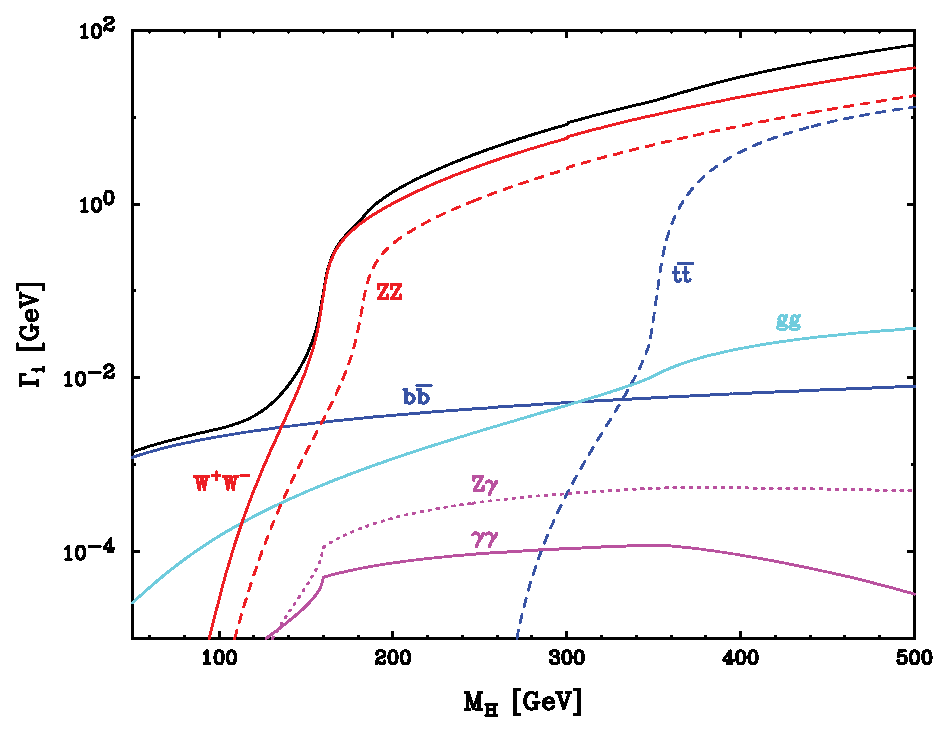
\includegraphics[width=\textwidth]{theory/HiggsDecayWidth}
        \caption{}
        \label{fig:theoryHiggsDecayWidth}
    \end{subfigure}
    \begin{subfigure}[b]{0.45\textwidth}
        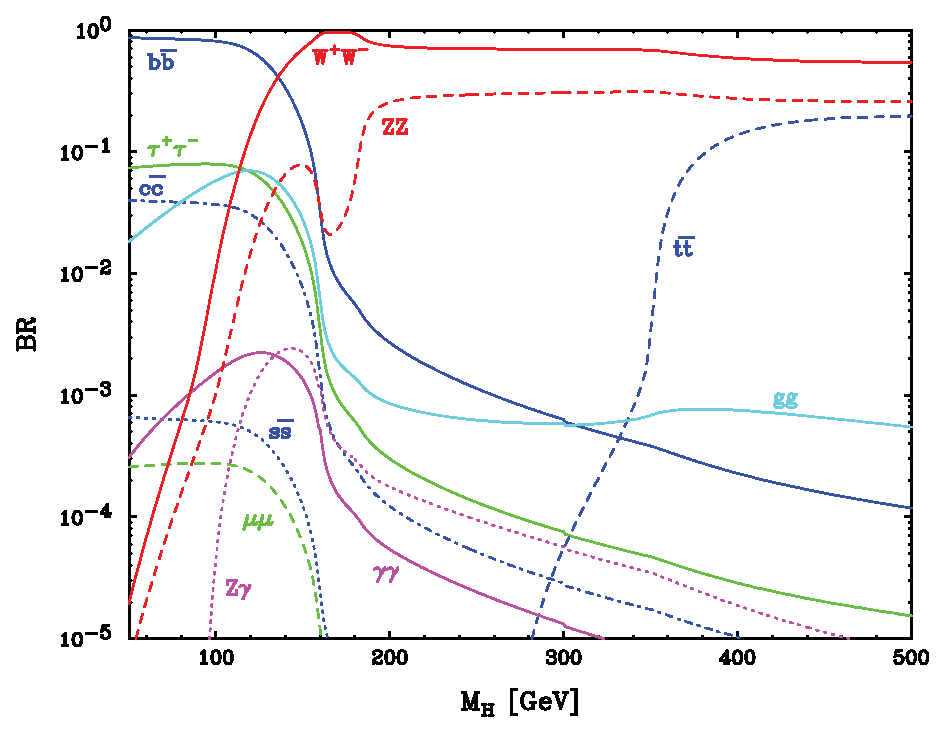
\includegraphics[width=\textwidth]{theory/HiggsBranchingRatio}
        \caption{}
        \label{fig:theoryHiggsBranchingRatio}
    \end{subfigure}
\caption[SM Higgs boson decay width and branching ratios]%
{a) the Higgs boson partial decay widths, and b) selected Higgs boson branching ratios, plotted as a function of the Higgs boson mass, $M_{\PH}$. In a), the black curve shows the total decay width. Both figures are taken from \cite{Rainwater:2007cp}.}
\label{fig:theoryHiggsPhenomenology}
\end{figure}


\section{Yukawa couplings}

The Yukawa sector of the electroweak Lagrangian provides the mass terms for quarks and charged leptons after the spontaneous symmetry breaking of the Higgs field. The   $\Lagr_{Yukawa}$ is given by:
\begin{equation}
\Lagr_{Yukawa} = -\lambda^{u}\overline{q_L}\Phi_{\PH}^{c}u_R  - \lambda^{d}\overline{q_L}\Phi_{\PH}{d}_R - \lambda^{e}\overline{l_L}\Phi_{\PH}e_R + h.c. ,
\end{equation}
where $q_L$ is the left-handed quark doublet field; $u_R$ is the up-type right-handed quark singlet field;  $d_R$ is the down-type right-handed quark singlet field; $l_L$ is the left-handed lepton doublet field; $e_R$ is the right-handed charged lepton singlet field; $\lambda$ is a constant; $\Phi_{\PH}^{c} \equiv i \sigma^2{\PH}^*$ is an SU(2) doublet field with hypercharge $Y = -\frac{1}{2}$; and  the Lagrangian is summed over all possible quarks and leptons. When the Higgs vacuum expectation value is substituted in the $\Lagr_{Yukawa}$, the interaction terms become mass terms:
\begin{equation}
m_{u} = \frac{\lambda^u{\nu}}{\sqrt{2}},\ m_{d} = \frac{\lambda^d{\nu}}{\sqrt{2}},\ m_{e} = \frac{\lambda^e{\nu}}{\sqrt{2}}.
\end{equation}


\section{Higgs beyond the Standard Model}
\label{sec:theoryHiggsBSM}

Because of issues that can not be explained by the \SM, a number of BSM Higgs theories have been proposed. The light Higgs could be a composite bound state of new strongly-interacting sector at the TeV scale. If the composite Higgs is the pseudo Nambu-Goldstone boson from a spontaneous global symmetry breaking, the Higgs can be naturally light \cite{Kaplan:1983fs}.  The couplings of the Higgs would deviate to those in the \SM at a high energy.



An important physics channel for testing the Higgs theory is the double Higgs production via vector boson fusion at high energy \cite{Giudice:2007fh,Contino:2010mh,Contino:2013gna}. For the composite Higgs scenario, the scattering amplitude of this channel increases with energy. It is difficult for the Large Hadron Collider to measure the double Higgs production due to the large \SM background rate \cite{Contino:2010mh}. However, a multi-TeV linear electron-position collider, such as the Compact Linear Collider, would be able to measure the cross section for the this process \cite{Barger:2003rs}.

The study of double Higgs production via \WW fusion can probe the Higgs trilinear self coupling, \gHHH, and quartic coupling, \gWWHH. Leading-order Feynman diagrams for double Higgs production via \WW fusion are shown in \Figure{fig:theorydoubleHiggsFeynman}. The diagram shown in  \Figure{fig:theorydoubleHiggsFeynman1} contains the triple Higgs vertex, which is sensitive to the Higgs trilinear self coupling \gHHH. The diagram in the \Figure{fig:theorydoubleHiggsFeynman2} is sensitive to the quartic coupling \gWWHH. Figures \ref{fig:theorydoubleHiggsFeynman3} and \ref{fig:theorydoubleHiggsFeynman4} show the Feynman diagrams for irreducible background processes for the study of \gHHH and \gWWHH.

\begin{figure}[!htbp]
  \begin{subfigure}[b]{0.22\textwidth}
    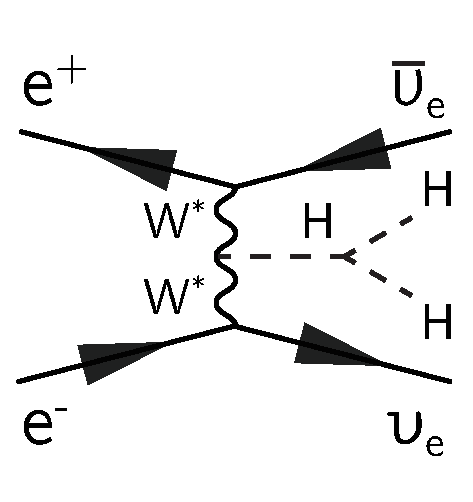
\includegraphics[width=\textwidth]{{{doubleHiggs/Feynman/1}}}
    \caption{}
    \label{fig:theorydoubleHiggsFeynman1}
  \end{subfigure}
  \begin{subfigure}[b]{0.22\textwidth}
    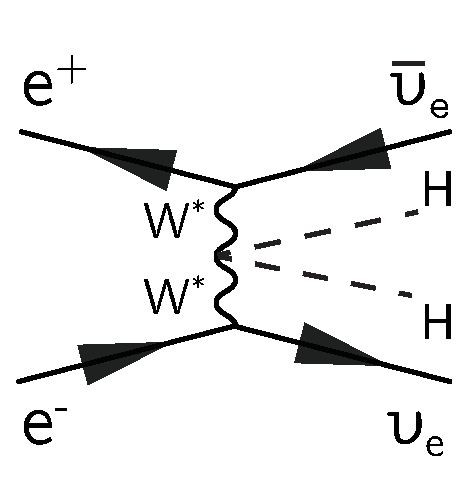
\includegraphics[width=\textwidth]{{{doubleHiggs/Feynman/2}}}
    \caption{}
    \label{fig:theorydoubleHiggsFeynman2}
  \end{subfigure}
  \begin{subfigure}[b]{0.22\textwidth}
    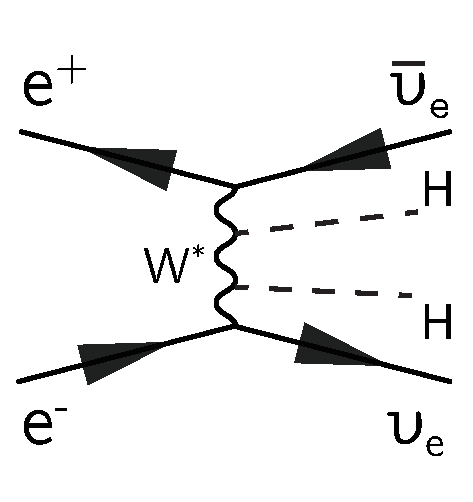
\includegraphics[width=\textwidth]{{{doubleHiggs/Feynman/3}}}
    \caption{}
    \label{fig:theorydoubleHiggsFeynman3}
  \end{subfigure}
  \begin{subfigure}[b]{0.22\textwidth}
    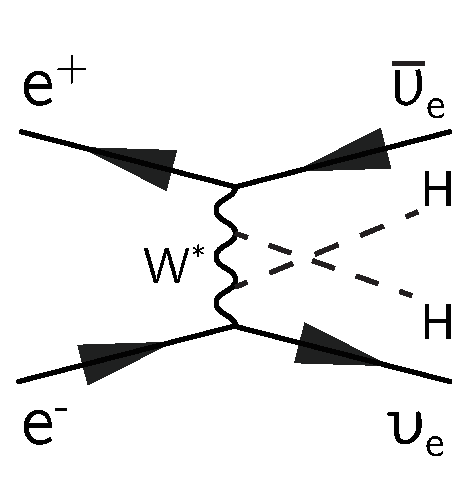
\includegraphics[width=\textwidth]{{{doubleHiggs/Feynman/4}}}
    \caption{}
    \label{fig:theorydoubleHiggsFeynman4}
  \end{subfigure}
\caption
   {The main Feynman diagrams for the leading-order \eeToHH processes.}
   \label{fig:theorydoubleHiggsFeynman}
\end{figure}

Following the assumption made in  \cite{Contino:2010mh,Contino:2013gna}, the self interaction of the light scalar Higgs, $h$, and its coupling to other \SM bosons can be described by a Lagrangian using the notation in  \cite{Contino:2013gna}. After the electroweak symmetry breaking with vacuum expectation value $\nu \approx$246\,GeV, the  Lagrangian is given by:
\begin{equation}
\Lagr =\frac{1}{2}\left(\partial_\mu{h}\right)^2  - V(h) + \parenths{m_W^2{W}_\mu^+{W}^{-\mu} + \frac{m_Z^2}{2}Z_{\mu}Z^\mu}\sqbracs{1 + 2a\frac{h}{\nu} + b \frac{h^2}{\nu^2} + \hdots},
\end{equation}
where $V(h)$ is the $h$ field potential
\begin{equation}
V(h) = \frac{1}{2}m_h^2h^2 + d_3\parenths{\frac{m_h^2}{2\nu}}h^3 + d_4\parenths{\frac{m_h^2}{8{\nu}^2}}h^4 + \hdots ,
\end{equation}
and $a$, $b$, $d_3$ and $d_4$ are  dimensionless parameters; higher order terms in $h$ are omitted; the parameters $a$ and $b$ are proportional to the coupling strength of the $VVh$ and $VVhh$ vertices, where $V$ represents vector boson: \PWpm and \PZ; and the parameters $d_3$ and $d_4$ are proportional to the trilinear and quadlinear $h$ self coupling strength, respectively. Comparing with the  $\Lagr_{Higgs} $ in the \SM,  the \SM implies $a=b=d_3=d_4=1$, and all higher order terms vanish. However, BSM Higgs theories allow $a,b,d_3,d_4$ to take different values.

Consider a pair of the longitudinal polarised  vector boson (${V}_L$) coupling to two $h$ field, the scattering amplitude for \HepProcess{{V}_L{V}_L \to hh} can be written as:
\begin{equation}
A = a^2\parenths{A_{SM} + A_1\delta_b + A_2\delta_{d_3}},
\end{equation}
where $A_{SM}$ is the \SM amplitude and:
\begin{equation}
\delta_b \equiv 1 - \frac{b}{a^2},
\end{equation}
\begin{equation}
\delta_{d_3} \equiv 1 - \frac{d_3}{a}.
\end{equation}
The term $A_1$ grows like the squared of energy at a large center-of-mass energy, $E\gg{m_V}$. The terms $A_{SM}$ and $A_2$ have no energy dependence. Therefore, the parameter $\delta_b$ controls the magnitude of the increasing of the scattering amplitude as a function of energy. The parameter $\delta_{d_3}$, on the other hand, determines the magnitude at the higgs mass threshold. In an electron-positron collider, this scattering process can be studied via the double Higgs production \HepProcess{\Ppositron\Pelectron \to \Pneutrino\APneutrino hh} channel. The cross section can be written as
\begin{equation}
\label{eq:theoryGeneralHiggsCrossSection}
\sigma = a^4\sigma_{SM}\parenths{1 + A\delta_b + B\delta_{d_3} + C\delta_b\delta_{d_3} + D\delta_b^2 + E\delta_{d_3}^2},
\end{equation}
where $\sigma_{SM}$ is the \SM cross section. Suitable observables are variables that increase with the increasing of the centre-of-mass energies. Two examples of such variables are the invariant mass of the two Higgs system, $m_{hh}$, and the scalar sum of two Higgs transverse momenta, $H_T$. \FIGURE{fig:theoryMhhHtDistribution} shows that the $m_{hh}$ and $H_T$ distributions are sensitive to the values of $\delta_{b}$ and $\delta_{d_3}$  \cite{Contino:2013gna}. Around the \SM value of $\delta_{d_3}$, a large value of $\delta_{b} $(0.3) produces events with large values of $m_{hh}$ and $H_T$. By studying the  $m_{hh}$ and $H_T$ distributions, the change in the  $m_{hh}$ and $H_T$ distributions can be related to the  change in $\delta_{b}$ and $\delta_{d_3}$. Therefore a study of sensitivity of the $\delta_{b}$ and $\delta_{d_3}$ can be established using the $m_{hh}$ and $H_T$ distributions. It should be noted that the \Figure{fig:theoryMhhHtDistribution} is obtained from a generator-level study.

\begin{figure}[htbp]
\centering
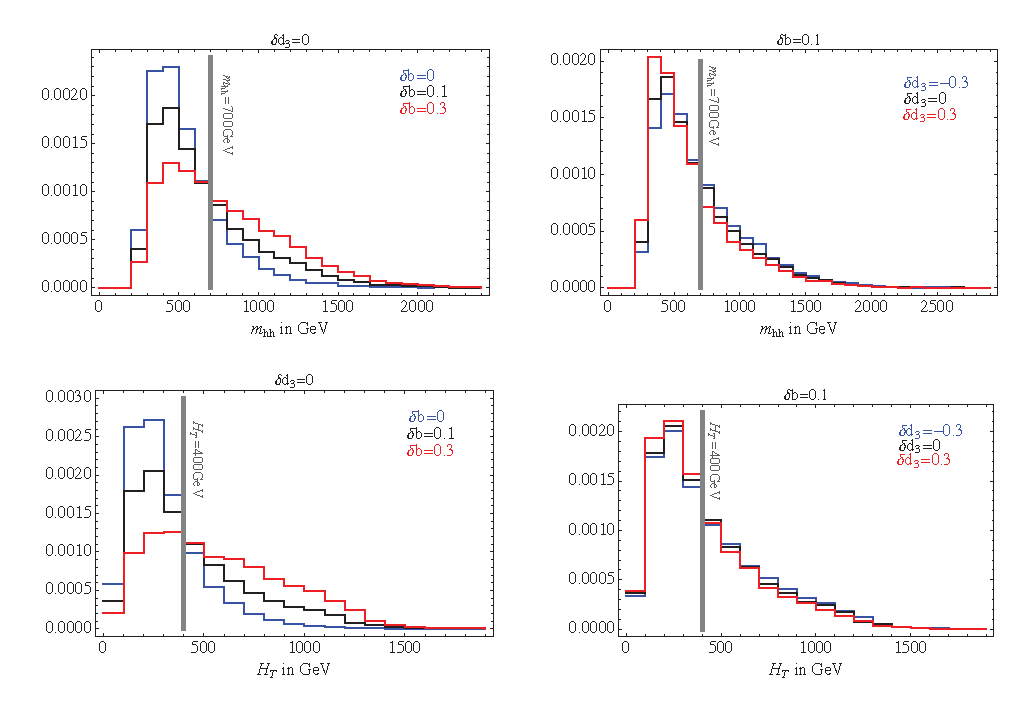
\includegraphics[width=1\textwidth]{theory/MhhHtDistribution}
\caption[]
{Normalized differential cross sections $d\sigma/dm_{hh}$ and $d\sigma/dH_{T}$ for \HepProcess{\Ppositron\Pelectron \to \Pneutrino\APneutrino hh} at the Compact Linear Collider, with \rootS{3} after the identification cuts, for several values of $\delta_{b}$ and $\delta_{d_3}$. The plot is taken from \cite{Contino:2013gna}.}
\label{fig:theoryMhhHtDistribution}
\end{figure}

In the cross section of the double Higgs production via \HepProcess{\Ppositron\Pelectron \to \Pneutrino\APneutrino hh}  in \Equation{eq:theoryGeneralHiggsCrossSection}, the parameter $a$, which is proportional to $g_{VVH}$, enters as an overall factor. At the same time, $a$ also appears in the definition of $\delta_{b}$ and $\delta_{d_3}$. Hence a three-dimensional fit of the parameters $a$, $\delta_{b}$, and $\delta_{d_3}$ would be needed to extract the values of the$a$, $\delta_{b}$, and $\delta_{d_3}$. However,  for a multi-TeV electron-positron collider, the cross section for single Higgs production is far greater than that of the double Higgs production. Consequently, the measurement of the parameter $a$, using  \HepProcess{\Ppositron\Pelectron \to \Pneutrino\APneutrino h}  channel, would be performed before the measurement of the $\delta_{b}$ and $\delta_{d_3}$ for the double Higgs production.  \FIGURE{fig:theoryHiggsCrossSection} shows the comparison of cross sections as a function of the centre-of-mass energy, for different the Higgs production modes. Up to a centre-of-mass energy of \rootS{3}, the cross sections of the single Higgs production are two orders of magnitude larger than the cross sections of the double higgs production. Therefore, for the purpose of measuring $g_{VVHH}$ and $g_{HHH}$ via double Higgs production, it is sufficient to treat the parameter $a$ as a known constant. Hence only a two-dimensional fit of the parameters $\delta_{b}$, and $\delta_{d_3}$ would be performed.

\begin{figure}[!htbp]
\centering
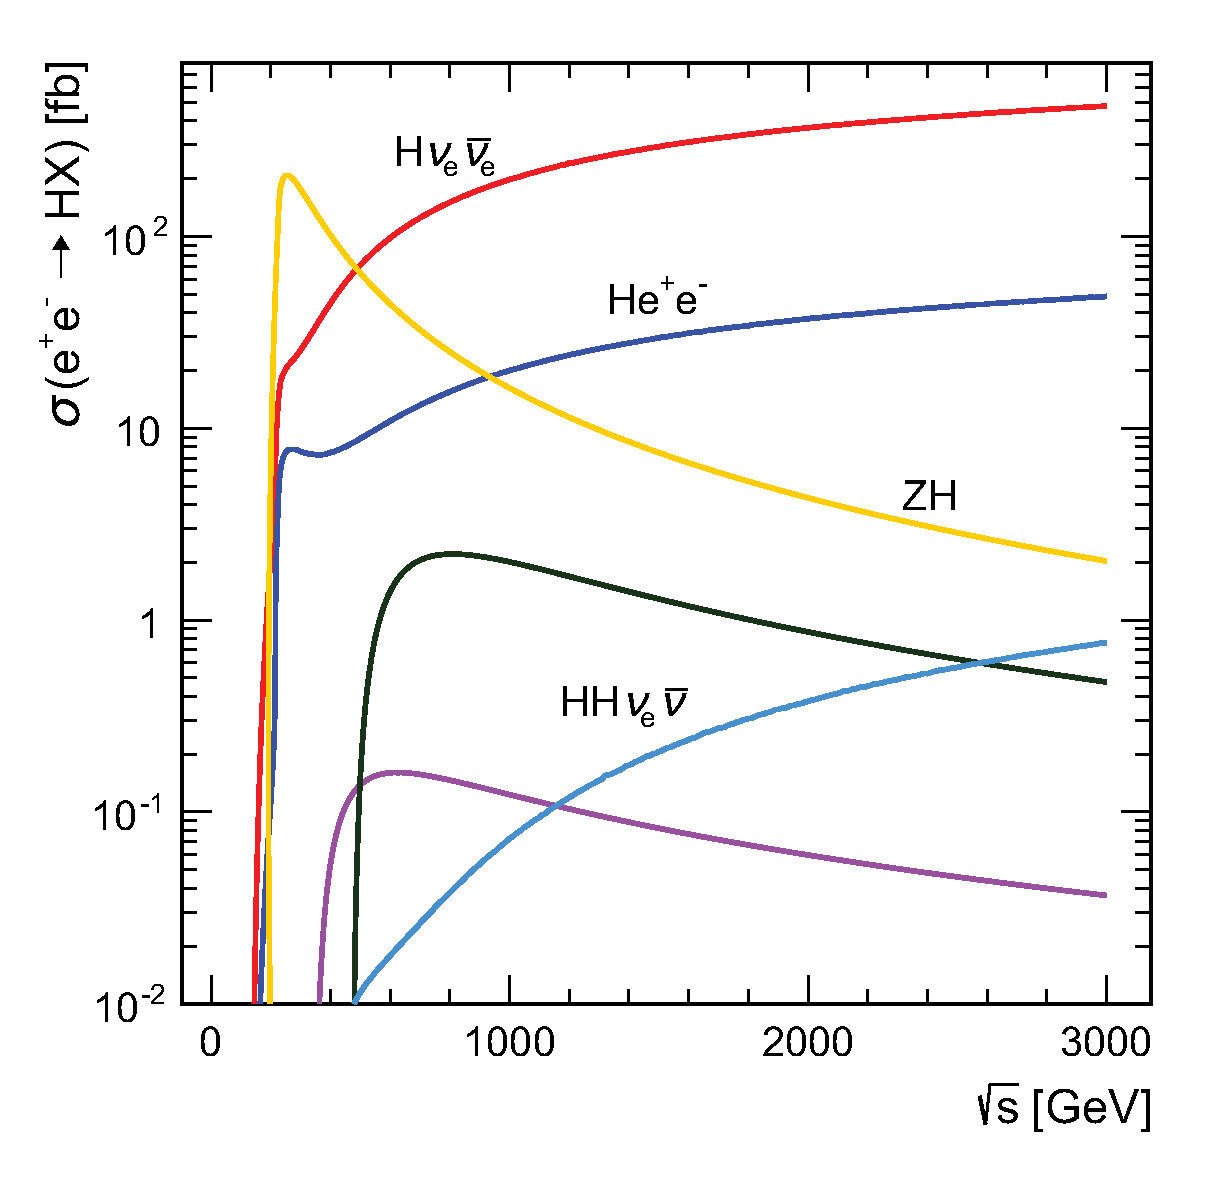
\includegraphics[width=0.45\textwidth]{theory/HiggsCLICcrossSection}
\caption[]
{Cross section as a function of centre-of-mass energy for the Higgs production processes at an electron-positron collider for a Higgs mass of 126\,GeV. The values shown correspond to unpolarised beams and do not include the effect of beamstrahlung. The plot is taken from \cite{Abramowicz:2016zbo}.}
\label{fig:theoryHiggsCrossSection}
\end{figure}


\section{Tau pair polarisation correlations as a signature of Higgs boson}
\label{sec:theoryTauPair}


The tau lepton is an fundamental particle similar to the electron, with negative electric charge and a spin of $\frac{1}{2}$. It has the same interaction properties as an electron, but a much larger mass. The tau lepton has a corresponding anti-particle of opposite charge but equal mass and spin. Tau mean lifetime is $(290.3\pm0.5)\times10^{-15}$\,s. Tau has many decay modes. Decay modes with branching ratio above 2\% are listed in table \Table{tab:theoryTauDecayMode}.

% The most difficult final states to separate are \decayRhoFinalStateShort and \decayAiPhotonFinalStateShort, where photons from boosted \Ppizero are very challenging to reconstruct correctly.

\begin{table}[htbp]\centering
\smallskip
\begin{tabular}{l l r}
\hline
\hline
Decay mode &  Branching ratio\\
\hline
\decayElectron     & $17.83\%_{\pm0.04\%}$   \\
\decayMuon  & $17.41\%_{\pm0.04\%}$  \\
\decayPion  	& $10.83\%_{\pm0.06\%}$   \\
\decayRho   & $25.52\%_{\pm0.09\%}$ \\
\decayAi   	& $9.30\%_{\pm0.11\%}$    \\
\decayAi      & $8.99\%_{\pm0.06\%}$  \\
\decayThreePionPhoton      & $2.70\%_{\pm0.08\%}$  \\
\hline
\hline
\end{tabular}
\caption[Decay modes, detectable final state particles and branching ratios of the seven major \Pgtm decays.]
{Decay modes, detectable final state particles and branching ratios of the seven major \Pgtm decays, taken from \cite{Agashe:2014kda}. \Pgtp decays similarly to \Pgtm.}
\label{tab:theoryTauDecayMode}
\end{table}

A scalar Higgs boson with spin-0 would decay to \TauTauSub{L}{L} or \TauTauSub{R}{R}; A vector boson \PZ with spin-1, on the other hand,  decays to \TauTauSub{L}{R} or \TauTauSub{R}{L}, where L, R denotes the tau lepton helicities. Therefore, by studying the tau pair polarisation correlation from a boson decay, one could identify if the parent boson is a  scalar Higgs boson or a vector \PZ boson.

%For many theories beyond the Standard Model, a common feature is that the coupling of the Higgs particle to leptons increases with the increase of the lepton mass \cite{Duperrin:2008in}.  In these BSM theories, unlike vector bosons coupling to all flavours of leptons equally, the \HigssTauTau coupling would dominate the Higgs coupling to leptons. Therefore, if an experiment observes the breaking of the lepton universality by favouring \TauTau events, it could indicate the existence of a scalar Higgs. When such a universality breaking is observed, a helicity correlation test can be used to show that the \TauTau pair is from a scalar boson or a vector boson. In particular, the polarisation correlations of tau leptons are different for \HiggsToTauTau and \ZToTauTau, as scalar Higgs decays to \TauTauSub{L}{L} or \TauTauSub{R}{R} and \PZ decays to \TauTauSub{L}{R} or \TauTauSub{R}{L}, where L, R denotes the tau lepton helicities.


Tau pair polarisation correlations can be studied using various tay decay modes. Here \Reference{Bullock:1991my} is followed and the \tauToPion decay mode is used as the example. The Higgs and \PZ boson decay to tau pair  via  \tauToPion can be represented as:
\begin{equation}
\HepProcess{X \to \TauTauSub{\alpha}{\beta} \to \Ppiplus\Ppiminus  + \Pneutrino{s}},
\end{equation}
where $X$ is either \PHiggs or \PZ; and $\alpha$, $\beta$ are the helicities, L or R. In the collinear limit where $m^2_{\Ptau}/m^2_X \ \ll \ 1$, the appropriate kinematic variables are the energy fractions:
\begin{equation}
\overline{z} = \frac{E_{\Ppiplus}}{E_{\APtauon}},\text{and}\ z = \frac{E_{\Ppiminus}}{E_{\Ptauon}}.
\end{equation}
For a single tau decay, the differential cross section distribution can be written as:
\begin{equation}
\frac{1}{\Gamma_{\Ptau}}\frac{d\Gamma}{dz} = Br_{\parenths{\tauToPion}} f\parenths{\HepProcess{\TauFull{\alpha}{-} \to \Ppiminus} ; z},
\end{equation}
where $Br_{\parenths{\tauToPion}}$ is the branching fraction of \tauToPion. The form $f$ can be obtained by working outing the matrix element from the Feynman diagram and integrating  the squared of the matrix element over the phase space \cite{Tsai:1971vv}:
\begin{equation}
f\parenths{\HepProcess{\TauFull{\alpha}{-} \to \Ppiminus} ; z} = 1 + P_\alpha\parenths{2z-1},
\end{equation}
where $P_L = -1$ and $P_R = +1$. Hence for the tau pair decay, the differential cross section distribution is of the form:
\begin{equation}
\frac{d^2N\parenths{\HepProcess{X \to \TauTau \to \Ppiplus\Ppiminus  + \Pneutrino's}}}{dz\,d\overline{z}} = Br^2_{\parenths{\tauToPion}} \sum_{\alpha,\,\beta}^{} C^X_{\alpha \beta} f\parenths{\HepProcess{\TauFull{\alpha}{-} \to \Ppiminus} ; z} f\parenths{\HepProcess{\TauFull{\beta}{+} \to \Ppiplus} ; \overline{z}},
\end{equation}
where the only non-zero correlation coefficients $C_{\alpha \beta}$ for the parity-conserving \HiggsToTauTau are:
\begin{equation}
C^{\PHiggs}_{LL} = C^{\PHiggs}_{RR} = \frac{1}{2},
\end{equation}
and the non-zero correlation coefficients  for the  \ZToTauTau are:
\begin{equation}
C^{\PZ}_{LR} = \frac{1}{2}\parenths{1 - P_{\Ptau}},\ C^{\PZ}_{RL} = \frac{1}{2}\parenths{1 + P_{\Ptau}},
\end{equation}
where non-zero tau polarisation, $P_{\Ptau}$, is because  \ZToTauTau  is not parity-conserving in the \SM:
\begin{equation}
P_{\Ptau} = \frac{-2va}{v^2 + a^2},
\end{equation}
where the parameter $v= -\frac{1}{2} + \sin^2{\theta_{\PW}},$ and  the parameter $a= -\frac{1}{2}$ are the vector and axial-vector \ZTauTau couplings, respectively.


\FIGURE{fig:theoryTauPairCorrelation} shows two-dimensional distributions of  $\frac{E_{\Ppiplus}}{E_{\APtauon}}$ as a function of $\frac{E_{\Ppiminus}}{E_{\Ptauon}}$ using both \tauToPion channel for \ZToTauTau and \HiggsToTauTau. The difference of the tau pair polarisation correlation between \PZ and \PHiggs  is clear. The energy distribution of the pion from \ZToTauTau has the form of $f\sim z$, whilst from  \HiggsToTauTau has the form of $f\sim (1-z)$. Therefore, in \ZToTauTau, a high-energy \Pgppm (a large $z$) is likely to be associated with a high-energy \Pgpmp (a large $\overline{z} $); in \HiggsToTauTau, the opposite is favoured. If the tau pair decay from Higgs boson is observed, the decay can be recognised in the \tauToPion mode as a high-energy \Pgppm with a low-energy \Pgpmp. Hence, the tau decay product energy distribution can be a clean signature for \HiggsToTauTau.

%Photon - passage through matter. Photon electromagnetic shower

\begin{figure}[htbp]
\centering % \begin{center}/\end{center} takes some additional vertical space
%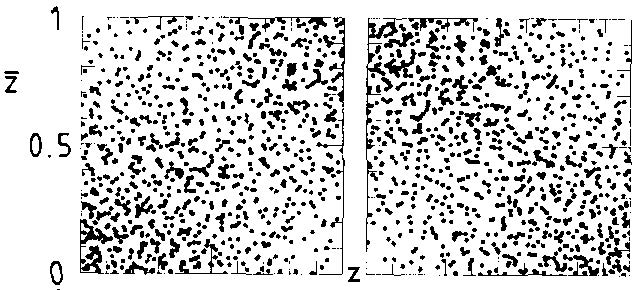
\includegraphics[width=0.9\textwidth]{theory/TauPairCorrelation.jpg}
  \begin{subfigure}[t]{0.45\textwidth}
    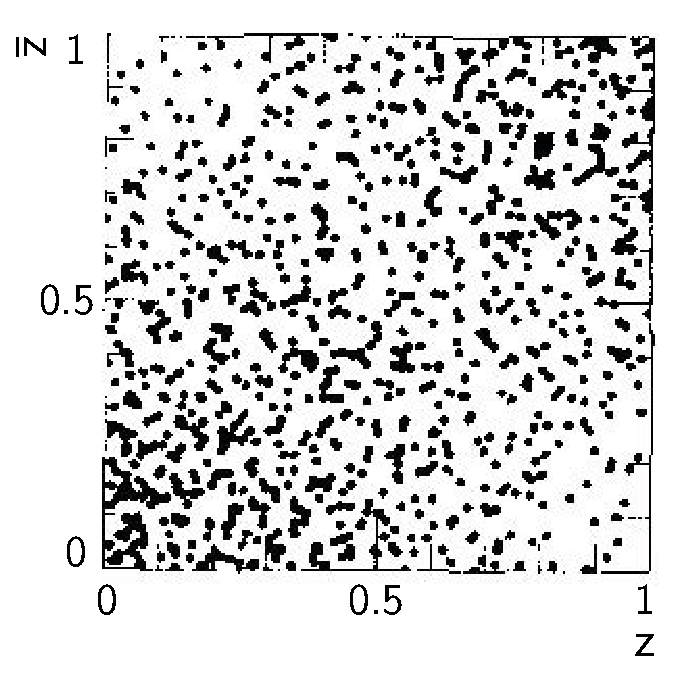
\includegraphics[width=\textwidth]{theory/TauZ}
    \caption{\ZToTauTau}
    \label{fig:theoryTauPairCorrelationZ}
  \end{subfigure}
  \begin{subfigure}[t]{0.45\textwidth}
    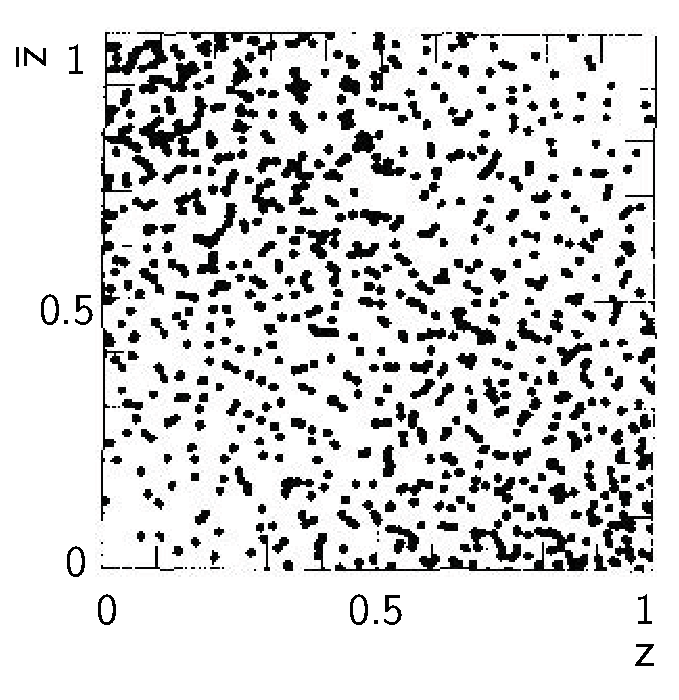
\includegraphics[width=\textwidth]{theory/TauH}
    \caption{\HiggsToTauTau}
    \label{fig:theoryTauPairCorrelationH}
  \end{subfigure}
\caption[Two-dimensional distribution of \ZToTauTau and \HiggsToTauTau.]
{Two-dimensional distribution of $\overline{z} ={E_{\Ppiplus}}/{E_{\APtauon}}$ as a function of $ z ={E_{\Ppiminus}}/{E_{\Ptauon}}$  using both \tauToPion channel for a) \ZToTauTau, and b) \HiggsToTauTau.  Both figures are adapted from reference \cite{Tsai:1971vv}.}
\label{fig:theoryTauPairCorrelation}
\end{figure} 
  \chapter{Detectors}
\label{chap:Detector}

\chapterquote{The great man is the one who does not lose his child's heart.}%
{Mencius, 372 BC - 289 BC}%: Blackwood's Magazine May 1830


Since the discovery of a particle consistent with the Standard Model Higgs boson at the LHC in 2012 \cite{Aad:2012tfa,Chatrchyan:2012ufa}, the natural step for high energy physicists is to understand the Higgs. Yet limited by the underlying QCD interaction from proton-anti-proton collision, one has great difficulties in measuring the properties of the Higgs precisely. However, next generation electron-positron linear colliders could make precise measurements in the Higgs sector, as well as the top quark sector \cite{Brau:2007zza,Linssen:2012hp}.

\section{The \ILC}

Two leading candidates for next generation electron-positron linear colliders are the International Linear Collider (\ILC) \cite{Brau:2007zza}, and the Compact Linear Collider (\CLIC) \cite{Linssen:2012hp}. The \ILC is a high-luminosity electron-positron linear collider with centre-of-mass energies from 200\,GeV up to 1\,TeV. The machine would be built at different stages. The first stage would have a centre-of-mass energy of 250/350\,GeV. The second stage would have a centre-of-mass energy of  500\,GeV with a possible upgrade to 1\TeV. Thirty years of development leads to the technical design report in 2013 \cite{Baer:2013cma}. A layout of the collider complex is shown in \Figure{fig:detectorILC}. The proposal contains two detector concepts, the International Large Detector (\ILD) and the Silicon Detector (\SiD).

\begin{figure}[tbph]
\centering
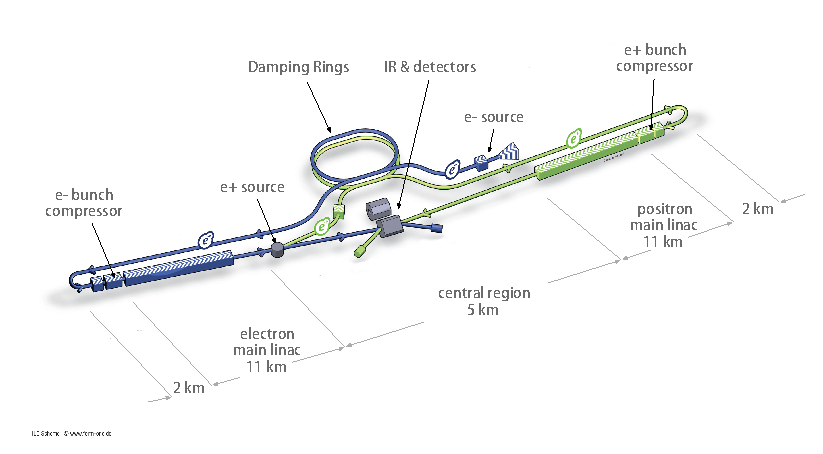
\includegraphics[width=0.85\textwidth]{ILD/ILC2}
\caption
{A layout of the International Linear Collider complex, taken from \cite{Baer:2013cma}.}
\label{fig:detectorILC}
\end{figure}


\begin{comment}
The International Linear Collider (ILC) is a high-luminosity linear electron-positron collider based on
1.3 GHz superconducting radio-frequency (SCRF) accelerating technology. Its centre-of-mass-energy
range is 200�C500 GeV (extendable to 1TeV). A schematic view of the accelerator complex, indicating
the location of the major sub-systems, is shown in Fig. 3.1:

The International Linear Collider (ILC) is a 200�C500 GeV (extendable to 1TeV) centre-of-mass highluminosity
linear electron-positron collider, based on 1.3 GHz superconducting radio-frequency (SCRF)
accelerating technology. Its parameters have been set by physics requirements first outlined in 2003,
updated in 2006, and thoroughly discussed over many years with the physics user community. The
physics parameters have been reviewed continuously and found to be robust to advances in the science,
including the recent discovery of a Higgs boson at the Large Hadron Collider at CERN.

The collider design is the result of nearly twenty years of R&D. The heart of the ILC, the
superconducting cavities, is based on over a decade of pioneering work by the TESLA collaboration in
the 1990s. Some other aspects were based on the R&D carried out for the JLC/GLC and NLC projects,
which were based on room-temperature accelerating structures. Since 2005, the design of the ILC
accelerator has continued as a worldwide international collaboration coordinated by the Global Design
Effort (GDE) under a mandate from the International Committee for Future Accelerators (ICFA).
Drawing on the resources of over 300 national laboratories, universities and institutes worldwide, the
GDE produced the ILC Reference Design Report (RDR) in August 2007. The work done by the GDE
during the RDR phase identified several high-risk challenges that required R&D, which have since
been the focus of the worldwide activity during the Technical Design Phase. In parallel with the
accelerator effort, detailed baseline designs of two detectors have been developed by large international
teams as a result of intense detector R&D under the coordination of the Research Directorate, also
established by a mandate of ICFA.
\end{comment}

\section{The \CLIC}

The other potential next-generation electron-positron linear collider,  the Compact Linear Collider (\CLIC) \cite{Linssen:2012hp}, has a higher reach of the centre-of-mass energy, up to 3\,TeV. The \CLIC is designed to built in stages as well.  The first stage, with a centre-of-mass energy of 380\,GeV, is a compromise of precision measurement between top quark physics and Higgs physics. The final stage of a centre-of-mass energy of 3\,TeV is motivated by the physics reach of detecting new physics  and measuring rare decays of Higgs. The second stage has a centre-of-mass energy of 1.4\,TeV, which bridges between the first stage and the final stage. A layout of the \CLIC complex is shown in \Figure{fig:detectorCILC}. Due to the similarities of the two linear collider programs, the development with the \CLIC detector concepts started with the \ILC detector concepts. Two  \CLIC detector concepts, the \CLICILD and the \CLICSiD, are developed based on the \ILD and the \SiD, respectively.

%Although the accelerating systems would be different, the calorimeter designs are similar, both highly granular for the optimal particle flow.


\begin{figure}[tbph]
\centering
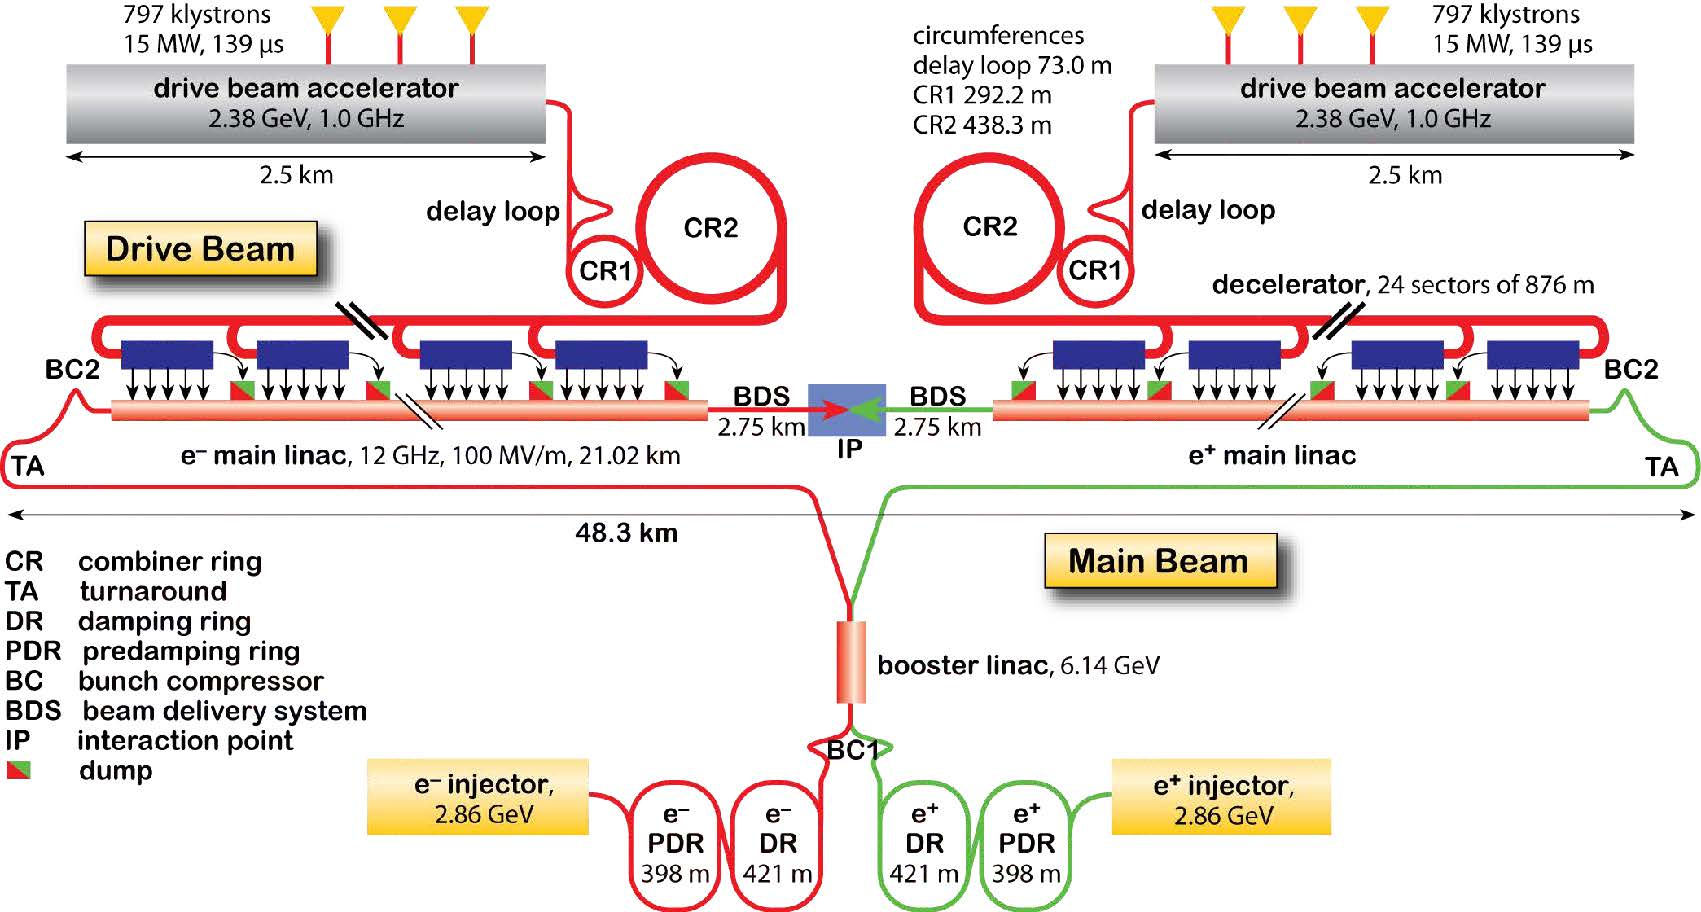
\includegraphics[width=0.85\textwidth]{ILD/CLIC}
\caption
{A layout of the Compact Linear Collider at final stage of a centre-of-mass of energy of  3\,TeV, taken from \cite{Aicheler:2012bya}.}
\label{fig:detectorCILC}
\end{figure}

\begin{comment}
The ILC has developed two detector models, namely the International Large Detector (ILD) \cite{Abe:2010aa} and the Silicon Detector (SiD) \cite{Aihara:2010zz}. The CLIC has developed two slightly modified detector models based on ILD and SiD \cite{Linssen:2012hp}. One key common feature of these next generation electron-positron linear colliders is the high granular calorimeter, which provides a great spatial resolution at the cost of the energy resolution. Particle flow algorithms (PFA) benefit from the spatial resolution from calorimeters, together with tracking information, to provide excellent a jet energy resolution. PandoraPFA, the most complicated and the best performing one, provides a jet energy resolution of less than 3.5\%, which is required for W/Z separation \cite{Thomson:2009rp,Marshall:2013bda}.
\end{comment}





\section{Physics at future linear colliders}

The physics program for the \CLIC and the \ILC, which is a driving force for the detector design, share some common goals. \ILC has a reach of a centre-of-mass energy from 200\,GeV to 1\,TeV, whilst \CLIC can reach a centre-of-mass energy from 350\,GeV to 3\,TeV. Both machines are capable of precision higgs coupling measurements, top mass and coupling measurements, and search for new physics such as supersymmertry particles. The \ILC can also operate at low energy to be a \PZ and a \PHiggs factory for ultra precise \PZ mass and \PHiggs mass measurements. \CLIC, on the other hand, has the advantage of a higher energy reach, which allows measurements of rare events, such as higgs trilinear self-couplings and quartic couplings.


\section{Impact of physics requirements on the detector design}

\subsection{Jet energy resolution requirements on the detector design}
\label{sec:detectorPhysicsRequirementPandora}

The physics goal of jet energy resolution at the \ILC and the \CLIC is to separate \PW and \PZ, using \Wqq and \Zqq channels, by reconstructing the invariant mass via quark-jets \cite{Baer:2013cma,Linssen:2012hp}. This translates to a requirement of 3.5-5\% of the jet energy resolution. This level of precision is unlikely to be achieved with a traditional calorimetry design. A traditional energy flow approach to calorimetry measures jet energies as a sum of the energy in the calorimeters. The jet energy resolution is parameterised by:
\begin{equation}
\frac{\sigma_{E}}{E} = \frac{\alpha}{\sqrt{E(GeV)}}\oplus\beta .
\end{equation}
The stochastic term $a$ is typically greater than 60\% and $b$ is of the order of a few percents. For the jet energy resolution of 3.5\%, $a$  should be less than 30\%, which is unlikely to be achieved by a traditional calorimeter.  On the contrary, the particle flow approach to calorimetry  has demonstrated it ability to reach the goal \cite{Thomson:2009rp,Marshall:2012ry}.

In a typical jet, using measurements of the particle composition from the \LEP\cite{Knowles:1997dk,green1998electron}, about 62\% of the jet energy is from charged particles, 27\% from photons, 10\% from long-lived neutral hadrons, and 1.5\% from neutrinos. In a traditional approach to calorimetry, about 72\% jet energy is measured in the electromagnetic (\ECAL) and the hadronic (\HCAL) calorimeters combined. The jet energy resolution is thus limited by the energy resolution of the hadronic calorimeters, which typically is $\gtrsim 55\% / \sqrt{E(GeV)}$ \cite{Behnke:2013lya}.

The particle flow approach to calorimetry improves the jet energy resolution by fully reconstructing  all visible particles in the detector. The jet energy is the sum of energy of individual particles, where the energy of the charge particles are measured in the tracking detectors, and the energy of neutral particles are measured in calorimeters. In this approach, the hadronic calorimeter only measures about 10\% of the energy, which would greatly improve the overall energy measurement. Assuming 30\% of the jet energy (photon energy) is measured with ${\sigma_{E}}/{E} = 15\% / \sqrt{E(GeV)}$, and 10\% of the jet energy (hadron energy) is measured with ${\sigma_{E}}/{E} = 55\% / \sqrt{E(GeV)}$ \cite{Behnke:2013lya}, a jet energy of ${\sigma_{E}}/{E} = 19\% / \sqrt{E(GeV)}$ can be obtained. This satisfies the jet energy resolution requirement for separating \PW and \PZ via their hadronic decays. In reality, this level of performance is unattainable due to incorrect association of energy deposits to particles. At jet energies beyond tens of GeVs, the ``confusion'' rather than the intrinsic detector performance limits the particle flow performance.

The particle flow calorimetry requires to fully reconstruct particles and to associate calorimeter hits to tracks in tracking detectors. This is a demanding task for the software design and the detector design. The software details of the \pandora, which is a successful particle flow implementation, are described in \Section{sec:pandoraPandoraPFA}. For the detector design, the detector needs to be highly granular for an excellent spatial resolution, which is needed to correctly associate calorimeter hits to the inner detector tracks. This imposes stringent requirements in the \ECAL and the \HCAL designs.


 %and it is illustrated with a brief description of the particle flow principle.

\begin{figure}[tbph]
\centering
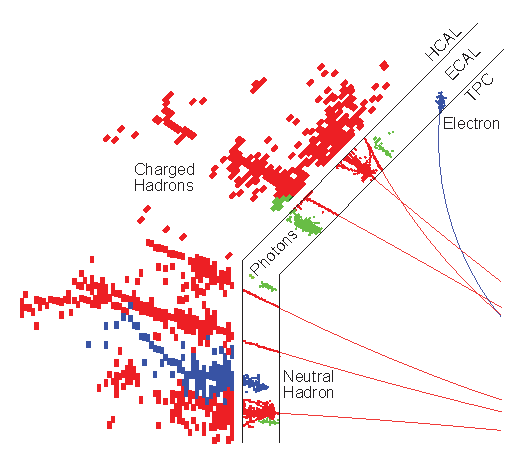
\includegraphics[width=0.45\textwidth]{{ILD/jetCLIC_ILD}}
\caption[A typical topology of a 250\,GeV jet.]
{A typical topology of a 250\,GeV jet, simulated with thr \CLICILD detector concept, taken from \cite{Marshall:2012ry}.}
\label{fig:detectorJetCLICILD}
\end{figure}


\FIGURE{fig:detectorJetCLICILD} shows a typical topology of a 250\,GeV jet, simulated with the \CLICILD detector concept. Particles consisting of the calorimeter hits and tracks are labelled with different colours. Clusters of calorimeter hits in the highly granular \ECAL and \HCAL are associated with tracks from the inner tracking detector, time projection chamber (\TPC). Photons are identified using the characteristics longitudinal and transverse electromagnetic shower profiles. Hadronic showers are separated from electromagnetic showers due to the small transverse spread of the electromagnetic shower.  The inner tracking detector should be highly efficient and have very little material. For the calorimeter, the \ECAL and \HCAL, both should be highly granular. The material of the calorimeter should be dense and has a large ratio of interaction length to radiation length.

\subsection{Other requirements on the detector design}

Other physics requirements for the detectors for the \ILC and the \CLIC are summarised in \cite{Baer:2013cma,Linssen:2012hp}. Here important requirements are presented as motivations for detector designs.


The performance requirement of the vertex detector is determined by the required performance of b-quark and c-quark tagging. The ability to identify secondary vertices and tracks, which are not originated from the interaction point, is the prerequisite for the flavour tagging. The impact parameter resolution can be written in the form of:
\begin{equation}
\sigma_{d_0}^2 = a^2 + \frac{b^2}{p^2\sin^2\left(\theta\right)},
\end{equation}
where $a$ is related to the point resolution and $b$ is related to multiple scattering. The requirements for both the \ILC and the \CLIC detectors are $a \lesssim 5 \mu{m}$ and $b \lesssim 15 \mu{m}\,GeV$ \cite{Behnke:2013lya,Linssen:2012hp}.


The requirement of tracking momentum resolution is driven by the Higgs boson mass resolution via the Higgsstrahlung process, \eeTo{\PZ \PHiggs}. The Higgs mass can be reconstructed precisely as the recoil mass against the \PZ momenta, which is obtained via \HepProcess{\PZ \to \APmuon \Pmuon}. For the \ILC operating at \rootSGeV{250}, the momentum resolution needs to be  $\sigma_{\pT} / \pT^2 \lesssim 5 \cdot 10^{-5}$\,\uprightMarth{GeV^{-1}} \cite{Behnke:2013lya}. For the \CLIC at a higher  centre-of-mass energy, the momentum resolution needs to be  $\sigma_{\pT} / \pT^2 \lesssim 2 \cdot 10^{-5}$\,\uprightMath{GeV^{-1}} \cite{Linssen:2012hp}.

The lepton identification should be over 95\% for effective lepton tagging. The forward converge of the detector should be down to a very low angle, i.e. a few mrad, with respect to the beam axis. This is more critical for the \CLIC as particles are boosted at a high centre-of-mass energy.

\section{The International Large Detector}

Two detector concepts have been designed for the \ILC to deliver the physics program. The motivation for two detectors is to have multiple independent measurements within one collider for cross-checking, complementary measurements, and competition between collaborations. The two detectors are both designed to be general purpose detectors. The Silicon Detector, \SiD, is a compact detector with a large magnetic filed of 5\,T. It uses silicon tracking modules. The second detector, the International Large Detector, \ILD, is a larger detector with a time projection chamber as the main tracking unit. Both detectors have highly granular calorimeters optimised for the particle flow. A view of both detector concepts can be seen in \Figure{fig:detectorILDSiD}

%Precision tests for the Standard Model requires an excellent jet energy resolution and mass reconstruction. Particle low algorithms (PFA), based event reconstruction, meet the requirements. For the best performance of the PFA, high granular calorimeter systems and highly efficient tracking systems are needed. The requirement to separate \PW and \PZ bosons in hadronic decay final states requires a jet energy resolution below 3.5\%. The momentum resolution of $5\times10^{-5}$\,GeV is motivated by the Higgs boson recoil reconstruction in the Higgsstrahlung.




The International Large Detector, the \ILD, is a detector concept at the \ILC. The \ILD detector concept has been optimised in the view of the particle flow techniques. Particle flow approach to event reconstruction has shown to deliver the best possible jet reconstruction with proof-of-principle implementation such as \pandora. Each individual particle is reconstructed with the particle flow algorithms. For charged particles, calorimeter hits are associated with the tracks. Therefore measurements of charged particles rely on an excellent momentum resolution from the tracking system. Neutral particles reconstruction requires a high spatial resolution of the calorimeters.

The particle flow paradigm requires topological information of individual particle reconstructions. The sub-detector systems need to have the spatial resolution to separate charged particles from neutral particles. The result is a highly granular calorimeter and a central tracking system with excellent momentum resolution. Longitudinal cross section of top quadrant of the \ILD detector concept is shown in \Figure{fig:ILD}. From the interaction point (\IP) outwards, there is a tracking system comprising a large time projection chamber (\TPC) augmented with silicon tungsten layers, highly granular electromagnetic calorimeters (\ECAL) and hadronic calorimeters (\HCAL), muon chambers, forward calorimeters (\FCAL), magnetic coils and iron yokes.

The section below will describe the sub-systems of the \ILD detector concept referred to as the ILD\_o1\_v05 option in \Mokka simulation in the \ILD technical design report\cite{Baer:2013cma}. This detector concept has been optimised \cite{Abe:2010aa} and used in studies described in subsequent chapters.

The \CLICILD detector concept for the \CLIC in the conceptual design report\cite{Linssen:2012hp} is a modified version of the \ILD, adapted to the \CLIC colliding environment. As they share similarities, an overview of the \ILD sub-detectors is provided, followed by a discussion on the difference between the \ILD and the \CLICILD detector concepts.  A comparison of the longitudinal cross section of the top quadrants of between \ILD and \CLICILD can be seen in \Figure{fig:detectorILD}. A comparison of the key parameters between the \ILD and the \CLICILD can be found in \Table{tab:ILDvsCLICILD}.





\begin{figure}[tbph]
\centering
  \begin{subfigure}[t]{0.45\textwidth}
    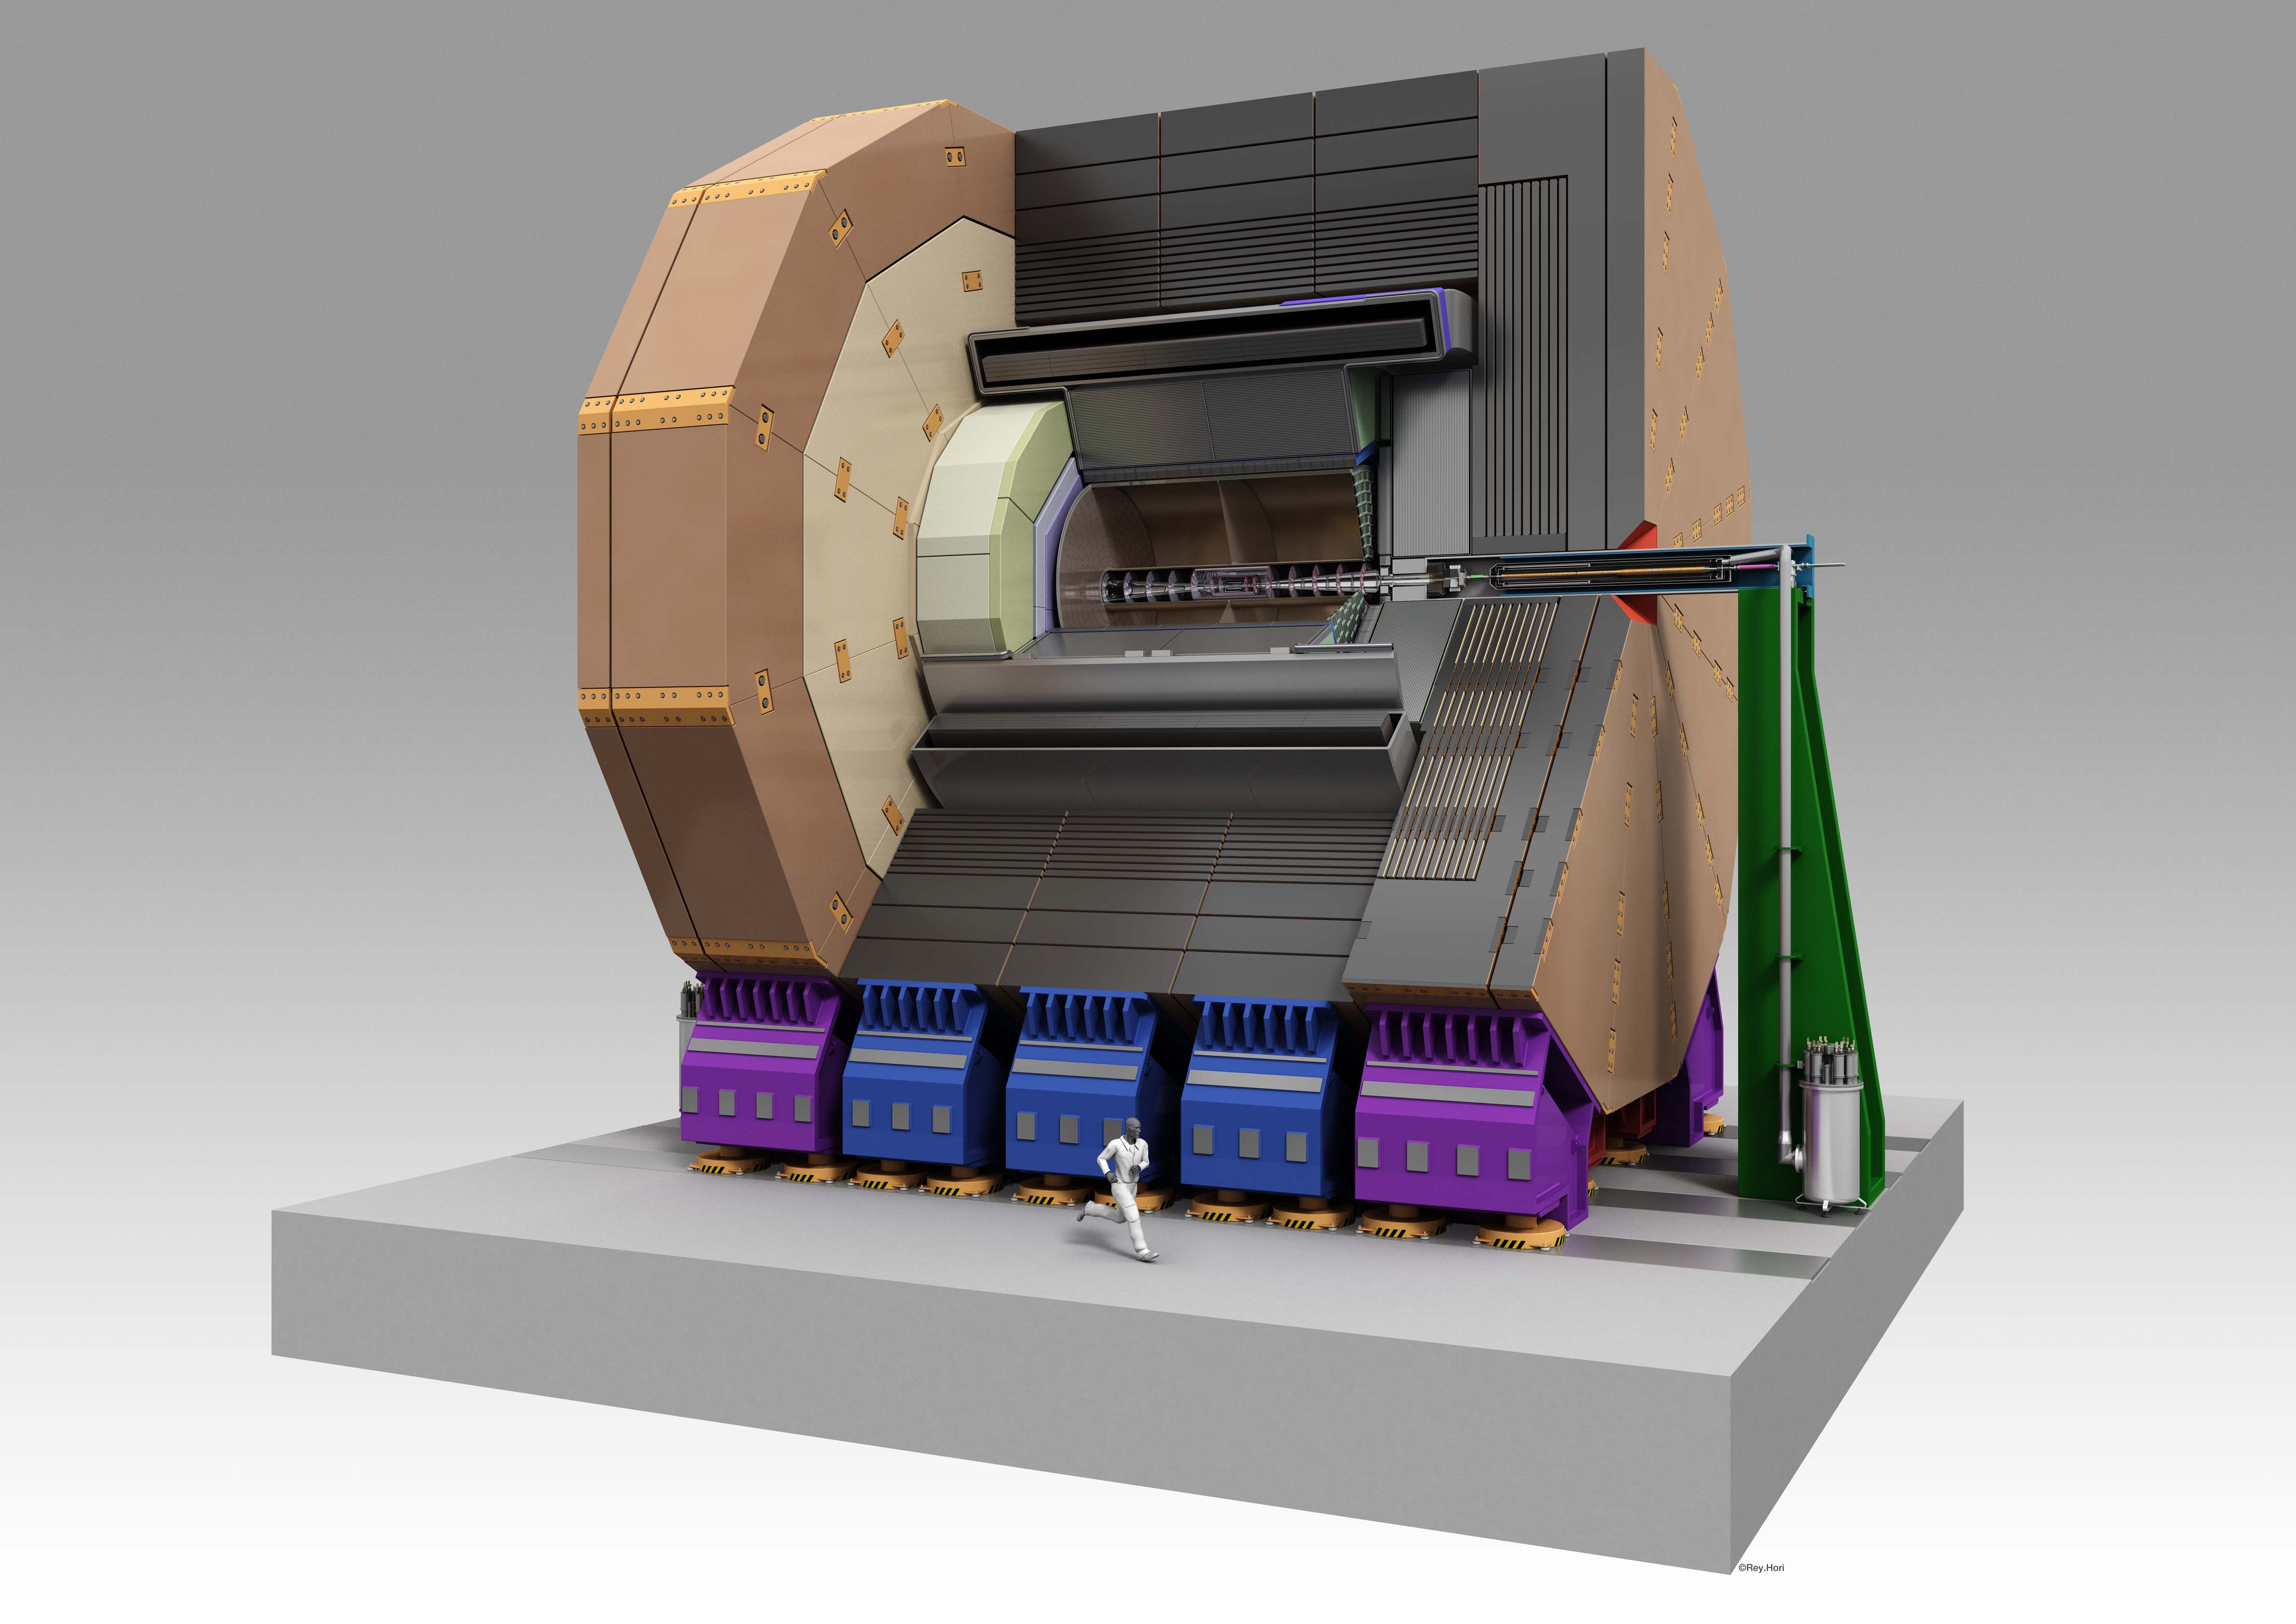
\includegraphics[width=\textwidth]{ILD/ILDview}
    \caption{}
    \label{fig:ILDview}
  \end{subfigure}
  \begin{subfigure}[t]{0.46\textwidth}
    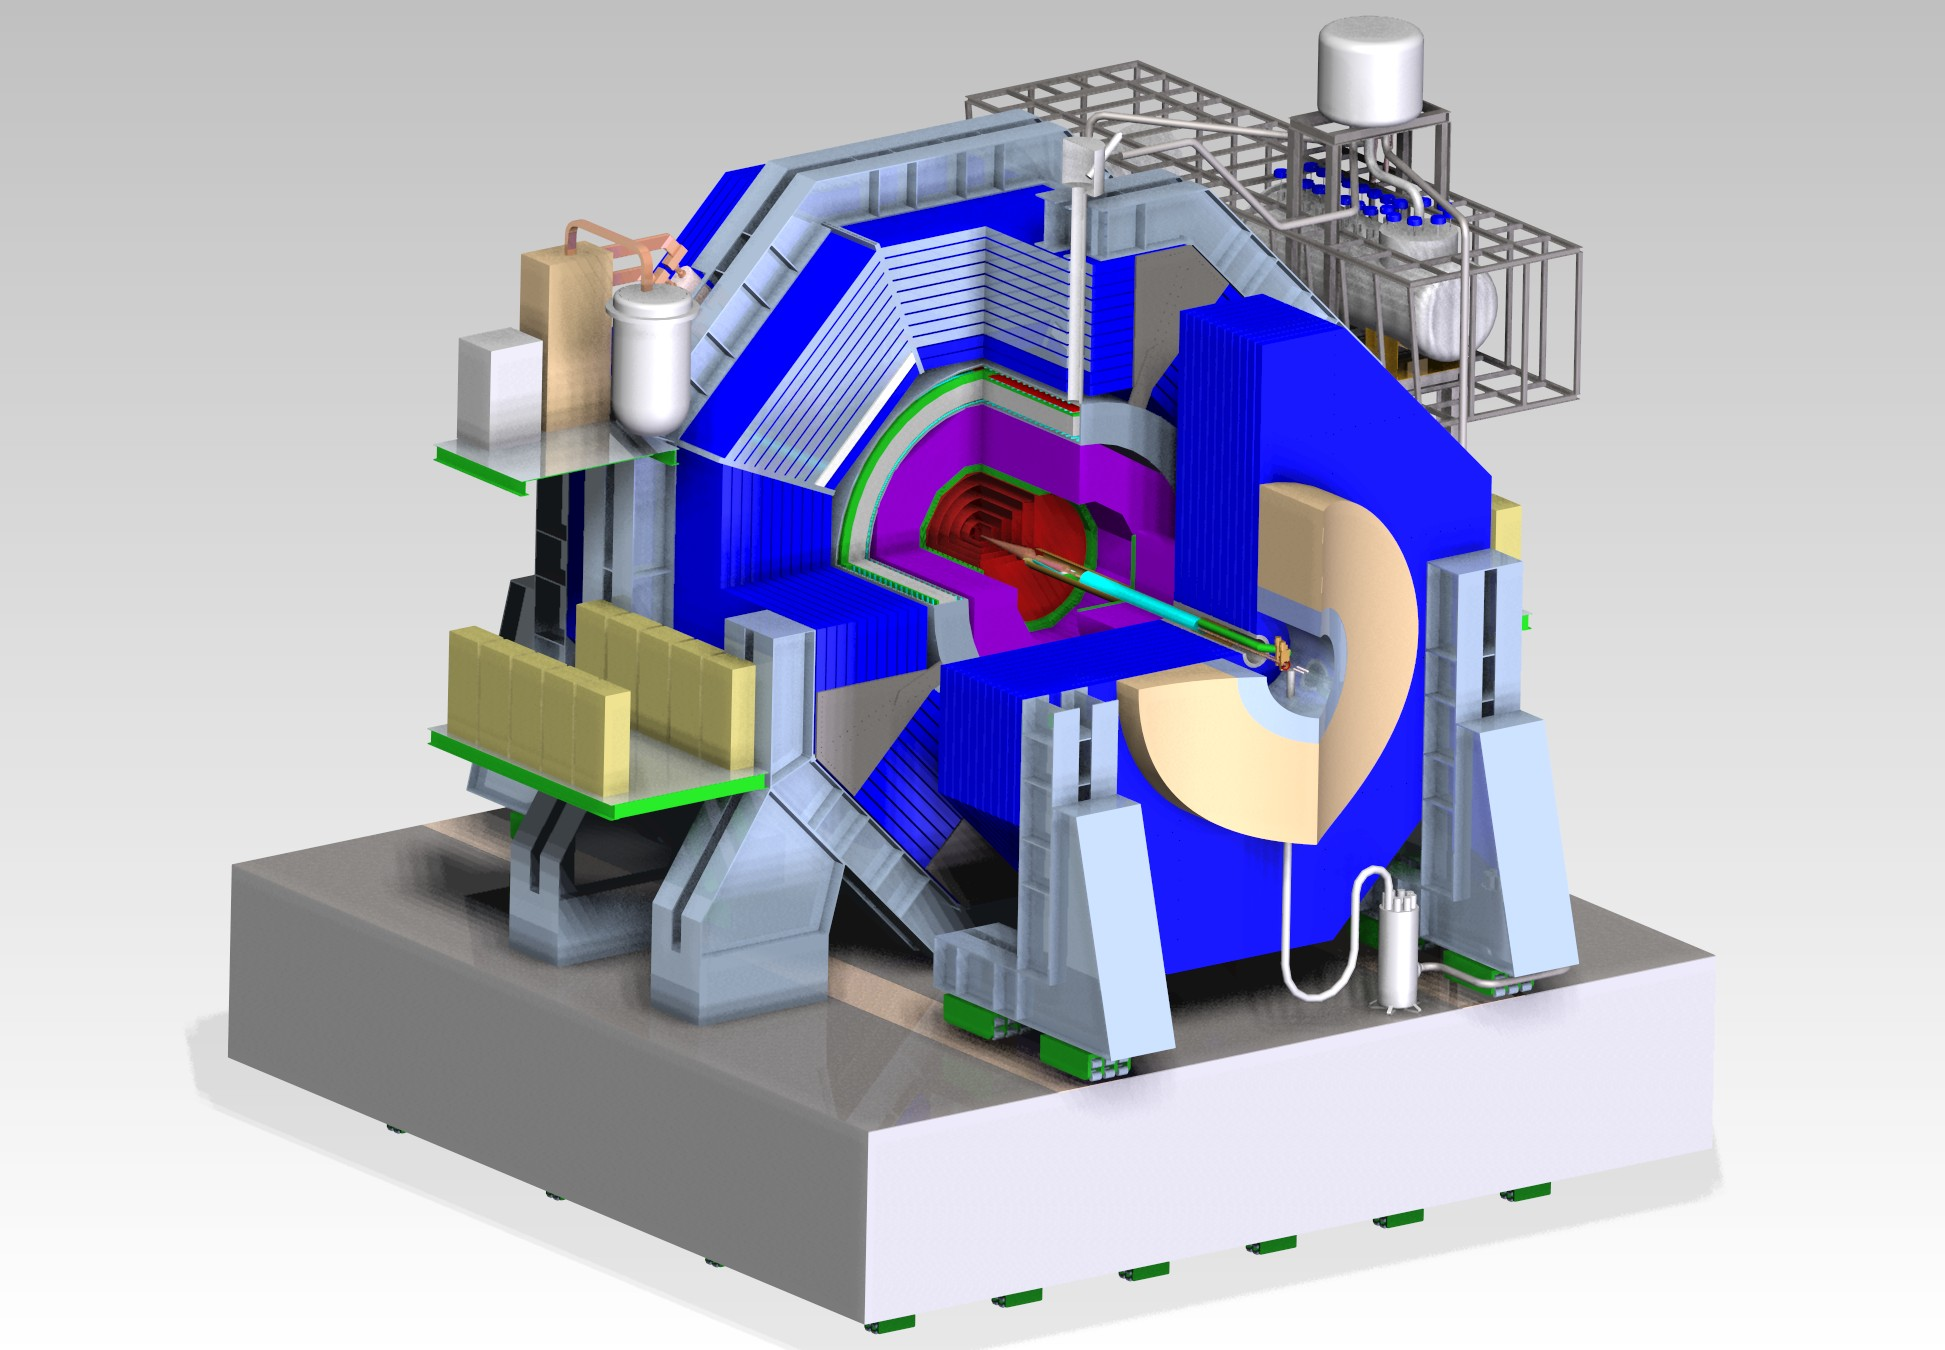
\includegraphics[width=\textwidth]{ILD/SiD}
    \caption{}
    \label{fig:SiDview}
  \end{subfigure}
\caption[International Large Detector and the Silicon Detector for the International Linear Collider.]
{a) the International Large Detector, and b) the Silicon Detector. Both detector concepts are designed for the International Linear Collider. Both figures are  taken from \cite{Baer:2013cma}.}
\label{fig:detectorILDSiD}
\end{figure}

\begin{comment}
The ILC has been designed to enable two experiments (SiD and ILD) sharing one interaction region using
a push-pull approach. This two-detector design is motivated by the enhanced scientific productivity of
past collider facilities which benefited from independent operation of multiple experiments, providing
complementary strengths, cross-checking and confirmation of results, reliability, insurance against
mishaps, competition between collaborations, as well as increased number of involved scientific
personnel. Figure 4.1 shows the arrangement of the two detectors in the detector hall.
Both detector designs are conceived as multi-purpose detectors, optimised for the broad range
of physics opportunities at the ILC. SiD is a compact, cost-constrained detector made possible
with a 5 Tesla magnetic field and silicon tracking. Silicon enables time-stamping on single bunch
crossings to provide robust performance, derived from immunity to spurious background bursts. The
highly granular calorimeter is optimised for particle-flow analysis. The ILD group has designed a
large detector with robust and stable performance over a wide range of energies. The concept uses
a tracking system based on a continuous-readout time-projection chamber combined with silicon

In order to realise the physics program, the ILC detectors face challenges requiring significant advances
in collider detector performance. The machine environment is benign by LHC standards, enabling
designs and technologies that are unthinkable at the LHC. However, the ILC environment poses its
own set of background issues that must be overcome. The ��Detailed Baseline Design�� of the SiD and
ILD detectors have been developed to achieve the requirements for all considered physics programs,
over the full range of centre-of-mass energies from 200 GeV up to 1TeV, as well as the possibility of
special running at the Z-pole.
The ILC physics opportunities place a premium on high-resolution jet energy reconstruction and
di-jet mass performance. Event reconstruction techniques based on the Particle Flow Algorithm (PFA)
have been developed to meet this challenge. This motivates highly granular electromagnetic and hadron
calorimeters and highly efficient tracking systems. New detector technologies and new reconstruction
algorithms based on the PFA approach achieve the needed precision in the reconstruction of jets of 3
to 4 percent for 100 GeV jets, set by the requirement to separate W and Z di-jet final states. The
requirements on momentum resolution for charged tracks (p/p2 of 5 �� 10.5 (GeV/c).1) are driven
by reconstruction of a Higgs boson recoiling from the associated Z boson decaying to a lepton pair in
the Higgs-strahlung process. Flavour and quark-charge tagging will be available at an unprecedented
level of performance as a result of the development of a new generation of vertex detectors. Particle
identification is achieved by the highly granular calorimeters and muon identification is aided by the
instrumented iron return yoke.
A very important element of the detector design work has been the common effort to develop and
apply simulation tools to realise realistic detector-performance estimates. A small group of experts
from both SiD and ILD have cooperated closely on this critical work.
To preserve this unprecedented performance, the inner detectors must accommodate very lowmass
detectors and supports. This is a significant challenge. The detector designs have achieved the
required light-weight support structures with minimal dead spaces. This was greatly simplified by the
ILC time structure of 1 millisecond bunch trains at 5 Hertz. This very sparse filling allows power for
many of the detector subsystems to be switched off between bunch trains (so-called power pulsing),
reducing the heat load and the need for cooling. The design of these power-pulsed systems presents a
significant challenge, including the need for quiescent currents.
27
\end{comment}


\section{Overview of \ILD sub-detectors}

The \ILD detector concept is designed as a general purpose detector. As shown in \Figure{fig:ILD}, closest to the interaction points are a precision vertex detector and a tracking system. The tracking system consists of silicon tracking components and a time projection chamber. Surrounding the tracking system is a highly granular calorimeter system. The outer solenoid provides a magnetic field of 3.5\,T. The most outer iron return yoke also acts as a muon calorimeter.


\subsection{Vertex Detector}

The pixel-vertex detector (\VTX) needs to be close to the interaction point to reconstruct secondary vertices. As the \TPC is the main tracking  detector, the \VTX mainly measures the impact parameter of tracks. Its structure is  of three double layers with a barrel geometry. The double layers lower the material budget and improves the impact parameter measurements. The first double layer is of the half length of the other two, to avoid the high occupancy region of direct low momentum hits from the incoherent pair background. The baseline geometry of the vertex detector can be found in \Table{tab:detectorVertex}.

\begin{table}[htbp]
\centering
\smallskip
\begin{tabular}{l  r r r r r }
\hline
\hline
 &  R & \absOf{z} & $\absOf{\cos\parenths{\theta}}$ & $\sigma$ & Readout time \\
\hline
Layer 1 & 16\,mm & 62.5\,mm & 0.97 & 2.8\,$\mu$m & 50 \,$\mu$s \\
Layer 2 & 18\,mm & 62.5\,mm & 0.96 & 6\,$\mu$m & 10 \,$\mu$s \\
\hline
Layer 3 & 37\,mm & 125\,mm & 0.96 & 4\,$\mu$m & 100 \,$\mu$s \\
Layer 4 & 39\,mm & 125\,mm & 0.95 & 4\,$\mu$m & 100 \,$\mu$s \\
\hline
Layer 5 & 58\,mm & 125\,mm & 0.91 & 4\,$\mu$m & 100 \,$\mu$s \\
Layer 6 & 60\,mm & 125\,mm & 0.90 & 4\,$\mu$m & 100 \,$\mu$s \\
\hline
\hline
\end{tabular}

\caption
{ Vertex detector parameters. The spatial resolution ($\sigma$) and readout times are for the CMOS option. The table is adapted from \cite{Behnke:2013lya}.}
\label{tab:detectorVertex}
\end{table}




\FIGURE{fig:detectorVertexResolution} shows the impact parameter resolution as a function of the particle momentum for  two different particle production angles. The desired impact parameter resolution (dashed line) is achievable.



\begin{figure}[tbph]
\centering
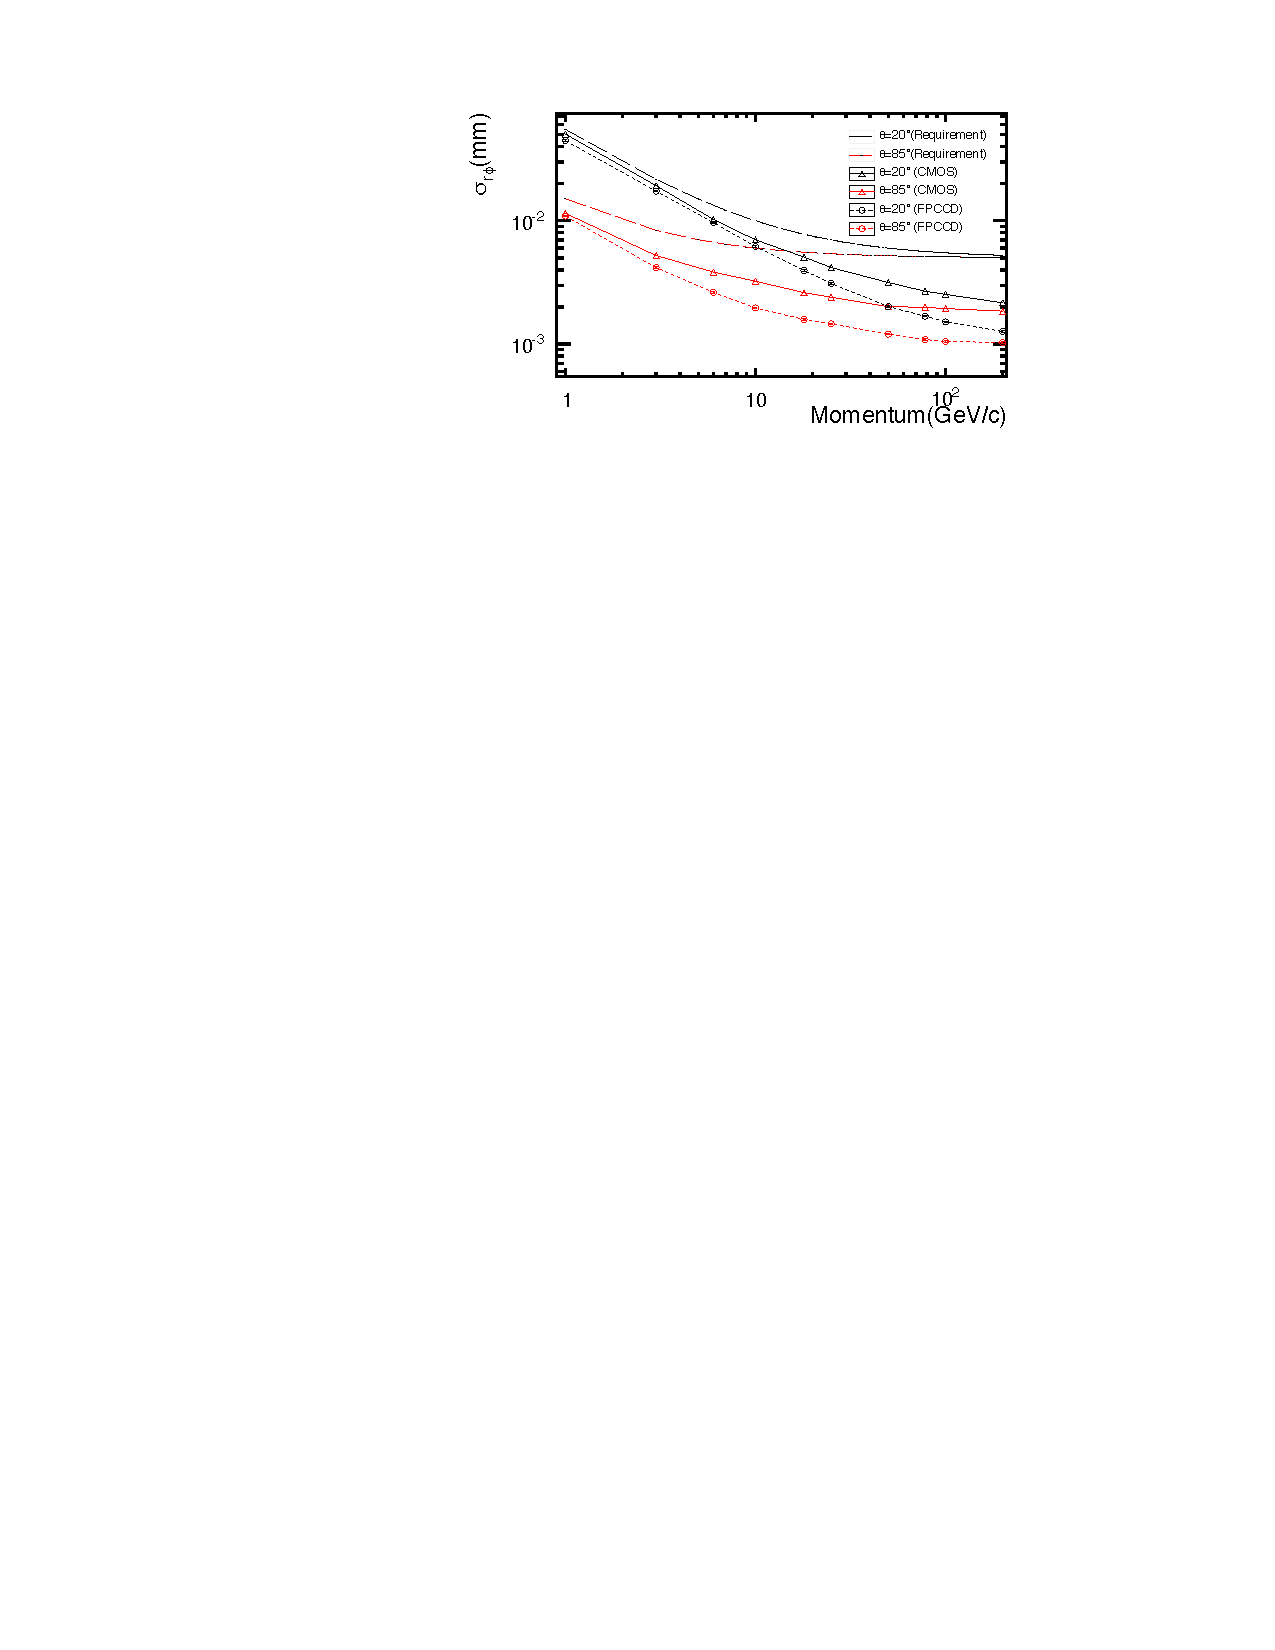
\includegraphics[width=0.55\textwidth]{ILD/vertexResolution}
\caption
{Impact parameter resolution of the \ILD vertex detector for two different particle production angles (20\degree and 85\degree), assuming the baseline point resolution given in \Table{tab:detectorVertex} for CMOS option (solid line), and the FPCCD option (dotted line). The curves with long dashes show the performance goal. The figure is taken from \cite{Behnke:2013lya}.}
\label{fig:detectorVertexResolution}
\end{figure}


\subsection{Tracking Detectors}

The hybrid  tracking system consists of a large time projection chamber (\TPC), a Silicon Inner Tracker (\SIT), a Silicon External Tracker (\SET) in the barrel region, a end cap tracking component (\ETD) behind the endplate of the \TPC, and a silicon forward tracker (\FTD) in the forward region. The \SIT, \SET, and \ETD are made up of two single-sided strip layers tilted by a small angle. The \FTD is a system of two silicon-pixel disks and five silicon-strip disks.  The silicon envelope tracking system and the \TPC are shown in \Figure{fig:detectorTrackingFull}. The main parameters of the silicon system and the \TPC can be found in \Table{tab:detectorTracking}.


The main part of the tracking system, the \TPC, can measure a large number of three dimensional spatial points. Continuous tracking allows precise reconstruction of non-pointing tracks. The \TPC is optimised for point resolution and minimum material, as required for the best calorimeter performance and the best particle flow performance.

The additional barrel silicon trackers improve the overall momentum resolution. They provide extra high precision space points and additional redundancy between the \TPC, the \VTX, and the calorimeters. The \FTD provides the low angle coverage of the tracking system, which is not covered by the \TPC.


\begin{comment}
A system of silicon strip and pixel detectors surrounds the VTX detector. In the barrel, two
layers of silicon strip detectors (SIT) are arranged to bridge the gap between the VTX and the TPC.
In the forward region, a system of two silicon-pixel disks and five silicon-strip disks (FTD) provides
low angle tracking coverage.

The barrel silicon parts SIT and SET provide precise space points before and after the TPC; this
improves the overall momentum resolution, helps in linking the VTX detector with the TPC, and
in extrapolating from the TPC to the calorimeter. The coverage of the TPC with silicon tracking
is completed by the ETD, located within the gap separating the TPC and the end-cap calorimeter.
Together these systems help in calibrating the overall tracking system, in particular the TPC. The
good timing resolution of the silicon detectors relative to the time between bunches in the ILC together
with the high spatial precision helps in time-stamping tracks and assigning them to a given bunch
within an ILC bunch train.
\end{comment}


\begin{table}[htbp]
\centering
\smallskip
\begin{tabular}{l  r r r }
\hline
\hline
 &  R & z & ${\cos\parenths{\theta}}$ \\
\hline
SIT & 153\,mm & 368\,mm & 0.910 \\
SIT & 300\,mm & 644\,mm & 0.902 \\
SET & 1811\,mm & 2350\,mm & 0.789 \\
ETD & 419-1822.7\,mm & 2420\,mm & 0.985-0.799 \\
\hline
TPC  & 329-1808\,mm & $\pm$2350\,mm & up to 0.98 \\
\hline
\hline
\end{tabular}

\caption
{Main parameters of the central silicon systems (SIT, SET, and ETD) and the TPC. The table is adapted from \cite{Behnke:2013lya}.}
\label{tab:detectorTracking}
\end{table}




\begin{figure}[tbph]
\centering
  \begin{subfigure}[b]{0.45\textwidth}
    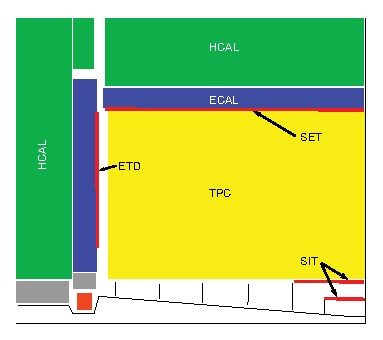
\includegraphics[width=\textwidth]{ILD/Tracking}
    \caption{}
    \label{fig:detectorTracking}
  \end{subfigure}
    \begin{subfigure}[b]{0.45\textwidth}
    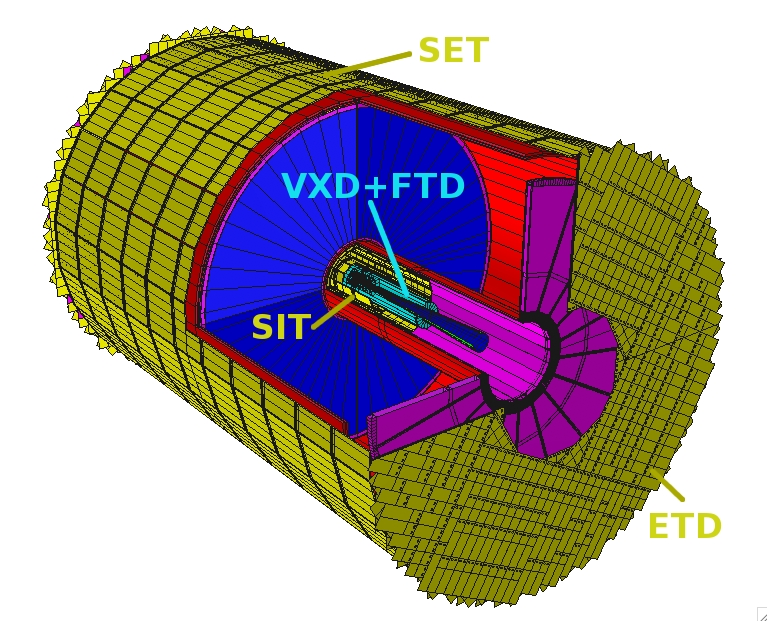
\includegraphics[width=\textwidth]{ILD/ILDtracking}
    \caption{}
    \label{fig:detectorTracking3D}
  \end{subfigure}
\caption
{Plots for a) a top quadrant view of the \ILD silicon envelope system, \SIT, \SET, \FTD, and \ETD, with \TPC, \ECAL, and \HCAL, and b)  a 3D detailed GEANT 4 simulation description of the
silicon system as sketched in the quadrant view in a). Both plots are adapted from figures in \cite{Behnke:2013lya}.}
\label{fig:detectorTrackingFull}
\end{figure}


\subsection{Electromagnetic Calorimeter}

The Silicon-Tungsten sampling electromagnetic calorimeters in the \ILD consist of a nearly cylindrical barrel and two end cap systems, optimised for particle flow. The fine granular \ECAL is located inside the \HCAL. The \ECAL measures photon energies and separates photons from other particles. The \ECAL also hosts the first part of the hadronic showers and greatly assists the separation of hadronic showers.

The particle flow paradigm has a large impact on the \ECAL design with many requirements. In addition, for the \ECAL to measure and separate photons, it also needs to reconstruct detailed shower profiles to separate electromagnetic showers from hadronic showers, as approximately 50\% of hadronic showers starts in the \ECAL. These requirements can be fulfilled with an excellent three-dimensional granular \ECAL.

From test beam data and simulation studies \cite{Ramilli:2012dva,Adloff:2009zz,Adloff:2013jqa}, a sampling calorimeter with longitudinal and transverse segmentation below one Moli\`{e}re radius and below one radiation length at the front the calorimeter is needed. The most compact design is realised with tungsten as absorber material and silicon pad diodes as active material. A cross section of the \ECAL is shown in \Figure{fig:detectorILDECAL}. Tungsten is a dense material with a large ratio of interaction length to radiation length. This helps to separate electromagnetic showers from hadronic showers by making electromagnetic showers transversely narrow. The choice of thin silicon layers offers a great spatial resolution at a cost of the energy resolution in favour of the particle flow. These silicon pads of 5.1 by 5.1\,mm cover large areas, which are simple and reliable to operate.

The longitudinal segregation is a compromise between the cost and the performance. The total of 30 layers, which is about 20\,cm, provides about 24 radiation lengths. The first 20 layers use 2.1\,mm thick absorber plates, which is twice finer sampling than the last 10 layers with 4.2\,mm   thick absorber plates. The test beam data with electrons shows the energy resolution of the \ECAL concept to be $16.6/\sqrt{E(\ GeV)}\oplus1.1\%$ \cite{Behnke:2013lya}, which is compatible with the values assumed for the full \ILD detector simulation.

The optimisation of the \ECAL design as a function of the number of longitudinal layers is performed, whilst keeping other geometry constant, using the jet energy resolution. The jet energy resolution is defined as the root mean squared divided by the mean for the smallest width of distribution that contains 90\% of entries, using \Zuds sample at barrel region. The angular cut is to avoid the barrel/endcap overlap region. The light quark decay of the \Zprime is used as \pandora does not attempt to recover missing momentum from semi-leptonic decay of heavy quarks. Using 90\% of the entries is robust and focus on the Gaussian part of the distribution. The total jet energy is sampled at 91, 200, 360 and 500\,GeV. \FIGURE{fig:detectorILDECALjer} shows the jet energy resolution for a single jet. For a 45\,GeV jet, a degradation  of 10\% in the jet energy resolution is observed when the number of layers decreases from 30 to 20. The degradation in the jet energy resolution is significant for number of layers fewer than 20, although the impact is smaller for high energy jets.


\begin{figure}[tbph]
\centering
  \begin{subfigure}[b]{0.45\textwidth}
    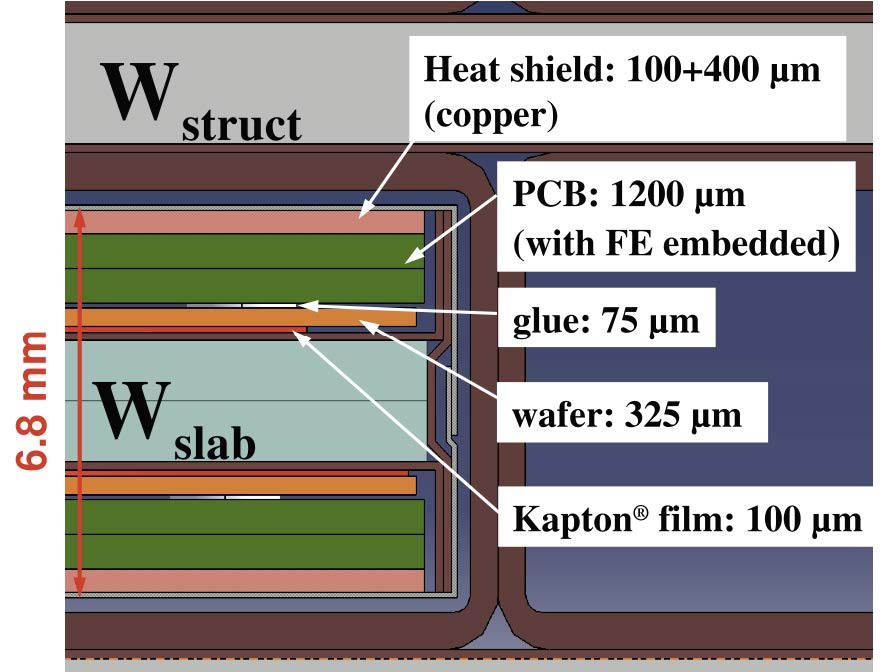
\includegraphics[width=\textwidth]{ILD/ILD_ECAL}
    \caption{}
    \label{fig:detectorILDECAL}
  \end{subfigure}
  \begin{subfigure}[b]{0.45\textwidth}
    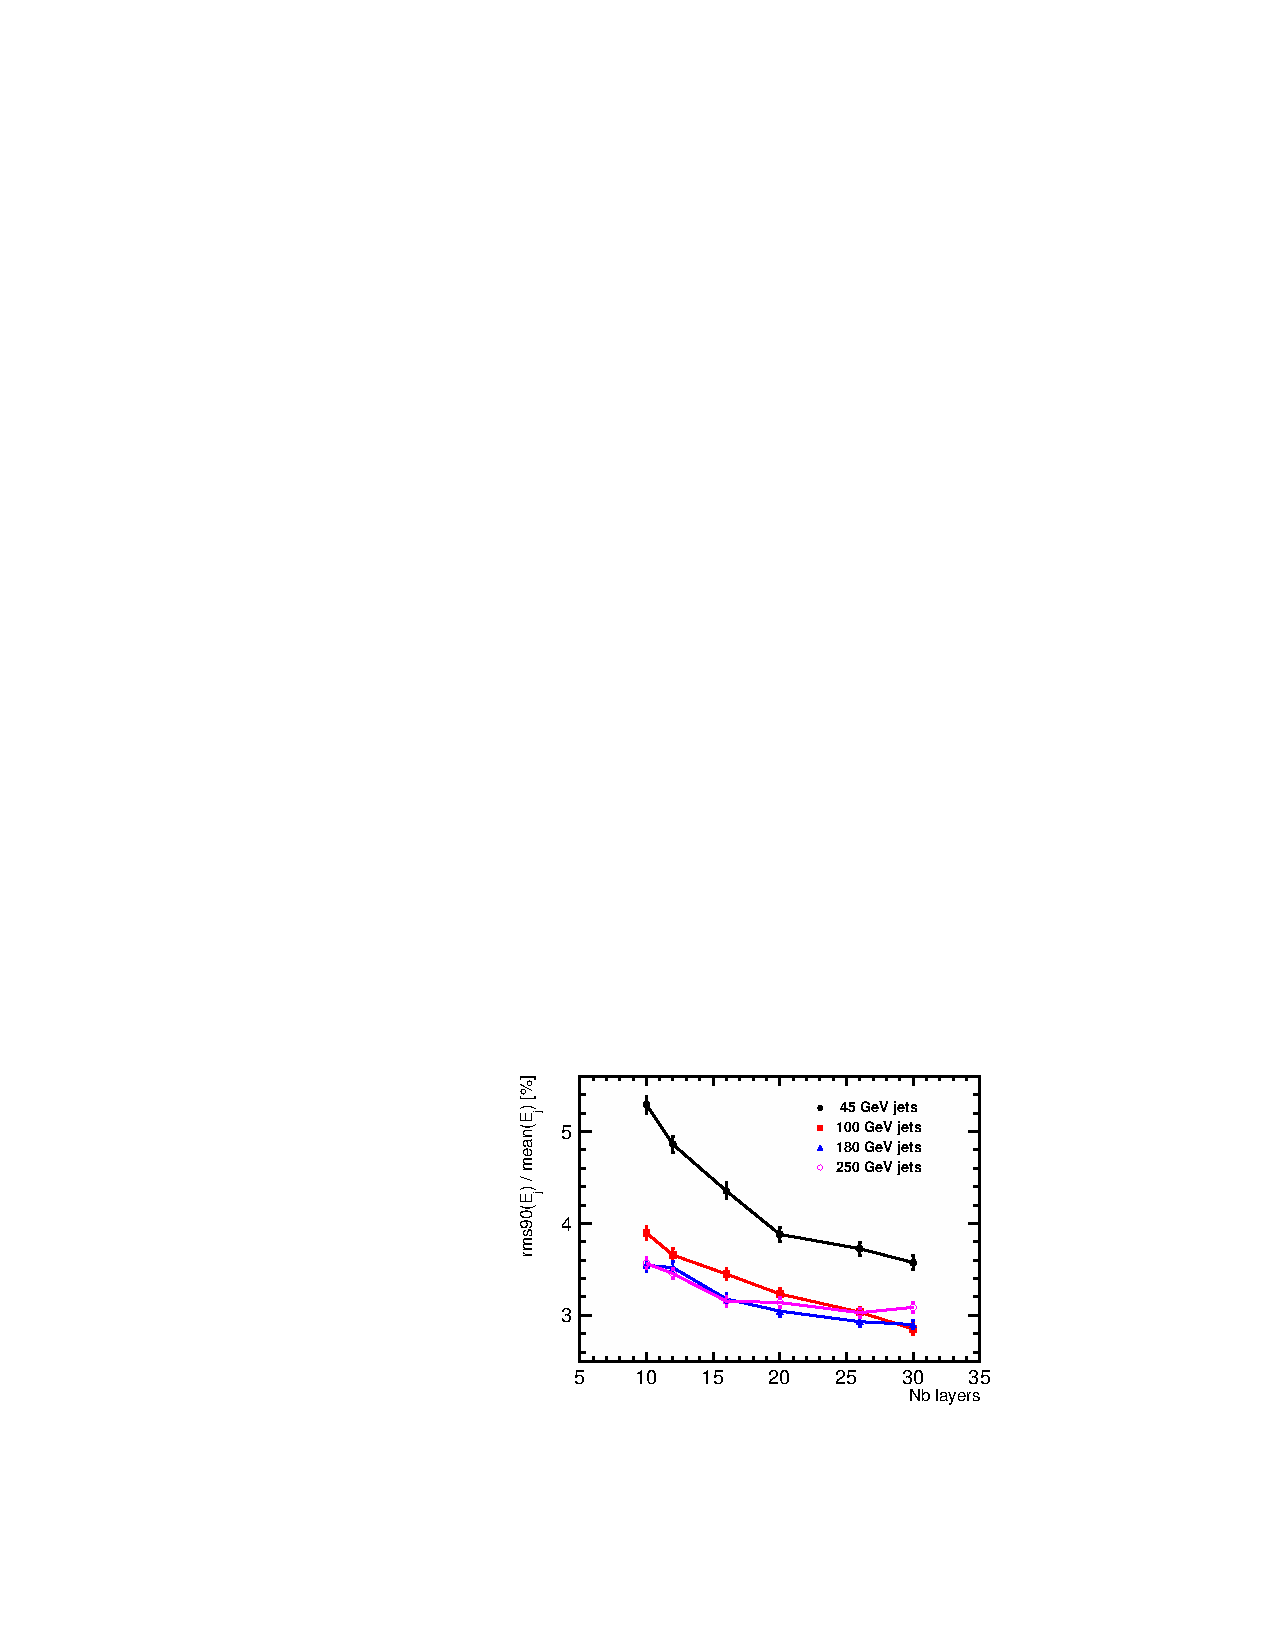
\includegraphics[width=\textwidth]{ILD/ILD_ECAL_JER}
    \caption{}
    \label{fig:detectorILDECALjer}
  \end{subfigure}

\caption
{a) a cross section through the electromagnetic calorimeter layers, and b) jet energy resolution as a function of the  total jet energy using \Zuds sample at barrel region for  optimisation of the \ECAL design as a function of the number of longitudinal layers. Both plots are  taken from \cite{Behnke:2013lya}.}
\label{fig:detectorILDECALfull}
\end{figure}

\begin{comment}
The particle flow paradigm has a large impact on the design of the electromagnetic calorimeter system.
A key requirement is the capability of the system to separate overlapping showers from each other.
A calorimeter for particle flow thus needs to be able to do pattern recognition in the shower. The
electromagnetic section has a number of tasks to fulfill. It should be able to reconstruct photons
in the presence of close-by particles. It should be able to reconstruct the detailed properties of the
shower, such as shower shape, starting point and energy to distinguish early starting electromagnetic
showers from hadronic ones. It should be noted that about half of the hadronic showers start inside
the electromagnetic calorimeter. Thus an excellent three-dimensional granularity of the device is of
utmost importance.

The transverse and longitudinal segmentation of both calorimeters has been optimised based on
detailed simulation and test beam data. It has been shown that the granularity must be of the order
of X0 in all three dimensions. This implies that a sampling calorimeter is the best option for both
ECAL and HCAL. For the ECAL the most compact design can be realised with tungsten as absorber
material. For the HCAL iron is chosen as this allows an excellent energy resolution for hadrons at
manageable granularity.
For the ECAL, silicon pad diodes lead to the highest possible compactness (and effective Moli`ere
radius) and exhibit excellent stability of calibration. As an option scintillating strips with silicon
photo-sensor readout are studied, which provide a similar effective segmentation. The two technologies
can be combined in order to reach a cost-performance optimum.

In order to have a better separation of close-by showers in the calorimeter, a system with a
small Moli`ere radius is advantageous. Further help in the separation between electromagnetic and
hadronic showers can come from a large ratio between interaction length and radiation length. A
small radiation length will move the start of the electromagnetic shower earlier in the calorimeter,
while a large interaction length will reduce the fraction of hadronic showers starting in the ECAL.

The particle flow approach requires that the calorimeters are placed inside the magnetic coil,
see Sec. 1.2. This has a major impact on the layout of the detector, and on the cost. Therefore, a
compact calorimeter is preferred in order to minimise the overall physical thickness, which in turn
reduces the size of the coil. For the ECAL tungsten is a good choice for the radiator as it is dense, and
has a large ratio of interaction length to radiation length. The final system layout is a compromise
between performance and cost. The energy resolution scales with OT, where T is the individual
absorber plate thickness, while the cost scales linearly with the surface area of the readout layers. For
ILD a solution with 30 readout layers and a thickness of the ECAL of 24X0 has been chosen as the
baseline. The optimisation of the layout is ongoing.

For a chosen pad size of 5 . 5mm2 silicon pin diodes are a good choice. They can cover large
areas, are reliable and simple to operate, allow for a thin readout layer and can operate in the 3.5 T
strong central magnetic field. While the very thin silicon layers offer excellent performance for the
tracking capabilities of the calorimeter, the energy resolution is somewhat degraded. Here a less
compact device, with a thicker readout layer, will show better performance.

The requirements on granularity, compactness and particle separation lead to the choice of a
sampling calorimeter with tungsten (radiation length X0 = 3.5 mm, Moliere Radius RM = 9 mm and
interaction length = 99 mm) as absorber material. This allows for a compact design with a depth
of roughly 24 X0 within 20 cm and, compared to e.g. lead, a better separation of electromagnetic
showers generated by near-by particles. To achieve an adequate energy resolution, the ECAL is
longitudinally segmented into 30 layers, possibly with varying tungsten thicknesses. In order to
optimise the pattern recognition performance, the active layers (either silicon diodes or scintillator)
are segmented into cells with a lateral size of 5 mm.
\end{comment}

\subsection{Hadronic Calorimeter}

The requirements of the sampling hadronic calorimeter is, again, driven by the need of the particle flow. The need of three dimensional granularity in transverse and longitudinal directions is satisfied by a sampling calorimeter.

The principal role of the \HCAL is to separate neutral hadron showers from other particles, and to measure neutral hadron energies. The neutral hadron contribution of  the jet energy is around 10\% on average. A moderate fine  granular \HCAL is a good balance between cost and performance. The chosen layout is 48 longitudinal layers with 3 by 3\,cm scintillator tiles, using an analogue read out system. The layout of a technological prototype, the "EUDET prototype"  \cite{Collaboration:2011jka} is shown in \Figure{fig:detectorAHCAL}.

The longitudinal system including the \ECAL provides about 6 radiation lengths, which is sufficient to contain the hadronic showers. The transverse cell sizes has been optimised for the best jet energy resolution. The jet energy resolution as a function of \HCAL scintillator cell size for different jet energies is shown in \Figure{fig:detectorHCALoptimise}. There is no substantial gain in the jet energy resolution for cell sizes below 3\,cm. However, the jet energy resolution degrades for cell sizes above 3\,cm. Hence 3\,cm cell size is chosen for the \HCAL design.

For the absorber material, stainless steel is chosen for mechanical and calorimetric reasons. Steel allows a self-supporting structure without auxiliary supports. Also steel has a moderate ratio of interaction length to radiation length.




\begin{figure}[tbph]
\centering
  \begin{subfigure}[b]{0.45\textwidth}
    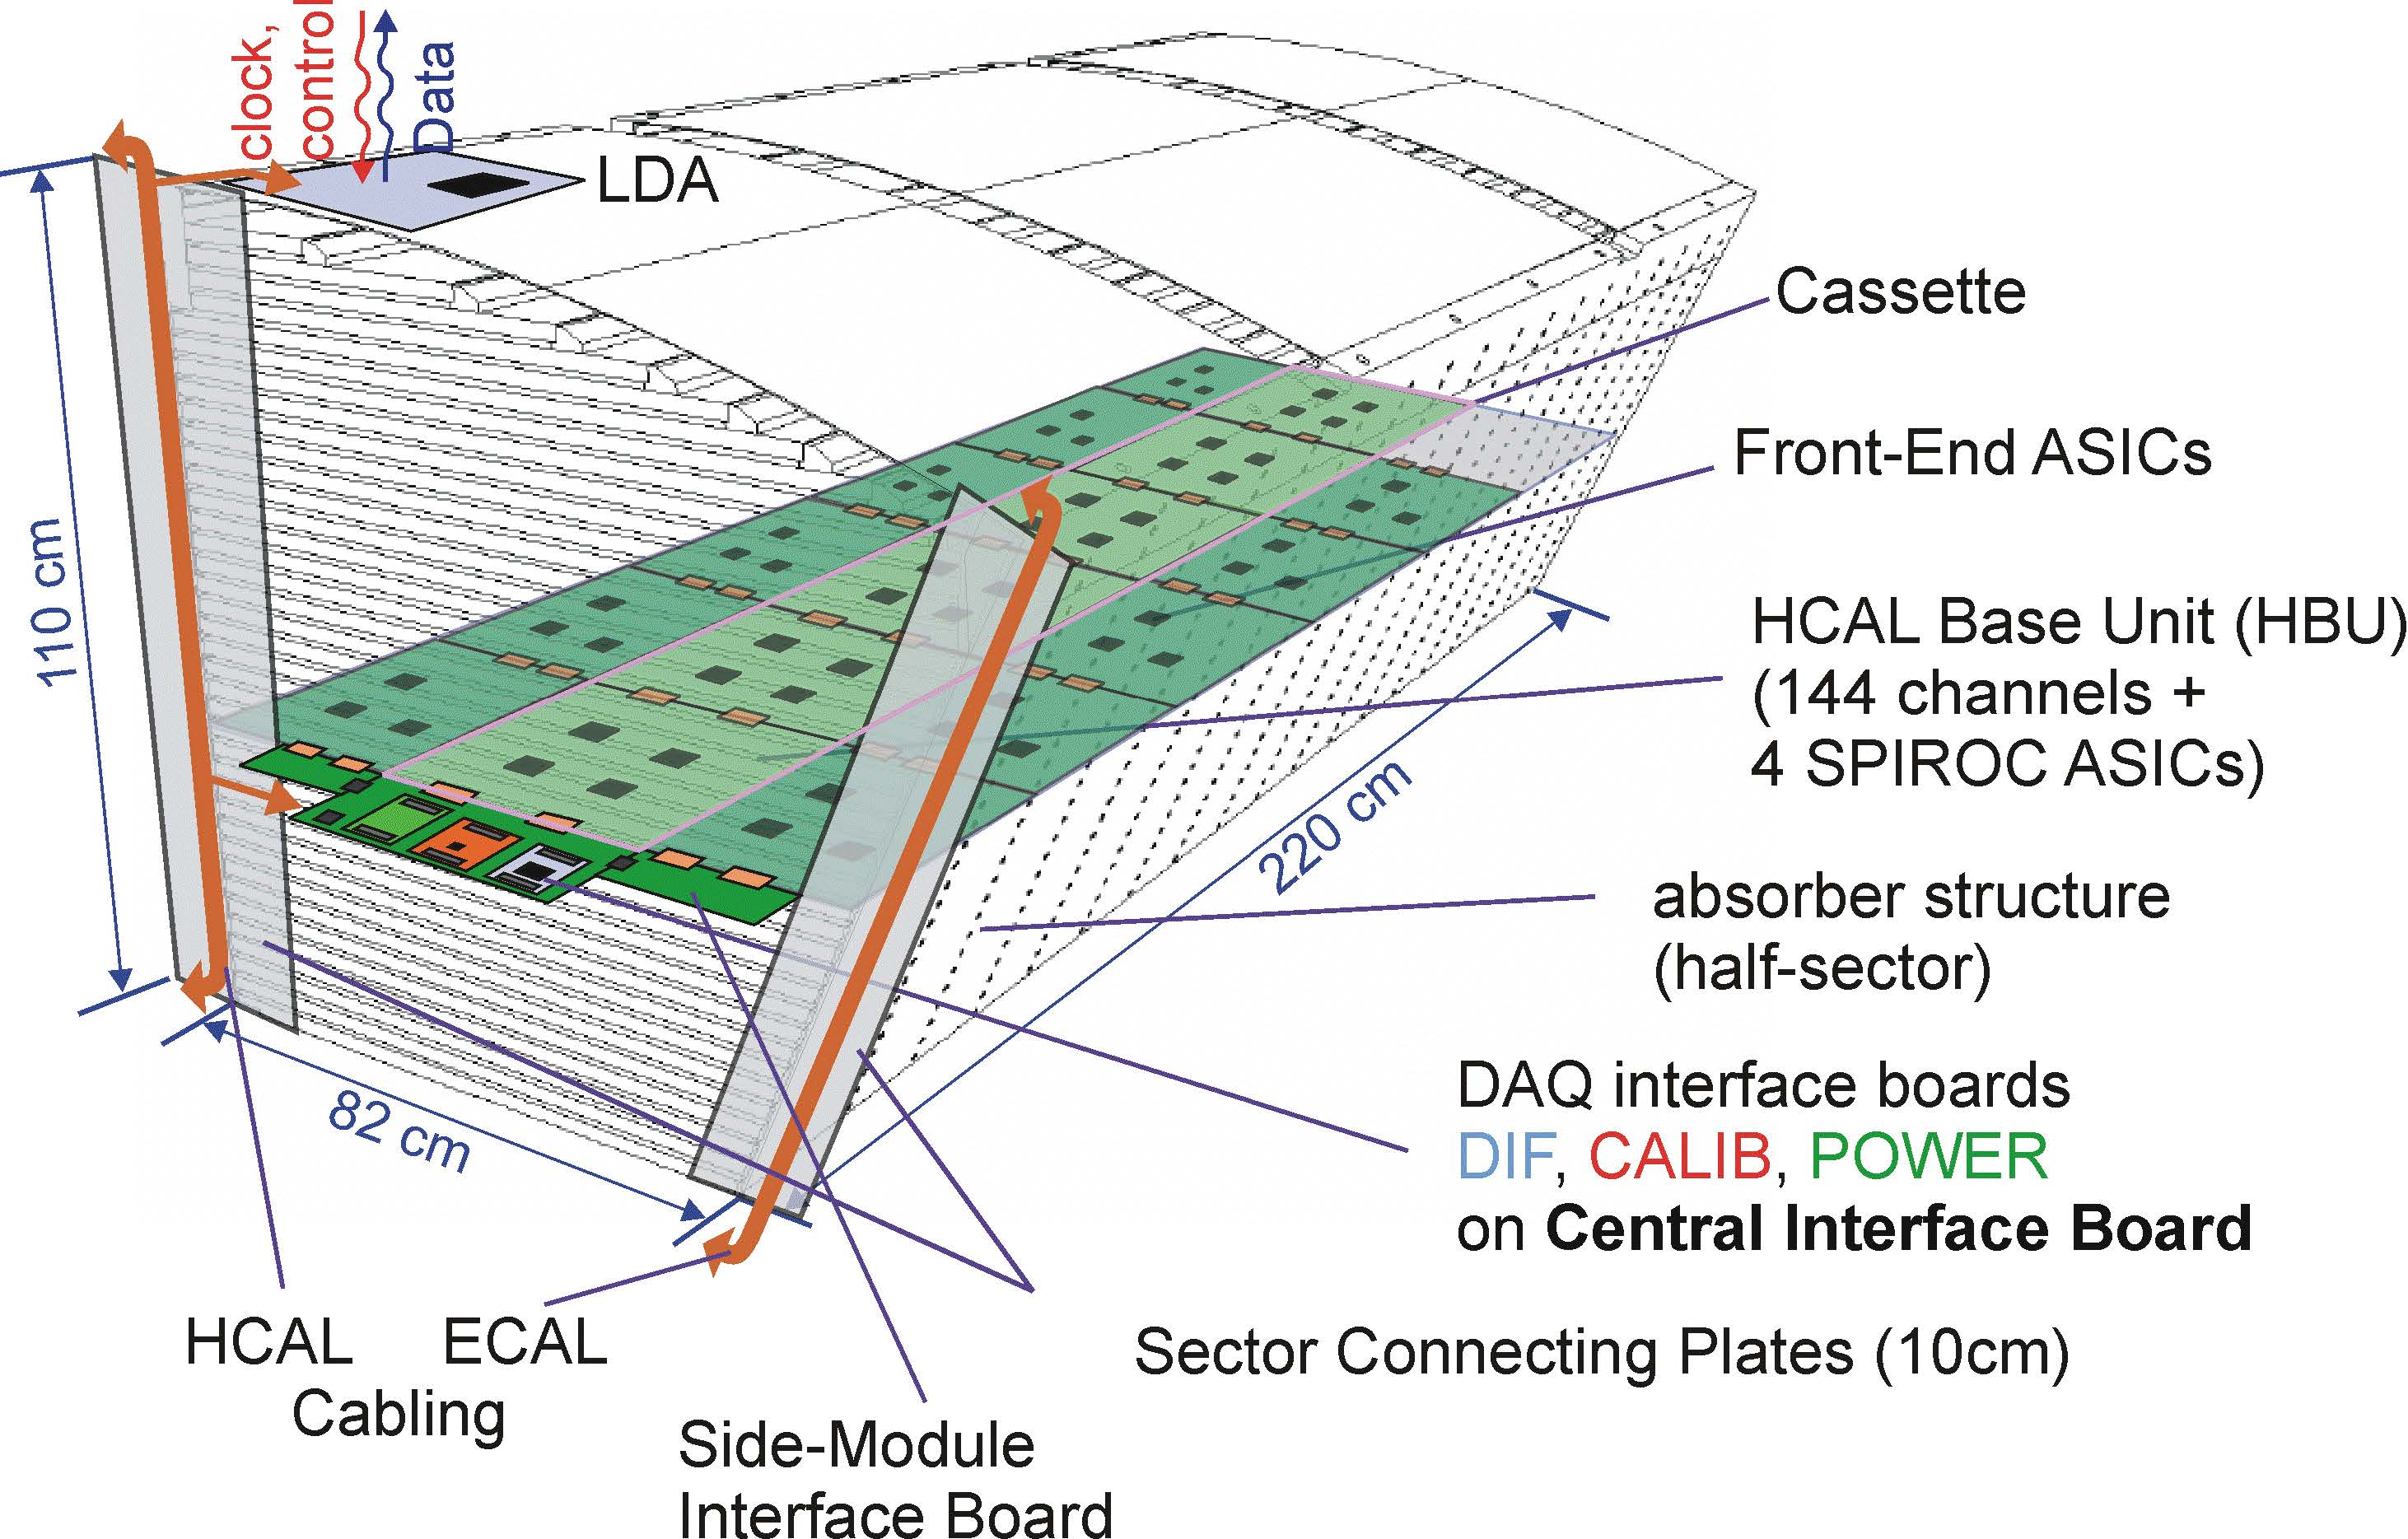
\includegraphics[width=\textwidth]{ILD/ILD_AHCAL}
    \caption{}
    \label{fig:detectorAHCAL}
  \end{subfigure}
  \begin{subfigure}[b]{0.45\textwidth}
    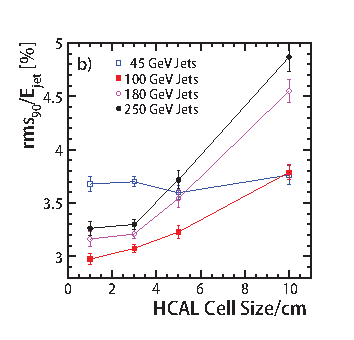
\includegraphics[width=\textwidth]{ILD/HCALoptimise}
    \caption{}
    \label{fig:detectorHCALoptimise}
  \end{subfigure}
\caption[CALICE AHCAL technological prototype module and  jet energy resolution.]
{a) the schematic view of a CALICE AHCAL technological prototype module.  b) the jet energy resolution as a function of the hadronic calorimeter scintillator cell sizes, with different energies. Both figures are taken from \cite{Baer:2013cma}.}
\label{fig:detectorHCAL}
\end{figure}


\begin{comment}
The role of the HCAL is to separate the deposits of charged and neutral hadrons and to precisely
measure the energy of the neutrals. Their contribution to the jet energy, around 10% on average,
fluctuates over a wide range from event to event, and the accuracy of the measurement is the
dominant contribution to the particle flow resolution for jet energies up to about 100 GeV. For higher
energies, the performance is dominated by confusion, and both topological pattern recognition and
energy information are important for correct track cluster assignment.


This is followed by a highly segmented hadronic calorimeter (HCAL) with up to 48 longitudinal
samples and small transverse cell size. Two options are considered, both based on a Steel-absorber
structure. One option uses scintillator tiles of 3 . 3 cm2, which are read out with an analogue
system. The second uses a gas-based readout which allows a 1.1 cm2 cell geometry with a binary or semi-digital readout of each cell.


The HCAL is optimized to measure neutral hadrons
well and thus has to provide the topological resolution power for separating them from the showers of
the much more abundant charged hadrons which must be matched with tracks.


The transverse and longitudinal segmentation of both calorimeters has been optimised based on
detailed simulation and test beam data. It has been shown that the granularity must be of the order
of X0 in all three dimensions. This implies that a sampling calorimeter is the best option for both
ECAL and HCAL. For the ECAL the most compact design can be realised with tungsten as absorber
material. For the HCAL iron is chosen as this allows an excellent energy resolution for hadrons at
manageable granularity.



The role of the HCAL is to separate the deposits of charged and neutral hadrons and to precisely
measure the energy of the neutrals. Their contribution to the jet energy, around 10% on average,
fluctuates over a wide range from event to event, and the accuracy of the measurement is the
dominant contribution to the particle flow resolution for jet energies up to about 100 GeV. For higher
energies, the performance is dominated by confusion, and both topological pattern recognition and
energy information are important for correct track cluster assignment.




The HCAL is conceived as a sampling calorimeter with steel absorber and scintillator tiles
(analogue HCAL) or gaseous devices (semi-digital HCAL) as active medium. Due to the rigidity of
stainless steel, a self-supporting structure without auxiliary supports (dead regions) can be realised.
Moreover, in contrast to heavier materials, iron with its moderate ratio of hadronic interaction length
(.I = 17 cm) to electromagnetic radiation length (X0 = 1.8 cm) allows a fine longitudinal sampling
in terms of X0 with a reasonable number of layers in a given total hadronic absorption length, thus
keeping the detector volume and readout channel count at an acceptable level. This fine sampling is
beneficial both for the measurement of the sizeable electromagnetic energy part in hadronic showers
and for the topological resolution of shower substructure, needed for particle separation and weighting.
Two baseline technology options have been developed, the scintillator-tile based AHCAL and the
Glass Resistive Plate Chamber (GRPC) based SDHCAL.
\end{comment}

\subsection{Solenoid, Yoke and Muon system}

A large superconducting solenoid outside the calorimeters produces a nominal  3.5\,T magnetic field. An iron yoke is instrumented with scintillator strips as active layers. The yoke returns the magnetic flux, and also acts as a muon detector and tail catcher calorimeter at the same time. The layout of the solenoid and the muon detector is shown in \Figure{fig:detectorILDMuon}. The maximum magnetic field at 15\,m radial distance from the detector is 50 Gauss to ensure safety \cite{Parker:21354}. A highly efficient muon detector is provided by the 3 by 3\,cm scintillator strips.  The first layer of the muon detector, also acting as a tail catcher calorimeter, catches the energy leakage from the \HCAL and the \ECAL. It has been shown that a 10\% improvement of single particle energy resolution is possible with the tail catcher \cite{CALICE:2012aa}.



\begin{figure}[tbph]
\centering
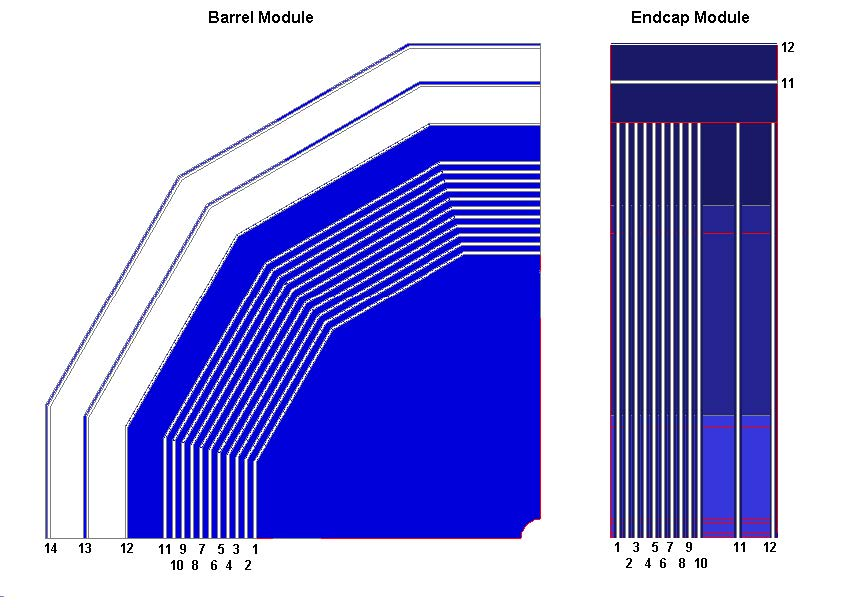
\includegraphics[width=0.45\textwidth]{ILD/ILD_Muon}
\caption
{Sensitive layers of the \ILD muon system, taken from \cite{Baer:2013cma}.}
\label{fig:detectorILDMuon}
\end{figure}

\begin{comment}
the iron Yoke has been instrumented with scintillator based active layers. At the
moment tiles with 3 . 3 cm2 granularity are used, for muon detection and serving as a tail
catcher for the HCAL; this is different than the detector baseline which uses 3 cm wide and 1
m long strips;

During beam operation the IR hall has to be accessible due to the push-pull concept. Since all
activities in a high magnetic field are very cumbersome and potentially dangerous, a field limit of 50 G
at 15 m radial distance from the beam line was agreed upon [354]. Two- and three-dimensional FEM
field calculations were done using the CST EM Studio program, varying the thickness and geometry
of the iron in the barrel and end-caps until the goal of less than 50 G at 15 m radial distance was
achieved.



An iron yoke, instrumented with scintillator strips or resistive plate chambers (RPCs), returns
the magnetic flux of the solenoid, and, at the same time, serves as a muon filter, muon detector and
tail catcher calorimeter

A stable, highly efficient muon identification system with excellent hadron rejection is an important
requirement to meet the physics goals of the ILD detector. The ILD muon system provides a number
of measurement stations outside the solenoid coil, which supplement the measurements taken with
the calorimeter system and the tracker. It is used to identify the muons and to act as a tail catcher, to
recover energy which is leaking out of the back of the calorimeter. However, the barrel part location
behind the coil limits its role to fairly high momentum particles.
The muon system/ tail catcher instruments the iron return yoke in the barrel and in the forward
region. The yoke barrel part is equipped with one sensitive layer in front of the iron yoke, 10 layers
spaced 14 cm apart, followed by three sensitive layers spaced by 60 cm apart. The forward part of the
yoke is equipped with 10 layers spaced by 14 cm, followed by two sensitive layers spaced by 60 cm.
The overall layout of the muon system/ tail catcher is shown in Figure

The first layers of the muon system serve as a tail catcher, measuring the energy which leaks through
the end of the calorimeter system. Figure III-4.5 shows the effect of an ideal tail catcher (no dead
material between the calorimeter and the tail catcher) and the realistic scenario at ILD, with two
interaction lengths of material in front of the tail catcher, as a function of the total depth of the
calorimeter system. For 6 ., the value for the ILD calorimeter system, a roughly 10% improvement is
possible with the tail catcher [348].
A prototype of the muon system/tail catcher was successfully tested during the 2007-2012
CALICE test beam campaign with ECAL and analogue HCAL. A tail catcher was placed behind the
HCAL instrumented with scintillator strips and readout with SiPMs [348]. Results from the tests
show that the proposed system delivers the anticipated performance and thus validates the technology
needed to built a muon system for ILD.
\end{comment}

\subsection{Very Forward Calorimeters}

The forward region detectors provide luminosity measurements and forward coverage of calorimeters. A system of precision and radiation resistent calorimeters are required. The luminosity calorimeter counts  Bhabha scattering to measure the luminosity to precision of $10^{-3}$ at a 500\,GeV centre-of-mass energy \cite{1748-0221-3-10-P10004}. The beam calorimeter (\BeamCAL), which is hit by many beamstrahlung pairs after each bunch corssing, extends the forward coverage. The \BeamCAL also estimates a bunch-by-bunch luminosity. An additional hadron calorimeter at the forward region, \LHCAL,  extends the angular coverage of the \HCAL to that of the \LumiCAL. Electron tagging is possible with the very forward calorimeters\cite{sailer2012radiation}, which aids event reconstruction at a high centre-of-mass energy.


\begin{figure}[tbph]
\centering
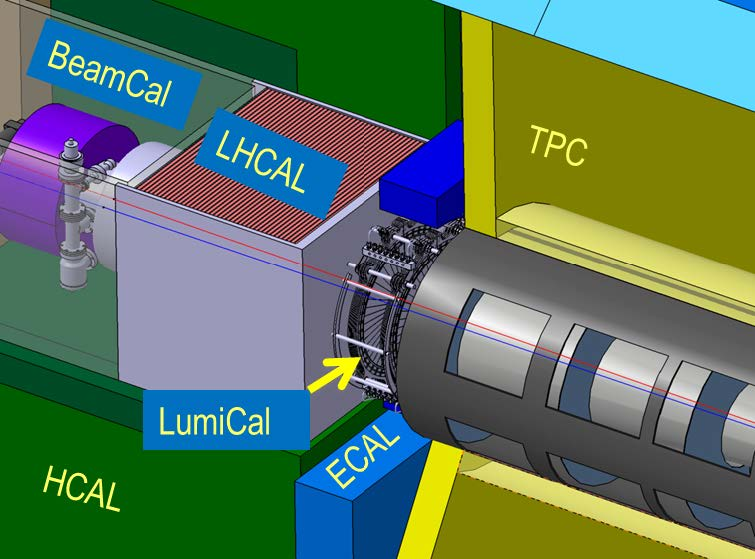
\includegraphics[width=0.45\textwidth]{ILD/ILD_forward}
\caption[The forward calorimeters of the \ILD.]
{The forward calorimeters of the \ILD, taken from \cite{Baer:2013cma}. The \LumiCAL, the \BeamCAL, and the \LHCAL are the luminosity calorimeter, the beam calorimeter, and the forward hadronic calorimeter, respectively.}
\label{fig:detectorILDForward}
\end{figure}

\begin{comment}

At very forward angles, below the coverage provided by the ECAL and the HCAL, a system of
high precision and radiation hard calorimetric detectors (LumiCAL, BeamCAL, LHCAL) is foreseen.
These extend the calorimetric coverage to almost 4fi, measure the luminosity, and monitor the quality
of the colliding beams

Two special calorimeters are foreseen in the very forward regions of the detector [324], denoted
hereafter as LumiCal and BeamCal. LumiCal will measure the luminosity with a precision of better
than 10��3 at 500 GeV centre-of-mass energy1, and BeamCal will perform a bunch-by-bunch estimate
of the luminosity and, supplemented by a pair monitor, assist beam tuning when included in a fast
feedback system [325]. Both calorimeters extend the detector coverage to low polar angles, important
e.g. for new particle searches with missing energy signature [326]. The additional low angle hadron
calorimeter LHCAL extends the coverage of the hadron calorimeter to the polar angle range of
LumiCal. A sketch of the design is shown in Figure III-3.24.
LumiCal is positioned in a circular hole of the end-cap electromagnetic calorimeter ECAL.
BeamCal is placed just in front of the final focus quadrupole. LumiCal covers polar angles between
31 and 77 mrad and BeamCal between 5 and 40 mrad.
Due to the high occupancy originating from beamstrahlung and two-photon processes, both
calorimeters need a fast readout. In addition, the lower polar angle range of BeamCal is exposed to a
large flux of low energy electrons, resulting in radiation depositions up to one MGy per year. Hence,
radiation hard sensors are needed.

\end{comment}


%This section will describe sub-systems from small to large radius.



\begin{comment}
The International Large Detector (ILD) is a concept for a detector at the International Linear Collider,
ILC [198]. In a slightly modified version, it has also been proposed for the CLIC linear collider [199].
The ILD detector concept has been optimised with a clear view on precision. In recent years
the concept of particle flow has been shown to deliver the best possible overall event reconstruction.
Particle flow implies that all particles in an event, charged and neutral, are individually reconstructed.
This requirement has a large impact on the design of the detector, and has played a central role in
the optimisation of the system. Superb tracking capabilities and outstanding detection of secondary
vertices are other important aspects. Care has been taken to design a hermetic detector, both in
terms of solid-angle coverage, but also in terms of avoiding cracks and non-uniformities in response.
The overall detector system has undergone a vigorous optimisation procedure based on extensive
simulation studies both of the performance of the subsystems, and on studies of the physics reach
of the detector. Simulations are accompanied by an extensive testing program of components and
prototypes in laboratory and test-beam experiments.
Figure III-1.1
View of the ILD detector
concept.
The ILD detector concept has been described in a number of documents in the past. Most
recently the letter of intent [198] gave a fairly in depth description of the ILD concept. The ILD
concept is based on the earlier GLD and LDC detector concepts [200, 201, 202]. Since the publication
of the letter of intent, major progress has been made in the maturity of the technologies proposed for
ILD, and their integration into a coherent detector concept
\end{comment}




\section{The \CLIC versus the \ILC}


The two main differences between the \CLIC and the \ILC are the high centre-of-mass energy and the high bunch charge density at the \CLIC, which leads to significant beam related backgrounds.  At the \CLIC, within a bunch train, there is 0.5\,ns between bunch crossings.  There are two main sources of beam induced background at the \CLIC colliding environment: incoherent electron pairs from  photon (real or virtual) interactions with individual particles of the other beam, and interactions of two photons from the colliding beams. These differences leads to a modification in the detector design and the reconstruction software for the \CLIC.



\subsection{The \CLICILD versus the \ILD}



There are two detector concepts studied in the \CLIC conceptual design report \cite{Linssen:2012hp}, the \CLICILD and the \CLICSiD. The \CLICILD detector concept is based on the \ILD design. The \CLICILD and \ILD share similarities due to similar physics motivations. Only the differences are highlighted here. A comparison of the \CLICILD and the \ILD longitudinal cross sections can be seen in \Figure{fig:detectorILD}. A comparison of key parameters of the \ILD and the \CLICILD detector concepts is shown in \Table{tab:ILDvsCLICILD}.


\begin{table}[htbp]
\centering
\smallskip
\begin{tabular}{l  r  r }
\hline
\hline
Concept &  \ILD & \CLICILD \\
\hline
Tracker & TPC/Silicon & TPC/Silicon \\
Solenoid Field (T) & 3.5 & 4 \\
Solenoid Field Bore (m) & 3.3 & 3.4 \\
Solenoid Length (m) & 8.0 & 8.3 \\
\VTX Inner Radius (mm) & 16 & 31 \\
\ECAL $r_{min}$ (m) & 1.8 & 1.8 \\
\ECAL $\Delta{r}$ (mm) & 172 & 172 \\
\HCAL Absorber B / E & Fe / Fe & Fe / W \\
\HCAL Interaction Length & 5.5 & 7.5 \\
Overall Height (m) & 14.0 & 14.0 \\
Overall Length (m) & 13.2 & 12.8 \\
\hline

\hline
\end{tabular}

\caption[A comparison of key parameters of the \ILD and \CLICILD detector concepts.]
{ A comparison of key parameters of the \ILD and \CLICILD detector concepts. \ECAL $r_{min}$ is the smallest distance from the calorimeter to the main detector axis. \HCAL Absorber B / E indicates the absorber material for the barrel (B) and the endcap (E). The table is adapted from \cite{Linssen:2012hp}.}
\label{tab:ILDvsCLICILD}
\end{table}


For the \CLICILD vertex detector, the first layer is moved outwards by 15\,mm due to a larger high occupancy region with a higher centre-of-mass energy. The detector is also required to provided time stamping at nanoseconds level, which need a different electronically component than that of the \ILD.

For the \CLICILD tracking detector, the same silicon-\TPC hybrid structure is used.  At the \CLIC, it is challenging to use a \TPC to sperate two tracks in high energy jets and to identify events in the collection of 312 bunch crossings in 156\,ns. Hence the outer silicon tracking system is important to achieve a high momentum resolution at high centre-of-mass energy. The solid angle coverage of the tracking detector is $12\degree \lesssim \theta \lesssim 168\degree$

For the \CLICILD design, the same \ECAL from the \ILD is assumed, as the requirements of a \CLIC detector are satisfied by the  \ECAL design at the \ILD. The increased centre-of-mass energy results in extra energy leakage. The leakage is controlled by the \HCAL.  And only a small fraction of particles are affected by the leakage.

For the \HCAL at the \CLICILD , extra layers are added to contain the hadronic shower at a high centre-of-mass energy. The increased thickness is justified by the simulation studies \cite{Linssen:2012hp}, where the jet energy resolution degrades quickly for a thinner \HCAL. To sustain the same inner bore radius, a more dense material, Tungsten, is chosen as the absorber material in the \HCAL barrel.

The magnetic filed is increased to 4\,T  for a better performance at a high centre-of-mass energy. Due to the different magnetic field strength, the iron yoke thickness is therefore increased to 230\,cm.

The \CLICILD adopted a similar very forward calorimetry system as that of the \ILD. The dimensions of the elements are changed due to a difference in the crossing angle (20\,mrad for the \CLIC and 14\,mrad for the \ILC). A comparison of the \LumiCAL and the \BeamCAL at the \ILD and the \CLICILD is shown in \Table{tab:detectorForwardILDvsCLICILD}.

%Modifications to the design due to the \CLIC 3\,TeV centre-mass-of energy can be found in \cite{Linssen:2012hp}.

\begin{figure}[tbph]
\centering
  \begin{subfigure}[b]{0.45\textwidth}
    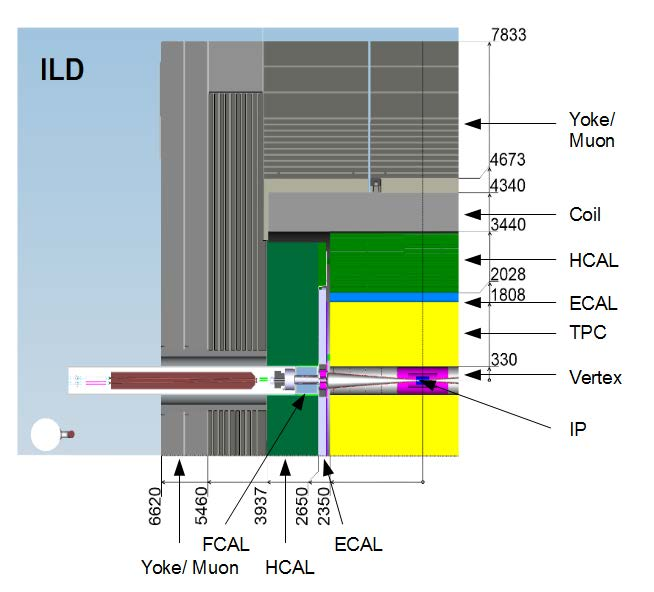
\includegraphics[width=\textwidth]{ILD/ILD}
    \caption{}
    \label{fig:ILD}
  \end{subfigure}
  \begin{subfigure}[b]{0.35\textwidth}
    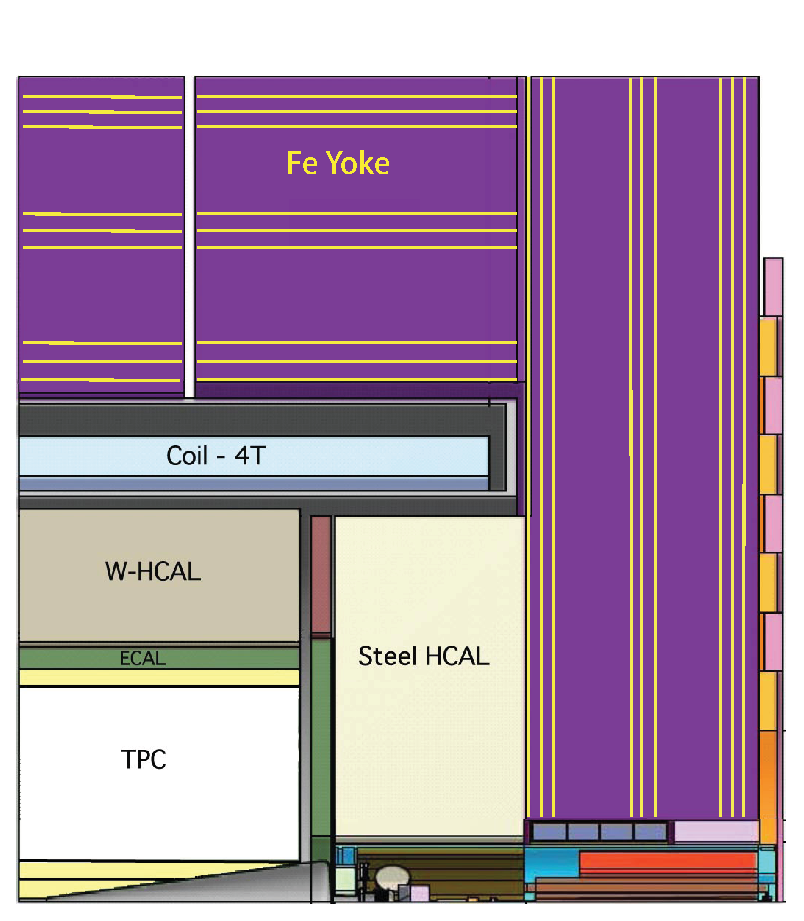
\includegraphics[width=\textwidth]{ILD/CLIC_ILD}
    \caption{}
    \label{fig:CLIC_ILD}
  \end{subfigure}
\caption[Longitudinal cross section of top quadrant of the \ILD and the \CLICILD detector concepts.]
{The longitudinal cross section of top quadrant of a) the \ILD, taken from  \cite{Baer:2013cma}, and b) the \CLICILD, taken from  and \cite{Linssen:2012hp}. For both plots, from interaction point (\IP) outwards, there is a tracking system comprising a large time projection chamber (\TPC) augmented with silicon tungsten layer, highly granular electromagnetic calorimeters (\ECAL) and hadronic calorimeters (\HCAL), muon chambers, forward calorimeters (\FCAL), magnetic coils and iron yokes. The numbers are in units of mm.}
\label{fig:detectorILD}
\end{figure}



\begin{table}[htbp]
\centering
\smallskip
\begin{tabular}{l l r  r }
\hline
\hline
 & &  \ILD & \CLICILD \\
\hline
\LumiCAL & geometrical acceptance (mrad)& 31 - 77 & 38 - 110 \\
& fiducial acceptance (mrad) & 41 - 67 & 44 - 80 \\
& z (start) (mm) & 2450 & 2654 \\
& number of layers (W + Si) & 30 & 40 \\
\hline
\BeamCAL & geometrical acceptance (mrad)& 5 - 40 & 10 - 40 \\
& z (start) (mm) & 3600 & 3281 \\
& number of layers (W + sensor) & 30 & 40 \\
& graphite layer thickness (mm) & 100 & 100 \\
\hline
\hline
\end{tabular}
\caption[Comparison of the \LumiCAL and the \BeamCAL at the \ILD and the \CLICILD .]%
{Comparison of the key parameters of the \LumiCAL and the \BeamCAL at the \ILD and the \CLICILD . The table is adapted from \cite{Linssen:2012hp}. }
\label{tab:detectorForwardILDvsCLICILD}
\end{table}

%Beam Calorimeter acceptance is defined as \absCosTheta is between  0.01 and 0.04\,rad and length in z direction is between 3181 and 3441\,mm. Luminosity Calorimeter acceptance is defined as \absCosTheta is between  0.038 and 0.11\,rad and length in z direction is between 2539 and 2714\,mm.




  \chapter{Simulation, reconstruction and analysis software}
\label{chap:Reconstruction}

\chapterquote{All the world's a stage, And all the men and women merely players; They have their exits and their entrances, And one man in his time plays many parts.}%
{William Shakespeare, 1564 - 1616}%: Blackwood's Magazine May 1830

%As previously stated, this document focus on the \ILD and \CLICILD detectors. Due to the similarity, we often only discuss one detector to avoid the repetition. The difference in detectors will be stated if applicable.

In previous chapters, overviews of the theory and the future linear collider experiments have been described. In this chapter simulation, reconstruction and analysis software are discussed. Automated analysis is the only way to deal with the vast amount of data generated in high energy physics. Hence the software supporting the automated analysis are important. An analysis often consists of  monte carlo event generations, event reconstructions, and using software to extract information of the event. Hence they are discussed together in this chapter.

Simulation and reconstruction of events of the future Linear Colliders, \ILC and \CLIC, share a  common software framework.  Therefore,  the shared simulation and  reconstruction software is discussed first, and the \CLIC specific issues are highlighted afterwards. The event reconstruction focuses on the \pandora event reconstruction, which is the framework for the photon reconstruction algorithms in \Chapter{chap:Photon}. Lastly analysis software is presented.   The multivariate analysis  is discussed  in lengthy details due to its complexity.

\section{Monte Carlo event generation}
\label{sec:pandoraMC}
Monte Carlo (MC) event generation is often the first step for the simulated study. Most events used in this thesis are generated with the WHIZARD software \cite{whizard,Moretti:2001zz}. Some simple events used in this thesis are generated by writing the event manually in the  HEPEVT format \cite{Altarelli:1989hx}. The PYTHIA software \cite{Sjostrand:1995iq} is used to describe parton showering, hadronisation and fragmentation. The parameters for the PYTHIA are tuned to OPAL data from the Large Electron-Positron collider (LEp) \cite{Alexander:1995bk}. The TAUOLA software \cite{Jadach:1993hs} describes the tau lepton decay with correct spin correlations of the decay products. The Initial State Radiation (\ISR) effect is simulated in the WHIZARD, with the \ISR photons being collinear with the beam direction. The Final State Radiation (\FSR) is simulated in the PYTHIA.


%, with no polarisation of the electron and positrons.

\section{Event Simulation}

For all the simulated events used in this thesis, the simulation software used to simulate the interaction of particles through the detector material is the GEANT4 software \cite{Agostinelli:2002hh}. The detector geometry description is provided by the MOKKA software \cite{MoradeFreitas:2002kj}.  The QGSP\_BERT physics list is used to describe the hadronic shower decay in the detector.

%The  QGSP\_BERT physics list uses the Bertini model \cite{Proceedings:2003lxa} at low energies, making a transition to the Low Energy Parameterisations (GHEISHA \cite{TechnicalReportPITHA 85-02}) model between 9.5 and 9.9\,GeV, and a further transition to the QGSP model between 12 and 25\,GeV.  QGSP model is a GEANT4 implementation of a string model~\cite PhysRevLett.67.1523 for the high energy interaction, supplemented by the  GEANT4} precompound model\cite{mazzucato2001proceedings}

\section{Event Reconstruction}

With simulated events (or real data in the future) as inputs, the next step is to reconstruct these events. The reconstruction software runs in the Marlin framework \cite{Gaede:2006pj}, as a part of the \ilcsoft software package. The event reconstruction contains following steps: digitisation of simulated calorimeter hits, reconstruction of tracks in the tracking system (using pattern recognition algorithms), and particle flow objects (\PFOs) reconstruction with \pandora\cite{Thomson:2009rp,Marshall:2012ry}. Details of the reconstruction can be found in \cite{Brau:2007zza,Linssen:2012hp}. Here particle flow reconstruction via \pandora will be discussed in details, as \pandora provides the software framework for the photon reconstructions in \pandora in \Chapter{chap:Photon} and is used in \Chapter{chap:Tau} and \Chapter{chap:DoubleHiggs}.

\section{\pandora event reconstruction}
\label{sec:pandoraPandoraPFA}

The tradition energy flow approach to calorimetry is unable to meet the mass and energy resolution requirements for future linear colliders. The particle flow approach to calorimetry with \pandora has a proof-of-principle demonstration of its capability to reach the required resolution. The particle flow approach also put stringent requirements on the detector design, which is described in \Section{sec:detectorPhysicsRequirementPandora}. By associating calorimeter hits to the tracks, around 60\% of the jet energy from charged particles is measured by the tracker, which has a much better resolution than the calorimeter. Small cell sizes of the calorimeters are required to identify hits from different particles. The traditional sum of calorimeter cell energies is replaced by particle flow reconstruction algorithms - a complex pattern recognition problem.  The \pandora algorithm has been developed and used in the \ILC and \CLIC simulation studies. There are over 60 linear collider specific reconstruction algorithms. Each aims to address a particular topological issue in the reconstruction.

Developed with the \ILD detector concept, \pandora has been adapted to the \CLIC condition and shows its ability to deliver required energy resolutions \cite{Linssen:2012hp}.  In the recent development, the core base codes for basic object and memory managements are factorised in the Pandora C++ Software Development Kit\cite{Marshall:2015rfa}.
% Recent the code base of the \pandora has been restructured.
In the subsequent sections, the main steps in the \pandora reconstructions are described. The details of the reconstruction can be found in \cite{Thomson:2009rp,Marshall:2012ry,Marshall:2015rfa}. The inputs of \pandora are digitised calorimeter hits and reconstructed tracks, with some detector geometry information to aid the reconstruction. The output are reconstructed particles with four-momenta, also known as the Particle Flow Objects (\PFOs).

\subsection{Track selection}
\label{sec:pandoraPandoraTrack}

Tracks from the inner tracking detectors are important inputs of the \pandora reconstruction. These tracks are selected based on their topological properties, how likely they are from physical processes, and whether they are consistent with the tracker resolution. Only tracks passing the selection are used for the subsequent reconstruction.

Special topologies of tracks are identified, such as when a neutral particle decays or converts into a pair of charged tracks, leaving tracks of a ``V0''  shape. This is identified by searching for a pair of tracks originated from a single point. Another topology is the ``kinks'' when a charged particle decays to a single charged particles with neutral particles. The last special topology are  the ``prongs'' when a charged particle decays to multiple charged particles. This information is stored and passed on to the subsequent reconstruction, along side with helical track fit (using last 50 reconstructed tracker hits) and the track projection to the front of the \ECAL.

\subsection{Calorimeter selection}

The other important inputs of  the \pandora reconstruction are the calorimeter hits from calorimeters. The properties of a calorimeter hit include the position, its layer in the calorimeter, and its energy response from the calorimeter digitiser.

Calorimeter hits are selected based on a series of criterion. The selected hits need to have energies above certain thresholds, measured in minimum ionising particle (MIP) equivalent or measured in directly converted energy. Similar to tracks, only calorimeter hits that pass the selection are used in later steps.

Extra information about calorimeter hits are calculated, stored and to be used in the later steps. The information includes the geometry information of the hit and likelihood of the hit originated from a minimum ionising particle (MIP).

Isolated hits, often originating from low energy neutrons in a hadronic shower, are difficult to associate to the correct hadronic shower. They are identified and not used during the clustering stage. However, these isolated hits participate in the reconstruction during the  last step, particle flow object (PFO) creation, to contribute to the energy estimation.


\subsection{Particle Identification}
\label{sec:particleID}

To improve the reconstruction of the charged particles, where calorimeter hits are associated to tracks, dedicated particle identification algorithms identify muons and photons and remove identified particles from the reconstruction. By removing the hits from muons and photons, the reconstruction of charged particles is improved as fewer hits are left to be reconstructed. Hence the pattern recognition problem is reduced. Identified muons and photons do not participate in the later clustering and re-clustering stages, but re-enter the reconstruction at the fragment removal stage (see \Section{sec:pandoraFragmentRemoval}). The details of the photon reconstruction algorithms and photon related algorithms are described in \Chapter{chap:Photon}.
%Dedicated particle identification algorithms aim to identify muons and photons before associating calorimeter hits to tracks.


\subsection{Clustering}
\label{sec:pandoraConeCluster}

A cone clustering algorithm is used to group calorimeter hits from innermost to outmost pseduo-layer. The output \clusters are further processed, merged or split based on their topological properties. Since the cone clustering algorithm widely used in many reconstruction algorithms in the \pandora, it is necessary to introduce the cone based clustering algorithm, before discussing the rest of the \pandora reconstruction.



\begin{figure}[tbph]
\centering
{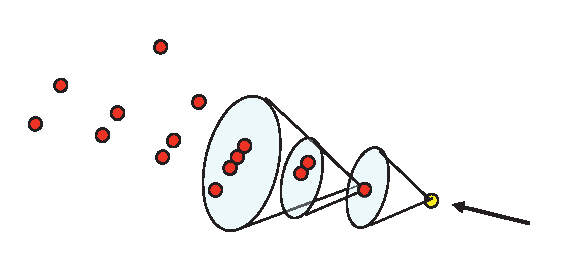
\includegraphics[width=0.5\textwidth]{pandora/coneClustering}}%
\caption{Illustration of the cone based clustering, taken from \cite{Marshall:pandoraLC}}
\label{fig:pandoraConeClustering}
\end{figure}

In general there are two main types of clustering algorithms: cone based algorithms and sequential combination algorithms(see \Section{sec:pandoraJetAlg}). The main clustering scheme used in the  \pandora is the cone based algorithms. The clustering algorithm forms clusters to group calorimeter hits. Illustrated in \Figure{fig:pandoraConeClustering}, cone clustering algorithm identifies a seed first, shown as the yellow dot. The algorithm then forms a cone to include hits that are within a specified opening angle to the seed hit. The cone based clustering algorithm is preferred because the direction of particle flow is largely unchanged from the originated particle, whether the particle flow is an electromagnetic shower, QCD radiation, or hadronisation.

%these cone clusters have similar direction and energy to the originated particle. Therefore it is applicable to use cone based clustering algorithms for building clusters.

\begin{figure}[tbph]
\centering
{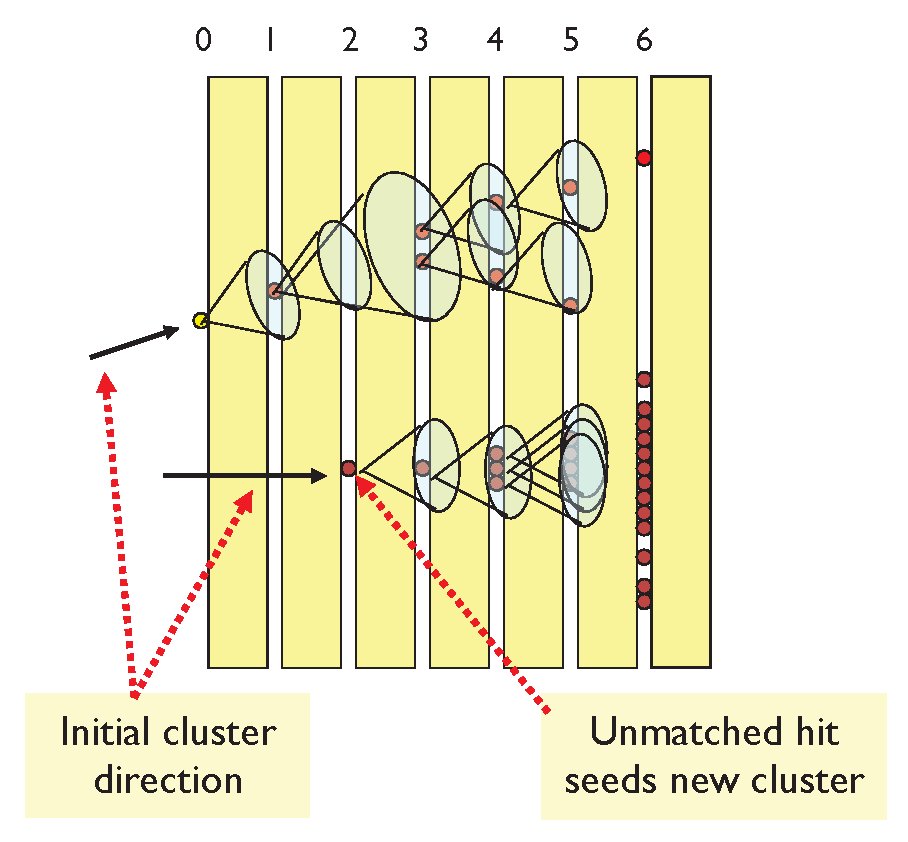
\includegraphics[width=0.5\textwidth]{pandora/coneClustering2}}%
\caption{Illustration of the clustering algorithm used  in the \pandora, taken from \cite{Marshall:pandoraLC}}
\label{fig:pandoraConeClustering2}
\end{figure}

\FIGURE{fig:pandoraConeClustering2} shows the clustering algorithm used in the \pandora. The seed for the cone clustering is typically the projection of a energetic track to the front of the \ECAL. A high  energy calorimeter hit can also be used as a seed. The initial cluster direction is taken as the direction of the seed. Afterwards, a cone with a specified opening angle and depth will be formed around the seed. The \fourMomentum of calorimeter hits are therefore summed to obtain the cone's \fourMomentum. The building of the cone is iterated from the inner layer of the \ECAL to the outer layer. At each layer, possible associations with hits in previous layers and the same layer are checked. If a hit is not associated with the cone, the hit is used to seed a new cluster. The clustering algorithm produces basic working objects, \clusters.

\subsection{Topological cluster association}

After the initial clustering, clusters are further refined using topological information. This step is necessary because the initial clustering scheme is tends to form small clusters. These small clusters are then merged  based on clear topological signatures. The merging signatures include combining track segments, connecting a track segment with gaps, connecting track segments to  hadronic showers, and merging clusters when they are within close proximity. Some association algorithms are shown schematically in \Figure{fig:pandoraTopoAsso}.  \FIGURE{fig:pandoraTopoAssoLoopTrack}, \Figure{fig:pandoraTopoAssoBackScattered}, and \Figure{fig:pandoraTopoAssoConeAsso} show rules for looping track segments, back-scattered tracks from hadronic showers, and cone association, respectively. In each case, the arrow indicates the tracks. The dark red dots represent the calorimeter hits in the associated cluster. The slightly fainter red dots represent the calorimeter hits in the neutral cluster. The black line represents the front of the \ECAL.

\begin{figure}[tbph]
\centering
  \begin{subfigure}[b]{0.3\textwidth}
    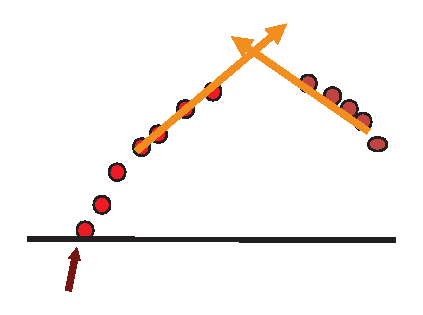
\includegraphics[width=\textwidth]{pandora/loopTrack}
    \caption{}
    \label{fig:pandoraTopoAssoLoopTrack}
  \end{subfigure}
  \begin{subfigure}[b]{0.3\textwidth}
    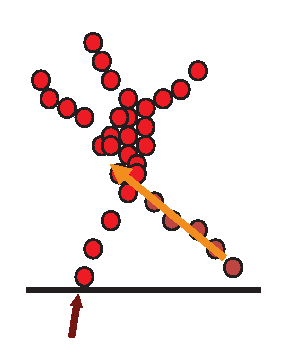
\includegraphics[width=\textwidth]{pandora/backScattered}
    \caption{}
    \label{fig:pandoraTopoAssoBackScattered}
  \end{subfigure}
  \begin{subfigure}[b]{0.3\textwidth}
    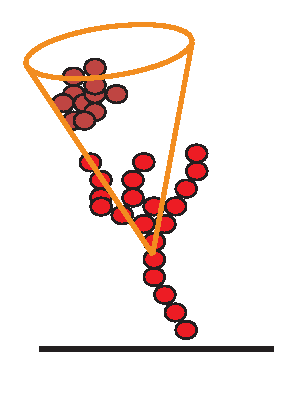
\includegraphics[width=\textwidth]{pandora/coneAsso}
    \caption{}
    \label{fig:pandoraTopoAssoConeAsso}
  \end{subfigure}
\caption[Topological association in the \pandora.]
{Examples of topological association in the \pandora. \FIGURE{fig:pandoraTopoAssoLoopTrack}, \Figure{fig:pandoraTopoAssoBackScattered}, and \Figure{fig:pandoraTopoAssoConeAsso} show rules for looping track segments, back-scattered tracks from hadronic showers, and cone association, respectively. In each case, the arrow indicates the tracks. The dark red dots represent the calorimeter hits in the associated cluster. The slightly fainter red dots represent the calorimeter hits in the neutral cluster. The black line represents the front of the \ECAL. The figures are taken from \cite{Marshall:pandoraLC}.}
\label{fig:pandoraTopoAsso}
\end{figure}

\subsection{Track-cluster association}

Having refined the clusters in the calorimeter, the next step is to connect the clusters to the tracks from the inner tracking detector. The clusters are associated to tracks, according to the proximity of the first layer of the cluster and the track projection to the front of the \ECAL. The consistency between track and initial cluster directions, as well as a match between track momentum and cluster energy, are required.


\subsection{Re-clustering}

The cluster association scheme described in the previous section works well for low energy (less than 50\,GeV) jet. For a high energy jet, particles and the subsequent hadronic showers are more boosted and more likely to overlap each other. Therefore, it is important to re-cluster based on the compatibility of the cluster energy and the associated track momentum.

The re-clustering is performed on a statistical basis. If the cluster energy and the associated track momentum do not match, the cluster will be re-clustered using the same clustering algorithm with different parameters, or differen cluster algorithms. Afterwards, out of many clusters obtained with the re-clustering step, the cluster that matches the best with the track momentum is chosen, and the cluster will be associated with that track. A schematic diagram of the re-clustering stage is shown in \Figure{fig:pandoraRecluster}. In the figure, the black upright arrows indicate the tracks. The dark red dots represent the calorimeter hits in the associated cluster. The  slightly fainter red  dots represent the calorimeter hits in the neutral cluster. In this example, the cluster energy is less than the associated track momentum. The topological association algorithms did not add the natural cluster, as it would have formed a cluster with too much energy. The re-clustering scheme tries different cone clustering by splitting the neutral cluster so that the topological association could make correct association.


\begin{figure}[tbph]
\centering
{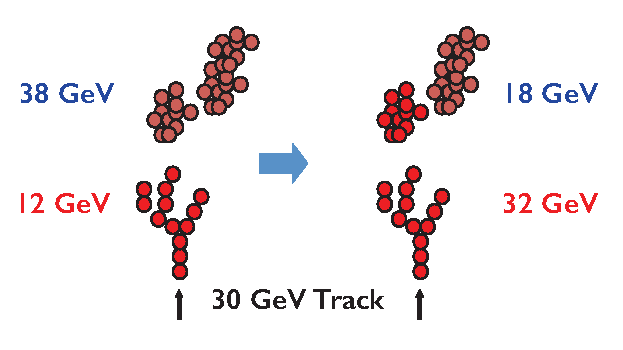
\includegraphics[width=0.6\textwidth]{pandora/recluster}}%
\caption[Illustration of the re-clustering algorithm in \pandora]
{Illustration of the re-clustering algorithm in \pandora, taken from \cite{Marshall:pandoraLC}. The arrow indicates the tracks. The dark red dots represent the calorimeter hits in the associated cluster. The  slightly fainter red  dots represent the calorimeter hits in the neutral cluster. The cluster energy is less than the associated track momentum. The topological association algorithms did not add the natural cluster, as it would have formed a cluster with too much energy. The re-clustering algorithm tries different cone clustering to split the neutral cluster so that the topological association could make correct association.}
\label{fig:pandoraRecluster}
\end{figure}

\begin{comment}
\subsection{Photon identification}

The neutral clusters are tested against an expected photon electromagnetic shower profile. The longitudinal shower profile for a photon cluster is required to be similar to a expected electromagnetic shower profile, with the discrepancy being smaller than a threshold.
\end{comment}

\subsection{Fragment removal}
\label{sec:pandoraFragmentRemoval}

This stage of the reconstruction will focus on merging low energy clusters. These neutral clusters are likely to be fragments of other clusters. The merging criterion are mostly based on the proximity and the energy comparison. Algorithms dealing with photon fragment merging and photon splitting are described in details in \Chapter{chap:Photon}.

\subsection{Particle Flow Object Creation}
\label{sec:pandoraPFOcreation}

% double counting taking care in pandora
The last stage of the reconstruction is the creation of the output objects, Particle Flow Objects (PFOs). The PFOs contain clusters and associated tracks. Simple, but effective, particle identification for electrons and muons are applied. Photon identifications are  applied at various stages of the reconstruction.

The \PFOs contain information on positions, four-momenta and associated quantities. These \PFOs are  used heavily in physics analyses. The electron, muon and photon identifications are  also used in physics analyses in \Chapter{chap:Tau} and in \Chapter{chap:DoubleHiggs}.


\section{The \CLIC specific simulation and reconstruction}

There are a few  simulation and reconstruction issues specific to the \CLIC, which affect the analysis in \Chapter{chap:DoubleHiggs}. One issue is that the luminosity spectrum for  interactions with photon from Beamstrahlung is different to electron-positron interactions. Therefore a solution is presented in \Section{sec:pandoraCLUClumi} to correct for the differences. Another issue is that there is a large amount of beam induced background in \CLIC, which needs to be suppressed before physics analyses. The background suppression is described in \Section{sec:pandoraggHad}. Lastly simulated masses of particles are given in \Table{tab:pandoraCLICparticleMass}, which will be used in \Section{sec:doubleHiggsJetOptimisation}.

%One issue is that the event reconstruction does not include calorimeters hits in the forward calorimeters due to computational reasons. Instead, a fast simulation using MC particles is used and details are laid out in \Section{sec:doubleHiggsForwardElectron}.




\subsection{Luminosity spectrum}
\label{sec:pandoraCLUClumi}

The electron-photon interaction, where the photon is produced from initial state radiation via Beamstrahlung ,  has a different  instantaneous luminosity than the electron-positron interaction. Hence, for the same time-frame, the total integrated luminosity of the electron-photon interaction is different to that of the electron-positron interaction. To correct for the difference in the luminosity, a simulated study \cite{Sailer:lumi} was performed with the GUINEAPIG \cite{Schulte:1999tx} and was simulated in the WHIZARD, to identify the ratio of the integrated luminosity of the  electron-photon interaction to the electron-positron interaction.  The results are summarised in \Table{tab:reconstrcutionBSlumi}. For the physics analysis in \Chapter{chap:DoubleHiggs}, event number for processes with initial-state photons from Beamstrahlung are corrected with the ratios in \Table{tab:reconstrcutionBSlumi}.

\begin{table}[htbp]
\centering
\smallskip
\begin{tabular}{l r  r }
\hline
Luminosity ratio &  \rootS{1.4} & \rootS{3} \\
\hline
\textit{L(\ee) / L(\ee)} &1 & 1\\
\textit{L(\Egamma) / L(\ee)} &0.75 & 0.79\\
\textit{L(\gammae) / L(\ee)} &0.75 & 0.79\\
\textit{L(\Gammagamma) / L(\ee)} &0.64 & 0.69\\
\hline
\hline
\end{tabular}
\caption[Luminosity ratio for processes with initial-state photons from Beamstrahlung.]%
{Luminosity ratio for processes with initial-state photons from Beamstrahlung at the \CLIC, at \rootS{1.4} and 3\,TeV. The table summarises results from \cite{Sailer:lumi}. }
\label{tab:reconstrcutionBSlumi}
\end{table}

\subsection{Beam induced backgrounds}
\label{sec:pandoraggHad}

The other issue considered when using the \CLICILD detector concept is the beam induced background. At high \sqrtS, the background becomes important for the event reconstruction. Therefore, the beam induced background are considered in the simulation.

There are different types of the beam induced background. The dominant one, \ggHad, intergraded over 60 bunch crossing,  is overlayed onto the reconstruction. The \ggHad is the dominant background in all calorimeters except inner part of the \HCAL endcap. Another type of the background, the incoherent pairs,  are ignored.

These \ggHad background events are hadronised with the PYTHIA, and superimposed on the physics process simulations to save computational resources. The choice of 60 bunch crossings is a conservative estimate  of  the amount of background in the experiment condition\cite{Barklow:1443518,Barklow:1443518}.

The beam induced background deposits significant amounts of energies in the detector. It needs to be suppressed for physics analyses, like the one in \Chapter{chap:DoubleHiggs}. Two software have been developed to suppress these background: a track selector and a PFO selector\cite{Marshall:2012ry}.

The track selector aims to remove poor quality and fake tracks that are more likely from the beam induced background. It places a simple track-quality cut and a time-of-arrival cut on tracks. If the arrival time of the track at the front of the \ECAL, using the helical fit, differs more than 50\,ns from using a straight line fit, the track will be rejected.


The PFO selector discards PFOs that are originated from the beam induced background, based on the transverse momentum (\pT) and time information of the PFOs. The PFOs from \ggHad often have low \pT and have a range of time-of-arrivals. In contrast, the PFOs from physics processes have a range of \pT, and the time-of-arrivals are close to the brunch crossing time. By utilising the high spatial resolution from the high granular calorimeter, individual PFOs can be tracked and reconstructed. The PFO selector uses different \pT and time cuts for the central part of the detector and for the forward part of the detector. There are different cuts for photons, neutral PFOs, and charged PFOs. Three configurations of these cuts are developed, namely ``loose'', ``normal'', and ``tight'' selections. As the name suggested, ``loose'' selection corresponds to a looser cut of \pT and time-of-arrival, allows a larger value of \pT and time-of-arrival. The optimal configuration depends on the \sqrtS of the collision, and the physics process to study. \FIGURE{fig:pandoraEvtDisplayggHad} shows the effect of the suppression of the background with the tight \PFO selection. Reconstructed particles for a time window of 10\,ns (100 \,ns in \HCAL barrel) in a simulated \HepProcess{\Pep\Pem \to \PHiggs\PHiggs \to \Ptop\APbottom\Pbottom\APtop} event in the \CLICILD dectro, with 60 bunch crossings of \ggHad background overlaid in \Figure{fig:pandoraEvtDisplayggHad1}. The effect of applying tight \PFO section cuts is shown in \Figure{fig:pandoraEvtDisplayggHad2}.


\begin{figure}[tbph]
\centering
  \begin{subfigure}[b]{0.45\textwidth}
    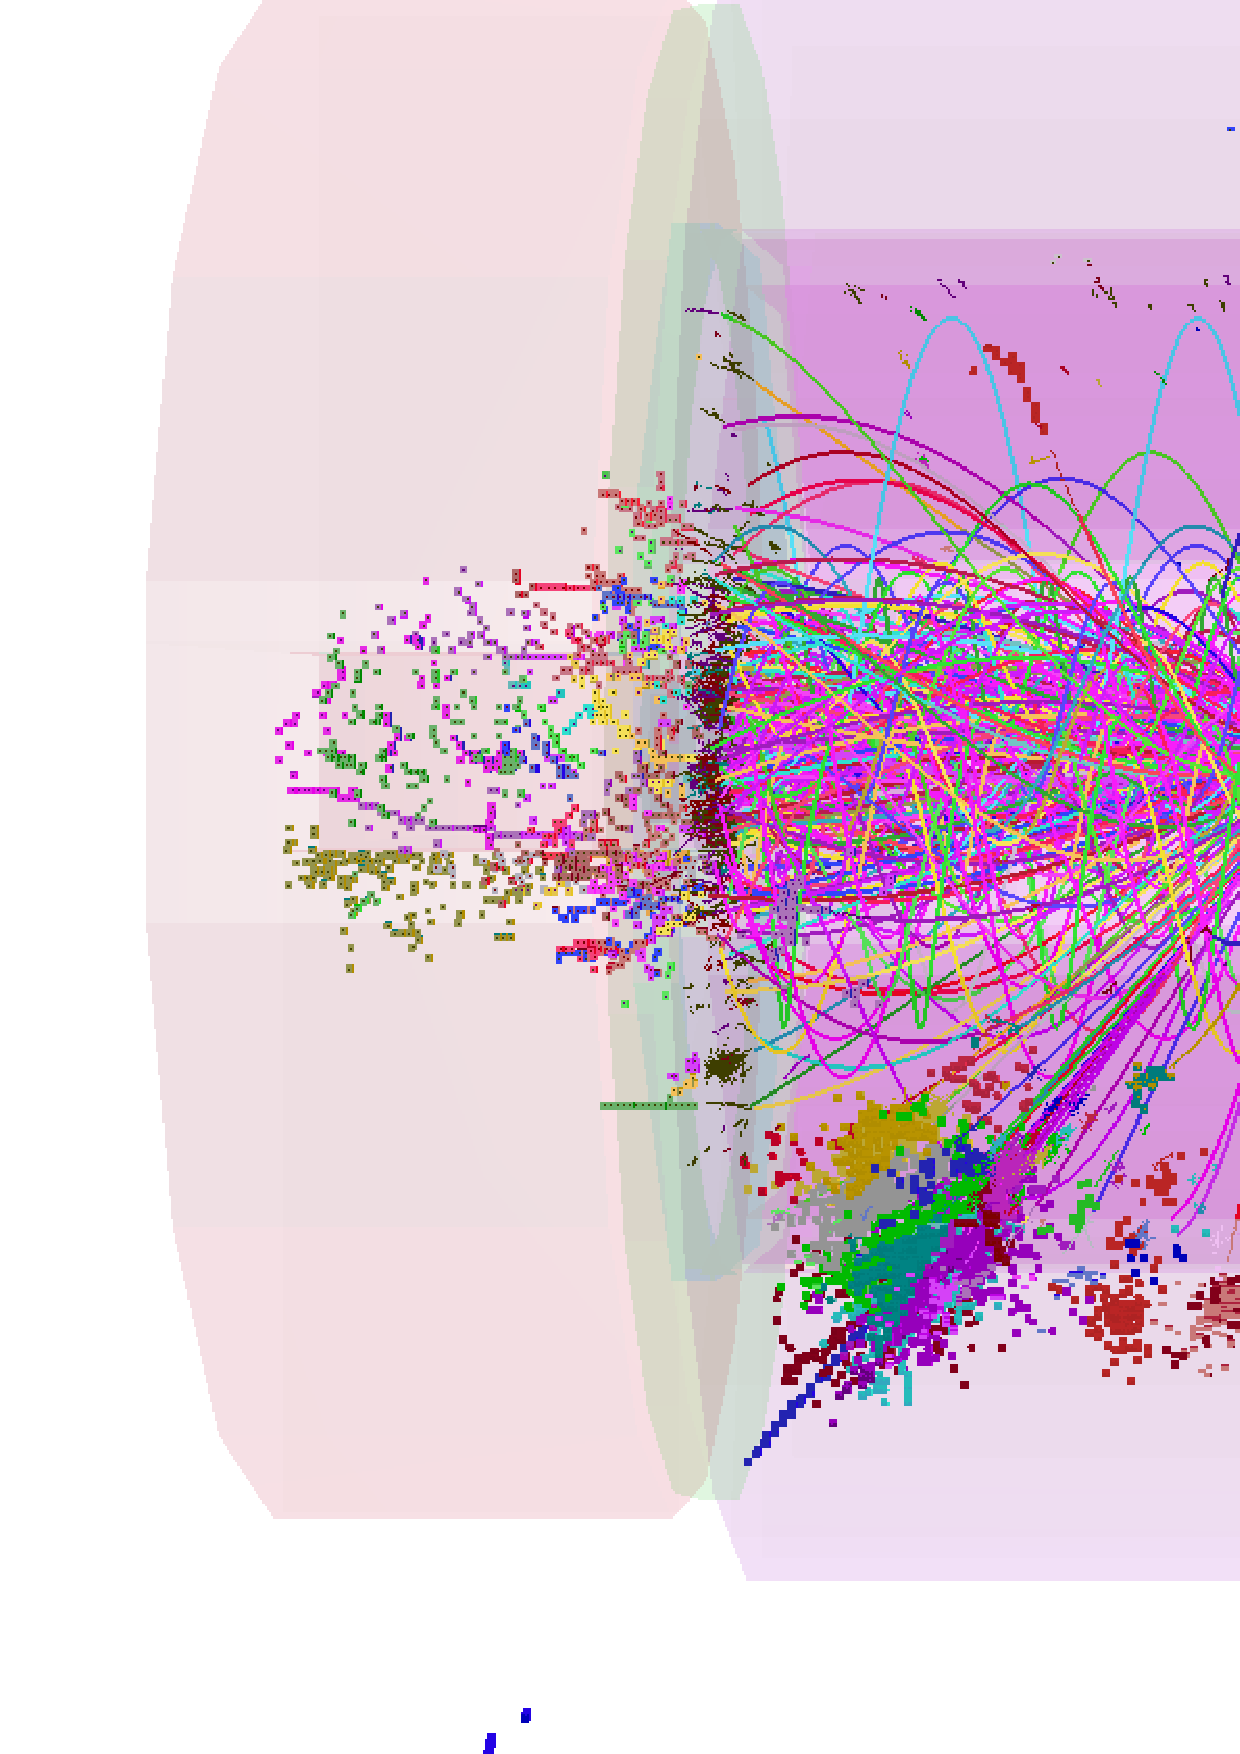
\includegraphics[width=\textwidth]{pandora/evtDisplayggHad1}
    \caption{}
    \label{fig:pandoraEvtDisplayggHad1}
  \end{subfigure}
  \begin{subfigure}[b]{0.45\textwidth}
    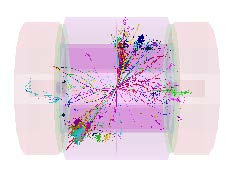
\includegraphics[width=\textwidth]{pandora/evtDisplayggHad2}
    \caption{}
    \label{fig:pandoraEvtDisplayggHad2}
  \end{subfigure}
\caption[Effect of the suppression of the background with the tight \PFO selection.]
{Reconstructed particles for a time window of 10\,ns (100 \,ns in \HCAL barrel) in a simulated \HepProcess{\Pep\Pem \to \PHiggs\PHiggs \to \Ptop\APbottom\Pbottom\APtop} event in the \CLICILD dectro, with 60 bunch crossings of \ggHad background overlaid in \Figure{fig:pandoraEvtDisplayggHad1}. The effect of applying tight \PFO section cuts is shown in \Figure{fig:pandoraEvtDisplayggHad2}.  The figures are taken from \cite{Marshall:2012ry}.}
\label{fig:pandoraEvtDisplayggHad}
\end{figure}

\subsection{\CLIC simulated particle masses}
\label{sec:pandoraCLICsimMass}

Another information used in the analysis (\Section{sec:doubleHiggsJetOptimisation}) with the \CLIC detector concept is the simulated mass and width of quarks and bosons. These values are listed in \Table{tab:pandoraCLICparticleMass} and are used for generating Standard Model samples.
\begin{table}[htbp]
\centering
\smallskip
\begin{tabular}{l r  r }
\hline
Particle &  Mass ($GeV/c^2$) & Width ($GeV/c^2$) \\
\hline
\Pup, \Pdown, \Pstrange quarks& 0 &  0\\
\Pcharm quark& 0.54 &  0\\
\Pbottom quark& 2.9 &  0\\
\Ptop quark& 174 & 1.37\\
\PW & 80.45 &  2.071\\
\PZ & 91.188 &  2.478\\
\hline
\hline
\end{tabular}
\caption[Masses of quarks and bosons used for  generating Standard Model samples.]%
{The masses and widths of quarks and bosons used for  generating Standard Model samples. The \PHiggs mass is specified for individual samples. The table is taken from \cite{Linssen:2012hp}.}
\label{tab:pandoraCLICparticleMass}
\end{table}



\section{Analysis software}

In the previous sections the automated reconstruction tools are described in detail. This section is dedicated to the common automated analysis software, which will be used in the analysis described in subsequent chapters.

\subsection{Monte Carlo truth linker}
\label{sec:pandoraMCtruthLink}
It is extremely useful to be able to associate reconstructed objects to the Monte Carlo (MC) simulated particles, to develop algorithms or to optimise event selection. The MC truth linker processor provides the link between a MC particle and a  reconstructed calorimeter hit. From the link, the main MC particle, contributing to a reconstructed \PFO or a group of \PFOs (jet), can be determined.

\subsection{Jet algorithms}
\label{sec:pandoraJetAlg}

For the linear collider, thanks to the high granular calorimeter and advance PFA software, the starting point for analysis are individual Particle Flow Objects (PFOs), as well as individual tracks. Each of the PFOs encodes four-momentum and position information. At the same time, tracks would have momentum and position information. However, sometimes it is useful to group PFOs and tracks into jets, which are the results of hadronisation processes from high energy particles like quarks or gulons.

A jet is typically a visually obvious structure in an event display. The momentum and the direction of a jet tend to resemble the original particle. Despite the relative simplicity of identifying jets visually, it is a challenge for a pattern recognition program to identify jets effectively and efficiently. Early work on jet finding started in 1977 \cite{Sterman:1977wj}, where later development can be found in reviews \cite{Moretti:1998qx,Salam:2009jx,Ali:2010tw}. This section is based on these reviews.

There are two large families of jet finding algorithm: cone based algorithms, and sequential combination algorithms. The cone based algorithms are briefly discussed in \Section{sec:pandoraConeCluster} in the context of the \pandora reconstruction. Here the focus is on the sequential combination algorithms.

Sequential combination algorithms typically calculate a pair-wise distance metric between a seed and a other particle. Pairs with the smallest metric are combined into a jet. The distance metric will be updated after a combination. This procedure is repeated until some stopping criterion are satisfied. The different jet algorithms typically differ in the distance metric and stopping criterion.
%, and a pair with smallest metric will be combined.

The chosen jet algorithm implementation for this thesis is the FastJet C++ software package \cite{Cacciari:2011ma,Cacciari:2005hq}, providing a wide range of jet finding algorithms. The implementation in the Marlin software package is called the MarlinFastJet. The symbols in the subsequent discussion follow the convention in \cite{Cacciari:2011ma}.

\subsubsection{\kt algorithm}

Longitudinally-invariant \kt algorithm \cite{Catani:1993hr,Ellis:1993tq} is one of the common sequential combination algorithms for \pp collider experiments. There are two variants: inclusive and exclusive. In the inclusive variant, the symmetrical pair-wise distance metric between particle $i$ and $j$, $d_{ij}$ or $d_{ji}$, and the beam distance, $d_{iB}$, are defined as
\begin{equation}
&d_{ij} = d_{ji} = \min\!\parenths{\pT_{i}^{2},\!\pT_{j}^{2}}\frac{\DeltaOf{R_{ij}^{2}}}{R^{2}}, \\
&d_{iB} = \pT_{i}^2,
\end{equation}
where $\pT_{i}$ is the transverse momentum of particle $i$ with respect to the beam ($z$) direction, and $\DeltaOf{R_{ij}^{2}}$ is the measurement of angular separation of particle $i$ and $j$, defined as $\DeltaOf{R_{ij}^{2}} = \parenths{y_i - y_j}^2 + \parenths{\phi_i - \phi_j}^2$, where $y_i = \frac{1}{2}\ln\!\frac{E_i + {p_z}_i}{E_i - {p_z}_i}$ and $\phi_i$ are particle $i$'s rapidity and azimuthal angle. $R$ is a free parameter controlling the jet radius.

If $d_{ij} < d_{iB}$, particle $i$ and $j$ are merged, with the \fourMomentum of particle $i$ updated as the sum of the two particles. Otherwise, particle $i$ is set to be a final jet, and deleted from the particle list. The above procedure is repeated until no particles are left.

The exclusive variant is similar to the inclusive variant. First difference is that when  $d_{iB} < d_{ij}$, particle $i$ is discarded and part of the beam jet. The beam jet contains particles that are considered from the beam induced background. The beam jet is not used as a output. The second difference is that when both $d_{ij}$ and $d_{iB}$ are above some threshold, $d_{cut}$, the clustering will stop. In practise, the exclusive mode allows a specified number of jets to be found, which will automatically choose the $d_{cut}$. The inclusive mode would find as many jets as the algorithm allows. An example usage of the exclusive \kt algorithm can be found in \Section{sec:doubleHiggsJetOptimisation}.

\subsubsection{Durham algorithm}
\label{sec:pandoraJetDurham}
The Durham algorithm \cite{Catani:1991hj}, also known as \ee \kt algorithm, is commonly used for the \ee collider experiments. It has a single distance metric:
\begin{equation}
d_{ij} = 2\min\!\parenths{E_i^2,\!E_j^2}\!\parenths{1 - \cosOf{\theta_{ij}}},
\end{equation}
where $E_i$ is the energy of particle $i$. $\theta_{ij}$ is the polar angle difference between particle $i$ and $j$. The Durham algorithm can only be run at exclusive mode, which means that the clustering will stop when $d_{ij}$ is above some threshold, $d_{cut}$.

Compared to the \kt algorithm, it uses energy instead of \pT in the distance metric, and it does not have a beam jet. This is because that for the \ee collider at low centre-of-mass energies, the beam induced background is not severe and the collisions energies are known.

\subsubsection{Jet algorithm for the \CLIC}

Although \CLIC is a \ee collider, the significant beam-induced background adds a large amount of energy. Therefore, traditional \ee jet algorithms, like the Durham algorithm, is not suitable for the \CLIC collision environment. Studies have shown that jet algorithms for the \pp colliders give better performances for the \CLIC \cite{Linssen:2012hp,LCD-Note-2010-006}.

%A more recent attempt at marrying merits from both the Durham and the \kt algorithms has resulted in the Valencia jet algorithm \cite{Boronat:2014hva}. It has shown promising improvement compared to the \kt algorithm.

%, which is used in the parallel  \eeToHHbbbb  sub-channel analysis in \Chapter{chap:DoubleHiggs} by collaborators.


%Why extra C++ implementation speed reduce O(n^3) to NlgN y, phi space, 2D KNN problem
\begin{comment}
\subsubsection{The \y{} parameter}
\label{sec:pandoraYparameter}
The \y{} parameter is calculated for each specific jet algorithm. It is a measure of the number of jets in an event. The \y{} parameter describes the transition of  the exclusive jet algorithm going from $N$ clustered jets to $N\!+\!1$ clustered jets. For example, $\y{23}$ would be the $d_{cut}$ value for a exclusive jet algorithm, above which the jet algorithm returns 2 jets, below which the jet algorithm returns 3 jets. Numerically the \y{} parameter is often much smaller than one. A typically way to convert the small number to a human acceptable range is to take the negative logarithm of the number.
\end{comment}
\begin{comment}
\subsection{The \lcfiplus}
\label{sec:pandoraLCFI}
Another useful analysis technique is to identify jets from \Pbottom and \Pcharm quarks. These jets have signatory topologies. A combination of vertex finding and multivariate analysis is used to identify \Pbottom and \Pcharm jets.

The flavour tagging processor, \lcfiplus \cite{Suehara:2015ura} is based on the LCFIVertex package \cite{Bailey:2009ui}, which was used in the simulation studies for the \ILCloi \cite{Abe:2010aa,Aihara:2009ad} and the \CLICcdr \cite{Linssen:2012hp}.  The current software is modular and can be used in any order. However here it will be described in the order used in a physics analysis.

%The current software is built for a future \ee collider.

The inputs are \PFOs. The vertex finding algorithms perform vertex fitting and identify primary and secondary vertices. There is a ``V0'' particle rejection step in which neutral particles decay into pairs of charged particles. The topology is similar to the decay of \Pbottom or \Pcharm hadrons. Hence it is important to remove the V0 particles to improve the heavy quark flavour tagging (see \Section{sec:pandoraPandoraTrack} for a similar V0 rejection).

Once the primary and secondary vertices are found, \PFOs are clustered in to jets. This jet clustering scheme ensures that the secondary vertices and the muons, identified from semi-leptonic decay, fall into the same jet. Therefore, it is consistent with  hadronic decay. The jet algorithms used are Durham and Durham modified algorithms(see \Section{sec:pandoraJetDurham}).

The next step is to refine vertices to improve the \Pbottom jet identification from the \Pcharm jet. Since the existence of two close by vertices is strongly correlated to a \Pbottom jet, the vertices refining step will reconstruct as many secondary vertices correctly as possible.

The last step is to gather the information about vertices and jets, and deploy a multivariate analysis. The multivariate classier used, Boosted Decision Tree,  is implemented in the TMVA software package \cite{Hocker:2007ht}. A series of flavour sensitive variables are calculated, and the classification is divided into four subset: jets with zero, one, or two properly reconstructed vertices, or a single-track pseudo-vertex. For each subset, a jet can either be classified to a \Pbottom jet, a \Pcharm jet, or a light flavour quark jet (\Pup, \Pdown or \Pstrange). The multiclass classifier's response is normalised across different subset, and they will be referred in the subsequent physics analysis as the tag value.

%The samples for training the multiclass classifier are \HepProcess{\Pep \Pem \to \PZ \APnu \Pnu} at \rootS{1.4}, where \PZ decays to \HepProcess{\Pbottom\APbottom}, \HepProcess{\Pcharm\APcharm}, or \HepProcess{\Pup\APup/\Pdown\APdown/\Pstrange\APstrange}.

The flavour tagging is performed after the initial jet reconstruction, and all the \PFOs in the reconstructed jets are input into the \lcfiplus flavour tagging processor. Therefore, the classifier in the \lcfiplus processor is trained for a specific \PFO collection and a specific jet reconstruction algorithm. The outputs of the processor for a jet are three values, corresponding to the likelihood of the jet being a \Pbottom jet, a \Pcharm jet, or a light flavour quark jet.

%In this analysis, the classifier is trained with the optimal jet reinstruction choice, discussed in \Section{sec:doubleHiggsJetOptimisation}.
 % The selection efficiency of b-jets and c-jets with training samples is shown in \Figure{fig:doubleHiggs1.4Btag}.
\end{comment}


%\subsection{Event shape variables}
%\label{sec:pandoraEvtShape}
% ATTN used in tau chapter
\begin{comment}
Event shape variables are some useful global variables to describe the shape of the event, for example whether it is back-to-back, or homogenous in the solid angle.

The classical event shape thrust\cite{PhysRevLett.39.1587}, is defined as
\begin{equation}
T = \max_{\hat{t}}\!\frac{\sum_{i}\absOf{\hat{t}\!\cdot\!\vec{p_{i}}}}{\sum_{i}\absOf{\vec{p_{i}}}}
\end{equation}
where $\vec{p_{i}}$ is the momentum vector of the particle $i$. Summation is over all particles in the event. Thrust axis, $\hat{t}$, is a unit vector. (Principle) Thrust value, $T$, is 1 for a perfect pencillike back-to-back two-jet event, and 0.5 for a perfect spherical event. The thrust value is useful in picking out back-to-back two-jet event. Thrust axis is useful to separate each jet in a back-to-back two-jet event.
\end{comment}
\begin{comment}
A related variable , sphericity is  derived from the sphericity tensor \cite{PhysRevLett.35.1609}. The sphericity tensor is  defined as
\begin{equation}
\bm{S^{\alpha\beta}} = \frac{\sum_{i}p^{\alpha}_{i}p^{\beta}_{i}}{\sum_{i}\absOf{\vec{p_{i}}}^2},
\end{equation}
where $\vec{p_{i}}$ is the momentum vector of the particle $i$. Summation is over all particles in the event. $\alpha$ and $\beta$ refer to the x, y, z coordinate axis. Eigenvalues of tensor $\bm{S}$ can be found, or in this case diagonalisation of the matrix $\bm{S}$, denoted with $\lambda_{1}$, $\lambda_{2}$, $\lambda_{3}$. The normalisation condition requires $\lambda_{1}\!\geqslant\! \lambda_{2} \! \geqslant \! \lambda_{3}$ and $ \lambda_{1} \! + \! \lambda_{2} \! + \! \lambda_{3} \! = \! 1 $. Sphericity, $S$, is defined in terms of $\lambda$,
\begin{equation}
\sphericity = \frac{3}{2}\parenths{\lambda_{1} \! + \! \lambda_{2}}.
\end{equation}
\sphericity, is 0 for a perfect pencil-like back-to-back two-jet event, and 1 for a perfect spherically symmetric event.

Aplanarity is another useful event shape variable that distinguishes spherical symmetrical events from planar and linear events. The definition is
\begin{equation}
S = \frac{3}{2}\parenths{\lambda_{1}},
\end{equation}
where $\lambda_{1}$ is the largest eigenvalue in the diagonalised sphericity tensor, $\bm{S^{\alpha\beta}}$.



\section{Miscellaneous}

An event in a collider experiment refers to one collision and the subsequent energy deposition in the detector. An event corresponds to a certain type of physics process.

Often we are dealing with extracting a type of events, from a large number of other events. The signal, or signal events refer to events of interests. Other events are referred to as the background, or background events.

Typical metrics of signal selection is efficiency and purity. This toy example illustrates definitions of efficiency and purity.

\begin{table}[!tbp]
\begin{tabular}{lrr}
\hline
\hline
Event Number  &  True Signal & True Background  \\
\hline
Selected Signal & $N_S$ & $N_1$ \\
Selected Background & $N_2$ & $N_B$ \\
\hline
\hline

\end{tabular}
\caption[A toy example to demonstrate definitions of efficiency and purity.]%
    {A toy example to demonstrate definitions of efficiency and purity.}
\label{tab:analysisToyExample}
\end{table}
Signal selection efficiency is defined as $\frac{N_S}{N_S \! + \! N_2}$. Signal selection purity is defined as $\frac{N_S}{N_S \! + \! N_1}$.
Significance is a quantity that is similar to purity, $\frac{N_S}{\rootOf{N_S \! + \! N_1}}$

When we are describing particles, light lepton, \llight, refer to electrons, \Pem, and muons, \Pmuon. Light quarks, \qlight, refer to up quark, \Pup, down quark, \Pdown, and strange quark, \Pstrange.
\end{comment}

\section{Multivariate Analysis}
\label{sec:pandoraMVA}

Multivariate analysis (MVA) has become increasingly common in high energy physics. MVA is typically used as the last step of the physics analysis to select signal from background. It can be viewed as an advanced tool for regression or classification. Compared to the traditional cut-based method, modern machine learning techniques offer much improvement to the data analysis. The implementation of the machine learning techniques used in this thesis are provided by  TMVA \cite{Hocker:2007ht}.

A typical machine learning MVA classification involves two classes, also known as signal and background. A machine learning model needs to be trained with training data. The model requires a set of discriminative variables, which separate the signal from background. The trained model will be applied onto the testing data for signal extraction. The response of the model could be a classification with two-class outcome of  signal or background.   The response  could also be a regression with output in a continuous spectrum.

%R, where the user decides the value to separate signal from background.

There should be three statistically independent samples for the MVA: one sample for the training; another sample for the validation, including optimisation and checking for overfitting; and the last sample for testing. However, due to technical reason (TMVA only natively supports two samples), sometimes the same sample is used for the validation and the testing, which is an acceptable usage with samples of large statistics.

This classification scheme can easily be extended to multiple classes, implemented in TMVA with the multiclass class. The multiclass class is used in the tau decay mode classification in \Section{sec:tauMVA} and in the flavour tagging classifier in \Section{sec:doubleHiggsFlavourTagging}.

\subsection{Optimisation and overfitting}
\label{sec:pandoraMVAoptimisation}

The optimisation of the model refers to selecting the optimal free parameters of the model. One could build a complex model which fits the training samples very well, but it would not be optimal for another testing sample. A simple model is less prone to statistical fluctuation of samples, however, it might be too simple to achieve the optimal modeling. The former case is known as overfitting, or overtraining. The latter case is called underfitting, or undertraining.

The compromise is clear. The optimal model is the one between overfitting and underfitting. In practice, this involves building the model with increasing complexity, and finding the point where overfitting occurs.


\FIGURE{fig:doubleHiggsMVAovertraining} shows a typical overfitting plot. Overfitting is defined when the efficiency of the signal selection in the training samples increases, but the efficiency in the testing sample decreases. The example in \Figure{fig:doubleHiggsMVAovertraining}  is chosen from the double Higgs analysis at \rootS{3}, using the Boosted Decision Tree model. The efficiency of the signal selection is defined as the signal fraction when the background fraction is 1\%, reported by the TMVA training process. In \Figure{fig:doubleHiggsMVAovertraining} , the depth of the tree, or the number of layers in the tree, reflects the complexity of the model. From tree depth two to fix, the efficiency for both testing and training samples increases. From tree depth six onwards, overfitting occurs. In this particular example, one should choose a tree depth fewer than seven to avoid overfitting.

\FIGURE{fig:doubleHiggsMVAovertraining}  can be repeated with a different split of training and testing samples to avoid the statistical fluctuation in samples. This allows for a better estimation of where overfitting occurs. However, this method is not used as the TMVA does not support such a method.

   %There are better methods
%There are methods to assign the error on the selection efficiency, as the training and testing efficiency would fluctuate wit . Thus one can make a better choice of parameters to avoid overfitting. These methods were not implemented due to the technical capacity provided by the TMVA.

\begin{figure}[!tbp]
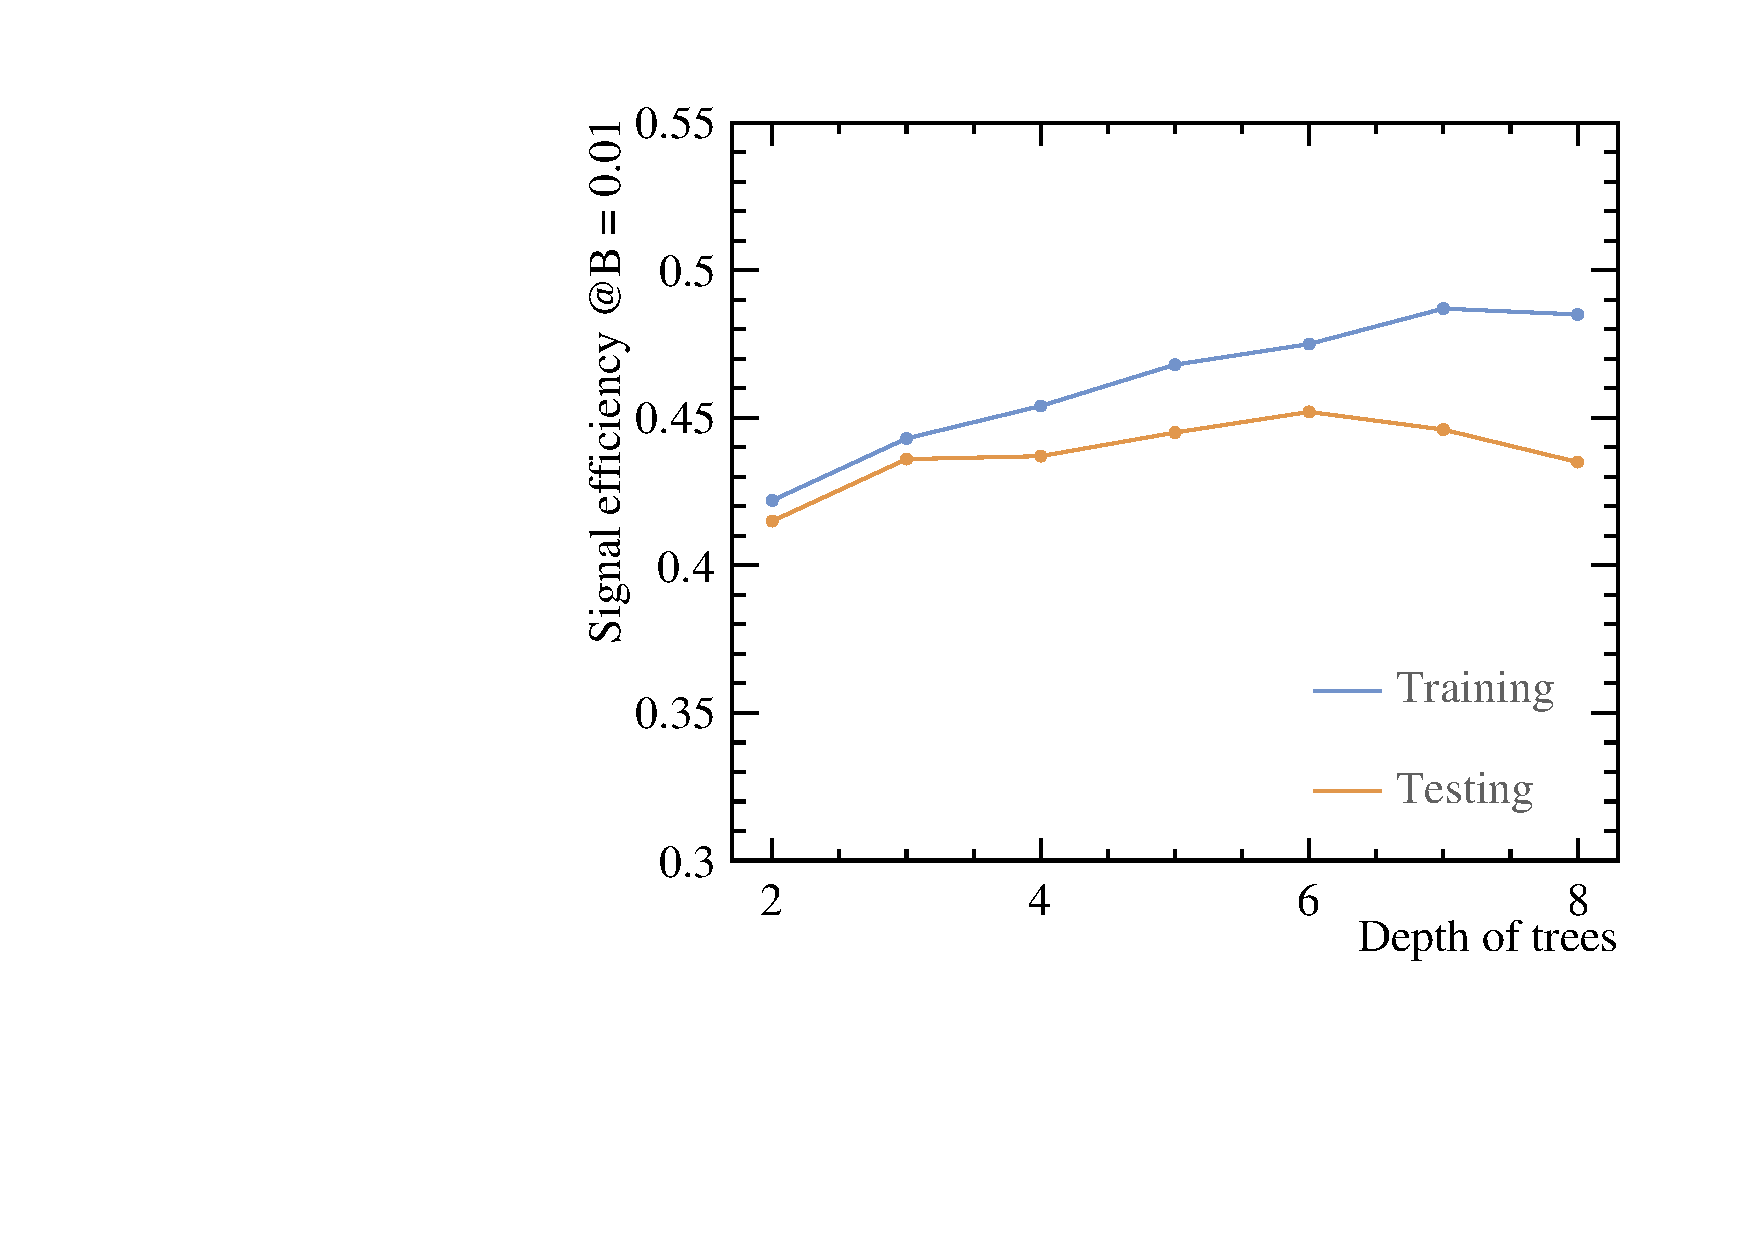
\includegraphics[width=0.45\textwidth]{doubleHiggs/DepthOfTrees.pdf}
\caption{Example of model efficiency as a complexity of the model parameters. Here the model is a boosted decision tree. The model parameter is the depth of tree. The y-axis is the signal efficiency when the background efficiency is 1\%. From tree depth six onwards, overfitting occurs.}
\label{fig:doubleHiggsMVAovertraining}
\end{figure}


\subsection{Choice of models}

The model can be as simple as a cut-based, a likelihood, or a linear regression model. The model can also be as complicated as non linear tree, non linear neutral network, or support vector machine. Regardless of the model complexity, the choice of the most optimal classifier is often data driven to match the nature of the sample. For example, a non-linear model is the best to model a non-linear response. The  comparison between different models without individual tuning is not rigourous.  Nevertheless, as researchers in the machine learning suggested, the boosted decision tree is probably the best out-of-the-box machine learning method. A neutral network model could potentially be better than the boosted decision tree model, but it requires more tuning, and it is less intuitive to interpret such a model. For these reasons, the boost decision tree model (BDT) is often the choice of machine learning model in high energy physics. And it is used in various physics analysis in this thesis. Before describing the BDT in detail, we will first visit some simpler models.

%the traditional rectangular cut model, and the Projective Likelihood method, which is used in the photon ID in the \pandora in \Section{}.

\subsubsection{Rectangular Cut model}

The rectangular cut method, probably the most intuitive model, optimise cuts to maximise some specific pre-defined metrics. The metric could be the signal efficiency for a particular background efficiency. Alternatively, the metric can be the significance, $\frac{S}{\rootOf{S\!+\!B}}$, where $S$ and $B$ are signal and background numbers, respectively.

Discriminative variables give better separation power when they are gaussian-like and statistically independent. Therefore it is common to decoorelate  the variables and gaussian transform them before using the rectangular cut MVA.

Because of its simplicity, the cut method is often performed manually, much more often at times pre-dating the spread of machine learning methods. It is still commonly used for the pre-selection step before the MVA (see \Section{sec:doubleHiggsPreSelection}), and other simple cases. Unless specified, the optimal rectangular cuts proposed in this thesis for various physics analyses are found manually.

\subsubsection{Projective Likelihood model}
\label{sec:pandoraLikelihood}

The projective likelihood model with probability density estimators (PDE) is used in \pandora for the photon ID,  due to its simplicity and low requirement on computing resources. The \pandora implementation is discussed  in \Section{sec:photonPDE}.
%Probability density estimators for each input variable combined in likelihood estimator (ignoring correlations

The likelihood classifier implemented in the TMVA calculates the probability density for each discriminative variable, for signal and background (hence PDE approach). The overall signal and background likelihood are defined as products of the individual probability density. The likelihood ratio, $R$, is then defined as the signal likelihood over signal plus background likelihood. TMVA implementation also fits an underlying function to the probability density.

%The \pandora implementation simply uses binned likelihood ratio, $R$, as the output, due to the simplicity. The sub-categories for the \pandora implementation are determined by the cluster energy.

Similarly to the rectangular cut method, the likelihood model works better with decorrelated, gaussian like variables.

%The \pandora implementation did not decorrelate nor transform the variables, to keep implementation fast.


\subsubsection{Decision tree model}
\label{sec:pandoraDecisionTree}
 %is a non linear tree based model

Before discussing Boost decision tree (BDT), it is necessary to introduce the decision tree model. The decision tree is a non linear tree based model. Its rather complex nature requires a careful explanation of many concepts.

The decision tree is a binary tree, where each node, the splitting point, uses a single discriminative variable to decide whether an event is signal-like (``goes down by a layer to the left''), or background-like (``goes down by a layer to the right''). At each node, samples are divided into signal-like and background-like sub-samples. The tree growing starts at the root node, and stops at certain criterion, which could be the minimum number of events in a node, the number of layers of the tree, or a minimum/maximum signal purity.

The training of the decision tree is to determine the optimal cut at the node by minimising the metric. The probability of the cut producing the signal is $p$. Three commonly used metrics for two-class classification are
\begin{enumerate}
\item Misclassification error:  $1 - \max\parenths{p\!,\!1\!-\!p}$,
\item Gini index: $2p\parenths{1\!-\!p}$,
\item Cross-Entropy or deviance: $-p\log{p}-\parenths{1\!-\!p}\log\parenths{1\!-\!p}$.
\end{enumerate}

The applying of a trained decision tree is to transverse along the tree. The event is classified as signal or background, depending on whether it falls in the signal-like or background-like end node.

\begin{figure}[!tbp]
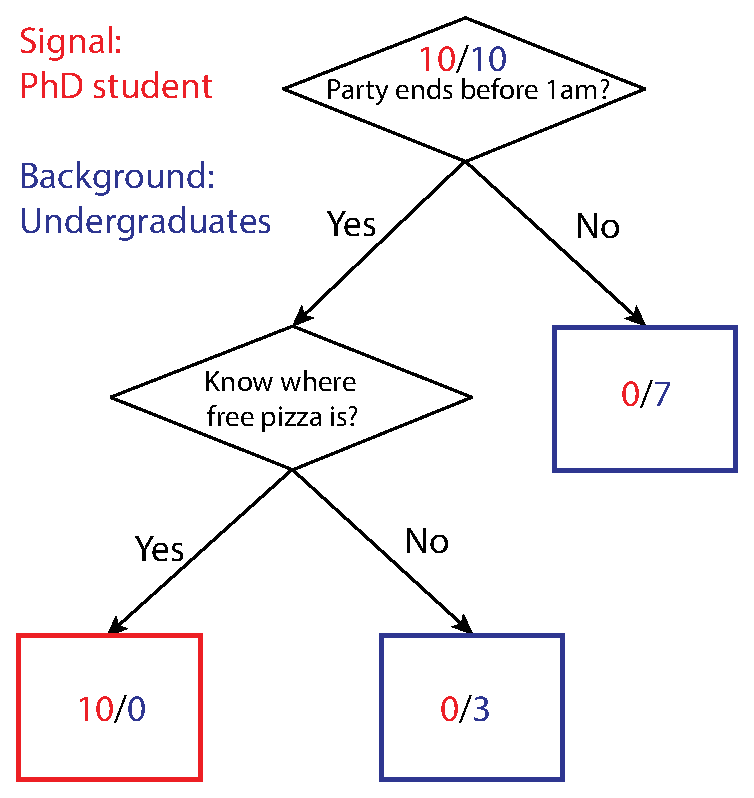
\includegraphics[width=0.45\textwidth]{doubleHiggs/mva/BDTcomic}
\caption[Example of a decision tree. ]
{Example of a decision tree. Numbers in each node represent number of PhD student (red) and number of undergraduate student (blue) after each cut.}
   \label{fig:doubleHiggsMVAdecisionTree}
\end{figure}

\FIGURE{fig:doubleHiggsMVAdecisionTree} illustrate a simple example of a decision tree. The signal class is the PhD student and the background class is the undergraduate student. The depth of this imbalance binary  tree is 2. A node is represented by a diamond.  The signal-like node is the red rectangle and the background-like nodes are blue rectangles. The tree is constructed with two possible cuts, ``Party ends before 1am'' and ``Know where free pizza is''. The attribute of samples is listed in \Table{tab:doubleHiggsDecisionTreeComic} and  \Table{tab:doubleHiggsDecisionTreeComic2}. To demonstrate the choice of the first layer cut, the Gini index metric is used. If the first cut is ``Party ends before 1am'', the probability of the cut producing the signal, $p$, is $\frac{10}{13}$. Gini index is $2p\parenths{1\!-\!p} \backsimeq 0.36 $. If the first cut is ``Know where free pizza is'', $p=\frac{10}{15}$. Gini index is $2p\parenths{1\!-\!p} \backsimeq 0.44 $. Therefore, the first cut is ``Party ends before 1am''.

The simple tree in \Figure{fig:doubleHiggsMVAdecisionTree} is grown fully as each end node contains signal or background only. To use the trained decision tree, if there is s student who ends the party before 1am and knows where a free pizza is located, then the student is classified as a PhD student.

\begin{table}[!tbp]\centering

\begin{tabular}{lrr}
\hline \hline
PhD student & Party ends before 1am  & Party ends after 1am\\
\hline
Know where free pizza is & 10 & 0 \\
Not know where free pizza is & 0 & 0 \\
\hline \hline
\end{tabular}
\caption
{The attribute of the PhD student class for the decision tree example shown in \Figure{fig:doubleHiggsMVAdecisionTree}.}
\label{tab:doubleHiggsDecisionTreeComic}
\end{table}
\begin{table}[!tbp]\centering

\begin{tabular}{lrr}
\hline \hline
Undergraduates & Party ends before 1am  & Party ends after 1am\\
\hline
Know where free pizza is & 0 & 5 \\
Not know where free pizza is & 3 & 2 \\
\hline \hline
\end{tabular}
\caption
{The attribute of  the undergraduates class for the decision tree example shown in \Figure{fig:doubleHiggsMVAdecisionTree}.}
\label{tab:doubleHiggsDecisionTreeComic2}
\end{table}


\paragraph{To improve decision tree}

The decision tree has a low bias, but high variance. This means it is very easy to construct a tree, which is also the best tree, that fits the training data very well, but the tree would not be optimal for the testing sample. To overcome the instability of the decision tree, many methods have been developed. The most successful one is boosting and bagging.

Boosting: it is a technique where the misclassified events receives a higher weight than the correctly classified events. Therefore, when the training is iterated, the misclassified events would receive higher and higher weights and be more likely to be classified correctly. The boosting is done at every iteration, which can be a few hundred or a few thousand times. This will create a ``forest'' of many trees. The final output could be a majority vote, by transversing the event to the end node for each tree in the forest.

Bagging: also known as boot-strap, it is a method that select a simple random sub-sets of the training sample, and apply the model. In this case, every boosting iteration takes a bagged sample, rather than the whole sample.

Random Forest: when a tree is grown, a randomly selected sub-set of all variables are used to grow the tree. This method is know to reduce the variance of the tree.

\subsubsection{Boosted decision tree model}
\label{sec:analysisBDT}

Boosted decision tree (BDT) contains a forest of decision trees , where each tree is iterated many times using a technique called boosting.   By overcoming the instability of a single  decision tree, BDT is often regarded as  the best out-of-the-box machine learning method. There are two common boosting methods: adaptive boosting and gradient boosting. First introduced in \cite{FREUND1997119}, the adaptive boosting is discussed in further details, as it is simpler to understand than gradient boosting.

The basic idea of adaptive boosting is that the tree making procedure focuses on events which are difficult to classify correctly. By assigning a weight to each event,   after each tree making iteration, the weights for misclassified events are gradually increased. Therefore misclassified events get more attention.

A simple example is provided. Assuming that the tree classifier output is denoted as  -1 or 1. One can think of -1 as background and 1 as signal. Suppose there are $N$ events and $M$ iterations (trees). $B$ represents if a event is misclassified. For the $i^{th}$ event in the  $m^{th}$ tree,  $B_{i,m} = 1$ if the event is misclassified and 0 if the event is correctly classified.

The adaptive boosting algorithm, adapted from \cite{hastie2009elements},  is outlined below.

\begin{itemize}
  \item At the initialisation stage,  event weight is initialised to $w = 1 / N$ for every event, for $N$ total events.
  \item Iterate $M$ times. M is the total number of trees. For iteration $m$:
    \begin{itemize}
      \item Create a $m^{th}$ tree  with weighted samples.
      \item Update $m^{th}$ tree error function, $err_m = \frac{\sum_{i = 1}^{N} w_{i,m-1} B_{i,m} }{\sum_{i = 1}^{N}w_{i,m-1}}$.
      %, where $B_{i,m} = 1$ if $i^{th}$ event is misclassified, 0 if $i^{th}$ event is correctly classified. $w_{i,m-1}$ is the event weight for $i^th$ event generated in previous iteration.
      \item Update $m^{th}$ tree weight,  $\alpha_m = \log\parenths{\frac{1 - err_m}{err_m}}$
      \item Update $i^{th}$ event weight, $w_{i,m} = w_{i,m-1} e^{\alpha_m B_{i,m} }$.
    \end{itemize}
  \item The output, $G(x)$, for testing event $x$ is a weighted vote from all M trees:
  \begin{equation}
    G(x)=
     \begin{cases}
      -1, & \mbox{if} \sum_{m=1}^{M}\alpha_mG_m(x) < 0 , \\
      1, & \mbox{otherwise}.
    \end{cases}
  \end{equation}
\end{itemize}

In each iteration, if the $i^{th}$ event is misclassified, the weight increases by a factor of $(1 - err_m)/(err_m)$. Otherwise, the event weight does not change.

The power of the adaptive boosting  is to dramatically improve the performance of a weak classifier. A weak classifier is a classifier which is sightly better than random guessing. A small decision tree would be a weak classifier. By sequentially applying many weak classifier with weighted samples, the final ``forest'' is very robust with very good performance.

%A weak classifier is one whose error rate is only slightly better than random guessing. The purpose of boosting is to sequentially apply the weak classification algorithm to repeatedly modified versions of the data,

TMVA implementation of the BDT for the output is using a likelihood estimator, depending on how often an event is classified as signal in the forest. The likelihood number is later used to select signal from background.

\paragraph{Optimisation of Boosted Decision Tree}
\label{sec:pandoraMVAbdtVar}
Many parameters of the BDT can be optimised, described below.

The most important parameter is the depth of a tree, which determines how many end nodes the tree has, or the degrees of freedom of the tree. The related parameter is the number of trees. Experience shows that using many small trees yields the best result. The performance as a function of the depth is shown in \Figure{fig:doubleHiggsMVAovertraining}.

The number of trees is another important parameter. Intuitively large number of trees leads to overfitting. However, it has been shown that a large number does not lead to overfitting. Therefore there is a debate on the metric to determine the optimal number of trees.

The minimum number of events in a node, which is a stopping criteria for tree growing, affects the size of the tree. But it is less influential than the depth of the tree.

The boosting has two variants in TMVA implementation: adaptive boost and gradient boost.

The learning rate of the adaptive boost  controls how fast the weight changes for events in each boosting iteration. Experience shows that a small learning rate with many trees works better than a large learning rate with fewer trees.

The shrinkage rate in the gradient boost is similar to the learning rate in the adaptive boost. The shrinkage rate controls how fast the weight changes for events in each boosting iteration. Again a small value is preferable.

The usual choice of the metric for the optimal cuts is either the Gini index or the cross-entropy. Typically the Gini index metric is chosen. It makes little difference to performances, comparing to the cross-entropy metric.

The number of bins per variable is necessary to make tree growing efficient. Discrete binned variables are faster to computer than continuous variables. The parameter does not impact the performance much. However, variables should be pre-processed before going into the model. For example, the variable should be limited to a sensible range to avoid the extremes. The variable should also be transformed to obtain a more uniform distribution, if the original distribution is highly skewed.

For the end node, it is determined as either signal-like or background-like, based on the majority of the training events in the end node. Numerically, it corresponds to 1/0. However, the end node could also use signal purity as the output, resulting in a continues spectrum of [0,1]. The adaptive boosting algorithm is modified for the output value continuous spectrum.

The bagging fraction determines the fraction of randomly selected samples used in each boosting iteration. By choosing a smaller value, samples between each boosting iteration are less correlated. Hence the overall performance improves.

The DoPreSelection flag allows the classifier to throw away phase spaces where there are only background events.

\subsection{Multiple classes}
\label{sec:pandoraMVAmulticlass}
% ATTN used in tau chapter

The above discussion is done assuming two classes - signal and background. The argument can be extended to multiple classes. There are two ways for the training. ``One v.s. one'' means that each class is trained against each other class, and the overall likelihood is normalised. The second way to train is called ``one v.s. all'', when each class is trained against all other classes.

Using a three-class example, A, B and C, ``one v.s. one" scheme trains A against B, B against C, and C against A. Then the likelihood is normalised. ``One v.s. all" would train A against B plus C, B against A plus C, and C against A plus B.

TMVA multiclass implementation uses the ``one v.s. all" scheme. For each class, the multiclass classifier will train the class as the signal against all other final states as the background. This process is repeated for each class. The classifier output for a single event is a normalised response using all trained classifier, where the sum is one. The response of each class in a event can be treated as the likelihood. In the classicisation stage, the event is classified into a particular class if that class has the highest classifier output response.

The advantage of using the multiclass is that the correlation between different classes are accounted for. The classifier outputs are correctly adjusted for multiple classes. Hence one event can only be classified into one final state. The issue with the multiclass is that discriminative variables for all classes need enter the training stage, resulting in a large number of variables.

%TMVA multiclass implementation uses "one v.s. all" scheme. Multiclass is used in flavour tagging of jets, \Section{sec:pandoraLCFI}, and in the tau lepton final state separation study, \Section{}.

%Computational intensive jobs are processed either on the Cambridge High Energy Physics grid, or the \CLIC computing grid.
%Thanks computing resources. i.e. ILC VO, CLIC grid, etc. 
  %\chapter{Analysis technique}
\label{chap:Reconstruction}

\chapterquote{In preparing for battle I have always found that plans are useless, but planning is indispensable.}%
{Dwight D. Eisenhower}%:

Automated analysis is the only way to deal with the vast amount of data generated in the high energy physics. In the last chapter we described the automated reconstruction tools in details. This chapter is dedicated to the common automated analysis tools and techniques, which will be used in the analysis described in subsequent chapters.

For the linear collider, thanks to the high granular calorimeter, the starting point for analysis would be individual Particle Flow Objects, as well as individual tracks. Each of the PFOs encodes four-momentum and position information. For tracks, they would have momentum and position information.

However, sometimes it is interesting to group PFOs and tracks into jets, where a jet is the result of hadronisation process from high energy particles like quarks or gulons.

\section{Jet algorithm}

A jet is typically a visually obvious structure in a event display. The momentum and the direction of a jet tend to resemble the originated particle. Despite the relative easiness of identifying jets visually, it presents a challenge for a pattern recognition program to identify jets effectively and efficiently.

Early work on jet finding started in 1977 \cite{PhysRevLett.39.1436}, where later development can be found in reviews \cite{Moretti:1998qx,Salam:2009jx,Ali:2010tw}.

There are two large families of jet finding algorithm, cone based algorithm, and sequential combination algorithm. Cone based algorithm is briefly discussed in \Section{sec:pandoraConeClustering}.

Sequential combination algorithm typically calculate a pair-wise distance metric. Pairs with the smallest metric will be combined. The metric will be calculated and updated, and a pair with smallest metric will be combined. This procedure will be repeated until some stopping criterion are satisfied.

The chosen jet algorithm implementation is FastJet C++ software package \cite{Cacciari:2011ma,Cacciari:2005hq}, providing a wide range of jet finding algorithms. The implementation in Marlin software package is called MarlinFastJet. The symbols in the subsequent discussion about specific jet algorithms will follow \cite{Cacciari:2011ma}

\subsection{\kt algorithm}

One of the common sequential combination algorithms for \pp collider experiment, is longitudinally-invariant \kt algorithm \cite{Catani:1993hr,Ellis:1993tq}. In the inclusive variant, The symmetrical pair-wise distance metric between particle $i$ and $j$, and the beam distance, are defined as
\begin{equation}
&d_{ij} = d_{ji} = \min\!\parenths{\pT_{i}^{2},\!\pT_{j}^{2}}\frac{\DeltaOf{R_{ij}^{2}}}{R^{2}}, \\
&d_{iB} = \pT_{i}^2,
\end{equation}
where $\pT_{i}$ is the transverse momentum of particle $i$ with respect to the beam ($z$) direction, and $\DeltaOf{R_{ij}^{2}}$ is the measurement of angular separation of particle $i$ and $j$. Formally $\DeltaOf{R_{ij}^{2}} = \parenths{y_i - y_j}^2 + \parenths{\phi_i - \phi_j}^2$, where $y_i = \frac{1}{2}\ln\!\frac{E_i + {p_z}_i}{E_i - {p_z}_i}$ and $\phi_i$ are particle $i$'s rapidity and azimuthal angle. R is a free parameter controlling the jet radius.

If $d_{ij} < d_{iB}$, particle $i$ and $j$ are merged, with the \fourMomentum of particle $i$ updated as the sum. Otherwise, particle $i$ is set to be a final jet, and delete from the particle list. The above procedure is repeated until no particle left.

The exclusive variant is similar. First difference is that when  $d_{iB} < d_{ij}$, the particle $i$ is discarded and part of the beam jet. The second difference is that when both $d_{ij}$ and $d_{iB}$ are above some threshold, $d_{cut}$, the clustering will stop. In practise, exclusive mode allows a specified number of jets to be found, which will automatically choose the $d_{cut}$. The inclusive mode would fine as many jets as the algorithm allows.

\subsection{Durham algorithm}

Durham algorithm \cite{Catani:1991hj}, also known as \ee \kt algorithm, is commonly used \ee collider experiment. It has a single distance metric:
\begin{equation}
d_{ij} = 2\min\!\parenths{E_i^2,\!E_j^2}\!\parenths{1 - \cosOf{\theta_{ij}}},
\end{equation}
where $E_i$ is the energy of particle $i$. $\theta_{ij}$ is the polar angle difference between particle $i$ and $j$. Durham algorithm can only be run at exclusive mode, which means that the clustering will stop when $d_{ij}$ is above some threshold, $d_{cut}$.

Comparing to \kt algorithm, it uses energy instead of \pT in the distance metric, and it did not have a beam jet. This is because that for the \ee collider in the past, the beam induced background was not severe and collisions energy is known, \sqrtS.

\subsection{Jet algorithm for \CLIC}

Although \CLIC is a \ee collider, the significant beam-induced background adds a large amount of energy from \ggHad process. Therefore, traditional \ee jet algorithms, like Durham algorithm, is not suitable for \CLIC environment. Studies has shown that jet algorithms for \pp collider have better performance \cite{Linssen:2012hp,LCD-Note-2010-006}.

A more recent attempt at marrying merits from both Durham and \kt algorithms has resulted in Valencia jet algorithm \cite{Boronat:2014hva}. It had shown promising improvement comparing to \kt algorithm.

\begin{comment}
Why extra C++ implementation
speed reduce O(n^3) to NlgN
y, phi space, 2D KNN problem
\end{comment}

\subsection{\y{} parameter}
\y{} parameter is a commonly used quantity to describe the transition of exclusive jet algorithm going from $N$ clustered jets to $N\!+\!1$ clustered jets. For example, $\y{23}$ would be the $d_{cut}$ value for a exclusive jet algorithm, above which the jet algorithm returns 2 jets, below which the jet algorithm returns 3 jets.

Numerically \y{} parameter is often much smaller than one. A typically way to convert the small number to a human acceptable range is to take the minus logarithm of the number.

\section{Flavour tagging}
\label{sec:theoryFalvourTagging}

The latest software package for jet flavour tagging is \lcfiplus \cite{Suehara:2015ura}. It is based on the LCFIVertex package, which was used in the simulation studies for \ILCloi \cite{Abe:2010aa,Aihara:2009ad} and \CLICcdr \cite{Linssen:2012hp}. Current software is built in mind of a future \ee collider. Although the software is modular, it will be described in order that it will be used in a physics analysis,

The vertex finding algorithms perform vertex fitting and identify primary and secondary vertex. There is a ``V0'' particle rejection, which is when neutral particles decay or convert into a pair of charged tracks. The topology is similar to the decay of \Pbottom or \Pcharm hadrons. Hence it is important to remove the V0 particles to improve the heavy quark falvour tagging.

Jet clustering ensures that the secondary vertices and the muons identified from semileptonic decay are combined. Therefore, it is consistent with the hadronic decay. Jet algorithms used are Durham and Durham modified algorithms.

Vertices are refined to improve the \Pbottom jet identification from c jet. Two vertices is strongly correlated to a \Pbottom jet. Hence the vertices refining will reconstruct as many secondary vertices correctly as possible.

The final flavour tagging of the jet is done using multivariate analysis, which will be discussed in \Section{sec:theoryMVA}. Using TMVA software package \cite{Hocker:2007ht}, Boosted Decision Tree classier is used. A series of flavour sensitive variables are calculated, and the classification is divided four sub-set: jet with zero, one, or two properly reconstructed vertices, or a single-track pseudovertex. For each sub-set, a jet can either be a \Pbottom jet, a \Pcharm jet, or a light flavour quark jet (\Pup, \Pdown or \Pstrange). The multiclass classifier's response is normalised across different sub-set, and they will be referred in the subsequent physics analysis as the tag value.

\section{Multivariate analysis}
\label{sec:theoryMVA}

Multivariate analysis (MVA) has become increasingly common in high energy physics. MVA can be viewed as an advanced tool for regression or classification. Comparing to the traditional cut based method, modern machine learning technique offers much improvement in data analysis.

Software package for MVA used throughout this document is TMVA \cite{Hocker:2007ht}.

A typical machine learning MVA classification involves two classes, also known as signal and background. A machine learning model, called classifier in TMVA, needs to be trained with training data. The model requires a set of discriminative variables, which should separate signal from background. The trained model will be applied onto the testing data, for signal extraction. Response of the model could be signal/background, or be  a number in a continuous spectrum, where the user decides the value to separate signal from background.

Strictly, there should be three statistically independent samples for the MVA. One sample is for the training. Another sample for the validation, including optimisation and checking for overfitting. The last sample is for testing. However, due to technical reason, sometimes the same sample is used for the validation and the testing.

This classification scheme can be easily extended to multiple classes, implemented in TMVA with multiclass class.

\subsection{Optimisation and overfitting}

The optimisation of the model is to select the optimal free parameters of the model. One could build a complex model which fits the training samples very well, but it would not be optimal for another testing sample. A simple model is less prone to statistical fluctuation of samples, however, it might be too simple to achieve the optimal modeling. The former case is known as overfitting, or overtraining. The latter case is called underfitting, or undertraining.

The compromise is clear. The optimal model is one between overfitting and underfitting. In practice, this involves building the model with increasing complexity, and finding the point where overfitting occurs.

\begin{figure}[!tbp]
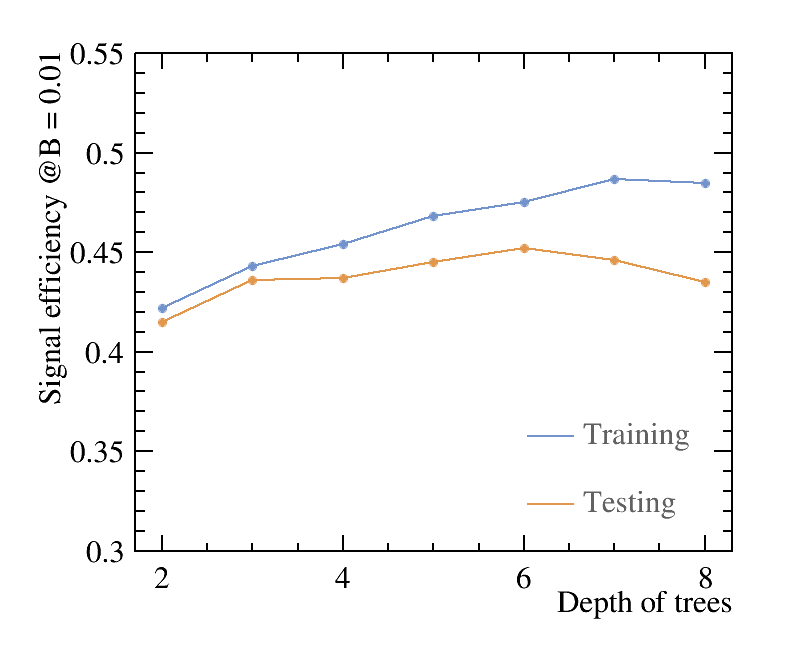
\includegraphics[width=\largefigwidth]{doubleHiggs/DepthOfTrees}
\caption[MVA overtraining]%
   {MVA overtraining}
   \label{fig:analysisMVAovertraining}
\end{figure}

\Figure{fig:analysisMVAovertraining} shows a typical overfitting plot. Overfitting is defined when the efficiency of signal selection in the training samples increases, but the efficiency in the testing sample decrease. Here the example is chosen from double Higgs analysis, using Boosted Decision Tree model, for \rootS{3} samples. The efficiency of signal selection is defined as the signal efficiency when background efficiency is 1\%, report by the TMVA training process. In the plot, the depth of the tree, or the number of layers in the tree, reflects the complexity of the model. From tree depth 2 to 5, the efficiency for both testing and training samples increases. From tree depth 6 onwards, the overfitting occurs. In this particular example, one should choose a tree depth fewer than 7 to avoid overfitting.

There are methods to assign the error on the selection efficiency. Thus one can make a better choice of parameters to avoid overfitting. These methods were not implemented due to the technical capacity provided by the TMVA.

\subsection{Choice of models}

The model, known as the classifier in TMVA, can be as simple as cut based, likelihood or linear regression. It can be complicated as non linear tree, non linear neutral network or support vector machine. Regardless of model complexity, the choice of most optimal classifier is often data driven. Also, given the free parameters in each model, the comparison between different models without individual tuning is not rigorous. Nevertheless, as researchers in the machine learning suggested, the boosted decision tree is probably the best out-of-the-box machine learning method. Neutral network could potentially be better than the boosted decision, but it requires more tuning, and it is less intuitive to interpret the model. For these reasons, boost decision tree (BDT) is often the choice of machine learning model in the high energy physics. And it is used in various physics analysis in this document.

Before describing BDT in detail, we will first visit the traditional rectangular cut model, and the Projective Likelihood method, which is used in the photon ID in the \pandora.



\subsection{Rectangular Cut}

Probably the most intuitive model, the rectangular cut method optimise cuts to maximise some specific metric. The metric could be the signal efficiency for a particular background efficiency. Alternatively, the metric can be the significance, $\frac{S}{\rootOf{S\!+\!B}}$, where $S$ and $B$ are signal and background numbers, respectively.

Discriminative variables gives better separation power when they are gaussian-like and statistically independent. Therefore it is common to decoorelate  the variables and gaussian transform them before using the rectangular cut MVA.

Because its simplicity, the cut method is often performed manual, much more often in the time pre-date the wide spread of machine learning methods. It is still commonly used for the pre-selection step before the MVA, and other simple usages. Unless specified, the optimal cuts proposed in this document for various physics analysis are found using the rectangular cut method manually.

\subsection{Projective Likelihood}

Projective likelihood model (PDE) is used in \pandora for the photon ID due to its simplicity and low requirement on computing resources.

PDE implemented in the TMVA calculates the probability density for each discriminative variable, for signal and background. The overall signal and background likelihood are defined as products of the individual probability density. The likelihood ratio, $R$, is then defined as the signal likelihood over signal plus background likelihood.

TMVA implementation also fits an underlying function to the probability density. The \pandora implementation simply uses binned likelihood ratio, $R$, as the output, due to the simplicity. The sub-categories for the \pandora implementation are determined by the cluster energy.

Similarly to the rectangular cut method, PDE works better with decorrelated, gaussian like variables. The \pandora implementation did not decorrelate nor transform the variables, to keep implementation fast.


\subsection{Boosted decision tree}
\label{sec:analysisBDT}
Boost decision tree (BDT) is a non linear tree based model. Its rather complex nature requires a careful explanation of many concepts within the BDT.

Decision tree is a binary tree, where each node, the splitting point, uses a single discriminative variable to decide whether a event is signal-like (``goes down by a layer to the left''), or background-like (``goes down by a layer to the right''). At each node, samples are divided into signal-like and background-like sub-samples. The tree growing starts at the root node, and stops at certain criterion, which could be the minimum number of events in a node, the number of layers of the tree, or a minimum/maximum signal purity.

The training of the decision tree is to determine the optimal cut at the node. The the probability of the cut produces the signal is $p$. Three commonly used metrics for two-class classification are
\begin{enumerate}
\item Misclassification error:  $1 - \max\parenths{p\!,\!1\!-\!p}$,
\item Gini index: $2p\parenths{1\!-\!p}$,
\item Cross-Entropy or deviance: $-p\log{p}-\parenths{1\!-\!p}\log\parenths{1\!-\!p}$.
\end{enumerate}

The using of a trained decision tree is to transverse along the tree. The event is classified as signal or background depending on whether it falls in the signal-like or background-like end node.

Decision tree has a low bias, but high variance. This means it is very easy to construct a tree that fits the training data very well, but the tree would not be optimal for the testing sample. To overcome the instability of the decision tree, many methods have been developed. The most successful one is boosting.

Boosting: it is a technique where the misclassified events receives a higher weight than the correctly classified events. Therefore, when the training is iterated, the misclassified events would receive higher and higher wights and more likely to classify correctly. The boosting is done at every iteration, which can be few hundred or few thousand time. This will create a ``forest'' of many trees. The final output could be a majority vote, by transversing the event to the end node for each tree in the forest.

Bagging: also known as boot-strap, it is a method that select a simple random sub-set of the training sample, and apply the model. In this case, every boosting iteration takes a bagged sample, rather than the whole sample.

TMVA implementation of the BDT for the output is using a likelihood estimator, depending on how often a event is classified as signal in the forest. The likelihood number is later used to select signal from background.

\subsection{Optimisation of Boosted decision tree}

Many parameters can be tuned. Hence we dedicate a small section to describe the tuning parameters.

The most important parameter is the depth of a tree, which determines how many end nodes a tree has, or the degrees of freedom of a tree. The related parameter is the number of trees. Experience shows that using many small trees yields the best result.

The minimum number of events in a node, which is a stopping criteria for tree growing, affects the size of the tree. But it is less influential than the depth of the tree.

The learning rate, which controls how fast the weight changes for events in each boosting iteration. Experience shows small learning rate with many trees work better than large learning rate with few trees.

The usual choice of the metric for the optimal cuts is either Gini index or cross-entropy. (See \Section{sec:analysisBDT}) We chose Gini index for out BDT usages, as it makes little difference to performances, comparing to the cross-entropy metric.

Number of bins per variables for the cut is necessary to make tree growing efficient. Discrete binned variables are faster to computer than continuous variables. The parameter does not impact the performance much. However, variables should be pre-processed before going into the model. For example, the variable should be limited to a sensible range to avoid the extremes. The variable should also be transformed to obtain a more uniform distribution, if the original distribution is highly skewed.

The boosting has two variant, adaptive boost and gradient boost. For all the BDT used in this document, adaptive boost is used.

For the end node, it is determined as either signal-like or background-like, based on the majority for the training event in the end node. Numerically, it corresponds to 1/0. However, the end node could also use signal purity as the output, resulting in a continues spectrum of [0,1].


\subsection{Multiple classes}
% ATTN used in tau chapter
\begin{comment}
The above discussion is done assuming two classes - signal and background. The argument can be easily extended to multiple classes. There are two ways for the training. "One v.s. one" is each class is trained against each other class. And the overall likelihood is normalised. The second way to train is called "one v.s. all", which is when each class is trained against all other classes.

Using a three-class example, A, B and C, "one v.s. one" scheme trains A against B, B against C, and C against A. Then the likelihood is normalised. "One v.s. all" would train A against B plus C, B against A plus C, and C against A plus B.

TMVA multiclass implementation uses "one v.s. all" scheme. Multiclass is used in falvour tagging of jets, \Section{sec:theoryFalvourTagging}, and in the tau lepton final state separation study, \Section{}.
\end{comment}
\section{Event shape varaibles}

% ATTN used in tau chapter
\begin{comment}
Event shape variables are some useful global variables to describe the shape of the event, for example whether it is back-to-back, or homogenous in the solid angle.

The classical event shape thrust\cite{PhysRevLett.39.1587}, is defined as
\begin{equation}
T = \max_{\hat{t}}\!\frac{\sum_{i}\absOf{\hat{t}\!\cdot\!\vec{p_{i}}}}{\sum_{i}\absOf{\vec{p_{i}}}}
\end{equation}
where $\vec{p_{i}}$ is the momentum vector of the particle $i$. Summation is over all particles in the event. Thrust axis, $\hat{t}$, is a unit vector. (Principle) Thrust value, $T$, is 1 for a perfect pencillike back-to-back two-jet event, and 0.5 for a perfect spherical event. The thrust value is useful in picking out back-to-back two-jet event. Thrust axis is useful to separate each jet in a back-to-back two-jet event.
\end{comment}

Sphericity tensor \cite{PhysRevLett.35.1609}, is defined as
\begin{equation}
\bm{S^{\alpha\beta}} = \frac{\sum_{i}p^{\alpha}_{i}p^{\beta}_{i}}{\sum_{i}\absOf{\vec{p_{i}}}^2},
\end{equation}
where $\vec{p_{i}}$ is the momentum vector of the particle $i$. Summation is over all particles in the event. $\alpha$ and $\beta$ refer to the x, y, z coordinate axis. Eigenvalues of tensor $\bm{S}$ can be found, or in this case diagonalisation of the matrix $\bm{S}$, denoted with $\lambda_{1}$, $\lambda_{2}$, $\lambda_{3}$. The normalisation condition requires $\lambda_{1}\!\geqslant\! \lambda_{2} \! \geqslant \! \lambda_{3}$ and $ \lambda_{1} \! + \! \lambda_{2} \! + \! \lambda_{3} \! = \! 1 $. Sphericity, $S$, is defined in terms of $\lambda$,
\begin{equation}
S = \frac{3}{2}\parenths{\lambda_{1} \! + \! \lambda_{2}}.
\end{equation}
$S$, is 0 for a perfect pencillike back-to-back two-jet event, and 1 for a perfect spherically symmetric event.

Aplanarity is another event shape varaible that distinguishes spherical symmetrical events from planar and linear events. The definition is
\begin{equation}
S = \frac{3}{2}\parenths{\lambda_{1}},
\end{equation}
where $\lambda_{1}$ is the largest eigenvalue in the diagonalised sphericity tensor.

\section{Miscellaneous}

An event in a collider experiment refers to one collision and the subsequent energy deposition in the detector. An event corresponds to a certain type of physics process.

Often we are dealing with extracting a type of events, from a large number of other events. The signal, or signal events refer to events of interests. Other events are referred to as the background, or background events.

Typical metrics of signal selection is efficiency and purity. This toy example illustrates definitions of efficiency and purity.

\begin{table}[!tbp]
\begin{tabular}{lrr}
\hline
\hline
Event Number  &  True Signal & True Background  \\
\hline
Selected Signal & $N_S$ & $N_1$ \\
Selected Background & $N_2$ & $N_B$ \\
\hline
\hline

\end{tabular}
\caption[A toy example to demonstrate definitions of efficiency and purity.]%
    {A toy example to demonstrate definitions of efficiency and purity.}
\label{tab:analysisToyExample}
\end{table}
Signal selection efficiency is defined as $\frac{N_S}{N_S \! + \! N_2}$. Signal selection purity is defined as $\frac{N_S}{N_S \! + \! N_1}$.
Significance is a quantity that is similar to purity, $\frac{N_S}{\rootOf{N_S \! + \! N_1}}$

When we are describing particles, light lepton, \llight, refer to electrons, \Pem, and muons, \Pmuon. Light quarks, \qlight, refer to up quark, \Pup, down quark, \Pdown, and strange quark, \Pstrange.

Computational intensive jobs are processed either on the Cambridge High Energy Physics grid, or the \CLIC computing grid.
%Thanks computing resources. i.e. ILC VO, CLIC grid, etc. 
  \chapter{Photon Reconstruction in \pandora}
\label{chap:Photon}

\chapterquote{I dreamed I was a butterfly, flitting around in the sky; then I awoke. Now I wonder: Am I a man who dreamt of being a butterfly, or am I a butterfly dreaming that I am a man?}%
{Zhuang Zi, 369 BC $-$ 286 BC}
%When it is obvious that the goals cannot be reached, don't adjust the goals, adjust the action steps.

%\section{Introduction}
A good single photon energy resolution and the ability to reconstruct two spatially close photons are necessary to reconstruct particles using decay processes involving photons, such as \HepProcess{\Ppizero\to\Pgamma\Pgamma} decays.


%photon separation resolution, which is the measure of minimum spatially closeness of two just resolved photons. The photon separation resolution is crucial for a photon counting experiment, where the number of the photon is used as a physics quantity. The most recent example of such a photon-counting experiment, benefited from this photon reconstruction, is the  \HepProcess{\PHiggs \to \Pgamma \Pgamma} simulation study at \rootS{3} at the \CLIC \cite{Kacarevic:higgsToGammaGamma}.

%Having an efficient photon reconstruction in a dense jet environment also improves the overall event reconstruction.
The ability to correctly reconstruct photons in a dense jet environment improves the charged particle reconstruction by simplifying the  pattern recognition problem for the charged particle reconstruction.

% Hence the jet energy resolution improves.
%As the particle flow approach to the calorimetry aims to reconstruct each individual particle, by assigning correct calorimeter hits to photons, assigning the remaining hits to tracks for charged particles becomes an easier problem. Hence the correct track-cluster association can be achieved with fewer mistakes, and the jet energy resolution improves.

%Since the essential part of the particle flow reconstruction is the track-cluster association,  a high-performance photon reconstruction thus leads to a reduced-density environment for charged-particle reconstruction, which in return improves the
The photon reconstruction algorithms presented in this chapter have benefited many physics analyses. The most recent example of such a physics analysis is the  \HepProcess{\PHiggs \to \Pgamma \Pgamma} simulation study at  \CLIC \cite{Kacarevic:higgsToGammaGamma}.

This chapter starts with an overview of the electromagnetic shower produced by photons passing through a thick absorber. It then discusses photon reconstruction algorithms within the \pandora framework, followed by a description of performances of these algorithms.  Part of this chapter has been published in the proceedings of 2015 International Workshop on Future Linear Colliders \cite{Xu:2016rcz}.


%The ability to reconstruct photons in a collider experiment is important.


\section{Electromagnetic shower}
\label{sec:photonEMshower}
An electromagnetic (EM) shower refers to the pair production and bremsstrahlung when a high energy photon or electron passing though a thick absorber. The pair production and bremsstrahlung generate many low-energy photons and electrons, producing shower-like  structures in the detector. Two suitable length scales to describe the EM shower are the radiation length and the \RM \cite{PhysRev.149.201,Bathow:1970dn}.

The radiation length of a material describes the EM longitudinal  shower profile, defined as the mean distance travelled by an electron where an electron loses its energy by a factor of $1/e$ via bremsstrahlung, also the \uprightMath{7/9} of the mean free path  for pair production by a high energy photon\cite{segre1977nuclei}.
%The properties of the EM shower is used to form photon candidates, photon ID test, and photon separation.


\FIGURE{fig:photonEMlongProfile} shows the simulated longitudinal electromagnetic shower profiles as a function of the radiation lengths for electrons and photons. The mean EM longitudinal shower profile can be described by the following function \cite{Longo:1975wb} :
\begin{equation}
\frac{dE}{dt} = E_0 b \frac{\parenths{bt}^{a-1}e^{-bt}}{\Gamma(a)},
\label{eq:photonEMshower}
\end{equation}
where $t$ is the number of radiation lengths; the parameter $E_0$ is the shower energy; the parameter $b$ varies slightly with material but it is sufficient to use $b = 0.5$ for the purpose of photon reconstruction \cite{Agashe:2014kda}; and the parameter $a$ is given by \cite{Thomson:2009rp}:
\begin{equation}
a = 1.25 + 0.5\ln\left(\frac{E_0}{E_c}\right),
\end{equation}
where $E_c$ is the critical energy. The critical energy is defined as the energy of the electron at which the rate of losing energy by bremsstrahlung is the same as the rate of losing energy by ionisation \cite{1964NASSP3012.....B}. The alternative definition of the critical energy is the energy at which the energy loss by ionisation per radiation length is the same of the particle energy \cite{rossi1952high}. This parametrisation of the EM longitudinal shower profile should only be used to describe an average behaviour of the EM shower, as the fluctuation of the individual EM shower profile is significant.

%For the photon identification, the longitudinal shower profile is compared with \Equation{eq:photonEMshower}.

\begin{figure}[tbph]
\centering
{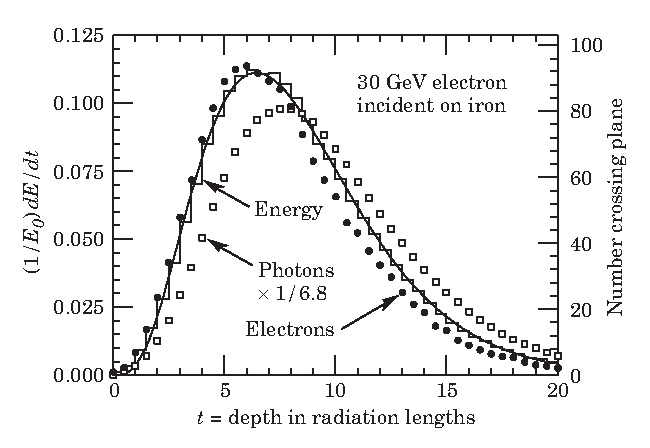
\includegraphics[width=0.65\textwidth]{photon/EMlong}}
\caption[Simulated longitudinal electromagnetic shower profile as a function of depth for electrons and photons.]
{An EGS4 simulation of a 30\,GeV electron-induced electromagnetic shower in iron. The histogram shows fractional energy deposition as a function of radiation lengths, and the curve is a gamma-function fit to the distribution. Circles and squares are the number of electrons and photons respectively with total energy greater than 1.5\,MeV crossing planes with scale on right. Plot is taken from \cite{Agashe:2014kda}.}
\label{fig:photonEMlongProfile}
\end{figure}

%The \RM of a material  describes the EM transverse  shower profile.
The EM transverse shower profile can be described as  a narrow cone widening as the shower develops. 90\% of the shower energy  is contained in a fiducial cylinder with a radius of one \RM, along the direction of the shower.

%%The dense shower core of the transverse profile allows the separation of two EM showers using a two-dimensional peak-finding algorithm, explained in a later section.



%Photon reconstruction is an important part of \pandora reconstruction. A good photon reconstruction should provide a good single photon completeness and purity, as well as a good photon separation resolution. For many physics processes, heavy particles decaying into photons, such as \Ptau lepton and \Ppizero. Photon reconstruction is crucial for reconstructing these heavy particles.

%The photon reconstruction presented in this chapter has improved the photon reconstruction completeness by reducing the fragments. The photon separation resolution has  also been improved. This work has been published in a conference proceeding \cite{Xu:2016rcz}. The improved  photon reconstruction has benefited many physics analyses involving photons. The most recent example is the  \HepProcess{\PHiggs \to \Pgamma \Pgamma} analysis at \rootS{3} at \CLIC \cite{Kacarevic:higgsToGammaGamma}.

%This set of photon related algorithms have been incorporated into the default reconstruction chain in \pandora. The \CLIC simulation studies have benefited from the improved photon reconstructions in various physics process, such as  \HepProcess{ \PHiggs \to \Pgamma \Pgamma}.

\begin{comment}
Since the discovery of a particle consistent with being the SM Higgs boson in LHC at 2012 \cite{Aad:2012tfa,Chatrchyan:2012ufa}, our understanding of Standard Model has improved greatly. Yet limited by the underlying QCD interaction from proton-anti-proton collision, one has great difficulty to measure the properties of the Higgs precisely. Next generation electron-positron linear collider could hopefully make precision measurements of the Higgs sector and the Top quark sector \cite{Abramowicz:2013tzc}.

The leading candidates for next generation electron-positron linear collider are the International Linear Collider (ILC) \cite{Brau:2007zza}, and the Compact Linear Collider (CLIC) \cite{Linssen:2012hp}. The ILC has developed two detector models, namely the International Large Detector (ILD) \cite{Abe:2010aa} and the Silicon Detector (SiD) \cite{Aihara:2010zz}. The CLIC has developed two slightly modified detector models based on ILD and SiD \cite{Linssen:2012hp}. One key common feature of these next generation electron-positron linear colliders is the high granular calorimeter, which provides a great spatial resolution at the cost of the energy resolution. Particle flow algorithms (PFA) benefit from the spatial resolution from calorimeters, together with tracking information, to provide excellent a jet energy resolution. PandoraPFA, the most complicated and the best performing one, provides a jet energy resolution of less than 3.5\%, which is required for W/Z separation \cite{Thomson:2009rp,Marshall:2013bda}.

\begin{figure}[tbph]
\centering
{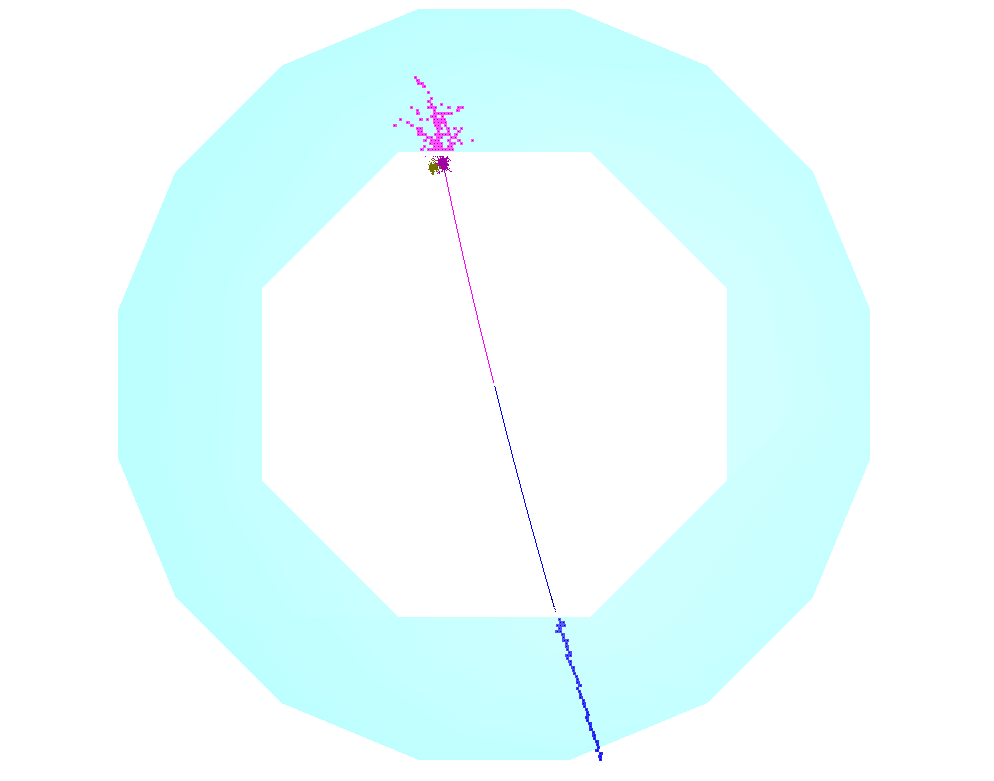
\includegraphics[width=0.5\textwidth]{images/tautauMod}}%

\caption{An event display of a simulated $\Pem\Pep\to \Ptauon\APtauon$ event. The blue region is the cross section of the Electromagnetic Calorimeter barrel region. The top $\Ptau$ decays into a charged $\Ppi$, two photons and neutrinos. The bottom $\Ptau$ decays into a muon and neutrinos.}
\label{fig:Tautau}
\end{figure}

Photon reconstruction is an important part of particle reconstruction. For many physics processes involving particles decaying into photons, such as $\Ptau$ lepton and $\Ppizero$, a good photon reconstruction, which provides a good single photon completeness and purity, as well as a good photon separation resolution, is crucial for reconstructing these particles.

\end{comment}

%\section{Electromagnetic shower}

\section{Overview of photon reconstruction in \pandora}

%\pandora is a multi-algorithm pattern-recognition software package for the event reconstruction and an implementation of the particle flow approach to calorimetry. A detailed discussion of the \pandora and the main steps of the \pandora event reconstruction can be found in \Section{sec:pandoraPandoraPFA}. The multi-algorithm approach of the \pandora allows each algorithm to deal with a particular issue in the reconstruction.


Five algorithms are developed to tackle different issues in the photon reconstruction. The most important photon algorithm is the \PhotonReconstruction algorithm. It reconstructs photons from calorimeter hits in the \ECAL, including forming a photon candidate and applying a photon ID test, with special treatments for photons close to charged particles. %This algorithm is implemented at the early stage of the reconstruction.


Three algorithms remove photon fragments at a later stage in the reconstruction. Two photon fragment removal algorithms merge fragments in the \ECAL, and one algorithm merges fragments in the \HCAL. The last photon algorithm is a photon splitting algorithm. The algorithm separates accidently merged photons.

%These algorithms improve the compsingle photon energy resolution.

%, which helps photon separation resolution.

%These algorithms together form the photon reconstruction in the \pandora. This chapter will first introduce the photon-induced electromagnetic shower in a calorimeter, followed by the description of each algorithm. The performance of the photon reconstruction will be provided in the last part of the chapter.

\begin{comment}
\pandora provides a framework for particle reconstruction \cite{Marshall:2015rfa}, as described in \Section{sec:pandoraPandoraPFA}. In the linear collider user case, it has a vast library of algorithms developed over years by many people. Each algorithm addresses one topological issue in the particle reconstruction. The essential part of the \pandora is track-cluster association  to find the best track-cluster pair, and re-clustering to find the best cluster consistent with the track. Other algorithms that identifies trackless clusters, such as muon clusters or photon clusters, would provide a cleaner environment for the track-cluster association, hence improving the jet energy resolution.

Photon identification in \pandora has two main mechanisms. The basic mechanism performs photon identification at the last step of the reconstruction  (see \Section{sec:pandoraPFOcreation}). The second more sophisticated photon identification is performed at an early stage of the reconstruction  (see \Section{sec:particleID}). The second algorithm identifies photon electromagnetic shower cores carefully in a dense jet environment. By removing photons from the environment, fewer calorimeters hits are left for charged particle reconstruction. Hence the overall reconstruction improves.

The \PhotonReconstruction algorithm in \pandora version 1 improves jet energy resolution by correctly identifying photon electromagnetic shower cores and leaving a cleaner environment for the track-cluster association. However, peripheral calorimeter hits to the shower cores may be reconstructed as separate particles (fragments). This lowers the reconstructed photon completeness and makes the number of reconstructed photons a less useful physical quantity. Also, the algorithm in \pandora version 1 leaves rooms for improvement of photon separation resolution.

This chapter presents a solution to photon reconstruction issues. The newly introduced algorithms reduces photon fragments and improves the photon separation resolution.

%Some part of the work has been published in a conference proceeding \cite{Xu:2016rcz}.

Firstly an overview of electromagnetic showers is presented. The \PhotonReconstruction algorithm will be described next, followed by fragment removal algorithms and photon splitting algorithms. This chapter will end with a discussion on performances of these photon related algorithms,  including comparisons with the previous photon algorithm.
%Algorithms related to photon reconstruction, fragmental removal and photon splitting, which are written or introduced by authors, will be discussed below.
\end{comment}

%The testing simulated data in this paper are generated either by WHIZARD \cite{whizard} or by the simple HepEvt generator. Events are simulated with GEANT4 \cite{Agostinelli:2002hh} in MOKKA \cite{MoradeFreitas:2002kj}. Jet fragmentation was performed with PYTHIA \cite{Sjostrand:1995iq} and the particle reconstruction was done by PandoraPFA \cite{Marshall:2015rfa} in MARLIN reconstruction framework \cite{Gaede:2006pj}, in ILD\_o1\_v6 detector model. The iLCSoft v17-01-07 was used. Different versions of PandoraPFA were used for the comparison purpose.




\section{\PhotonReconstruction algorithm}
\label{sec:photonRecostrcution}


The \PhotonReconstruction runs at an early stage of the reconstruction. It corresponds to ``Particle ID'' stage in the \pandora reconstruction, described in \Section{sec:particleID}.  Main steps of the \PhotonReconstruction algorithm, shown in \Figure{fig:photonPhotonRecoFlow}, are:  forming photon clusters; finding photon candidates; photon ID test; and optional fragments removal.

%Finding photon candidates uses the transverse EM shower profile information, which requires a  two dimensional peak finding algorithm, further explained in \Section{sec:peakFinding}. The photon ID test involves a multi dimensional likelihood classifier, which is described in \Section{sec:photonLikelihood}. The optional fragment removal algorithm shares a common code base case class with another photon fragment removal algorithm. Hence two photon fragment removal algorithms are discussed together in \Section{sec:photonFragRemoval}.

\begin{figure}[tbph]
\centering
{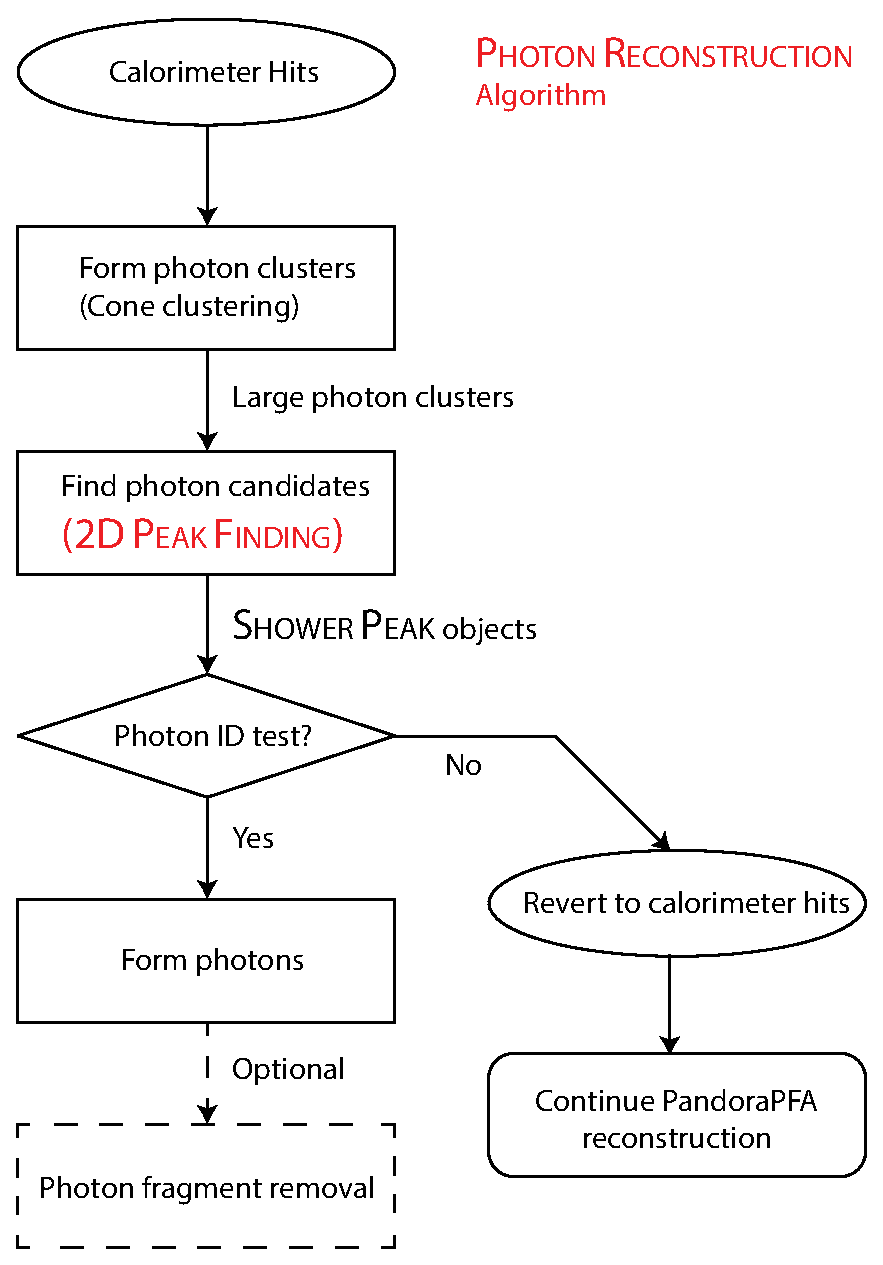
\includegraphics[width=0.65\textwidth]{photon/photonRecoFlow2}}
\caption[A flow diagram of the \PhotonReconstruction algorithm.]
{Main steps of the \PhotonReconstruction algorithm: forming photon clusters; finding photon candidates; photon ID test; and optional fragments removal.}
\label{fig:photonPhotonRecoFlow}
\end{figure}


\subsection{Forming photon clusters}

The inputs of the \PhotonReconstruction algorithm are calorimeter hits in the \ECAL that have not been used to form particles in previous algorithms. For example, muon reconstruction algorithms form muons and remove calorimeter hits associated with muons from the reconstruction. The  calorimeter hits associated with reconstructed muons are not used to form photons.

This step forms clusters from calorimeter hits in the \ECAL using the cone clustering algorithm. Since the target for reconstruction is the neutral photon, the cone clustering algorithm uses high-energy calorimeter hits in the \ECAL as initial seeds, instead of using track projections as initial seeds.  The clusters are formed in a way such that calorimeter hits from one photon would not be split into two clusters, but one cluster may contain calorimeter hits from  multiple photons.


%The algorithm uses  the cone clustering algorithm  provided inside \pandora to form clusters.   %The parameters for the cone clustering are such that  forming large clusters is preferred.

\subsection{Finding photon candidates}
\label{sec:photonCandiate}

This step refines photon clusters into smaller photon candidates. Each photon candidate should contain calorimeter hits from one photon only.

If a cluster contains calorimeter hits from several photons, the three-dimensional cluster will be split into several smaller clusters (photon candidates).

The three-dimensional splitting problem is harder than a two-dimensional one. Therefore, a translation is needed to map the three-dimensional problem to a more manageable two-dimensional problem. This translation relies on the characteristic EM transverse shower profile. Along the direction of the shower, an EM shower can be modelled as a dense shower core with peripheral calorimeter hits around the core. When the energies of the calorimeter hits of the cluster are projected onto a two-dimensional plane, an EM shower core would appear as a mountain-like structure in the plane. \FIGURE{fig:photonPeakFinding} shows an example of a photon cluster projected onto a two-dimensional plane, where two EM showers are identified. Hence, by identifying a peak in the two-dimensional plane, the EM shower core is identified.

%the energy deposition projection of two photons candidates. U and V axis are two arbitrary orthogonal axis in the transverse plane perpendicular to the direction of photons. Z axis shows the sum of the calorimeter hit energy in GeV. The bin size corresponds to the square \ECAL cell size.


%To reduce the problem of splitting a three dimensional clusters (a collection of hits) into a manageable two dimensional problem.

%The large photon clusters are split into smaller photon candidates, using two-dimensional shower profiles. The candidates close to a track projection are deemed as non-photons. Identifying photon candidates within a large photon cluster relies on the characteristic electromagnetic showers, in particular the transverse distribution. A energetic photon or electron hits the absorber layers of the \ECAL, it initiates an electromagnetic shower, where electron pair production and bremsstrahlung produce more low-energy photons and electrons. The transverse distribution is characterised by a narrow cone, widening while the shower develops.

%To view the transverse shower distribution, a two-dimensional energy deposition projection is constructed in the plane perpendicular to the direction of the cluster. \Figure{fig:photonPeakFinding} shows the energy deposition projection of two photons candidates. U and V axis are two arbitrary orthogonal axis in the transverse plane perpendicular to the direction of photons. Z axis shows the sum of the calorimeter hit energy in GeV. The bin size corresponds to the square \ECAL cell size.

\begin{figure}[tbph]
\centering
{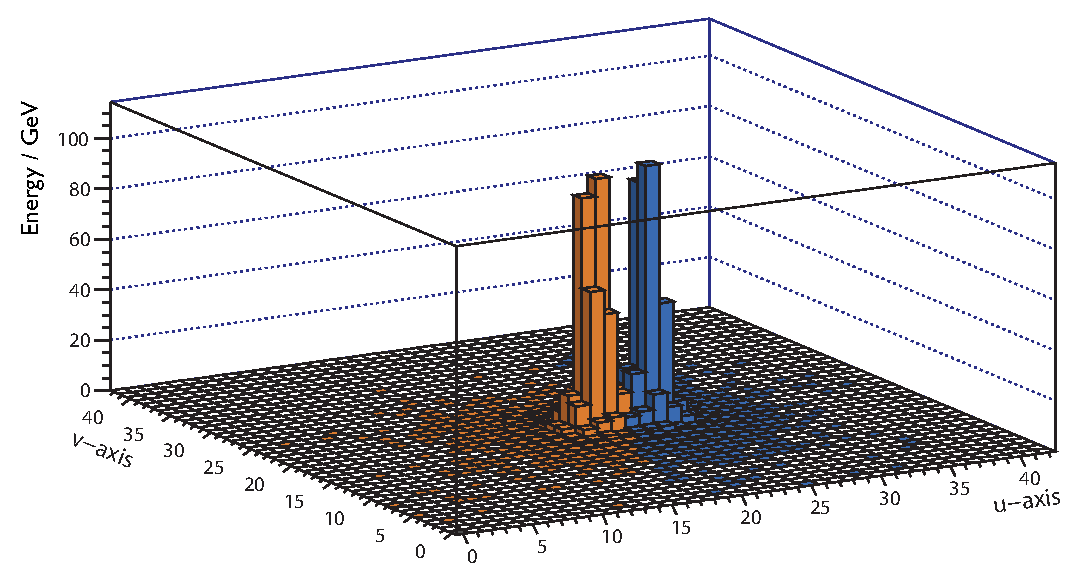
\includegraphics[width=0.7\textwidth]{photon/peakFindingMod}}
\caption[Example of projecting a large photon cluster containing two photons.]
{Two 500\,GeV photons (yellow and blue) within a  cluster, just resolved in a transverse plane orthogonal to the direction of the flight of the cluster.  The axes U and V are orthogonal axes in units of the \ECAL cell sizes. The height of a bin in the histogram is the sum of the calorimeter hit energy associated with the bin.}
\label{fig:photonPeakFinding}
\end{figure}

%obtained by projecting the energy deposition of the calorimeter hits of the cluster in the plane.

A high-performance two-dimensional peak-finding algorithm is the key to identify multiple photon candidates within a cluster. Due the complexity of the peak finding procedure, a peak-finding algorithm is developed and discussed in \Section{sec:peakFinding}. The output of the two-dimensional peak-finding algorithm is a collection of \ShowerPeak objects. Each \ShowerPeak object corresponds to one photon candidate and associated calorimeter hits.

\subsection{Photon ID test}
\label{sec:photonIDtest}

This step applies the photon ID test on the \ShowerPeak object. The photon ID test uses  a multidimensional likelihood classifier. A set of variables, which exploit features of electromagnetic showers, are used. The response from the classifier determines if a \ShowerPeak object is a photon. If it is a photon, the \ShowerPeak object would be tagged as a photon and the photon is not used in the subsequent event reconstruction. The identified photon re-enters the event reconstruction at the fragment removal stage. If a \ShowerPeak object   fails the  photon ID test, the \ShowerPeak object  will be discarded. Calorimeter hits associated with discarded the \ShowerPeak object will be passed onto the next stage of the reconstruction. The likelihood classifier used in the photon ID test is further discussed in \Section{sec:photonLikelihood}.

\subsection{Photon Fragment removal}
\label{sec:photonRecoFragRemoval}

The  photon fragment removal algorithm merges small photon fragments to identified photons. The algorithm is optional as it is not used by the default setting of the event reconstruction. Since this algorithm shares the same logic as another fragment removal algorithm, two algorithms are discussed togethers in \Section{sec:photonFragRemoval}.

%only differing in the cut-off values for merging metrics, this step be discussed in \Section{}.

This step marks the end of the \PhotonReconstruction algorithm. The outputs are reconstructed photons, separated from non-photon calorimeter hits.
%The candidate passed the test will be kept in a separate container for photons only

\section{\peakFinding algorithm}
\label{sec:peakFinding}

As discussed in \Section{sec:photonCandiate}, identifying photon candidates inside a cluster is translated into identifying peaks in a two-dimensional plane, using a two-dimensional peak-finding algorithm (\peakFinding algorithm). The \peakFinding algorithm aims to correctly identify peak positions in a two-dimensional histogram and to associate calorimeter hits of non-peak bins to identified peaks.

% An example of two photons resolved in a two dimensional plane is shown in the \Figure{fig:photonPeakFinding}.

There are two variants of the \peakFinding algorithm: the neutral cluster variant and the charged cluster variant. The base algorithm is  the neutral cluster variant. The charged cluster variant is used when the cluster is close to the projection of a track onto the front of the \ECAL. Main steps of the  neutral cluster variant are shown in \Figure{fig:photonPeakFindingFlowNeutral}: initialising a two-dimensional histogram; projecting  calorimeter hits to the histogram; identifying local peaks; associating non-peak bins to peaks; filtering peaks; and forming \ShowerPeak objects.

%Since charged hadrons would deposit tracks in the tracking system, extra care is taken when a cluster is close to the projection of the track in the front of the \ECAL.

% The neutral cluster variant is described first, followed by description of the modification of the algorithm to treat clusters close to track projections.

\begin{figure}[tbph]
\centering
{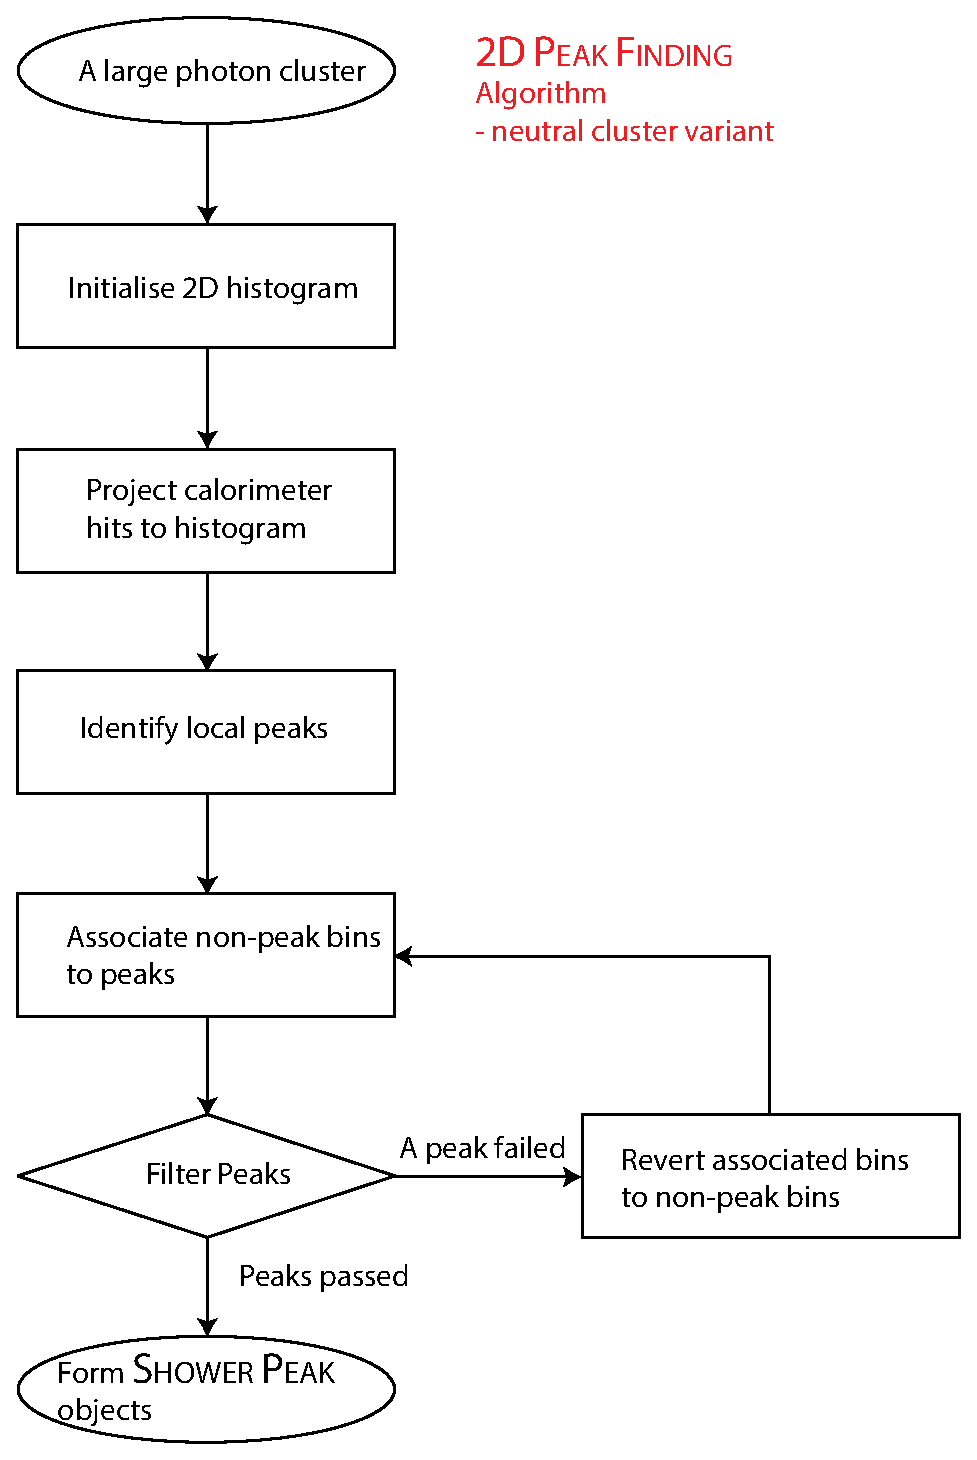
\includegraphics[width=0.7\textwidth]{photon/2DpeakFinding2}}
\caption[Flow chart for \peakFinding algorithm neutral cluster variant.]
{Main steps of the  neutral cluster variant of the \peakFinding algorithm: initialising a two-dimensional histogram; projecting  calorimeter hits to the histogram; identifying local peaks; associating non-peak bins to peaks; filtering peaks; and forming \ShowerPeak objects.}
\label{fig:photonPeakFindingFlowNeutral}
\end{figure}

\subsection{Initialising  two-dimensional histogram}

This step initialises a two-dimensional (2D) histogram to host the projection of the calorimeter hits of the cluster. For the best resolving power between EM showers, the projection direction is chosen to be the direction of the cluster. Two axes of the two-dimensional histogram are chosen such that the axes and the direction of the cluster form an orthogonal basis  in the three-dimensional space.

%The axes are labelled as  U and V axis in \Figure{fig:photonPeakFinding}.



\subsection{Projecting calorimeter hits to histogram}

%For a finite-sized 2D histogram, t
This step projects the calorimeter hits associated with the cluster onto the 2D histogram. The projection is chosen such that the cluster centroid position is projected onto the centre of the histogram. The distance between the calorimeter hit position and the cluster centroid position is converted into a distance vector to be used to project the calorimeter hit. The distance vector, $\vec{s_{i}}$, of a calorimeter hit $i$, is defined as:
\begin{equation}
\vec{s_{i}} = \frac{\vec{a_{i}} -  \vec{\angles{a}}}{d_{cell}},
\end{equation}
where $\vec{a}$ is the three-dimensional position of the calorimeter hit $i$;  $\vec{\angles{a}}$ is the centroid position of cluster $a$; and $d_{cell}$ is the  \ECAL square cell length. The coordinate of the calorimeter hit projection onto the histogram is calculated from the scalar products of the distance vector ($\vec{s_{i}}$) with the axes vectors.
% One bin size along either axes on the 2D histogram corresponds to one \ECAL square cell length.

The height of a bin in the 2D histogram is the sum of the energies associated with the calorimeter hits that fall in that particular bin. Each bin contains calorimeter hits that projected onto the bin. One bin size along either axes on the 2D histogram corresponds to one \ECAL square cell length.

%The issue with the histogram size being finite is discussed in \Section{sec:photonPeakFindingInclusive}.

\subsection{Identifying local peaks}

This step identifies all local peaks in the 2D histogram. A local peak is defined as a bin where its height is above all eight neighbouring bins. All bins in the 2D histogram are  iterated to identify all local peaks. %Hence the processing time is $O\left(N^2\right)$, where $N$ is number of bins in one axis.
%For example, in \Figure{fig:photonPeakFinding}, there are clearly two peaks, both colour coded.
\subsection{Associating non-peak bins to peaks}

Having identified all local peaks, this step associates non-peak bins to a particular peak based on the energy of the peak and the distance of the non-peak bin to the peak bin. A non-peak bin should be associated to a high-energy peak bin that is close to the non-peak bin.

%The energy dependence is needed as the transverse EM shower width increases with the increase of the energy of the EM shower. The distance dependence is needed because the EM showers have dense shower cores, and
%To associate non-peak bins to the correct peak bin, the peak bin is
%The peak bin to associate a non-peak bin is chosen by minimising the metric:
A non-peak bin is associated with the peak bin that gives the smallest value of the metric:
\begin{equation}
\frac{d_{i}}{\sqrt{E_{i}}}
\end{equation}
where $d_{i}$ is the Euclidean distance between a non-peak bin and a  peak bin $i$ on the 2D histogram, and $E_{i}$ is the height (energy) of the peak bin $i$. For each non-peak bin, the metric is iterated over all peak bins to find the peak bin that produces the smallest metric. %Alternative metrics provided in the algorithm include $d_{i}$, $\frac{d_{i}}{{E_{i}}}$, and $\frac{d_{i}}{{E_{i}^2}}$. The default metric is chosen due to a good balance between distance and energy of the peak.

%And EM shower is typically narrow transversely.

\subsection{Filtering peaks}

The performance of the \peakFinding algorithm is improved by peak filtering. In a 2D histogram, such as the one in \Figure{fig:photonPeakFinding}, major peaks with many associated non-peak bins correspond most likely  to physical photons, while minor peaks with few associated non-peak bins are more likely from fluctuations in the energy deposition of the EM shower. To select only major peaks and to discard minor peaks, every time after all non-peak bins are associated with peak bins, peaks with fewer than three bins associated (including the peak bin) are discarded. These discarded bins are re-associated with other peak bins. This  process iterates until all peak bins have at least three bins associated.

%The peak filtering step also allows bins with heights below a critical value to not participate in the peak finding. The default value is set such that only non-empty bins are used.

After  filtering peaks,  \ShowerPeak  objects are created . One \ShowerPeak object contains one peak bin and associated non-peak bins. The associated calorimeter hits within the bins are attached to the \ShowerPeak object as well. If multiple peaks are identified in a cluster, multiple \ShowerPeak objects are created as outputs.

%This marks the end of the neutral clusters variant of the \PhotonReconstruction algorithm, outlined in \Figure{fig:photonPeakFindingFlowNeutral}.

%The  \ShowerPeak object is also referred to as the photon candidate.

\subsection{\peakFinding algorithm charged cluster variant}
\label{sec:photon2Dtrack}

In a dense jet environment, if a photon next to a charged hadron is carefully reconstructed, the charged particle reconstruction is improved.

%If  a photon candidate is close to the projection of the track onto the front of the \ECAL, it is more likely that the candidate is a charged hadron. Misidentifying a charged hadron as a photon leads to a significant degradation in the reconstruction performance, because there will be double counting of energies from the track and from the charged hadron misidentified as a photon. However,


This step aims to carefully identify photon candidates next to charged hadrons, by using track information and features of EM showers. An EM shower typically starts in the first few layers of the \ECAL with  direction of the EM shower largely unchanged when the shower develops.


\FIGURE{fig:photonPeakFindingFlow} shows the main steps in the full \peakFinding algorithm, including the treatment of clusters close to tracks. The "Close to track" step determines if a cluster is close to a track. If the distance between a cluster and the closest track projection onto the front of the \ECAL is fewer than 3\,mm, the charged cluster variant of the \peakFinding algorithm is applied to the cluster.

\begin{figure}[tbph]
\centering
{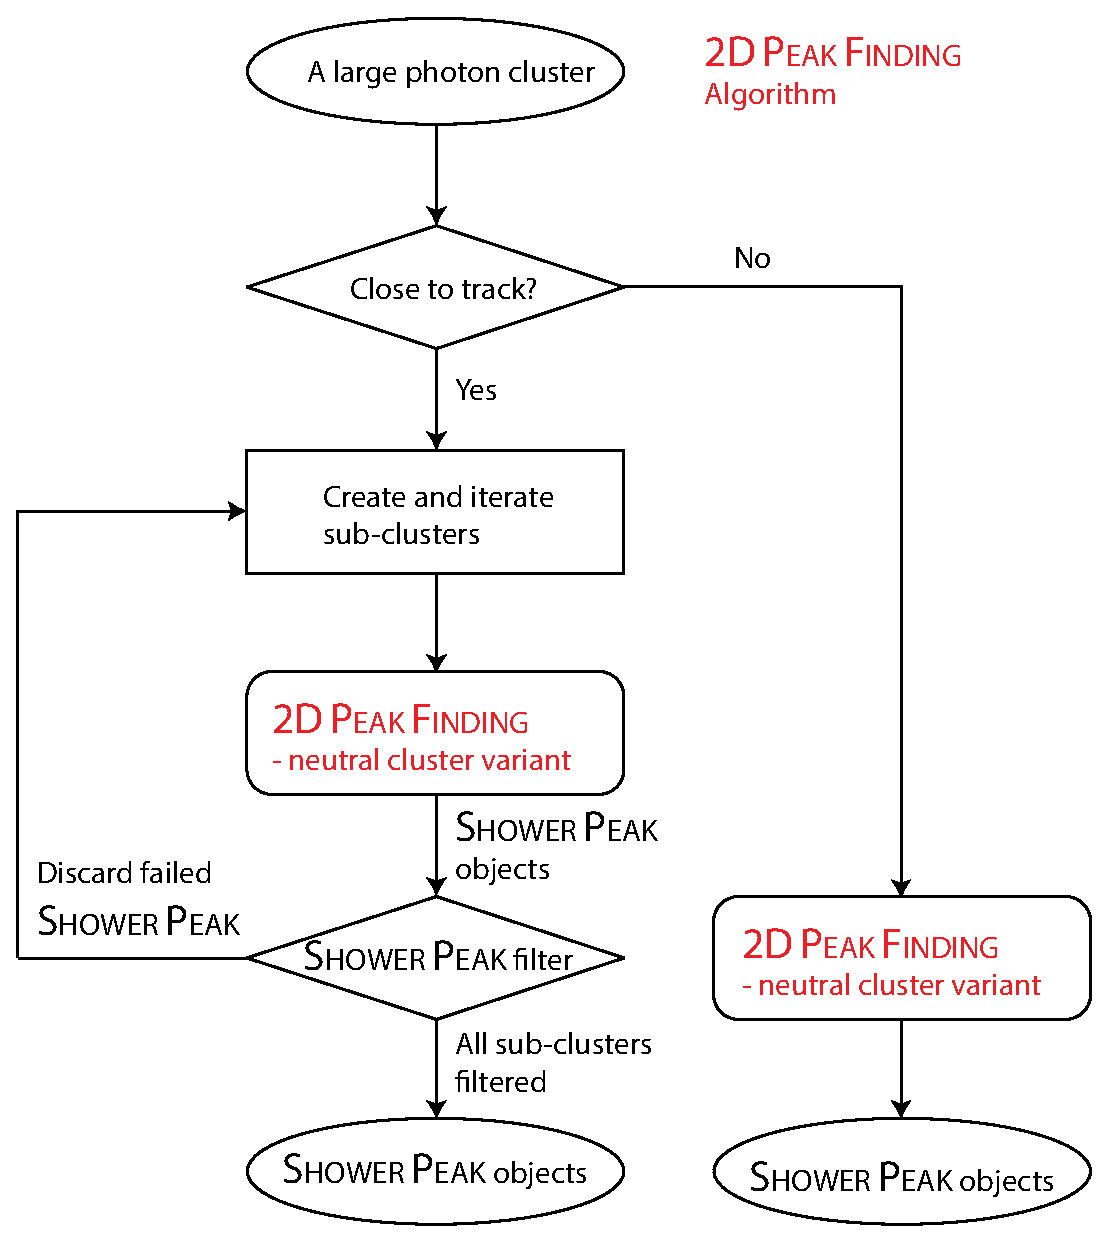
\includegraphics[width=0.8\textwidth]{photon/2DpeakFindingTrack}}
\caption[Flow chart for \peakFinding algorithm.]
{Main steps of the  \peakFinding algorithm, including the charged cluster variant: identifying whether the cluster is close to a track; creating and iterating over sub-clusters; applying \peakFinding algorithm neutral cluster variant to sub-clusters; filtering \ShowerPeak objects in sub-clusters; creating final \ShowerPeak objects.}
\label{fig:photonPeakFindingFlow}
\end{figure}


The "Create and iterate over sub-clusters" step performs the following. The \ECAL is sliced longitudinally to create fiducial volumes. For example, the default three slices will result in three \ECAL fiducial volumes. Each fiducial volume covers the  space from the front of the \ECAL to a third, to two thirds, and to the back of the \ECAL. Three sub-clusters are created from calorimeter hits that are contained in each fiducial volume.

After creating sub-clusters, the neutral cluster variant of the  \peakFinding algorithm is applied to each sub-cluster to find peaks.  The sub-cluster in the first third of the \ECAL is processed first. The sub-cluster in the whole of the \ECAL is processed last. For each sub-cluster, a collection of \ShowerPeak objects are created from the  \peakFinding algorithm.

The \ShowerPeak objects created from each sub-cluster undergo the "\ShowerPeak filter" step. The order of the \ShowerPeak objects to filter peaks is the same order of applying the neutral cluster variant of the  \peakFinding algorithm. All peaks from the first sub-cluster are preserved. For the next sub-cluster, a peak  is only preserved if the peak bin position is the same as a peak bin position in the previous sub-cluster, allowing a shift in the peak bin position by no more than one neighbouring bin. Furthermore, if a peak bin is within one neighbouring bin of a track projection bin, the peak is discarded. Only the peaks in the last sub-cluster that are preserved in every sub-cluster through the iteration of "\ShowerPeak filter" step will be used to form the final \ShowerPeak objects. The track projection bin in the 2D histogram is where position of the track projection onto the front of the \ECAL projects onto the 2D histogram.

%The track projection bin is obtained by projecting the position to the 2D histogram.
% of the track projection onto the front of the \ECAL
%The non-preserved peak and the associated \ShowerPeak object are discarded.

\FIGURE{fig:photon2DpeakCharge} illustrates an example of three sub-clusters created during the charged variant of the \peakFinding algorithm, reconstructed using the \ILD detector model. Peaks, associated bins, and track projection bins are labelled. \FIGURE{fig:photon2DpeakCharge1} shows the first sub-cluster, created with calorimeter hits in the first 10 layers of the \ECAL. One peak is identified. \FIGURE{fig:photon2DpeakCharge2} shows the second sub-cluster, created with calorimeter hits in the first 20 layers of the \ECAL. The one peak in the second sub-cluster is in the same position of the peak in the first sub-cluster. Hence, the peak in the second cluster is preserved. \FIGURE{fig:photon2DpeakCharge3} shows the third sub-cluster, created with calorimeter hits in the \ECAL. Three peaks are identified. However, only one peak (blue) shares the  same position of the peak in the second sub-cluster. Hence, only that peak (blue) is preserved. The preserved peak and associated bins in the third sub-cluster are then used to create one \ShowerPeak object.


\begin{figure}[tbph]
\centering
  \begin{subfigure}[b]{0.65\textwidth}
    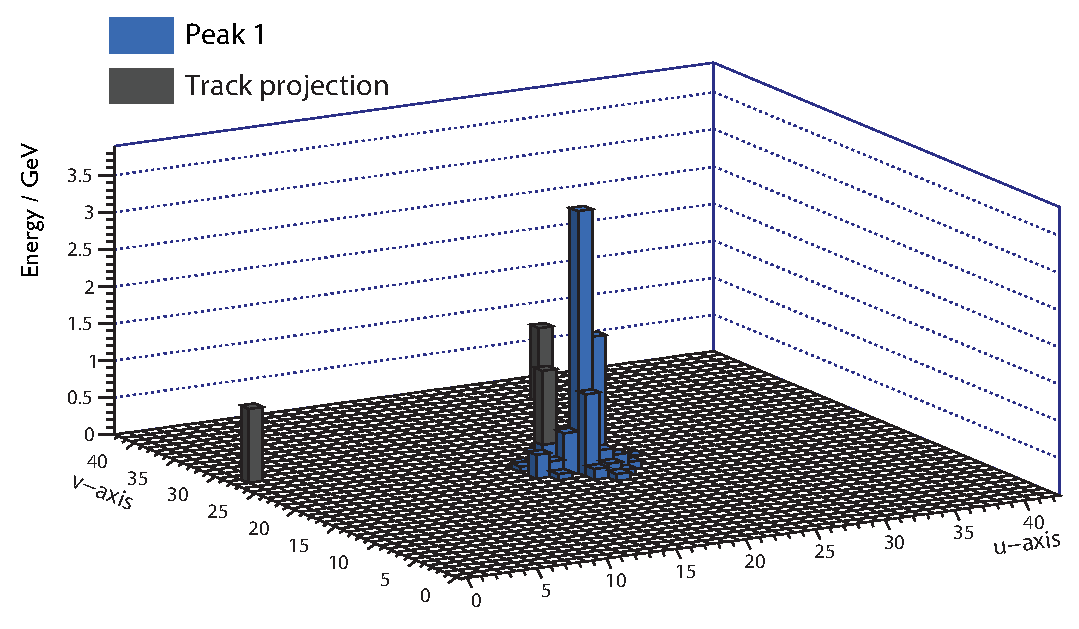
\includegraphics[width=\textwidth]{photon/2Dpeak/charge1}
    \caption{}
    \label{fig:photon2DpeakCharge1}
  \end{subfigure}
  \begin{subfigure}[b]{0.65\textwidth}
    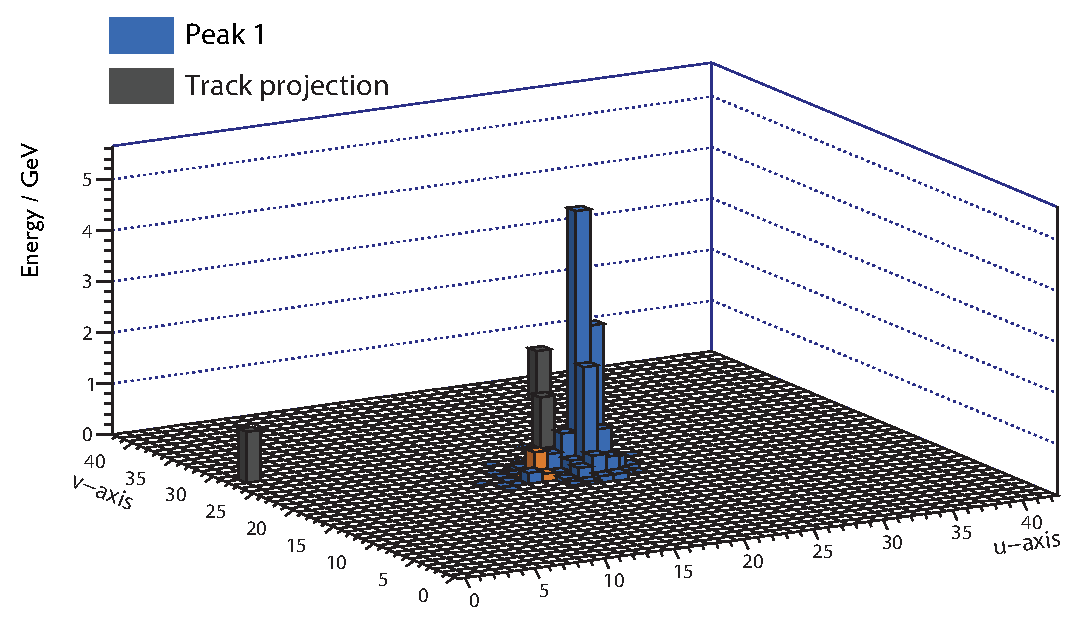
\includegraphics[width=\textwidth]{photon/2Dpeak/charge2}
    \caption{}
    \label{fig:photon2DpeakCharge2}
  \end{subfigure}
  \begin{subfigure}[b]{0.65\textwidth}
    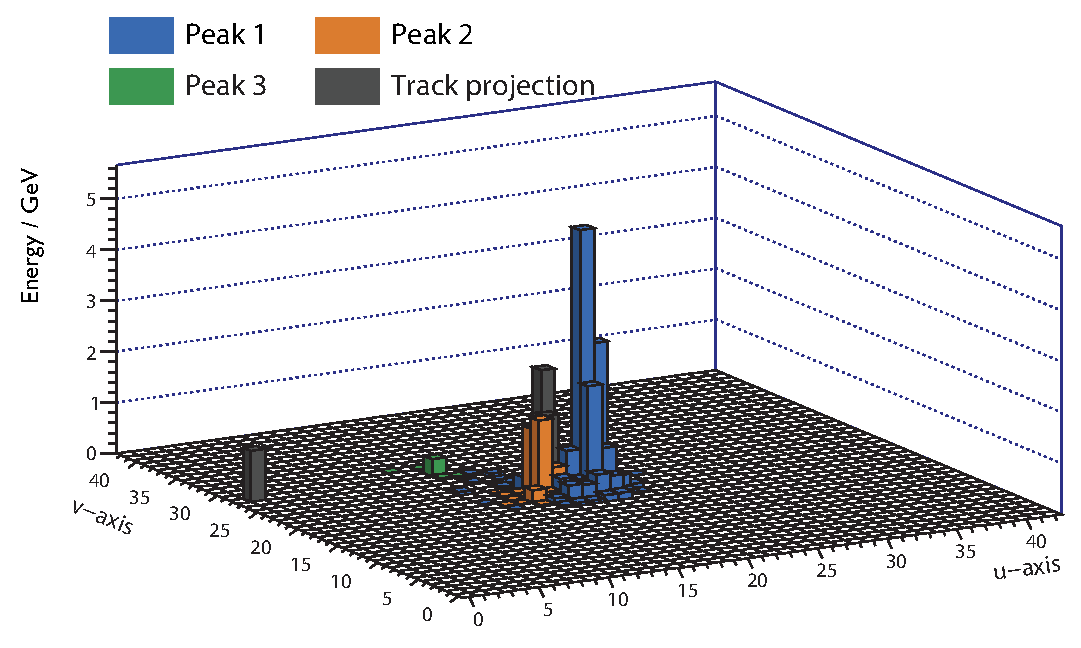
\includegraphics[width=\textwidth]{photon/2Dpeak/charge3}
    \caption{}
    \label{fig:photon2DpeakCharge3}
  \end{subfigure}
\caption
{An illustration of three sub-clusters created during the charged cluster variant of the \peakFinding algorithm. Peaks, associated bins, and track projection bins are labelled.}
\label{fig:photon2DpeakCharge}
\end{figure}


\subsection{Inclusive mode}
\label{sec:photonPeakFindingInclusive}

%The 2D histogram is iterated many times during the algorithm.

The time complexity of iterating the 2D histogram is $O(n^2)$ for a $n$ bins by  $n$ bins sized histogram (default $n = 41$). Therefore, for the purpose of speed, it is undesirable to have  a large number of bins. Having a small finite-sized histogram speeds up the computation. However, because of the finite size of the histogram, only  calorimeter hits  projected onto the histogram would be considered by the peak finding algorithm. Calorimeter hits projected outside the histogram would not be used when \ShowerPeak objects are constructed. This behaviour is suitable if the algorithm is only interested in finding the EM shower cores, for example, the \PhotonReconstruction algorithm. However, for the purpose of photon splitting, all calorimeter hits from the parent photon should be used to form daughter photons. Hence the inclusive mode of the \peakFinding algorithm is developed, and allows calorimeter hits projected outside the histogram to be associated with identified peaks.


\section{Likelihood classifier for photon ID test}
\label{sec:photonLikelihood}

In \Section{sec:photonIDtest}, the photon ID test in the photon reconstruction algorithm is outlined. This section describes the multidimensional likelihood classifier used in the photon ID test in details.
%For each photon candidate, a set of variables are calculated and used to as inputs to the classifier.

%\subsection{Overview of Projective Likelihood}
%\label{sec:photonPDE}

\subsection{Likelihood classifier variables}

Variables used in the likelihood classifier exploit the differences between a characteristic electromagnetic shower and a hadronic shower, and the fact that a photon is less likely to be close to track projections onto the front of the \ECAL, than a cluster of a charged particle. Variables used in the classifier are listed in \Table{tab:photonPhotonIDvar}.

Two variables are obtained from the EM longitudinal shower profile: the variable $t_0$ is the start layer from the longitudinal shower profile, shown in \Figure{fig:photonLongProfileStart}; and $\delta{l}$ is fractional difference of the observed shower profile to the expected EM shower profile described in \Equation{eq:photonEMshower}:
\begin{equation}
\delta l = \frac{1}{E_0}\sum_{i}^{}\absOf{\Delta E_{obs}^i - \Delta E_{EM}^i },
\end{equation}
where $E_0$ is the energy of the EM shower; $\Delta E_{EM}^i$ is the energy of the expected EM shower profile in bin $i$;  $\Delta E_{obs}^i$ is the energy of the observed EM shower profile in bin $i$; the index $i$ is summed over the \ECAL layers as the EM shower is binned according to the \ECAL layers; and the quantity $\delta l$ is minimised as a function of the $t_0$. The $\delta l$ distributions for photons and non-photons are shown in \Figure{fig:photonLongProfileDiscrepancy}. For a true photon, $t_0$  and $\delta l $ are expected to be small, as an EM shower should start in the first few layers of the \ECAL and the shower profile should be similar to an expected EM shower profile.

Three variables are obtained from the transverse EM shower profile: the variable $\langle{w}\rangle$ is the energy weighted \rms distance of all bins in a \ShowerPeak to its peak bin, a measure of the transverse shower size, shown in \Figure{fig:photonPeakRms}; the variable $\delta{\langle{w_{UV}}\rangle}$ is the smallest ratio of the two energy weighted \rms distances of all bins in a \ShowerPeak to its peak bin in each of the U, V axis direction, a measure of the circularity of the transverse shower; the last variable, $\delta E_{cluster}$, is the  ratio of the energy of the \ShowerPeak object to the cluster energy, a measure of the dominance of a \ShowerPeak in a cluster.

The last variable used in the classifier, $d$, is the distance between the candidate and the closest track projection onto the front of the \ECAL. The \ShowerPeak object is less likely to be a photon if it is close to a track. The distributions for photons and non-photons are shown in \Figure{fig:photonMinDistanceToTrack}.


\begin{table}[htbp] \centering \smallskip
\begin{tabular}{l r }
\hline
\hline
Categories&  Variables\\
\hline
EM longitudinal  shower profile & $\delta{l}$, $t_0$ \\
EM transverse  shower profile & $\langle{w}\rangle$, $\delta{\langle{w_{UV}}\rangle}$, $\delta E_{cluster}$ \\
Distance to track &  $d$ \\
\hline
\hline
\end{tabular}
\caption
{Variables used in the likelihood classifier for photon ID test.}
\label{tab:photonPhotonIDvar}
\end{table}

\begin{figure}[tbph]
\centering
  \begin{subfigure}[b]{0.45\textwidth}
    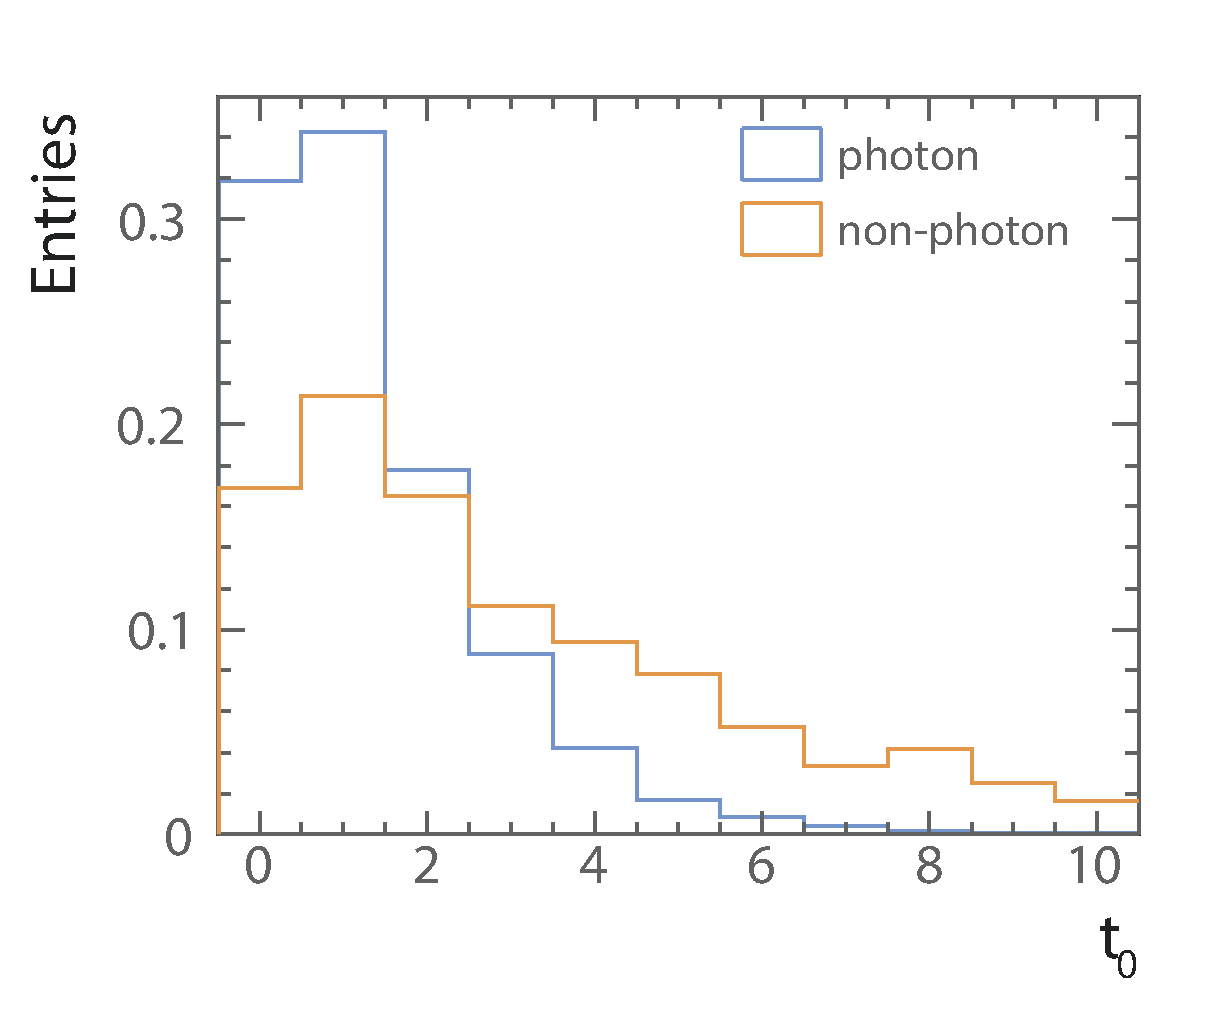
\includegraphics[width=\textwidth]{photon/likelihood/LongProfileStart2}
    \caption{}
    \label{fig:photonLongProfileStart}
  \end{subfigure}
  \begin{subfigure}[b]{0.45\textwidth}
    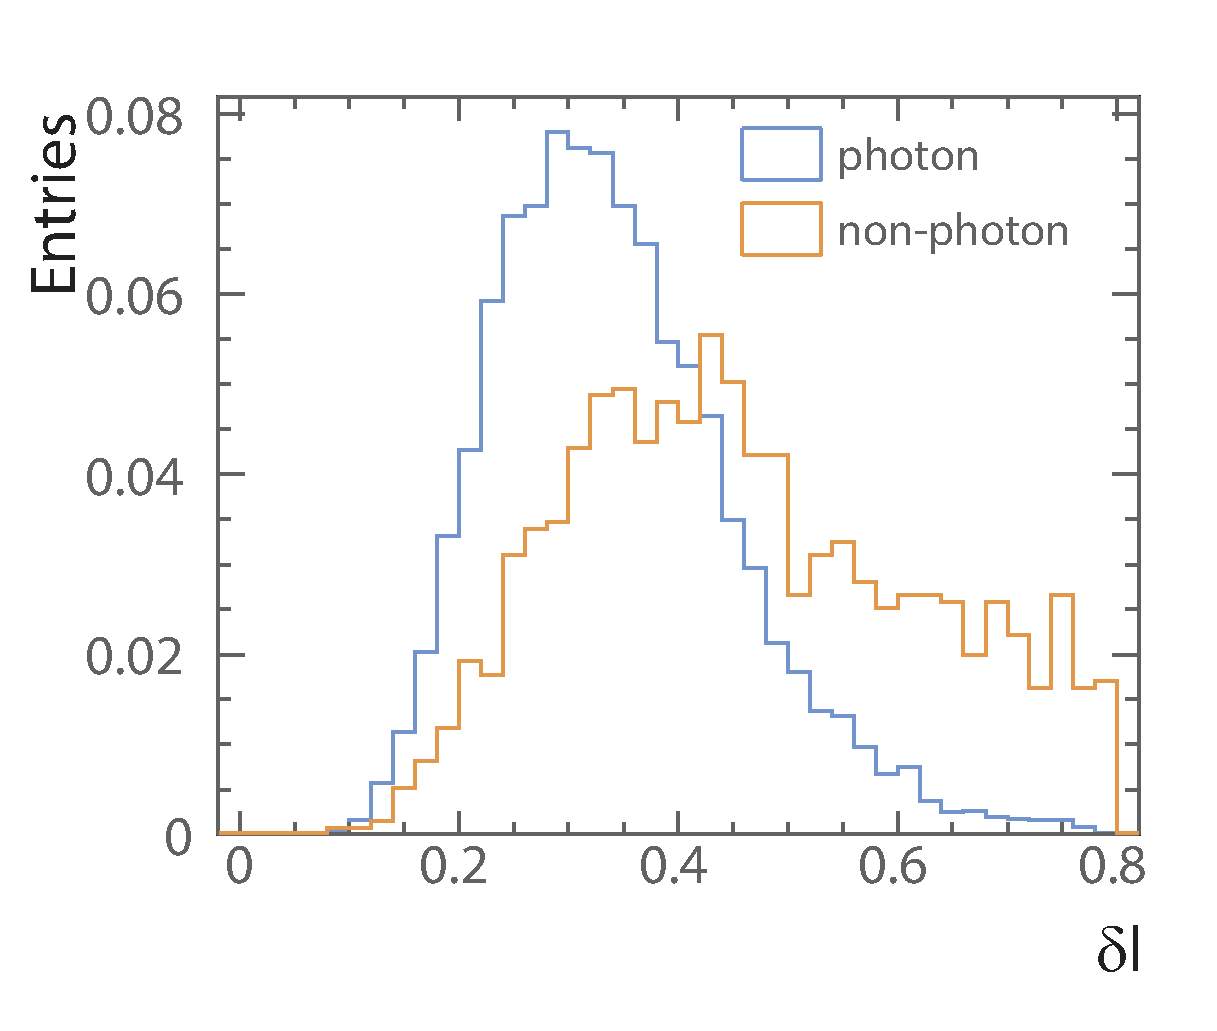
\includegraphics[width=\textwidth]{photon/likelihood/LongProfileDiscrepancy2}
    \caption{}
    \label{fig:photonLongProfileDiscrepancy}
  \end{subfigure}
  \begin{subfigure}[b]{0.45\textwidth}
    \includegraphics[width=\textwidth]{photon/likelihood/PeakRms2}
    \caption{}
    \label{fig:photonPeakRms}
  \end{subfigure}
  \begin{subfigure}[b]{0.45\textwidth}
    \includegraphics[width=\textwidth]{photon/likelihood/MinDistanceToTrack2}
    \caption{}
    \label{fig:photonMinDistanceToTrack}
  \end{subfigure}
\caption
{Distributions for a) the start layer from the longitudinal shower profile ($t_0$), b)  the fractional difference of the observed shower profile to the expected EM shower profile ($\delta{l}$), c) the energy weighted \rms distance of all bins in a \ShowerPeak to its peak bin ($\langle{w}\rangle$), and d) the distance between the photon candidate and the closest track projection onto the front of the \ECAL ($d$). The area under each curve is normalised to unity. The particle ID is determined using the truth information. All plots are produced with  simulated \eeZuds, at \rootSGeV{500}.}
\label{fig:photonVarLikelihood}
\end{figure}



%  Candidate with energy below 0.2\,GeV would not be examined in this step, as there are far more non-photons than photons and the classifier makes mor.

\subsection{Projective Likelihood classifier}


Projective likelihood classifier  with probability density estimators is used  for the photon ID test due to its  low requirement on computing resources, comparing to a boost decision tree classifier or a neutral network classifier.

The probability distributions of each variable for photons and non-photons are obtained in the training stage. The distributions of these variables are normalised to probability distribution, stored in binned histograms. The classifier is improved by realising the variable distributions varies with photon energies. Thus the variables distributions are stored separately for different photon energy ranges. There are 8 photon energy ranges, obtained by binning the distribution of photon energies at 0.2, 0.5, 1, 1.5, 2.5, 5, 10, 20\,GeV. The variable distributions for non-photon are binned in the same energy ranges, according to the energy of the non-photon.

The training stage of the classifier uses simulated  \eeZuds, at a centre-of-mass energy of 500\,GeV. The events at centre-of-mass energy of 500\,GeV allow the training of photon with energies greater than 20\,GeV.

%Thus these distributions are divided by a range of photon energies. The default energy bins edges are

In the applying stage of the classifier, for a given candidate with the candidate energy in the  energy bin $\alpha$, the classifier output is given by
\begin{equation}
\uprightMath{PID_\alpha} = \frac{N \prod_{i}^6{P_{i}}}{N \prod_{i}^6{P_{i}} + N' \prod_{i}^6{P'_{i}}}
\end{equation}
where $P_{i}$ and $P'_{i}$ are the probabilities of the candidate fallen in the  respective photon and non-photon $i^{th}$ variable probability distributions  in the energy bin $\alpha$; the variables $N$ and $N'$ are the number of respective photons and non-photons in the energy bin $\alpha$ in the training sample.


During applying stage of the classifier, a candidate passes the photon ID test if
\begin{equation}
\begin{cases}
  \text{PID} > 0.6, & \text{if}\ 0.2 < E < 0.5\,\text{GeV}\\
  \text{PID} > 0.4, & \text{if}\ E \geqslant 0.5\,\text{GeV}
\end{cases}
\end{equation}
where $E$ is the candidate energy. Two values of the cuts on $\text{PID}$ is because it is more likely to misidentify a low-energy particle as a photon. A low-energy EM shower does not have a dense shower core, and is more difficult to identify. Hence for candidates with energy between 0.2 and 0.5\,GeV, \uprightMath{PID > 0.6} is required instead of \uprightMath{PID > 0.4}.

%An EM shower from a high-energy photon is more distinct than the hadronic shower from a non-photon of the same energy, than the difference between a low-energy  EM shower and hadronic shower.

%reflect the different confidence levels of the photon ID test with different candidate energies.

%The test is more cautious with low-energy candidates.


\section{Photon fragment removal algorithm in the \ECAL}
\label{sec:photonFragRemoval}
During the reconstruction, it is possible that a core of the photon electromagnetic shower is identified as a photon (the main photon), but the outer part of the shower is reconstructed as a separate particle (the fragment), and identified as a photon or a neural hadron. \FIGURE{fig:photonEvtDspPhotonFrag} shows a typical creation of such a photon fragment, reconstructed with \pandora version 1. A fragment typically does not have the electromagnetic shower structure, and has a much lower energy than a main photon.

%If a photon$-$fragment pair is correctly merged, the pair should be consistent with properties of a single particle.

\begin{figure}[tbph]
\centering
  \begin{subfigure}[b]{0.3\textwidth}
    \includegraphics[width=\textwidth]{photon/allPhoton}
    \caption{}
    \label{fig:photonEvtDspPhotonFragAll}
  \end{subfigure}
  \begin{subfigure}[b]{0.3\textwidth}
    \includegraphics[width=\textwidth]{photon/big}
    \caption{}
    \label{fig:photonEvtDspPhotonFragBig}
  \end{subfigure}
  \begin{subfigure}[b]{0.3\textwidth}
    \includegraphics[width=\textwidth]{photon/small}
    \caption{}
    \label{fig:photonEvtDspPhotonFragSmall}
  \end{subfigure}
\caption
{An event display of a) a typical 10\,GeV photon, reconstructed into  b) a main photon,  and c) a photon fragment. }
\label{fig:photonEvtDspPhotonFrag}
\end{figure}

There are two variants of the photon fragment removal algorithms: one immediately after the \PhotonReconstruction algorithm, and the other one after the charged particle reconstruction. Since two algorithms share same logics for merging, the algorithm used   after the charged particle reconstruction will be discussed in detail here.

% can exist at difference places in the reconstruction:


% where cuts are developed by comparing photon$-$fragment pairs and non-photon$-$fragment pair using the truth information.
% Kinematic and topological properties of a photon$-$fragment pair are examined.
A photon and a fragment form a photon$-$fragment pair.  The pair is merged when its properties pass a set of cuts. Depending on whether the fragment is reconstructed as a photon or a neutral hadron, the photon$-$fragment pairs is further classified into photon$-$photon-fragment pairs and photon$-$neutral-hadron-fragment pairs. The pairs are subsequently  divided into low energy and high energy pairs, depending on whether the fragment energy ($E_f$) is above 1\,GeV. \FIGURE{fig:photonFragEnergy} shows the energies of the second most energetic reconstructed photons in the pair for the photon$-$photon-fragment pairs, the true photon$-$photon pairs, photon$-$neutral-hadron-fragment pairs, and true photon$-$neutral-hadron pairs. Events were generated with \eeZuds, at \rootSGeV{500}, reconstructed with the \pandora version 1. Most photon and neutral hadron fragments have energies below than 1\,GeV. Hence the energy sub-division was chosen to be at 1\,GeV.

\begin{figure}[tbph]
\centering
  \begin{subfigure}[b]{0.45\textwidth}
    \includegraphics[width=\textwidth]{{photon/frag/Photon_e_2_pp}}
    \caption{}
    \label{fig:photonFragPhotonEnergy}
  \end{subfigure}
  \begin{subfigure}[b]{0.45\textwidth}
    \includegraphics[width=\textwidth]{{photon/frag/Photon_e_2_pn}}
    \caption{}
    \label{fig:photonFragNeutralEnergy}
  \end{subfigure}
\caption
{The energies of the second most energetic reconstructed photons in the pair, for a) the photon$-$photon-fragment pairs, and the true photon$-$photon pairs , and for b) the  photon$-$neutral-hadron-fragment pairs, and the true photon$-$neutral-hadron pairs. Events were generated with \eeZuds, at \rootSGeV{500}, reconstructed with the \pandora version 1.}
\label{fig:photonFragEnergy}
\end{figure}


% , because they have different kinematic and topological distributions.
% $d$, $d_c$ and $d_h$ are mean energy weighted intra-layer distance within the pair, distance between two centroids, and minimum distance between calorimeter hits of each \PFO in the pair, respectively.  Three distance measurements have subtle difference.
\TABLE{tab:photonFragRemovalCuts} lists cuts for merging photon$-$photon-fragment pairs and photon$-$neutral-hadron-fragment pairs for both low energy and high energy fragments. The description of each variable used in the cuts will be provided first, followed by the description of the logics of the cuts.

\subsection{Variables}

There are three distance variables: the variable $d_c$ gives the distance between centroids of the particles in the photon$-$fragment pair, which is a computationally quick measurement;  the variable  $d_h$ is the minimum distance between calorimeter hits of each particle in the photon$-$fragment pair;  the variable  $d$ is the average energy weighted intra-layer distance between  two particles in the photon$-$fragment pair, illustrated schematically in \Figure{fig:photonDistanceMetric}:
\begin{equation}
d = \frac{\sum_{i}^{layers}d_l^i \ E_{f}^i}{\sum_{i}^{layers}E_{f}^i}
\end{equation}
where index $i$ indicates $i^{th}$ layer of the \ECAL; the parameter $d_{l}^i$ is the minimum distance between calorimeter hits of the photon and the fragment in the $i^{th}$ layer; and $E_{f}^i$ is the total energy of calorimeter hits of the fragment in the $i^{th}$ layer of the \ECAL.

% All three distance metrics should be small to merge a photon$-$fragment pair.
%$d$ is a better measurement of the closeness of the pair.
\begin{figure}[tbph]
\centering
\includegraphics[width=0.35\textwidth]{photon/dLayer2}
\caption{An illustration of  the average energy weighted intra-layer distance between  two particles in the photon$-$fragment pair, $d$.}
\label{fig:photonDistanceMetric}
\end{figure}

\FIGURE{fig:photonFragPhotonLowD} and \Figure{fig:photonFragPhotonHighD} show the average energy weighted intra-layer distance between  each particle in the  photon$-$fragment pair ($d$) for  low-energy-fragment photon$-$photon-fragment pairs and the true photon$-$photon pairs, and high-energy-fragment photon$-$photon-fragment pairs and the true photon$-$photon pairs, respectively. \FIGURE{fig:photonFragNeutralLowDc} and \Figure{fig:photonFragNeutralHighDc} shows the distance between centroids between  each particle in the  photon$-$fragment pair for  low-energy-fragment photon$-$neutral-hadron-fragment pairs and the true photon$-$neutral-hadron pairs, and  high-energy-fragment photon$-$neutral-hadron-fragment pairs and the true photon$-$neutral-hadron pair, respectively. Events were generated with \eeZuds, at \rootSGeV{500}, reconstructed with the \pandora version 1.  Photon$-$fragment pairs typically have a small distance separation between the two particles.


\begin{figure}[tbph]
\centering
  \begin{subfigure}[b]{0.45\textwidth}
    \includegraphics[width=\textwidth]{{photon/frag/Photon_d_low_pp}}
    \caption{}
    \label{fig:photonFragPhotonLowD}
  \end{subfigure}
  \begin{subfigure}[b]{0.45\textwidth}
    \includegraphics[width=\textwidth]{{photon/frag/Photon_d_hi_pp}}
    \caption{}
    \label{fig:photonFragPhotonHighD}
  \end{subfigure}
  \begin{subfigure}[b]{0.45\textwidth}
    \includegraphics[width=\textwidth]{{photon/frag/Photon_dc_low_pn}}
    \caption{}
    \label{fig:photonFragNeutralLowDc}
  \end{subfigure}
  \begin{subfigure}[b]{0.45\textwidth}
    \includegraphics[width=\textwidth]{{photon/frag/Photon_dc_hi_pn}}
    \caption{}
    \label{fig:photonFragNeutralHighDc}
  \end{subfigure}
\caption
{Average energy weighted intra-layer distance between  each particle in the pair ($d$) for a) low-energy-fragment photon$-$photon-fragment pairs and the true photon$-$photon pairs, b) high-energy-fragment photon$-$photon-fragment pairs and the true photon$-$photon pairs. Distance between centroids between  each particle in the pair for c) low-energy-fragment photon$-$neutral-hadron-fragment pairs and the true photon$-$neutral-hadron pairs, b) high-energy-fragment photon$-$neutral-hadron-fragment pairs and the true photon$-$neutral-hadron pairs. Events were generated with \eeZuds, at \rootSGeV{500}, reconstructed with the \pandora version 1.}
\label{fig:photonFragDistance}
\end{figure}


Other quantities used in the merging metric include: $E_m$, the energy of the main photon; $E_f$,  the energy of the fragment; $E_{p1}$ and $E_{p2}$, the energies of the two most energetic EM showers,  identified by the \peakFinding algorithm, ordered by descending energy, using the photon$-$fragment pair as input; $N_{calo}$, the number of the calorimeter  hits in \ECAL in the fragment; and $\absCosTheta$, the absolute value of the cosine of the polar angle of the main photon with respect to the beam direction.


Here each set of logics for merging fragments are discussed, using the cuts for photon$-$photon-fragment with fragment energy $<$ 1\,GeV as an example. Fragments passing any one set of cuts will be merged.

%The values used in the cuts are listed in \Table{tab:photonFragRemovalCuts}.


\subsection{Transverse shower comparison cuts}

One logic for merging is when the photon$-$fragment pair looks like one EM shower in the two-dimensional energy deposition projection. The transverse shower comparison requires $\frac{E_{p1}}{E_m + E_f} > 0.9 $, demanding  most energy of the cluster contains in the most energetic peak found by the  \peakFinding algorithm. It also demands that the second energetic peak should have less than half of the fragment energy,  $\frac{E_{p2}}{E_f} < 0.5 $. And the most energetic peak should have more energies than the main photon,   $E_{p1} > E_m$. Lastly the fragment should be close to the main photon, $d < 30 $\,mm.

%The other logic of merging is when

%\subsection{Close proximity cuts}

%This set of cuts merges fragments if it is very close to the main photon and the fragment has a low energy.

\subsection{Low energy fragment cuts}

The logic for merging  is when the fragment has a low energy and is spatially close to the main photon: $d < 20 $\,mm and the energy of the fragment is less than 0.2\,GeV.

 \subsection{Small fragment cuts}

Fragments that are spatially close to the main photon and have very few number of associated calorimeter hits will be merged.  Two sets of cuts are developed. Either the  photon$-$fragment pair satisfies:  $d < 30 $\,mm; $d_c < 50 $\,mm; and number of calorimeter hits in the fragment less than 40. Or the  photon$-$fragment pair satisfies: $d < 30 $\,mm, and number of calorimeter hits in the fragment less than 50. The multiple sets of cuts allow the merging of a fragment with fewer number of  calorimeter hits with a slightly larger distance separation to the main photon, or the merging of a fragment with a slightly bigger number of  calorimeter hits with a smaller distance separation to the main photon.

\subsection{Small fragment forward region cuts}

This logic merges low-energy fragment in the  end cap region of the detector. The cut demands: $d_c < 60$\,mm; $\absCosTheta > 0.7$; the energy of the fragment less than 0.6\,GeV; and the number of calorimeter hits in the fragment less than 40.

\subsection{Relative low energy fragment cuts}

The merged fragment should be relatively low energetic. The distance between the pair should satisfies $d < 40$\,mm and $d_h < 20$\,mm. The ratio of the fragment energy  to the main photon energy should be less than 0.01.
%$d < 40$\,mm; $d_h < 20$\,mm; $\frac{E_{f}}{E_m} < 0.01$

% If the fragment is close to the photon, and it is relative low energy to the photon, then the fragment is merged to the photon. This logic contains multiple sets of cuts, allowing the merging of a fragment with a smaller fragment-to-photon energy ratio with a slightly larger distance separation to the main photon, or the merging of  a fragment with a slightly higher  fragment-to-photon energy ratio with a smaller distance separation to the main photon.


%One logic of merging is when the fragment has low energy and is close to the main photon. Hence $E_f$  and $N_{calo}$ are required to be small. Alternatively the fragment should be relatively low energetic, demanding a small ratio of $E_f$ to $E_m$.




Cuts for high-energy fragments ($E_f>$1\,GeV) only has logics for transverse shower comparison and relative low energy fragment, as the cut on the absolute low-energy fragment is not applicable for the  high-energy fragments.

Neutral hadron fragments originated from charged particles are more likely to have low energies, but high-energy neutral hadron fragments are more likely to be originated from photons. Hence cuts for photon$-$neutral-hadron-fragment pair for low-energy fragment only merge fragments that are very close to the main photon, with very few calorimeter hits, or has a relative very small energy. The cuts for photon$-$neutral-hadron-fragment pair for high-energy fragment, on the other hand, are more generous, allow merging fragments that have energies of up to 20\% of the main photon energy.


%are similar. They differs in the values for cuts as the cuts for high energy fragments allow higher energy fragments to be merged.

%Comparing cuts for photon$-$photon-fragment pair and photon$-$neutral-hadron-fragment pair, the differences are in the values of cuts  due to the fact that  the neutral hadron fragments originated from charged particles are more likely to have low energies, and high-energy neutral hadron fragments are more likely to be originated from photons.

This merging test is iterated over all possible  photon$-$fragment pairs. If multiple photon$-$fragment pairs with the same photon pass the merging test, the pair with the smallest distance metric, $d$, will be merged.

Since all possible photon$-$fragment pairs are tested, this is a costly cooperation with $O(n^2)$ time complexity for $n$ particles. The speed is improved by considering only pairs with $d<80\ \text{mm}$.




\subsection{Photon fragment recovery algorithm after the \PhotonReconstruction algorithm}

The photon fragment removal algorithm immediately after the \PhotonReconstruction algorithm shares the same logics as the stated above. The cuts for merging fragments are listed in \Table{tab:photonFragRemovalCuts2}.

%differs sightly in the values of the cuts, which
% The algorithm have stricter cuts as it is careful not to make mistakes at merging fragments.

\section{Photon fragment recovery algorithm in the \HCAL}
\label{sec:photonHighEFragRemoval}

%The previous section describes  algorithms to remove photon fragments in the \ECAL that are peripheral to the electromagnetic shower core.

There is another type of fragments originated from the leakage effect of the \ECAL. When a high-energy EM shower is not fully contained in the \ECAL, the shower deposits energy in the \HCAL, which often forms a neutral hadron in the \HCAL. An example of a 500\,GeV photon reconstructed into a main photon in the \ECAL (yellow) and a neutral hadron fragment in the \HCAL (blue) is shown in \Figure{fig:photonEvtDspHCalFrag}. This section presents an algorithm to merge fragments in the \HCAL to the main photon.

%This photon fragment recovery algorithm is important when reconstructing  high energy photons.

%For the \ILD detector, this \ECAL leakage effect appears when the photon energy is above 50\,GeV.

\begin{figure}[tbph]
\centering
{\includegraphics[width=0.5\textwidth]{photon/hcalfrag}}%
\caption{An event display of a typical 500\,GeV photon, reconstructed into a main photon in the \ECAL (yellow) and a neutral hadron fragment in the \HCAL (blue).}
\label{fig:photonEvtDspHCalFrag}
\end{figure}

Photon fragments in the \HCAL are  spatially close to the main photon. A cone obtained from fitting the main photon, if extended to the \HCAL, should contain most of the calorimeter hits of the fragment. These features allow a set of cuts developed to merge  fragments in the \HCAL, which are listed in \Table{tab:photonHighEnergyFragCuts}.


This algorithm uses photons in the \ECAL and neutral hadrons in the \HCAL as inputs. The algorithm then iterates over all pairs of reconstructed photons and neutral hadrons. Photon$-$fragment pairs passing all the cuts will be merged.

%For each pair, variables are calculated and compared to a set of cuts. 

\subsection{Adjacent in layers cut}

This cut demands that  photon cluster deposit energies in the last outer layer of the \ECAL   and  the fragment deposits energies in the first inner layer of the \HCAL.

\subsection{Energy comparison cut}


Another requirement for merging is that the fragment should have a low energy relative to the main photon. The variables $E_m$ and $E_f$ are the energy of the main photon  and the energy of the fragment, respectively. The ratio, $\frac{E_f}{E_m}$, has to be less than 0.1 for merging.



\FIGURE{fig:photonHCalFragCut1} shows the distributions of  the energy fractions ($\frac{E_f}{E_m}$) after passing the adjacent in layers cut, for photon fragments in jet samples (blue), non-fragments in jet samples (orange), and photon fragments in one-photon-per-event samples (green). Jet samples are \eeZuds, at \rootSGeV{500}, reconstructed with the \pandora version 1. One-photon-per-event samples are single 500\,GeV photon samples,  reconstructed with the \pandora version 1.


\begin{figure}[tbph]
\centering
{\includegraphics[width=0.7\textwidth]{{{photon/high/cutEhcalEecal0.1v2}}}}%
\caption{The stacked distributions of the energy fractions ($\frac{E_f}{E_m}$) after passing the adjacent in layers cuts, for photon fragments in jet samples (blue), non-fragments in jet samples (orange), and photon fragments in one-photon-per-event samples (green). Jet samples are \eeZuds, at \rootSGeV{500}, reconstructed with the \pandora version 1. One-photon-per-event samples are single 500\,GeV photon samples,  reconstructed with the \pandora version 1.}
\label{fig:photonHCalFragCut1}
\end{figure}



\subsection{Distance comparison cuts}


Fragments in the \HCAL to be merged to main photons  should be spatially close to the main photons, measured by three distance metrics: the variable $d^l_c$ is the distance between the centroid position of the calorimeter hits of the main photon in the last outer layer in the \ECAL, and the centroid position of the calorimeter hits of the fragment in the first inner layer of the \HCAL; the variable $d^l_{fit}$ is the shortest distance between the direction fitted with the calorimeter hits of the main photon in the  last outer layer in the \ECAL, and the direction fitted with  the calorimeter hits of the fragment in the first inner layer of the \HCAL; and $d_{fit}$ is the shortest distance between the direction fitted with the main photon, and the direction fitted with the fragment. These three distances should be small for merging. The cuts demand: $d^l_c \leqslant 173\,\text{mm}$; $d^l_{fit} \leqslant 100\,\text{mm}$; and $d_{fit} \leqslant 100\,\text{mm}$.

 \FIGURE{fig:photonHCalFragCut2} shows the distributions of ${d^l_c}^2$  after passing the adjacent in layers cut and the energy comparison cut, for photon fragments in jet samples (blue), non-fragments in jet samples (orange), and photon fragments in one-photon-per-event samples (green). The cut at  $d^l_c \leqslant 173$\,mm cover most of the fragments.

  %Jet samples are \eeZuds, at \rootSGeV{500}, reconstructed with the \pandora version 1. One-photon-per-event samples are single 500\,GeV photon samples,  reconstructed with the \pandora version 1.

\begin{figure}[tbph]
\centering
{\includegraphics[width=0.7\textwidth]{{photon/high/cut2CentroidDistanceSqu30000v2}}}%
\caption{The stacked distributions of ${d^l_c}^2$ after passing the adjacent in layers cuts and the energy comparison cuts, for photon fragments in jet samples (blue), non-fragments in jet samples (orange), and photon fragments in one-photon-per-event samples (green). Jet samples are \eeZuds, at \rootSGeV{500}, reconstructed with the \pandora version 1. One-photon-per-event samples are single 500\,GeV photon samples,  reconstructed with the \pandora version 1.}
\label{fig:photonHCalFragCut2}
\end{figure}



\subsection{Projection comparison cut}

The direction of the fragment  to be merged to the main photon should be similar to the direction of the main photon. The variable  $r_f$ is the energy weighted \rms  distance of a calorimeter hit in the fragment to the direction fitted with the main photon.  The cut requires $ r_f \leqslant 45\,\text{mm}$.

\subsection{Shower width comparison cut}

The shower width of the fragment to be merged to the main photon  and the shower width of the main photon should be similar. Variable $w^l_m$ is the \rms distance of the calorimeter hits of the main photon in last outer layer  in the \ECAL. Variable  $w^l_f$ is the  \rms distance of the calorimeter hits of the fragment in the first inner layer  in the \HCAL, respectively. The ratio $\frac{w^l_f}{w^l_m}$ needs to be in the range from 0.3 to 5 to pass the cut. The generous upper bound is because the \HCAL cell size is much larger than the cell size of the \ECAL.

\subsection{Cone comparison cut}

When a cone obtained by fitting the main photon in the \ECAL is extended to the fragment in the \HCAL, the cone should contain a significant amount of the fragment. The variable, $\frac{N_cone}{N_f}$, the fraction of the calorimeter hits in the fragment in the cone comparing to the  calorimeter hits in the fragment, has to be greater than 0.5 for merging.



\begin{table}[htbp]
\centering

\smallskip

\begin{tabular}{l r }
\hline
\hline
Photon fragment recovery&  Cuts\\
\hline
\multicolumn{1}{L{0.3\textwidth}}{Adjacent in layers} & \multicolumn{1}{R{0.6\textwidth}}{yes} \\
\multicolumn{1}{L{0.3\textwidth}}{Energy comparison} & \multicolumn{1}{R{0.6\textwidth}}{$ \frac{E_f}{E_m} \leqslant 0.1$} \\
\multicolumn{1}{L{0.3\textwidth}}{Distance comparison} & \multicolumn{1}{R{0.6\textwidth}}{$d^l_c \leqslant 173\,\text{mm}$; $d^l_{fit} \leqslant 100\,\text{mm}$; $d_{fit} \leqslant 100\,\text{mm}$} \\
\multicolumn{1}{L{0.3\textwidth}}{Projection comparison} & \multicolumn{1}{R{0.6\textwidth}}{$ r_f \leqslant 45\,\text{mm}$} \\
\multicolumn{1}{L{0.3\textwidth}}{Shower width comparison} & \multicolumn{1}{R{0.6\textwidth}}{$  0.3 \leqslant \frac{w^l_f}{w^l_m} \leqslant 5$} \\
\multicolumn{1}{L{0.3\textwidth}}{Cone comparison} & \multicolumn{1}{R{0.6\textwidth}}{$ \frac{N_cone}{N_f} \geqslant 0.5$} \\

\hline
\hline
\end{tabular}

\caption[Cuts for merging high energy photon fragment in the \HCAL.]%
{The cuts for merging high energy photon fragment in the \HCAL to the main photon in the \ECAL. }

%The variable $d^l_c$ is the distance between the centroid position of the calorimeter hits of the main photon in the last outer layer in the \ECAL and the centroid position of the calorimeter hits of the fragment in the first inner layer of the \HCAL. The variable $d^l_{fit}$ is the shortest distance between the direction fitted with the calorimeter hits of the main photon in the  last outer layer in the \ECAL and the direction fitted with  the calorimeter hits of the fragment in the first inner layer of the \HCAL. The variable $d_{fit}$ is the shortest distance between the direction fitted with the main photon and the direction fitted with the fragment. The variable  $r_f$ is the \rms energy weighted distance of a calorimeter hit in the fragment to the direction fitted with the main photon. Variables $w^l_m$ and $w^l_f$ are the \rms widths of the calorimeter hits of the main photon in last outer layer  in the \ECAL, and the calorimeter hit of the fragment in the first inner layer  in the \HCAL, respectively. Variable $\%{N}$ is the fraction of the calorimeter hits in the fragment in the cone comparing to the  calorimeter hits in the fragment.  Variables $E_m$ and $E_f$ are the energy of the main photon  and the energy of the fragment, respectively.
\label{tab:photonHighEnergyFragCuts}
\end{table}


If multiple photon$-$fragment pairs pass the cuts with the same fragment, the pair with highest $\frac{N_cone}{N_f}$ will be merged.

%This \HCAL fragment removal algorithm occurs after the first pass of topological association in the reconstruction which connects tracks to clusters in the calorimeters.


\section{Photon splitting algorithm}
\label{sec:photonSplitting}

%Algorithms described above deal with forming photons from calorimeter hits in the \ECAL, merging photon fragments in the \ECAL and the \HCAL.

Another aspect in photon reconstruction is to split accidentally merged photons. During the event reconstruction, it is possible that photons are accidentally merged if they are spatially close. Hence an algorithm at the end of the event reconstruction addresses this issue and tries to split merged photons.

%Merged photons are typically energetic.
If a photon has the  topologies of multiple spatially closed photons, the parent photon should be split into several daughter photons. Extra care should be taken if the parent photon is close to a track projection onto the front of the \ECAL. \TABLE{tab:photonPhotonSplitting} lists the cuts used in the algorithm.  

%This algorithm focuses on energetic photons with energies greater than 10\,GeV.
The algorithm works as follows. If an energetic photon is identified, the \peakFinding algorithm will  be used to identify EM showers in the parent photon. If energy of the parent photon is bigger than $E_{c1}$, and the energy of the $2^{nd}$ energetic EM shower is bigger than $E_{c2}$, the parent photon will be split to daughter photons according to the number of EM showers identified by the \peakFinding algorithm.

The values of $E_{c1}$ and $E_{c2}$ depend on whether the parent photon is close to a track projection onto the front of the \ECAL. The algorithm demands  higher values of $E_{c1}$ and   $E_{c2}$, if the photon is close to the track projection. The number of nearby charged tracks is counted as number of tracks with the track projection onto the front of the \ECAL fewer than 100\,mm to the photon centroid position. If there is no nearby tracks to the parent photon, $E_{c1}$ is set to 10\,GeV and $E_{c2}$ is set to 1\,GeV. If there is one nearby track, $E_{c1}$ is set to 10\,GeV and $E_{c2}$ is set to 5\,GeV. If there is more than one nearby track, $E_{c1}$ is set to 20\,GeV and $E_{c2}$ is set to 10\,GeV.


%energises of the photon and the second energetic EM shower
%When the candidate is close to a charged track, which is defined as within 100\,mm of the track projection on the front of the \ECAL, extra care is taken by demanding a large value for second EM shower energy. $E_{c1}$ and $E_{c2}$, the energy cut-off values, are determined by the number of nearby charged track.

The constraint on $N_{p}$, the number of EM showers identified in the parent photon, should be fewer than five, as one reconstructed photon is unlikely to be accidentally merged from more than four photons.


\begin{table}[htbp]
\centering
\smallskip
\begin{tabular}{l r }
\hline
\hline
Photon splitting&  Cuts\\
\hline
\multicolumn{1}{L{0.3\textwidth}}{Cuts} & \multicolumn{1}{R{0.6\textwidth}}{$E > E_{c1}$, $E_{p2} > E_{c2}$, $N_{p} < 5$} \\
\hline
$E_{c1}$ and $E_{c2}$ values &  \\
\hline
\multicolumn{1}{L{0.3\textwidth}}{0 charged tracks nearby} & \multicolumn{1}{R{0.6\textwidth}}{$E_{c1} = 10$\,GeV, $E_{c2} = 1$\,GeV} \\
\multicolumn{1}{L{0.3\textwidth}}{1 charged tracks nearby} & \multicolumn{1}{R{0.6\textwidth}}{$E_{c1} = 10$\,GeV, $E_{c2} = 5$\,GeV} \\
\multicolumn{1}{L{0.3\textwidth}}{> 1 charged tracks nearby} & \multicolumn{1}{R{0.6\textwidth}}{$E_{c1} = 20$\,GeV, $E_{c2} = 10$\,GeV} \\
\hline
\hline
\end{tabular}

\caption[Cuts for splitting photons.]%
{Cuts used in the photon splitting algorithm. The parameter $E$ is the energy of the parent photon. The parameter $E_{p2}$ is  energy of the second energetic peak obtained from \peakFinding algorithm. The parameter $N_{p}$ is the number of peaks identified by \peakFinding algorithm. The parameters $E_{c1}$ and $E_{c2}$ are the energy threshold values, determined by the number of nearby charged tracks to the parent photon.}
\label{tab:photonPhotonSplitting}
\end{table}

\section{Characterising the performance}


%Motivations and implementations of four different photon related algorithms have been described above.

%The main photon reconstruction algorithm in \Section{sec:photonRecostrcution} improves the photon reconstruction, due to the improved \peakFinding algorithm in \Section{sec:peakFinding}. The fragment removal algorithms in \Section{sec:photonFragRemoval} and \Section{sec:photonHighEFragRemoval} reduce the photon fragments in the \ECAL and the \HCAL. The photon splitting algorithm in \Section{sec:photonSplitting} exploits the \peakFinding algorithms to separate photons using transverse shower information, which separates photons that   improves the photon separation resolution. Photon reconstruction improves single photon resolutions. It also improves jet energy resolution at a high centre-of-mass energy because of the high photon reconstruction completeness.

Three different versions of the \pandora are used to characterise  the performance of the photon algorithms:
\begin{itemize}
  \item with no stand-alone photon reconstruction algorithms,
  \item with a stand-alone photon reconstruction algorithm from \pandora version 1,
  \item with full photon related algorithms described above, incorporated in \pandora version 3,
\end{itemize}

Without photon reconstruction algorithms, \pandora applies a simple photon ID at the end of the event reconstruction. In \pandora version 1, there is a rudimentary photon reconstruction algorithm. In \pandora version 3 contains all the photon algorithms presented in this chapter, as the algorithms  were developed during \pandora version 2. In \pandora version 3, the photon algorithms  have replaced the   photon reconstruction algorithm in \pandora version 1.

Firstly the photon reconstruction performance with the full algorithms implemented in \pandora version 3 is compared with the performance with no photon algorithms. Afterwards, the photon reconstruction performance with  the full algorithms is compared with the performance obtained from  \pandora version 1. The the photon reconstruction performances of individual photon algorithms are then characterised, followed by the characterisation of the performance of the photon algorithms combined in \pandora version 3.

\subsection{Comparing with no photon reconstruction}

The photon reconstruction performances with and without photon algorithms are compared using  two-photon-per-event samples. The two-photon-per-event samples were generated with an uniform distribution in the solid angle of the first photon, and an uniform distribution in the solid angle  for a range of the opening angles  between the photon pair. Events were selected such that there is no early photon conversion in the tracking detector and the photon does not escape the detector undetected. The events are further restricted to photon decaying in barrel and endcap region only, to avoid the barrel/endcap overlap region. The nominal \ILD detector model is used to simulate the events.


\FIGURE{fig:photonDoublePerformanceNoReco} shows the average number of reconstructed photons as a function of MC distance separation between two photons,   using  two-photon-per-event samples
with photon energies of  500\,GeV and 50\,GeV,   reconstructed with and without photon algorithms. For the reconstruction without the photon related algorithms, fragments are produced, and the number of photon fluctuates between 1 and 1.5 for a distance separation of 0 to 30\,mm between two photons.  For the reconstruction with the photon related algorithms, two photons start to be resolved at a distance separation  of 10\,mm between two photons, and fully resolved at 20\,mm distance separation.  The average number of reconstructed photon is 2 at 20\,mm distance separation.

% Without the photon related algorithms, the number of photon fluctuates between 1 and 1.5 for a distance separation of 0 to 30\,mm.  The number of photons between 0 and 5\,mm distance separation is 1.2. The true photon number for that distance separation should be 1, as it is challenging to separate photons less than one \ECAL cell size apart.

\begin{figure}[tbph]
\centering
\includegraphics[width=0.85\textwidth]{photon/nPhotonVSnoPhotonReco2}
\caption[Average number of photons using two photons of 500 and 50\,GeV per event sample.]
{Average number of reconstructed  photons using two-photon-per-event samples with photon energies of  500\,GeV and 50\,GeV, without (orange) and with (blue) photon algorithms, as a function of the Monte Carlo distance separation between the photon pair.}
\label{fig:photonDoublePerformanceNoReco}
\end{figure}




The improvement in photon reconstruction leads to a considerable improvement in the jet energy resolution. Jet energy resolution is defined as the \rms divided by the mean for the smallest width of distribution that contains 90\% of entries, using \eeZuds, at barrel region. The angular cut is to avoid the barrel/endcap overlap region. The light quark decay of the \Zprime is used   to avoid the complication of missing momentum from semi-leptonic decay of heavy quarks. Using 90\% of the entries is robust and focus on the Gaussian part of the jet energy distribution. The total jet energies are   sampled at the centre-of-mass energies of 91, 200, 360 and 500\,GeV.

Shown in \Figure{fig:photonJERmuon}, the jet energy resolutions are much better at \rootSGeV{360} and 500\,GeV for the reconstruction with photon algorithms. By identifying photons before reconstructing charged particles in a dense jet environment, there are fewer calorimeter hits left for the charged particle reconstruction. However, at \rootSGeV{91} and 200\,GeV, the jet energy resolution are worse  for the reconstruction with photon algorithms, because photon algorithms are developed with  jet environments at a centre-of-mass energy of 500\,GeV.

\begin{figure}[tbph]
\centering
\includegraphics[width=0.85\textwidth]{photon/JERmuon.eps}
\caption[Jet energy resolution as a function of the total jet energy without and with photon related algorithms]
{Jet energy resolutions as a function of the  total jet energy using \eeZuds,  at barrel region. The orange and bottom dots represent the reconstruction without and with photon algorithms, respectively.}
\label{fig:photonJERmuon}
\end{figure}


The impact of photon algorithms on jet energy resolution was studied using the same jet samples, reconstructed with the perfect photon reconstruction, which identifies photons by associating calorimeter hits using the MC truth information.  The photon confusion terms, which are defined as the quadrature differences of the jet energy resolution between  a non-cheated reconstruction and a perfect photon reconstruction, are listed in \Table{tab:photonPhotonConfusion}. The photon confusion terms, except at \rootSGeV{91}, have been reduced to 0.9\% with the photon algorithms.


\begin{table}[htbp]
\centering
\begin{tabular}{ l   r  r  r  r   }
\hline
\hline
Photon confusion &\rootSGeV{91} & 200\,GeV & 360\,GeV & 500\,GeV  \\
\hline
\multicolumn{1}{L{0.3\textwidth}}{\pandora without photon algorithms}& 0.7\% & 0.9\% & 1.3\% & 1.4\%  \\
\multicolumn{1}{L{0.3\textwidth}}{\pandora with full photon algorithms} & 1.4\% & 0.9\% & 0.9\% & 0.9\%  \\
\hline
\hline
\end{tabular}

\caption[Photon confusion as a function of energy for reconstruction with and without photon algorithms.]
{Photon confusions as a function of total jet energies in the \eeZuds, for reconstruction with and without photon algorithms.}
\label{tab:photonPhotonConfusion}
\end{table}

\begin{comment}
    Double_t y2[nPoints] = {3.56892,2.85493,2.90771,3.08924};// MUON /r02/lc/xu/MarlinPandoraTest/HEAD20151210/20151211am10/
    Double_t erry2[nPoints] = {0.0460938,0.036756,0.0370356,0.0396873 };// MUON with 20150413 20150929am14

    //Double_t y2[nPoints] = {3.49641, 2.72426, 2.61667, 2.7686};// perfect photon from steve
    //Double_t erry2[nPoints] = {0.0444942,0.036756,0.0334291,0.0353562 };//


    Double_t y1[nPoints] = {3.76354,2.8844,2.77463,2.89704};// new photon with merging 20160107am13
    Double_t erry1[nPoints] = {0.0482638,0.0371727,0.0357569 ,0.03669   };//
\end{comment}

\subsection{Comparing with photon reconstruction in \pandora version 1}
\label{sec:photonPerformanceCompare}

This section reviews the photon reconstruction improvement  from \pandora version 1 to version 3, using single-photon-per-event, two-photon-per-event, and jet samples.

%The \ECAL square cell size is about 5\,mm.

%We will review performance metrics of above algorithms. \Fig{fig:n_p} shows the number of reconstructed photons as a function of their true distance separation for a two photons per event sample. The reduction of the number of reconstructed photons are mainly due the the fragment merging algorithms for fragments in the ECal. \Fig{fig:n_all} shows a similar reduction in the reconstructed particles as in \Fig{fig:n_p}, and it shows that neutral hadron fragments in HCal have been merged back to main photons.

The single-photon-per-event samples were generated with an uniform distribution in the solid angle. Other samples are generated and smulated in the same way as in the previous section. The same selection on the  single-photon-per-event and  two-photon-per-event samples as in the previous section is applied.

\FIGURE{fig:photonSingleN_p} shows the reduction in fragments reconstructed as photons, using a single-photon-per-event sample. With the reconstruction in \pandora version 3, for a 100\,GeV photon sample, the average number of reconstructed photons is reduced to 1 from 2; for a 500\,GeV photon sample, the  number is reduced to 1.05 from 2.8.


%For the reconstruction in \pandora version 3, indicating as the blue dots on the plot, average number of photon stays below 1.05 for a photon energy of  500 \,GeV (true value 1).

An  improvement in the number of reconstructed particles is shown in \Figure{fig:photonSingleN_all}. The number of  reconstructed particles counts the fragments reconstructed as neutral hadrons and photons.  Comparing \pandora version 3 with version 1, for a 100\,GeV photon sample, the average number of reconstructed particles is reduced to 1 from 2.4; for a 500\,GeV photon sample, the number is reduced to 1.05 from 3.8.


\begin{figure}[tbph]
\centering
    \begin{subfigure}[b]{0.45\textwidth}
        \includegraphics[width=\textwidth]{photon/SingleN_pedit.pdf}
        \caption{}
        \label{fig:photonSingleN_p}
    \end{subfigure}
    \begin{subfigure}[b]{0.45\textwidth}
        \includegraphics[width=\textwidth]{photon/SingleN_alledit.pdf}
        \caption{}
        \label{fig:photonSingleN_all}
    \end{subfigure}
\caption[Average number of reconstructed photons and reconstructed particles, as a function of their true energy using single photon sample.]
{Average number of reconstructed a) photons, and b) particles, as a function of their true energies using  single-photon-per-event samples. For both figures, the top orange and bottom blue dots are reconstructed with \pandora version 1 and version 3, respectively. The photon reconstruction is changed in \pandora version 2.}
\label{fig:photonSingleN}
\end{figure}



\FIGURE{fig:photonDoubleCompareN} illustrates a reduction in the photon fragments and the neutral hadron fragments using a two-photon-per-event sample with photon energies of  500\,GeV and 50\,GeV. The figures show the numbers of reconstructed photon and particles as a function of  the Monte Carlo distance separation of the photon pair from 0 to 30\,mm, which corresponds to approximately 6 \ECAL square cell lengths of the default \ILD detector model.  The average numbers of photon and particle for reconstruction in \pandora version 3 are both below 2.05 at 30\,mm apart, which is significantly lower than the reconstruction in \pandora version 1. For reconstruction with \pandora version 3, two photons start to be resolved at 10\,mm apart, and fully resolved at 20\,mm apart.

%This is a difficult test for fragment removal as high energy photons are more likely to create fragments. The imbalance in the two photon energies makes it more difficult to separate correctly, as the \peakFinding algorithm could not exploit the symmetry between two equally sized EM showers.

\begin{figure}[tbph]
\centering
    \begin{subfigure}[b]{0.45\textwidth}
        \includegraphics[width=\textwidth]{photon/DoubleCompareN_p3edit.pdf}
        \caption{}
        \label{fig:photonDoubleCompareN_p}
    \end{subfigure}
    \begin{subfigure}[b]{0.45\textwidth}
        \includegraphics[width=\textwidth]{photon/DoubleCompareN_all2edit.pdf}
        \caption{}
        \label{fig:photonDoubleCompareN_all}
    \end{subfigure}
\caption[Average number of reconstructed photons and reconstructed particles, as a function of the MC distance separation.]
{Average number of reconstructed a) photons, and b) particles, as a function of the MC distance separation in the calorimeter, using  two-photon-per-event samples with photon energies of  500\,GeV and 50\,GeV. For both figures, the top orange and bottom blue dots represent the reconstruction with \pandora version 1 and version 3, respectively. The photon reconstruction is changed in \pandora version 2.}
\label{fig:photonDoubleCompareN}
\end{figure}





Another metric to reflect the improvement in photon reconstruction is the fraction of the fragment energy to the total energy in a event. In a two-photon-per-event sample, the fragment energy is defined as the total energy of particles excluding the two most energetic photons. Shown in \Figure{fig:photonDoubleFragEnergy}, using two-photon-per-event sample with photon energies of  500\,GeV and 50\,GeV, a reduction in fragment energy can be seen clearly going from \pandora version 1 to version 3. With the photon reconstruction in \pandora version 3, the average fragment energy fraction is below 0.1\% up to 30\,mm apart, whilst around 5\% energy would be in fragments with the reconstruction in \pandora version 1.
\begin{figure}[tbph]
\centering
\includegraphics[width=0.85\textwidth]{photon/DoubleCompareFragEnergy2}
\caption[Average fraction fragments energy to the total energy, as a function of the MC distance separation]
{Average fraction of fragments energy to the total energy  in the event, as a function of the Monte Carlo distance separation in the calorimeter, using a two-photon-per-event sample with photon energies of  500\,GeV and 50\,GeV. The top orange and bottom blue dots represent the reconstruction with \pandora version 1 and version 3 respectively. The photon reconstruction is changed in \pandora version 2.}
\label{fig:photonDoubleFragEnergy}
\end{figure}




The reduction in the fragments, as shown in the reconstruction of the single-photon-per-event and two-photon-per-event samples, leads to a small improvement in the jet energy resolution at a high energy. Using the same jet sample as in the previous section, shown in \Figure{fig:photonJER}, the jet energy resolutions are better at 360 and 500\,GeV with the  photon reconstruction in \pandora version 3.

%This is due to more an aggressive photon reconstruction, which is more useful at a high-energy dense jet environment.



%The improvement of the photon is also demonstrated in \Chapter{chap:Tau}, where tau lepton decay modes are classified. Excellent photon reconstruction leads to a high classification rate.

\begin{figure}[tbph]
\centering
\includegraphics[width=0.85\textwidth]{photon/JERnew.pdf}
\caption[Jet energy resolution as a function of the di-jet energy]
{Jet energy resolutions as a function of the total jet energy using \eeZuds, at barrel region. The top orange and bottom blue dots represent the  reconstruction with \pandora version 1 and version 3. The photon reconstruction is changed in \pandora version 2.}
\label{fig:photonJER}
\end{figure}


\subsection{Understanding photon reconstruction improvement}




%As stated before, the photon reconstruction algorithm in \Section{sec:photonRecostrcution} and the photon splitting algorithm in \Section{sec:photonSplitting}  improves the photon completeness and the photon pair resolution. The fragment removal algorithm in \Section{sec:photonFragRemoval} removes fragments in the \ECAL. High energy fragment removal algorithm in \Section{sec:photonHighEFragRemoval} removes fragments in the \HCAL.

To show the incremental improvement of the performance of individual photon algorithm, a two-photon-per-event sample with photon energies of  500\,GeV and 500\,GeV is used, with different photon algorithms turned on and off. \FIGURE{fig:photonDoubleCompareAlgs} shows the average number of reconstructed particle as a function of MC distance separation between the pair, reconstructed with full photon algorithms with \pandora version 3 (blue), reconstructed with only fragment removal algorithms in the \ECAL and photon reconstruction in  \pandora version 1 (orange), reconstructed with fragment removal algorithms in the \ECAL and the \HCAL and photon reconstruction in  \pandora version 1 (green), and reconstructed with \pandora version 1 (red).

%. Blue, orange, green, and red dots represent full photon reconstruction, reconstructed with only fragment removal algorithms in the \ECAL, reconstructed with fragment removal algorith%ms in the \ECAL and the \HCAL, and reconstructed with \pandora version 1, respectively.

%the average number of particle for a high energy photon pair, with photon energies of  500\,GeV and 500\,GeV, is shown in \Figure{fig:photonDoubleCompareAlgs}. Blue, orange, green, and red dots represent full photon reconstruction, reconstructed with only fragment removal algorithms in the \ECAL, reconstructed with fragment removal algorithms in the \ECAL and the \HCAL, and reconstructed with \pandora version 1, respectively.

For the reconstruction with fragment removal algorithm in the \ECAL (orange), the number of fragment is reduced significantly, compared with photon reconstruction in \pandora version 1 (red). With the additional fragment removal algorithm in the \HCAL (green), the number of fragments is reduced further. At 40\,mm apart, for the reconstruction with fragment removal algorithms in the \ECAL and the \HCAL  (green), there is on average less than 0.05 fragment per photon pair.

The introduction of the photon reconstruction and photon splitting algorithm (blue) resolves the photon pair at a much shorter distance separation between the pair. Photon pairs start to be resolved at 5\,mm apart, and fully resolved at 15\,mm apart when reconstructed with full photon algorithms.
%, for a two-photon-per-event sample with photon energies of  500\,GeV and 500\,GeV,
%With previous photon reconstruction in \pandora version 1, the same photon pair starts to be resolved at 10\,mm apart and fully resolved at around 40\,mm apart.


\begin{figure}[tbph]
\centering
\includegraphics[width=0.85\textwidth]{photon/DoubleCompareAlg3.pdf}
\caption[Average number of photons, as a function of the MC distance separation for different algorithms combinations.]
{Average number of photons, as a function of the Monte Carlo distance separation between the photon pair in the calorimeter, using two-photon-per-event sample with photon energies of  500\,GeV and 500\,GeV. The blue, orange, green, and red dots represent the reconstruction with \pandora version 3, the reconstruction with fragment removal in the \ECAL and photon reconstruction in  \pandora version 1,  the reconstruction with fragment removal in the \ECAL and the \HCAL and photon reconstruction in  \pandora version 1, the reconstruction with \pandora version 1, respectively. The photon reconstruction is changed in \pandora version 2.}
\label{fig:photonDoubleCompareAlgs}
\end{figure}

\subsection{Current photon reconstruction performance}

%In this section, the performance of the photon reconstruction as a function of photon energies will be described.

Average single photon reconstruction  efficiency is demonstrated in \Figure{fig:photonSingleEffPerformance}, using single-photon-per-event samples. In single-photon-per-event samples, an event can have an efficiency of 1, or 0, depending on whether there is a reconstructed photon  corresponding to the MC photon. The average single photon reconstruction efficiency is above 98\% for photons with energies above 2\GeV, and above 99.5\% for photons  with energies  above 100\,GeV.  The low efficiency in the first bin in \Figure{fig:photonSingleEffLow}, for photon energies in the range from 0 to 0.25\,GeV, is because photon reconstruction does not attempt to reconstruct photons with energies below 0.2\,GeV.

\begin{figure}[tbph]
\centering
    \begin{subfigure}[b]{0.45\textwidth}
        \includegraphics[width=\textwidth]{photon/singlePhotonEff2fullEdt}
        \caption{}
        \label{fig:photonSingleEffLow}
    \end{subfigure}
    \begin{subfigure}[b]{0.45\textwidth}
        \includegraphics[width=\textwidth]{photon/singlePhotonEffEdt}
        \caption{}
        \label{fig:photonSingleEff}
    \end{subfigure}
\caption[Single photon reconstruction efficiency as a function of energy.]
{Single photon reconstruction efficiency as a function of true photon energies, using single-photon-per-event samples, for a) the low photon energy regime, and b) the high photon energy regime.}
\label{fig:photonSingleEffPerformance}
\end{figure}

\FIGURE{fig:photonDoubleCompareN_pN_all} shows  the average numbers of photons and particles  as a function of the MC distance separation between the photon pair, using a two-photon-per-event sample with photon energies of  500\,GeV and 500\,GeV. The number of photons are particles are  both fewer than 2.05 for a distance separation beyond 20\,mm, less that 1 fragment produced per 20 events.


%For  two-photon-per-event samples, there are very few fragments.

\begin{figure}[tbph]
\centering
        \includegraphics[width=0.85\textwidth]{photon/DoubleN_pN_all.pdf}
        \caption{Average numbers of reconstructed photon  (blue) and particle (orange), as a function of the Monte Carlo distance separation between the photon pair, using two photons of 500\,GeV and 50\,GeV per event sample. }
        \label{fig:photonDoubleCompareN_pN_all}
\end{figure}

The ability to  resolve of a photon pair depends on energies of two photons. \FIGURE{fig:photonDoubleCompareEnergies} shows the average number of photon reconstructed using two-photon-per-event samples, for different photon energies. When the energies of two photons are similar, the distance of two photons starting to be resolved is shorter. This is because that when the two photon showers have similar sizes, the \peakFinding algorithm can exploit the symmetry in the size of the EM showers. For example, 500\,GeV$-$500\,GeV photon pair and 10\,GeV$-$10\,GeV photon pair start to be resolved at 6\,mm apart, which is about one \ECAL cell length. In contrast, photon pairs with different energies, for example 500\,GeV$-$50\,GeV and  100\,GeV$-$10\,GeV pairs, start to be resolved at 10\,mm apart, which is about two \ECAL cells length.

For an energetic photon, it is easier to identify the photon, because the electromagnetic shower core is denser and contains more energies than the peripheral calorimeter hits. Therefore separating two energetic photons is easier than separating two low-energy photons. As shown in \Figure{fig:photonDoubleCompareEnergies}, at 20\,mm apart, 500\,GeV$-$500\,GeV photon pairs are fully resolved, whereas approximately only 60\% of 10\,GeV$-$10\,GeV photon pairs are resolved.

\begin{figure}[tbph]
\centering
        \includegraphics[width=0.85\textwidth]{photon/DoubleCompareEnergies.pdf}
        \caption{Average numbers of reconstructed photon for four different photon pairs: 500\,GeV$-$50\,GeV (blue), 500\,GeV$-$500\,GeV (orange), 100\,GeV$-$10\,GeV (green), and 10\,GeV$-$10\,GeV (red), as a function of the Monte Carlo distance separation between the photon pair.}
        \label{fig:photonDoubleCompareEnergies}
\end{figure}


  \chapter{Tau Lepton Final State Separation}
\label{chap:Tau}

\chapterquote{MVA: Turn numbers into gold.}%
{TMVA}%: Blackwood's Magazine May 1830


\section{Introduction}

Why study tau

% TODO tau life time
Tau lepton has been examined closely in the past. The decay and the spin of the decay product were direct tests to the standard model. The spin of the decay product, using a Higgs decaying to tau tau channel, allows one to determine the spin of the higgs. Also, as tau is short-lived, only its decay products can be detected and reconstructed in the detector. Therefore, the ability to reconstruct and separate different tau decay modes is benchmark of detector performances.

\section{Analysis}

This chapter will describe a tau final decay separation study. The processor developed for the study is used to test different detector models, as a proof-of-principle of detector optimisation using tau decay separation. Lastly, the spin of the higgs was studied using one higgs decaying to two tau tau channel.


\section{Simulation and reconstruction}

\eeToTauTau channel is used for the tau decay mode separation study. Generator software WHIZARD 1.95 \cite{whizard} is used to generated simulated Monte Carlo (MC) samples. Hadronisation is described with PYTHIA 6.4 \cite{Sjostrand:1995iq}, which is tuned to the LEP results \cite{}. The spin effect of tau lepton decay is described by TAUOLA \cite{Jadach:1993hs}.

Final state radiation (FSR) was simulated. The initial state radiation (ISR) and the beam induced background were not simulated.

Events were simulated with the \CLICILD detector concept, using software with MOKKA \cite{MoradeFreitas:2002kj}, based on the GEANT 4 package  \cite{Agostinelli:2002hh}.
Events were reconstructed with  ilcsoft version v01-17-07 \cite{Gaede:82475} and PandoraPFA version v02-02-00 \cite{Marshall:2015rfa}, where the photon reconstruction is described in \cite{Xu:2016rcz}.
 
\section{Generator level cut}

To study the difference between different tau decay modes, clear topological difference is required. Therefore, events was considered if the event passes a set of cuts at generator level, listed here
\begin{itemize}
  \item the final state photons not converting to electron pair in the tracker,
  \item the tau leptons decaying in the barrel and the end cap regions, which are defined as polar angle between 0.3 to 0.6 rad and 0.8 to 1.57 rad, and
  \item the visible energy of the tau lepton decay products more than 5\,GeV, where the visible energy of the tau lepton decay is defined as the energy of the tau minus the energy of the tau neutrino.
\end{itemize} 

The angular requirement is due to the gap region between the barrel and and the end cap of calorimeters, which degrades the PFO resolution significantly.

Around two million events were simulated for this study.


\section{Decay modes}

\begin{table}[htbp]
\centering
\caption{\label{tab:TauDecayMode} Branching ratios of the seven major \Pgtm decays, taken from \cite{Agashe:2014kda}. \Pgtp decays similarly to \Pgtm.}
\smallskip
\begin{tabular}{|l |r|}
\hline
  \textbf{Decay final state} & \textbf{Branching ratio / \%} \\
\hline
  \decayElectron        & 17.83$\pm$0.04   \\
  \decayMuon  	& 17.41$\pm$0.04  \\
  \decayPion     	& 10.83$\pm$0.06   \\
  \decayRho	& 25.52$\pm$0.09 \\
  \decayAiPhoton	& 9.30$\pm$0.11    \\
  \decayAiPion  	    & 8.99$\pm$0.06  \\
  \decayThreePionPhoton  	    & 2.70$\pm$0.08  \\

\hline
\end{tabular}
\end{table}

Seven major decay final states of the tau lepton shown in \Table{tab:TauDecayMode} were studied, covering 92.58\,\% of all tau decays  \cite{Agashe:2014kda}.  Decay modes not listed in the table have branching fractions lower than 1\% each. These final states can be classified into three categories: leptonic decays (\decayElectron and \decayMuon), one-prong with photons (\decayPion, \decayRho and \decayAiPhoton), and three-prong with photons (\decayAiPion and \decayThreePionPhoton).

The studied channel, \eeToTauTau, contains two \Pgt decaying in opposite directions. To select decay products of one \Ptau, the fiducial detector space was divided into two halves. %This is possible because ISR and beam induced background was not simulated.
Event shape variable thrust is used to separate two halves. The classical event shape thrust\cite{PhysRevLett.39.1587}, is defined as
\begin{equation}
T = \max_{\hat{t}}\!\frac{\sum_{i}\absOf{\hat{t}\!\cdot\!\vec{p_{i}}}}{\sum_{i}\absOf{\vec{p_{i}}}}
\end{equation}
where $\vec{p_{i}}$ is the momentum vector of the particle $i$. Summation is over all particles in the event. Thrust axis, $\hat{t}$, is a unit vector. (Principle) Thrust value, $T$, is 1 for a perfect pencillike back-to-back two-jet event, and 0.5 for a perfect spherical event. The sign of dot product between thrust axis and PFO momentum determines which half the PFO falls into.


\section{Discriminative varibles}

\begin{figure}[htbp]
\centering 
% \begin{center}/\end{center} takes some additional vertical space

\includegraphics[width=.45\textwidth]{tau/var/nPhoton_100GeV_improved}
\qquad
\includegraphics[width=.45\textwidth]{tau/var/nCharge_100GeV_improved}
\qquad
\includegraphics[width=.45\textwidth]{tau/var/mVis_100GeV_improved_zoom}
\qquad
\includegraphics[width=.45\textwidth]{tau/var/mA1A1Fit_100GeV_improved_zoom}
\qquad

\caption[]{
Normalised distribution for selected discriminative variables for seven final states, \decayElectron, \decayMuon, \decayPion, \decayRho, \decayAiPhoton, \decayAiPion and \decayThreePionPhoton, separated using truth information,  for \rootSGeV{100} for nominal \CLICILD detector model. The top left, top right, bottom left and bottom right plots are the normalised entries against the number of photons, number of charged PFOs, invariant mass of visible PFOs, and the invariant mass of \decayAiPhotonShort for hypothesis test, respectively. There is a clear distinction between different final states in each plot.
}
\label{fig:tauVar}
\end{figure}

Some variables with most discriminative power are shown in figure~\ref{fig:nPfos}. In total 29 variables used in the multivariate analysis. The reason for the large number of variables is due to training seven decay modes at once, which will be discussed later.

Here is a full list of all variables used in the multivariate analysis.

\begin{itemize}
\item  $\frac{E_{ECal,HCal}}{E_{tot}}, charged$:  Sum of energy deposited in ECal and HCal, divided by the energy of charged particles
\item  $\frac{E_{ECal,HCal}}{E_{tot}}, all$:  	 Sum of energy deposited in ECal and HCal, divided by the energy of all particles
\item  $m_{vis}$:     	 Invariant mass of visible particles in GeV
\item  $\frac{E_{vis}}{E_{\Ptauon}}$:	 Sum of energy of all particles, divided by the energy of \Ptauon
\item  $\frac{E_{charged}}{E_{\Ptauon}}$:	 Sum of energy of charged particles, divided by the energy of \Ptauon
\item  $\frac{E_{\Pgmm}}{E_{\Ptauon}}$:	 Sum of energy of muons, divided by the energy of \Ptauon
\item  $\frac{E_{\Pem}}{E_{\Ptauon}}$:	 Sum of energy of electrons, divided by the energy of \Ptauon
\item  $\frac{E_{\Pgg}}{E_{\Ptauon}}$:	 Sum of energy of photons, divided by the energy of \Ptauon
\item  $\frac{E_{\Pgpm}}{E_{\Ptauon}}$:	 Sum of energy of charged pions, divided by the energy of \Ptauon
\item  $N_{charged}$:	 Number of charged particles
\item  $N_{\Pgmm}$:	 Number of muons
\item  $N_{\Pem}$:	 Number of electrons
\item  $N_{\Pgg}$:	 Number of photons
\item  $N_{\Pgpm}$:	 Number of charged pions
\item  $m_{\Pgg}$:     	 Invariant mass of photons in GeV
\item  $m_{charged}$:     	 Invariant mass of charged particles in GeV
\item  $m_{neutral}$:     	 Invariant mass of neutral particles in GeV
\item  $m_{\Pgpm}$:     	 Invariant mass of charged pions in GeV
\item  $m_{\Pgpz}, \decayRhoShort hypothesis$:     	 Fitted invariant mass of \Pgpz for \decayRhoShort hypothesis test
\item  $m_{\decayRhoShort}, \decayRhoShort hypothesis$:     	 Fitted invariant mass of \decayRhoShort for \decayRhoShort hypothesis test

\item  $m_{\Pgpz1}, \decayAiPhotonShort hypothesis$:     	 First fitted invariant mass of \Pgpz, for \decayAiPhotonShort hypothesis test, ordered by closeness to the true \Pgpz mass
\item  $m_{\Pgpz2}, \decayAiPhotonShort hypothesis$:     	 Second fitted invariant mass of \Pgpz, for \decayAiPhotonShort hypothesis test, ordered by closeness to the true \Pgpz mass
\item  $m_{\decayAiPhotonShort}, \decayAiPhotonShort hypothesis$:     	 Second fitted invariant mass of \decayAiPhotonShort, for \decayAiPhotonShort hypothesis test
\item  $\bar{E_{cell}}$:     	 Average energy deposited in a calorimeter cell in GeV
\item  $d_{trans,shower}$:    Transverse shower width for electromagnetic shower profile, averaged for all clusters in the ECal
\item  $l_{long,shower}$:    Longitudinal start layer for electromagnetic shower profile, averaged for all clusters in the ECal
\item  $\Delta{l_{long,shower}}$:    Longitudinal discrepancy for electromagnetic shower profile, averaged for all clusters in the ECal
\item  $\%MIP$:    Fraction of calorimeter hits registered as minimum ionised particles, averaged for all clusters in the ECal
\item  $\frac{E}{P}$:   Energy divided by momentum, averaged for all clusters in the ECal
\end{itemize}


 \chapter{Double Higgs Boson Production Analysis}
\label{chap:DoubleHiggs}

\chapterquote{Life is really simple, but we insist on making it complicated.}%
{Confucius, 551 BC $-$ 479 BC}%: Blackwood's Magazine May 1830


Having discovered a Higgs-like particle the \LHC in 2012\cite{Aad:2012tfa,Chatrchyan:2012ufa}, it became  crucial to understand the interaction between the Higgs and other particles, and  to determine whether it is the Standard Model Higgs. A number of Higgs theories beyond the Standard Model may be tested via the double Higgs production in an electron-positron collider \cite{Kaplan:1983fs,Goldberger:2008zz}. The study of double Higgs production would process the  measurement of the Higgs trilinear self coupling, \gHHH, and the quartic coupling, \gWWHH. The precision for the measurement of \gHHH achievable by the Compact Linear Collider (\CLIC) is superior to that at the \LHC and the HL-LHC  \cite{Contino:2013gna}.

%The Higgs mechanism and the Higgs boson in the Standard Model have been explained in \Chapter{chap:Theory}. even with 3000$fb^{-1}$ of data

In \ee collisions, there are two main challenges with the study of the double Higgs production process,  \eeToHH. Firstly, the process has a small cross section: 0.149\,fb at \rootS{1.4} and 0.588\,fb at \rootS{3}. The other challenge is that at high centre-of-mass energies, events are often boosted.  Consequently, many final-state particles are in the forward region of the detector, where the reconstruction performance is inferior to the barrel region. In addition, particles can escape detection in the forward region, causing a degradation in the event reconstruction performance.


In this chapter, a full \CLICILD detector simulation study has been performed for the double Higgs production process, \eeToHH, via \WW fusion. Event generation and simulation will be discussed first. An overview of the analysis, including lepton finding and jet reconstruction, is presented, followed by an optimised multivariate analysis to distinguish signal from background processes. The optimised event selection is used to derive an estimate of the uncertainty on  \gHHH and \gWWHH measurements at \CLIC. Part  of this analysis has been published in \cite{Abramowicz:2016zbo}.
%The results of the signal selection are interpreted in the context of the Higgs self coupling.

\section{Analysis strategy overview}

Leading-order Feynman diagrams for double Higgs production via \WW fusion are shown in \Figure{fig:doubleHiggsFeynman}. The diagram shown in  \Figure{fig:doubleHiggsFeynman1} contains the triple Higgs vertex, which is sensitive to the Higgs trilinear self coupling \gHHH. The diagram in the \Figure{fig:doubleHiggsFeynman2} is sensitive to the quartic coupling \gWWHH. Figures \ref{fig:doubleHiggsFeynman3} and \ref{fig:doubleHiggsFeynman4} show the Feynman diagrams for irreducible background processes in the study of \gHHH and \gWWHH.


\begin{figure}[!htbp]
  \begin{subfigure}[b]{0.22\textwidth}
    \includegraphics[width=\textwidth]{{{doubleHiggs/Feynman/1}}}
    \caption{}
    \label{fig:doubleHiggsFeynman1}
  \end{subfigure}
  \begin{subfigure}[b]{0.22\textwidth}
    \includegraphics[width=\textwidth]{{{doubleHiggs/Feynman/2}}}
    \caption{}
    \label{fig:doubleHiggsFeynman2}
  \end{subfigure}
  \begin{subfigure}[b]{0.22\textwidth}
    \includegraphics[width=\textwidth]{{{doubleHiggs/Feynman/3}}}
    \caption{}
    \label{fig:doubleHiggsFeynman3}
  \end{subfigure}
  \begin{subfigure}[b]{0.22\textwidth}
    \includegraphics[width=\textwidth]{{{doubleHiggs/Feynman/4}}}
    \caption{}
    \label{fig:doubleHiggsFeynman4}
  \end{subfigure}
\caption
   {The main Feynman diagrams for the leading-order \eeToHH processes at \CLIC.}
   \label{fig:doubleHiggsFeynman}
\end{figure}

Double Higgs production can   also  be procduced via {\HepProcess{ \Pep \Pem \to \PZ \PHiggs \PHiggs}\xspace}. This also contributes to the \HepProcess{\PHiggs \PHiggs \Pnu \APnu} final state for \PZ decaying to \HepProcess{\Pnu \APnu}. The \HepProcess{\PZ \PHiggs \PHiggs} process has been studied in  \ee collisions at \rootSGeV{500} \cite{Baer:2013cma}. However, for the \CLIC energies of \rootS{1.4} and 3\,TeV, its contribution to the \HepProcess{\PHiggs \PHiggs \Pnu \APnu} final state is small compared to that of the \WW fusion, and it can be neglected.

%The cross section of {\HepProcess{ \Pem \Pep \to \PZ \PHiggs \PHiggs}\xspace} is one order of magnitude smaller than \eeToHH via the \WW fusion,  shown in \Figure{fig:theoryHiggsCrossSection},. Therefore, the effect of {\HepProcess{ \Pem \Pep \to \PZ \PHiggs \PHiggs}\xspace} present in \eeToHH channel at \rootS{1.4} and 3\,TeV is negligible.


%However, {\HepProcess{ \Pem \Pep \to \PZ \PHiggs \PHiggs}\xspace} can be easily identified via the recoil mass. Hence {\HepProcess{ \Pem \Pep \to \PZ \PHiggs \PHiggs}\xspace} is not considered in this studied.

The two Higgs bosons in the  \eeToHH decay to a range of particles. Hence  double Higgs production has several distinct final-state topologies. The sub-channel with the largest cross section, \eeToHHbbbb, has been studied by \CLIC collaborators at \CERN. In this chapter, the \eeToHHbbWW sub-channel  is investigated. Firstly, the \eeToHHbbWW sub-channel is studied for fully hadronic decays of the \WW; fully hadronic \WW decays have the largest branching fraction and the lack of neutrinos in the final states allows each \PW to be reconstructed. The semi-leptonic final state of the \WW system in \eeToHHbbWW is also studied. Here the presence of the neutrino in the final state makes it  difficult to reconstruct the two Higgs bosons.

 %hadronic decay of the \WW in the \eeToHHbbWW channel is studied, because the hadronic decay has the largest cross section  in the \eeToHHbbWW channel . The hadronic decay sub-channel  does not have   neutrinos in the final state, which allows each \PW to be reconstructed. The semi-leptonic final state of the \WW system in the \eeToHHbbWW is also studied. The presence of the neutrino in the final state makes it  difficult to reconstruct the two Higgs bosons, as some momenta of one Higgs boson is carried by the neutrino. %This channel is discussed briefly and its analysis strategy is adapted from the hadronic decay analysis.
%The double Higgs production, \eeToHH, is divided into two sub-channel: \eeToHHbbWW and \eeToHHbbbb to target the specific kinematic properties if each final state, which provides cross-validation between two sub-channels and an improvement in signal selection when combined.


%However, hadronic decay final state of the \eeToHHbbWW has a very low cross section. The signal selection is challenging and aggressive background rejection methods are deployed.
%The analysis of the \eeToHHbbbb  sub-channel has been studied independently by collaborators. In this thesis, two analyses are combined for the final couplings extractions.
%The    is studied independently by collaborators. However, there is collaboration between the two studies. The two analyses are combined on the final couplings extractions.

%Combining with the low cross section, results for these two final states are not reported. The analysis can be easily (and have been) adapted for the semi-leptonic and leptonic final states.

The process, \eeToHHbbWWHadFull, results in a six quark final state with missing momentum. The high number of quarks requires an efficient jet reconstruction and a jet pairing algorithm to select the signal events. The two \Pbottom quarks in the final state can be identified statistically with \Pbottom jet tagging. %Since the final state does not contain leptons, event-level lepton finding - typically for energetic isolated leptons -  would improve the signal selection efficiency.

The chapter is organised as follows. Firstly, suitable signal and background processes are identified. Events with isolated high-energy leptons are discarded.  Vertex information is used to identify \Pbottom quark jets, in return to help to select signal events. The particles are clustered into jets and the jets are used as inputs for pre-selection and multivariate analysis.

The event analysis was first performed for \rootS{1.4} and then \rootS{3}, using the Marlin framework and reconstruction package in \ilcsoft v01-16. More details on the reconstruction software can be found in \Chapter{chap:Reconstruction}.

% The \eeToHHbbWW hadronic decay will be presented first, followed by the semi-leptonic sub-channel analysis.


\section{Monte Carlo sample generation}

A full list of generated samples with their cross sections can be found in \Table{tab:doubleHiggsMCSamples}. All samples were generated with the \CLICILD detector model.
% TODO
% Understand beamsstrahlung and EPA
%For this simulation study, the first step is to generate Monte Carlo samples. A full list of generated samples with their cross sections can be found in \Table{tab:doubleHiggsMCSamples}. The software for Monte Carlo sample generation used  is described in \Section{sec:pandoraMC}.

At high centre-of-mass energies, in addition to considering electron-electron interactions, electron-photon and photon-photon interactions are important as their interaction cross sections become significant. These photons are produced due to the high electric field generated by the colliding beams. Processes involving real photons from beamsstrahlung (BS) and ``quasi-real'' photons are generated separately. For the ``quasi-real'' photon initiated processes, the Equivalent Photon Approximation (EPA) has been used \cite{lyth:jpa00215525}.

%Background samples considered in this analysis are listed in Table \ref{tab:doubleHiggsMCSamples}. The signal channel is \eeToHHbbWWFull where both \PW 's decay hadronically.
%W's decay hadronically? Does this make sense from a physics point of view?
%The analysis is performed with \CLICILD detector concept at \rootS{1.4} and 3\,TeV, and the semi-leptonic channel. Unless specified, the

Background processes with multiple quarks and missing momentum in the final states are challenging to reject, as the topologies are similar to that of the signal events. Two such background processes are \eeTo{ \Pquark \Pquark \Pquark \Pquark \Pnu \APnu} and \HepProcess{\Pepm\Pphoton \to \Pnu \Pquark \Pquark \Pquark \Pquark}. For the same reason, single Higgs boson production, such as \eeTo{\Pquark \Pquark \PHiggs \Pnu \APnu}, has a similar final state to the signal events and is also difficult to reject.

Some processes are not considered in this analysis because they either have very different event topologies to the signal, or they have very small cross sections. For example,  \HepProcess{\Egamma   \to \Pquark \Pquark \PHiggs \Plepton} is neglected  as the cross section is very small, even at \rootS{3}.

%For example, six-quark final states were not simulated due to constraints of the simulating software.
The background processes are generated according to the final states fermions and usually correspond to the contributions from multiple Feynman diagrams. These diagrams are already accounted for in the generated samples for explicit Higgs production.   Therefore, to separate Higgs production from other processes, all background processes are generated with a Higgs boson mass of 14\,TeV to ensure a negligible Higgs contribution. Processes involving Higgs production are simulated with a Higgs boson mass of 126\,GeV.

%. The final states of background processes could also happen via Higgs production, which would result in double counting of Higgs events with signal sample.

The cross section of the signal, \eeToHHbbWW, is scaled according to values listed in \cite{Dittmaier:2012vm}, as the values are accounted for measure Higgs boson mass.

%more updated than the  default Higgs branching ratios in the generator software.

 %the default Higgs branching ratios in the generator software are less accurate than the values listed in \cite{Dittmaier:2012vm}.

%Multi-quark final state background samples could, in principle, contain higgs production. Therefore, they are generated with a Higgs mass of 14\,TeV. This will

% ATTN need to rewrite
The simulation and reconstruction chain is described in \Chapter{chap:Reconstruction}. For some background processes, events are generated requiring that the invariant mass of the total four-momenta of all quarks is above 50\,GeV or 120\,GeV.This restricts the event generation to the region of phase space that could be populated by the signal processes.

% because the invariant masses of the visible momenta of signal events are mostly above 150\,GeV.

%   For electron-photon interaction with $\Pquark\Pquark\Pquark\Pquark\Pnu$ final state at \rootS(1.4), events are simulated requiring invariant mass of quarks above 120\,GeV.

% These generator level cuts requires  limits are necessary to generate a large amount of background samples in a feasible timeframe, without losing significant signal samples.

Finally, the beam induced background, \ggHad, is simulated and overlayed on all events. Details can be found in \Section{sec:pandoraggHad}.
% according to the integration time of each subdetector

\begin{table}[!htbp]\centering
% TODO fix lumi correction for e gamma, gamma e
% TODO change some of sample cross section for  electron-photon interaction with four quarks and a neutrino final state

%{
\begin{tabular}{lr}
\hline \hline
Process \rootS{1.4} &  $\sigma$ / fb   \\
\hline
\eeToHH & 0.149 \\
\hline
\eeToHHbbWWFull,hadronic & 0.018  \\
\eeToHHbbbbFull & 0.047 \\
\eeToHHotherFull & 0.085 \\
\hline
\eeTo{\qlight \qlight \PHiggs \Pnu \APnu}  & 0.86 \\
\eeTo{\Pcharm \APcharm \PHiggs \Pnu \APnu}  & 0.36 \\
\eeTo{\Pbottom \APbottom \PHiggs \Pnu \APnu}  & 0.31 \\

\eeTo{ \Pquark \Pquark \Pquark \Pquark}   &   1245.1\\
\eeTo{ \Pquark \Pquark \Pquark \Pquark \Plepton \Plepton}& 62.1* \\
\eeTo{ \Pquark \Pquark \Pquark \Pquark \Plepton \Pnu}& 110.4*\\
\eeTo{ \Pquark \Pquark \Pquark \Pquark \Pnu \APnu} & 23.2* \\

\eeTo{ \Pquark \Pquark} &  4009.5\\
\eeTo{ \Pquark \Pquark \Plepton \Pnu} &  4309.7\\
\eeTo{ \Pquark \Pquark \Pl \Pl} &  2725.8 \\
\eeTo{ \Pquark \Pquark \Pnu \Pnu} & 787.7  \\
\hline
\egamma{\Pepm}{\Pphoton}{\BS}{\Pepm \Pquark \Pquark \Pquark \Pquark} & 2317  \\
%\egamma{\Pem}{\Pphoton}{BS}{\Pem \Pquark \Pquark \Pquark \Pquark} & 1160.7  \\
%\egamma{\Pep}{\Pphoton}{BS}{\Pep \Pquark \Pquark \Pquark \Pquark} & 1156.3 \\
\egamma{\Pepm}{\Pphoton}{\EPA}{\Pepm \Pquark \Pquark \Pquark \Pquark} & 574 \\
%\egamma{\Pem}{\Pphoton}{EPA}{\Pem \Pquark \Pquark \Pquark \Pquark} & 287.1 \\
%\egamma{\Pep}{\Pphoton}{EPA}{\Pep \Pquark \Pquark \Pquark \Pquark}  & 286.9 \\
\egamma{\Pepm}{\Pphoton}{\BS}{\Pnu \Pquark \Pquark \Pquark \Pquark}& 159.1\myDagger \\
%\egamma{\Pem}{\Pphoton}{BS}{\Pnu \Pquark \Pquark \Pquark \Pquark}& 79.8\myDagger \\
%\egamma{\Pep}{\Pphoton}{BS}{\APnu \Pquark \Pquark \Pquark \Pquark}& 79.3\myDagger \\
\egamma{\Pepm}{\Pphoton}{\EPA}{\Pnu \Pquark \Pquark \Pquark \Pquark}& 34.7\myDagger  \\
%\egamma{\Pem}{\Pphoton}{EPA}{\Pnu \Pquark \Pquark \Pquark \Pquark}& 17.4\myDagger  \\
%\egamma{\Pep}{\Pphoton}{EPA}{\APnu \Pquark \Pquark \Pquark \Pquark}& 17.3\myDagger  \\
\egamma{\Pepm}{\Pphoton}{\BS}{\Pquark \Pquark \PHiggs \Pnu} & 31.5* \\
%\egamma{\Pem}{\Pphoton}{BS}{\Pquark \Pquark \PHiggs \Pnu} & 15.8* \\
%\egamma{\Pep}{\Pphoton}{BS}{\Pquark \Pquark \PHiggs \Pnu} & 15.7* \\
\egamma{\Pepm}{\Pphoton}{\EPA}{\Pquark \Pquark \PHiggs \Pnu} & 6.78* \\
%\egamma{\Pem}{\Pphoton}{EPA}{\Pquark \Pquark \PHiggs \Pnu} & 3.39* \\
%\egamma{\Pep}{\Pphoton}{EPA}{\Pquark \Pquark \PHiggs \Pnu} & 3.39*   \\
\hline
\gammagamma{\Pphoton}{\BS}{\Pphoton}{\BS}{ \Pquark \Pquark \Pquark \Pquark}& 21406.2*  \\
\gammagamma{\Pphoton}{\BS}{\Pphoton}{\EPA}{ \Pquark \Pquark \Pquark \Pquark}& 4018.7* \\
\gammagamma{\Pphoton}{\EPA}{\Pphoton}{\BS}{ \Pquark \Pquark \Pquark \Pquark}& 4034.8* \\
\gammagamma{\Pphoton}{\EPA}{\Pphoton}{\EPA}{ \Pquark \Pquark \Pquark \Pquark}& 753.0* \\
\hline \hline
\end{tabular}

\caption[Signal and background samples with the corresponding cross sections at \rootS{1.4}.]
{List of signal and background samples used in the double Higgs analysis with the corresponding cross sections at \rootS{1.4}. \Pquark can be \Pup, \Pdown, \Pstrange, \Pbottom or \Ptop. Unless specified, \Pquark, \Plepton and \Pnu represent either particles or the corresponding anti-particles. \Pphoton(BS) represents a real photon from beamstrahlung. \Pphoton(EPA) represents a ``quasi-real'' photon, simulated with the Equivalent Photon Approximation. For processes labeled with * and $\myDagger$, events are generated with the invariant mass of the total momenta of all quarks above 50 and 120\,GeV, respectively.}
\label{tab:doubleHiggsMCSamples}
\end{table}
%Simulated \PW has invariant mass of 80.385\,GeV.

\section{Lepton identification}
\label{sec:doubleHiggsLepton}

For the signal process, \eeToHHbbWWHad, there is no primary lepton in the final state, whilst many background  processes, such as \HepProcess{\Pquark \Pquark \Pquark \Pquark \Plepton \Pnu}, contain primary leptons. Hence, efficiently rejecting events with primary leptons is an important step in the event selection. Primary leptons deposit energies in the tracking detector. The impact parameter to the interaction point of the fitted track of the primary lepton is typically small. At the same time, the primary leptons often have energies above 10\,GeV and are  isolated from other particles. High-energy electrons and muons are stable enough to deposit energies in the calorimeters. However,  tau leptons are short lived with a typical decay lifetime of 290\,fs\cite{Abreu:1991jn}. They decay before reaching the vertex detector. Therefore, only the decay products of the tau leptons can be reconstructed.


%New processors have been developed and existing processors have been optimised for signal selection and background rejection.
%The reconstruction is done via Marlin in \ilcsoft v01-16. The latest functioning flavour tagging processor exist in \ilcsoft v01-16. Thus newer versions of  \ilcsoft can not be used in this analysis.



\subsection{Electron and muon identification}
\label{sec:doubleHiggsLeptonID}

Two approaches to electron and muon identification were utilised, which are described below. The performance is summarised in \Table{tab:doubleHiggsIsoLepPerformance}.

%Two Marlin reconstruction for processors for light lepton(\Pe, \Pmu) tagging are used and optimised. As it is important to identify primary light leptons to help to select signal events, two additional light lepton tagging processors are developed and optimised.

 %described followed by their performances. As the signal is very rare comparing to the background, it is necessary to develop high performance isolated lepton finder to veto events with leptons and improve the signal selection efficiency. An existing lepton finder is optimised in \Section{sec:doubleHiggsIsolatedLeptonFinder} and a separate lepton finder is developed by the author in \Section{sec:doubleHiggsBonoLeptonFinder}.

\subsubsection{\IsolatedLeptonFinderProcessor}
\label{sec:doubleHiggsIsolatedLeptonFinder}
An optimised version of the existing  \IsolatedLeptonFinderProcessor reconstruction package is used. This algorithm identifies high energy electrons and muons that are isolated from other particles. The algorithm parameters were optimised by the \CLIC collaborator, Rosa Simoniello,   using the \eeToHHbbbb as the signal process and the \eeTo{ \Pquark \Pquark \Pquark \Pquark \Plepton \Pnu} as the background process, as the background processes are the same for this analysis with \eeToHHbbWW process.

%, which is a multi-quark final state containing a primary lepton.

%Electron induced electromagnetic showers are mostly contained in the \ECAL. The primary electrons and muons from the electron-positron interaction leaves primary tracks in the tracking detector, which start typically less than 0.05\,mm from the interaction point. The isolation criteria requires the lepton to be spatially separated from other high energy particles.

Optimal values of the parameters of the \IsolatedLeptonFinderProcessor are listed in \Table{tab:doubleHiggsIsolatedLeptonFinder}: $E$ is the energy of the lepton; $E_{\ECAL}$ is the energy of the lepton deposited in the \ECAL; $E_{cone}$ is the total energy within a cone of an opening angle of $\cos^{-1}(0.995)$ around the lepton; and the impact parameters, $d_0$, $z_0$, and $r_0$ are the closest Euclidean distance of the fitted track of the primary lepton to the interaction point  in $x$-$y$ plane, in $z$ direction, and in $x$-$y$-$z$ three dimensional space, respectively.



%in mm of the lepton track starting point to the interaction point

\begin{table}[!htbp]
\begin{tabular}{lr}
\hline
\hline
\IsolatedLeptonFinderProcessor  & Selection \\
\hline
High Energy &  $E > 15$\,GeV  \\
\Pepm ID & $\frac{E_{\ECAL}}{E} > 0.9$ \\
\Pmupm ID &  $ 0.25> \frac{E_{ECAL}}{E} > 0.05$\\
Primary Track  & $d_0$ < 0.02\,mm;\, $z_0$ < 0.03\,mm;\, $r_0$ < 0.04\,mm \\
Isolation & $E_{cone}^2 \leqslant 5.7\,\uprightMath{GeV} \times E - 50\,\uprightMath{GeV^{2}}$ \\
\hline
\hline

\end{tabular}
\caption
{Optimised parameters of the \IsolatedLeptonFinderProcessor processor.}
\label{tab:doubleHiggsIsolatedLeptonFinder}
\end{table}

\subsubsection{\BonoLeptonFinder}
\label{sec:doubleHiggsBonoLeptonFinder}

A complimentary electron finder, \BonoLeptonFinder, was developed to further identify isolated electrons and muons. Compared to the \IsolatedLeptonFinderProcessor, the main difference is that the \BonoLeptonFinder utilises particle ID information provided by the \pandora reconstruction to identify leptons.

%\IsolatedLeptonFinderProcessor has strict criterion to find high-energy isolated leptons to avoid mistakes. However, since the signal cross section is low in this analysis, it would be beneficial to reject more events with leptons identified to improve the signal to background ratio. Hence another isolated lepton finder is developed. The main feature of the \BonoLeptonFinder is that it utilises calorimetric information provided by \pandora.

\TABLE{tab:doubleHiggsBonoLeptonFinder} lists the  selection cuts for \BonoLeptonFinder. The variables in the \IsolatedLeptonFinderProcessor and the \BonoLeptonFinder are defined in the same way. In addition: \pT is the transverse momentum; $E_{cone1}$ and $E_{cone2}$ are the total energy of PFOs within a cone around the lepton  of an opening angle of $\cos^{-1}(0.995)$ and $\cos^{-1}(0.99)$ respectively.


The algorithm uses two sets of cuts to identify isolated leptons. If a PFO passes either set of cuts, it will be identified by the processor. The first set of cuts uses the particle ID information from \pandora, demanding a \pandora electron or muon with high energy above 10\,GeV and $r_0$ < 0.015\,mm. Afterwards, the lepton should either have $\pT > 40$\,GeV, or $E \geqslant 23\,\uprightMath{GeV^{\frac{1}{2}}} \times \sqrt{E_{cone1}} + 5\,\uprightMath{GeV}$. \FIGURE{fig:doubleHiggsBonoIsoLepE1HighPTSgl} and \ref{fig:doubleHiggsBonoIsoLepE1HighPTBkg} show the distributions of the \pT of identified electrons after  $E$  and $r_0$ cuts, for the \eeToHHbbWWHad signal process and the \eeTo{ \Pquark \Pquark \Pquark \Pquark \Plepton \Pnu}  background process respectively. A cut of $\pT > 40$\,GeV preserves most signal events. \FIGURE{fig:doubleHiggsBonoIsoLepE1LowPTSgl} and \ref{fig:doubleHiggsBonoIsoLepE1LowPTBkg} show the distributions of $23\,\uprightMath{GeV^{\frac{1}{2}}} \times \sqrt{E_{cone1}} + 5\,\uprightMath{GeV}$ as a function of $E$ of identified electrons after  $E$  and $r_0$ cuts, for  \eeToHHbbWWHad signal process and \eeTo{ \Pquark \Pquark \Pquark \Pquark \Plepton \Pnu}  background process respectively. A cut along the two-dimensional histogram would discard background events and leave signal events intact. The choice of  $E \geqslant 23\,\uprightMath{GeV^{\frac{1}{2}}} \times \sqrt{E_{cone1}} + 5\,\uprightMath{GeV}$ allows more energy in the isolation cone for a high energy lepton.

%which is

The second set of cuts is similar to the first set of cuts. Apart of the differences in the values of the cuts, lepton ID is determined using the fraction of the energy deposited in the \ECAL relative to the total energy,  $\frac{E_{\ECAL}}{E}$: if $\frac{E_{\ECAL}}{E}$  > 0.95 then the PFO is an electron; and if  $0.2 > \frac{E_{\ECAL}}{E} > 0.05$  then the PFO is a muon.

% uses \ECAL energy fraction, which for a PFO is the energy deposited in the \ECAL divided by the total energy, to determine the lepton ID. The rest of the cuts are very similar to the first cuts. The second set cuts have stricter isolation criterion to reduce fake rate.
%Not sure the last sentence above makes sense




\begin{table}[!htbp]
\begin{tabular}{lr}
\hline
\hline
\BonoLeptonFinder  & Selection \\
\hline
High Energy &  $E > 10$\,GeV  \\
\Pepm ID & \pandora reconstructed;\, $\frac{E_{\ECAL}}{E} > 0.95$ \\
\Pmupm ID &  \pandora reconstructed\\
Primary Track & $r_0 < 0.015$\,mm \\
\hspace{3mm} a) High Transverse Momentum, or  &  $\pT > 40$\,GeV  \\
\hspace{3mm} b) Isolation & $E \geqslant 23\,\uprightMath{GeV^{\frac{1}{2}}} \times \sqrt{E_{cone1}} + 5\,\uprightMath{GeV}$ \\
\hline
High Energy  &  $E > 10$\,GeV  \\
\Pepm ID & $\frac{E_{\ECAL}}{E} > 0.95$ \\
\Pmupm ID & $0.2 > \frac{E_{\ECAL}}{E} > 0.05$ \\
Primary Track & $r_0 < 0.5$\,mm \\
\hspace{3mm} a) High Transverse Momentum, or &  $\pT > 40$\,GeV  \\
\hspace{3mm} b) Isolation & $ E \geqslant 28\,\uprightMath{GeV^{\frac{1}{2}}} \times \sqrt{E_{cone2}} + 30\,\uprightMath{GeV}$ \\
\hline
\hline

\end{tabular}
\caption[Optimised parameters  of \BonoLeptonFinder.]
{Optimised parameters  of  the \BonoLeptonFinder processor. A PFO needs to pass either set of cuts to be identified as a isolated electron or muon. Within a set of cuts, the PFO needs to satisfy either condition a) or b).}
\label{tab:doubleHiggsBonoLeptonFinder}
\end{table}



\begin{figure}[!htbp]
  \begin{subfigure}[b]{0.45\textwidth}
    \includegraphics[width=\textwidth]{{{doubleHiggs/isoLep/electron1highPTSignal}}}
    \caption{}
    \label{fig:doubleHiggsBonoIsoLepE1HighPTSgl}
  \end{subfigure}
  \begin{subfigure}[b]{0.45\textwidth}
    \includegraphics[width=\textwidth]{{{doubleHiggs/isoLep/electron1highPTbkg}}}
    \caption{}
    \label{fig:doubleHiggsBonoIsoLepE1HighPTBkg}
  \end{subfigure}
 \begin{subfigure}[b]{0.45\textwidth}
    \includegraphics[width=\textwidth]{{{doubleHiggs/isoLep/electron1lowPTSignal2}}}
    \caption{}
    \label{fig:doubleHiggsBonoIsoLepE1LowPTSgl}
  \end{subfigure}
  \begin{subfigure}[b]{0.45\textwidth}
    \includegraphics[width=\textwidth]{{{doubleHiggs/isoLep/electron1lowPTbkg2}}}
    \caption{}
    \label{fig:doubleHiggsBonoIsoLepE1LowPTBkg}
  \end{subfigure}
\caption
   {Distributions shown for \pT  of identified electrons after  $E$  and $r_0$ cuts, for: a)  \eeToHHbbWWHad signal process; and b) \eeTo{ \Pquark \Pquark \Pquark \Pquark \Plepton \Pnu}  background process. Distributions shown for  $23\,\uprightMath{GeV^{\frac{1}{2}}} \times \sqrt{E_{cone1}} + 5\,\uprightMath{GeV}$ as a function of $E$  after  $E$  and $r_0$ cuts, for: c)  \eeToHHbbWWHad signal process; and d) \eeTo{ \Pquark \Pquark \Pquark \Pquark \Plepton \Pnu}  background process.}
   \label{fig:doubleHiggsBonoIsoLepE1}
\end{figure}


\begin{comment}
\subsubsection{Comparison: \IsolatedLeptonFinderProcessor versus \BonoLeptonFinder}

The two processors share similar criterion for light lepton identification. The main difference is that the \BonoLeptonFinder uses particle identification from \pandora, which takes into account extra calorimetric information to determine the particle ID than simple \ECAL energy fraction. \BonoLeptonFinder also allows high \pT light leptons to be identified in a non-isolated environment.
%aggressive nature of the \BonoLeptonFinder. %The performance of two processors on the signal and selected background samples is shown in \Table{tab:doubleHiggsIsoLepPerformance}.
\end{comment}

\subsection{Tau lepton identification}

The tau lepton has a short lifetime and decays before reaching the vertex detector and  can only be identified through the reconstruction of its decay products. The leptonic decay of tau lepton can be identified using the isolated lepton finder processors described above. Therefore in this section, tau identification will focus on the hadronic decay modes.

The existing \TauFinderProcessor  \cite{LCD-Note-2010-009} reconstruction package has been optimised. In addition, a package, \BonoTauFinder, was developed to provide additional tau lepton identification.

%To improve signal selection, a tau lepton identifier is developed by the author in \Section{sec:doubleHiggsBonoTauFinder}.



\subsubsection{\TauFinderProcessor}

The \TauFinderProcessor works by identifying tau lepton decay products, and requiring the decay products to be isolated from other PFOs. To find the decay products, the algorithm starts with the highest energy track as a seed for the cone clustering algorithm. A cone with opening angle 0.03 rad with respect to the seed is formed. The PFOs within the cone are required to be consistent with the signature of a tau hadronic decay: no more than 3 charged particles in the cone; invariant mass of all PFOs in the cone less than 2\,GeV; and few than 10 \PFOs in the cone. The cone is also required to be isolated from other particles. To reduce fake rate, PFOs with low momentum (less than 1\,GeV) are not used  in tau finding, as they more likely come from \ggHad background. The identified tau lepton and associated decay products are then not used in further tau finding. This tau lepton finding procedure iterates with other high-energy tracks as seeds.


The optimised parameters are listed in \Table{tab:doubleHiggsTauFinderProcessor}. The optimisation is performed by the \CLIC collaborator, Rosa Simoniello,  using \eeToHHbbbb signal process and the \eeTo{ \Pquark \Pquark \Pquark \Pquark \Plepton \Pnu} background process, by scanning the parameters to obtain a good background rejection rate with lowest signal rejection rate.  Variables are defined in the same way as in previous sections. In addition: $\theta_Z$ is the polar angle with respect to the beam axis; $N_{X^+}$ and $N_{\Ptau}$ are the number of charged particles and the number of \PFOs  in the tau cone respectively; $m_{\Ptau}$ is the invariant mass of the sum of the PFOs in the tau candidate; and $E_{cone}$ is the total energy of \PFOs within a cone of an opening angle between 0.03 and 0.33\,rad  around tau seed track.

\begin{table}[!htbp]
\begin{tabular}{lr}
\hline
\hline
\TauFinderProcessor  & Selection \\
\hline
Veto \ggHad  &  $\pT < 1$\,GeV \\
Seed particle & $\pT > 10$\,GeV \\
Tau candidate cone opening angle & 0.03\,rad \\
Tau candidate rejection & $N_{X^+} > 3$;\, $N_{\Ptau} > 10$;\, $m_{\Ptau} > 2$\,GeV   \\
Isolation &  $ E_{cone} < 3$\,GeV\\
\hline
\hline
\end{tabular}
\caption
{Optimised parameters of the  \TauFinderProcessor processor.}
\label{tab:doubleHiggsTauFinderProcessor}
\end{table}

\subsubsection{\BonoTauFinder}
\label{sec:doubleHiggsBonoTauFinder}

The \BonoTauFinder works in a similar way to the \TauFinderProcessor. It identifies high momentum particles as tau seeds. Particles are iteratively added to a cone in the order of the ascending opening angle to the seed. The cone is called search cone, which contains potential tau decay products. After each particle addition, the temporary search cone is then considered as a temporary  tau candidate and tested for isolation and consistency  with a tau hadronic decay signature. The temporary tau candidate only needs to pass one of the isolation conditions to be identified as a tau candidate. There are multiple isolation conditions for tau 1-prong decay and 3-prong decay, reflecting different topologies of tau decay final states. The isolation criteria typically demand few particles around the search cone and the total \pT in the search cone to be greater than a threshold.

The iterative particle addition procedure stops when the cone opening angle is larger than a threshold. If multiple temporary tau candidates of the same tau seed pass the selection, the one with smallest opening angle is chosen to form the final tau candidate. To reduce the fake rate from \ggHad background, particles with energies less than 1\,GeV are not considered.


\TABLE{tab:doubleHiggsTauFinderProcessor} lists the optimised parameters  for \BonoTauFinder. Variables are defined in the same way as those in previous sections. In addition, $\theta_S$ is the opening angle of the search cone in rad; $cone1$ and $cone2$ are defined as a cone around the tau seed of an opening angle of $\cos^{-1}(0.95)$, and $\cos^{-1}(0.99)$ respectively.

\begin{table}[!htbp]
\begin{tabular}{lr}
\hline
\hline
\BonoTauFinder  & Selection \\
\hline
Veto \ggHad&  $E < 1$\,GeV\\
Seed particle & $\pT > 5$\,GeV \\
\multicolumn{1}{L{0.3\textwidth}}{Maximum search cone opening angle} & $\theta_S \leqslant \cos^{-1}(0.999)$\,GeV\\
Tau candidate rejection & $N_{X^+} \neq 1,3$;\, $m_{PFO} > 3$\,GeV   \\
\hspace{3mm} Isolation 1 or& $N_{cone1} = 0$;\, $ \pT_{cone} \geqslant 10$\,GeV\\
\hspace{3mm} Isolation 2 or& $N_{X^+} = 1$;\, $N_{cone1} = 1$;\, $r_0 > 0.01$\,mm\\
\hspace{3mm} Isolation 3 or& \multicolumn{1}{R{0.7\textwidth}}{{$N_{X^+} = 3$;\, $N_{cone1} = 1$;\, $ \pT_{cone} \geqslant 10$\,GeV;\, $\theta_S < \cos^{-1}(0.9995)$}}\\
\hspace{3mm} Isolation 4 or& \multicolumn{1}{R{0.7\textwidth}}{$N_{X^+} = 1$;\, $N_{cone2} = 0$;\, $r_0 > 0.01$\,mm;\, $ \pT_{cone} \geqslant 10$\,GeV}\\
\hspace{3mm} Isolation 5& \multicolumn{1}{R{0.7\textwidth}}{{$N_{X^+} = 3$;\, $N_{cone2} = 0$;\, $ \pT_{cone} \geqslant 10$\,GeV;\, $\theta_S < \cos^{-1}(0.9995)$}}\\
\hline
\hline

\end{tabular}
\caption
{Optimised parameters of \BonoTauFinder processor}
\label{tab:doubleHiggsBonoTauFinderProcessor}
\end{table}

\FIGURE{fig:doubleHiggsBonoIsoTau} shows the distributions of variables used in isolation criterion of tau candidate for \eeToHHbbWWHad signal process (blue) and  \eeTo{ \Pquark \Pquark \Pquark \Pquark \Plepton \Pnu}  background process (orange). \FIGURE{fig:doubleHiggsBonoIsoTau1} shows the distribution of the transverse momentum of the particles in the search cone, after selecting $N_{cone1} = 0$, used in the  isolation criterion 1. The cut at  $ \pT_{cone} \geqslant 10$\,GeV selects more tau candidates in background events than in the signal events, where there should be no true high-energy isolated tau leptons in signal events. Shown in \Figure{fig:doubleHiggsBonoIsoTau2}, after selecting $N_{X^+} = 1$ and $N_{cone1} = 1$,  the cut at $r_0 > 0.01$\,mm used in the isolation criterion 2 selects more true tau candidates in background events.  \FIGURE{fig:doubleHiggsBonoIsoTau1} shows the distribution of the transverse momentum of the particles in the search cone, after requiring  $N_{X^+} = 3$, $N_{cone1} = 1$ and $\theta_S < \cos^{-1}(0.9995)$ for  isolation criteria 3. The cut at $ \pT_{cone} \geqslant 10$\,GeV  selects  tau candidates in background events.


% of the isolation criteria 1, where  Similarly, in \Figure{fig:doubleHiggsBonoIsoTau2}, the cut at $r_0 > 0.01$\,mm, and in \Figure{fig:doubleHiggsBonoIsoTau3}, the cut at $ \pT_{cone} \geqslant 10$\,GeV


%tau hypothesis singular or tau hypotheses plural?


\begin{figure}[!htbp]
  \begin{subfigure}[b]{0.45\textwidth}
    \includegraphics[width=\textwidth]{{{doubleHiggs/isoLep/tau1v2}}}
    \caption{}
    \label{fig:doubleHiggsBonoIsoTau1}
  \end{subfigure}
  \begin{subfigure}[b]{0.45\textwidth}
    \includegraphics[width=\textwidth]{{{doubleHiggs/isoLep/tau2realv2}}}
    \caption{}
    \label{fig:doubleHiggsBonoIsoTau2}
  \end{subfigure}
 \begin{subfigure}[b]{0.45\textwidth}
    \includegraphics[width=\textwidth]{{{doubleHiggs/isoLep/tau3v2}}}
    \caption{}
    \label{fig:doubleHiggsBonoIsoTau3}
  \end{subfigure}
\caption
   { Distributions to show isolation criteria: a) $\pT_{cone}$ for isolation criterion 1  after  selecting $N_{cone1} = 0$;  b) $r_0$ for isolation criterion 2  after selecting $N_{X^+} = 1$, $N_{cone1} = 1$; and c) $\pT_{cone}$ for isolation criteria 3  after selecting  $N_{X^+} = 3$, $N_{cone1} = 1$, $\theta_S < \cos^{-1}(0.9995)$. Particle ID is from the truth information.  Distributions are shown for tau candidates in \eeToHHbbWWHad signal process (blue) and  \eeTo{ \Pquark \Pquark \Pquark \Pquark \Plepton \Pnu}  background process (orange).}
   \label{fig:doubleHiggsBonoIsoTau}
\end{figure}



Relative to the \TauFinderProcessor algorithm, the main difference is that the \BonoTauFinder adopts an iterative approach to build up a tau candidate, which allows a dynamic tau search cone size.

%The \BonoTauFinder also has smaller cut values on the minimum \pT and invariant mass of the tau candidate, but stricter isolation criterions.
%I've reworded the first sentence in this para - does it make sense?
%looser cut - is this the accepted term? if not, maybe replaced the word looser with something else


\subsection{Very forward electron identification}
\label{sec:doubleHiggsForwardElectron}


At the high centre-of-mass energy of \CLIC, particles produced are often highly boosted.  Because of this, it is important to identify leptons in the forward calorimeters to aid the signal selection. In particular, photon$-$electron interactions can have energetic primary  electrons in  the forward calorimeters, the \LumiCAL and/or the \BeamCAL.

Because of the large background in the forward region, it is challenging to identify primary leptons. In the Monte Carlo production, particles including the primary leptons and beam induced background in the forward calorimeters are not simulated, due to the high demand on the computational resources. Instead, studies have been performed with particles simulated in the forward calorimeters to understand the primary lepton identification efficiencies \cite{sailer2012radiation,Sailer:2017onh,Lukic:forwardElectron}. The studied  primary lepton identification efficiencies are then parameterised as a function of lepton energies. The parametrisation approach is adopted in this analysis.

\FIGURE{fig:doubleHiggsForwardBCAL} shows the primary electron identification efficiencies in the \BeamCAL as a function of polar angle for a 500\,GeV electron.  An external processor \cite{Sailer:2017onh} has been developed to parameterise the primary electron identification efficiencies in the \BeamCAL at \rootS{3} as a function of electron energy and the polar angle. The full simulation study to obtain the primary electron identification efficiencies in the \BeamCAL assumes a background integrated over 40 bunch crossings.  The same primary electron identification efficiency is assumed for \rootS{1.4} and \rootS{3}. In the analysis for \rootS{1.4}, the momenta of the electron is scaled down by a ratio of the centre-of-mass energies to use the external processor.

\FIGURE{fig:doubleHiggsForwardLCAL} shows the primary electron identification efficiencies in the \LumiCAL as a function of electron energy for a polar angle $\theta = 50$\,mrad. The efficiency is obtained from a full simulation study \cite{Lukic:forwardElectron}, assuming a background integrated over 100 bunch crossings. In this analysis, the primary electron identification efficiency  as a function of electron energy is assumed to be parameterised by the curve in \Figure{fig:doubleHiggsForwardLCAL}. The polar angle dependency of the efficiency is not considered, due to the lack of study. The primary electron identification efficiency curve in \Figure{fig:doubleHiggsForwardLCAL} takes the functional form of:
\begin{equation}
\varepsilon=
\begin{cases}
  0, & \text{if}\ E < 50\,\text{GeV},\\
  0.99 \times \frac{(erf(E / \text{GeV} - 100) + 1 )}{2}, & \text{otherwise},
\end{cases}
\end{equation}
where $E$ is the energy of the electron and $erf$ is the error function.

Due to a lack of tracking detector in the very forward region, electrons and photons can not be differentiated. Therefore, both photons and electrons are identified in the forward calorimeters. Events with identified high-energy electrons and/or photons in the \BeamCAL and/or \LumiCAL are rejected.

%For each MC electron in the \LumiCAL, a random number between 0 and 1 is generated. If the random number is less than \varepsilon, the MC electron is tagged.

%It is important to identify leptons in the forward calorimeters to aid the signal selection because  certain background channels, for example



%At the high centre-of-mass energy at the \CLIC, particles are often boosted.  It is important to identify leptons in the forward calorimeters to aid the signal selection because  certain background channels, for example photon-electron interactions, can have energetic primary  electrons in  the forward calorimeters, the \LumiCAL and/or the \BeamCAL.

%It is challenging to identify electrons in these forward calorimeters.  Most particles in these forward calorimeters are from the beam induced background. Nevertheless, sufficiently high energy electrons can be efficiently identified in the \BeamCAL   and \LumiCAL \cite{sailer2012radiation}.
\begin{comment}
The high charge density in the bunches will induce strong electromagnetic fields causing deflection of the
beam particles and the radiation of
beamstrahlung
. In addition, the beamstrahlung photons will interact
with the beam particles and produce electron–positron and quark–anti-quark pairs.  While the photonic
component will be radiated practically along the outgoing beam axis, a noticeable fraction of leptonic
and hadronic pairs will hit the BeamCal calorimeter in the forward region.
\end{comment}

%The reconstruction of electrons in the forward calorimeters uses  a parametrisation approach.  By parameterising the  particle ID efficiency using MC particles, the equivalent performance to the full detector simulation approach can be achieved \cite{Sailer:2017onh,Lukic:forwardElectron} .

%For the \CLICILD detector concept, energies deposited in the \LumiCAL and the \BeamCAL are not reconstructed in simulation. This is because the thousands of beam induced background particles per bunch crossing requires expensive computational resources. However, previous studies \cite{Sailer:2017onh,Lukic:forwardElectron} using parameterise the particle ID efficiency using MC particles give equivalent performance to the full detector simulation approach.


%The current simulation software could not handle the simulation in a feasible time. Therefore, the adopted approach is to parameterise the background particle energy deposition leading to electron tagging algorithms.
%I changed 'and leads to' to 'leading to'. Is that what you meant? The original text was mixing tenses

%For the \BeamCAL, an existing electron tagging algorithm was developed using \rootS{3} collision environment by comparing the simulated electron and background energy distributions \cite{Sailer:2017onh}. An indicative performance plot of 500\,GeV electron tagging efficiency as a function of polar angle is shown in \Figure{fig:doubleHiggsForwardBCAL}. An electron is tagged if the energy is significantly larger than the expected background energy distributions integrated over 40 bunch crossing.

%This parametric tagging approach  most likely underestimates efficiencies due to the coarse binning of energies. For example,  a 650\,GeV particle is treated in the same way as a 600\,GeV particle, as the tagging efficiency for electrons with energy 500 to 1500\,GeV are binned in histograms at an interval of 100\,GeV. Also there is no tagging efficiency for electrons with energy below 500\,GeV or above 1500\,GeV.


%A C++ code library has been developed and used in this analysis.

%The input of the \BeamCAL electron tagging algorithm is the four momenta of the MC electron. Since the algorithm assumes collisions at \rootS{3}, for the \rootS{1.4} user case, the momenta of the MC electron is scaled down by a factor of $\frac{3}{1.4}$.



%For the \LumiCAL,  \Figure{fig:doubleHiggsForwardCAL} shows the \LumiCAL  electron tagging efficiency as a function of the electron energy for polar angle $\theta = 50$\,mrad where events are overlaid with background energy deposition integrated over 100 bunch crossings \cite{Lukic:forwardElectron}. In this analysis, the \LumiCAL electron tagging efficiency, $\varepsilon$, is parameterised as

%Assuming that the \LumiCAL electron tagging efficiency in this analysis is the same as in \Figure{fig:doubleHiggsForwardCAL} for all polar angles and for \rootS{1.4} and 3\,TeV,
%The \LumiCAL electron tagging in this analysis is based on the performance plot in \Figure{fig:doubleHiggsForwardCAL}.

%the \HepProcess{\PHiggs \to \Pmu \Pmu} analysis in \cite{Milutinovic-Dumbelovic:2014uta,Grefe:2012rt} has developed an algorithm for electron tagging in the \LumiCAL with similar logic to the algorithm for the \BeamCAL.
% as this is the only study available for comparison.


\begin{figure}[!htbp]
  \begin{subfigure}[b]{0.45\textwidth}
    \includegraphics[width=\textwidth]{{{doubleHiggs/forward/ForwardBCAL}}}
    \caption{}
    \label{fig:doubleHiggsForwardBCAL}
  \end{subfigure}
  \begin{subfigure}[b]{0.45\textwidth}
    \includegraphics[width=\textwidth]{{{doubleHiggs/forward/ForwardLCAL}}}
    \caption{}
    \label{fig:doubleHiggsForwardLCAL}
  \end{subfigure}
\caption[\BeamCAL and \LumiCAL electron tagging efficiency.]%
   {a) 500\,GeV electron identification efficiency in the \BeamCAL as a function of polar angles, with different methods to model backgrounds: pregenerated and Gaussian,  and two methods to identify electrons:  clustering algorithm and  shower fitting algorithm, obtained from a full simulation study in \cite{Sailer:2017onh}. b)  electron tagging efficiency in the \LumiCAL as a function of the electron energy, for a polar angle $\theta = 50$\,mrad, obtained from a full simulation study in  \cite{Lukic:forwardElectron}. }
   \label{fig:doubleHiggsForwardCAL}
\end{figure}

%appear indistinguishable to the \BeamCAL and \LumiCAL and both photons and electrons are tagged by the above algorithms.


 %Due to the lack of tracking in these region, electrons and photons would have the same electromagnetic shower profile, with the given calorimeter resolution. MC photons and electrons are checked if they fall in the LCal or the BCal, and checked against the known detection efficiency.


%With the increase of the centre-of-mass energy, more  As discussed before, veto events with leptons help the signal selection. Hence the goal is to identify leptons in the forward region.

%These forward calorimeters were not simulated due to computational limitation.
% For \rootS(3), the BeamCal detection efficiency is provided by a software package \cite{}. For \rootS(1.4), the same software for the BeamCal is used, by scaling the energy of the MC particle by a factor of $\frac{3}{1.4}$. For the LumiCal, the identification efficiency is defined as


\subsection{Lepton identification performance}

The performances of the different lepton finding processors for signal events and the selected background processes are shown in \Table{tab:doubleHiggsIsoLepPerformance} for \rootS{1.4}. Numbers in the table  represent the fractions of events  where no leptons are identified by the individual lepton finder.  \BonoLeptonFinder and \BonoTauFinder reject more background events than the \IsolatedLeptonFinderProcessor and \TauFinderProcessor. By combining the processors, 86.6\% of the signal events remain and 16.8\% of the \HepProcess{\Pep \Pem \to \Pquark\Pquark\Pquark\Pquark\Plepton\Pnu} events survive after rejecting events where leptons are identified.
%Second sentence: can you say "" becase this would read better
% \TABLE{tab:doubleHiggsIsoLepPerformance} shows the performance of the processors for signal events and the  \egamma{\Pem}{\Pphoton}{BS}{\Pem \Pquark \Pquark \Pquark \Pquark} background events.

The forward lepton finders are most effective at rejecting background events with primary leptons in the forward region. Only 1\% of signal events are rejected, but 47.4\% of the \egamma{\Pem}{\Pphoton}{\BS}{\Pem \Pquark \Pquark \Pquark \Pquark} background events are rejected.

%\TABLE{tab:doubleHiggs1.4TeVPreslection} list the number of events surviving lepton rejection for signal and all background channels.

\begin{table}[!htbp]
\begin{tabular}{lrrr}
\hline
\hline
Efficiency (1.4\,TeV)  &  Signal & \HepProcess{\Pep \Pem \to \Pquark\Pquark\Pquark\Pquark\Plepton\Pnu} & \egamma{\Pem}{\Pphoton}{\BS}{\Pem \Pquark \Pquark \Pquark \Pquark} \\
\hline
\IsolatedLeptonFinderProcessor & 99.3\% & 50.3\%  & 87.3\% \\
\BonoLeptonFinder & 99.1\% & 39.9\%  & 83.7\%\\
\TauFinderProcessor & 97.5\% & 52.3\%  & 90.4\% \\
\BonoTauFinder & 89.7\% & 38.5\%  &  78.5\% \\
Forward Finder Processors & 98.9\% & 95.1\%  & 53.6\% \\
\hline
Combined & 86.6\% & 16.8\%  &  30.8\% \\
\hline
\hline

\end{tabular}
\caption{The performances of the lepton finding algorithms for the signal events and selected background events at \rootS{1.4}.  \Pphoton(BS) represents a real photon from beamstrahlung. Numbers represent the fractions of events where no leptons are identified by the individual lepton finder.}
\label{tab:doubleHiggsIsoLepPerformance}
\end{table}


The lepton finding processors were optimised with events at \rootS{1.4}.  It was found that the same set of parameters is also effective for \rootS{3}. The performances of the lepton finders at \rootS{3} are shown in \Table{tab:doubleHiggs3TeVIsoLepPerformance}.



%Would this read better if you explained why 1.4 is better rather than why 3 is worse? Better should be the focus, no?
When comparing the lepton finding performances at \rootS{1.4} and \rootS{3}, the performance for \rootS{1.4} is better. This is because at \rootS{3}, particles tend to be boosted more and the spatial separation between particles is smaller due to the higher multiplicities. Consequently particles are less isolated from each other. The higher centre-of-mass energy also affects the performance of the forward lepton finder. Whilst at \rootS{1.4}, the forward finder only rejects 5\% of the \HepProcess{\Pep \Pem \to \Pquark\Pquark\Pquark\Pquark\Plepton\Pnu} background events and 1\% of the signal events, at \rootS{3} it rejects 19\% of events from the same background process and 4\% of the signal events, as more leptons are boosted into the forward region.


\begin{table}[!htbp]
\begin{tabular}{lrrr}
\hline
\hline
Efficiency (3\,TeV)  &  Signal  & \HepProcess{\Pep \Pem \to \Pquark\Pquark\Pquark\Pquark\Plepton\Pnu}  & \egamma{\Pem}{\Pphoton}{\BS}{\Pem \Pquark \Pquark \Pquark \Pquark}  \\
\hline
\IsolatedLeptonFinderProcessor & 99.5\% & 66.8\% & 88.8\%  \\
\BonoLeptonFinder & 99.0\% & 52.5\%  & 82.2\%\\
\TauFinderProcessor & 97.7\% & 79.5\%  & 76.7\%\\
\BonoTauFinder & 86.3\% & 60.3\%  & 92.6\% \\
Forward Finder Processors & 95.9\% & 80.7\%  & 55.4\%  \\
\hline
Combined & 81.0\% & 23.3\% &  33.4\% \\
\hline
\hline

\end{tabular}
\caption{The performances of the lepton finding algorithms for the signal events and selected background events at \rootS{3}.  \Pphoton(BS) represents a real photon from beamstrahlung. Numbers represent the fractions of events where no leptons are identified by the individual lepton finder.}
\label{tab:doubleHiggs3TeVIsoLepPerformance}
\end{table}


\begin{comment}
\begin{table}[!htbp]
\begin{tabular}{lrr}
\hline
\hline
Selection / Efficiency (1.4\,TeV)  &  Signal & \egamma{\Pem}{\Pphoton}{BS}{\Pem \Pquark \Pquark \Pquark \Pquark}  \\
\hline
Combined light lepton finder & 87.6\% & 67.5\%  \\
Forward Finder Processors & 98.9\% & 53.6\%  \\
\hline
Combined & 86.6\% & 30.8\%  \\
\hline
\hline

\end{tabular}
\caption{Very forward electron and photon finder performance on the signal and selected background events at \rootS{1.4}.}
\label{tab:doubleHiggsForwardPerformance}
\end{table}


\subsection{Other lepton identification processors}


Other isolated lepton identification processors have been tested, including IsolatedLeptonTagging and TauJetClustering. They either performed poorly comparing to the processors above, or became redundant after using the processors above. Therefore, these lepton identification processors are not used in this analysis.
%ATTN: does calibration/optimisation work better than tuning parameters?
\end{comment}

\section{Jet reconstruction}

The signal process, \eeToHHbbWWHad, is a six-quark final state, which will result in multiple reconstructed jets. The pairing of jets to form the \PH, \PWplus and \PWminus in the event is an essential part of the event reconstruction. In this section, the optimisation of the jet reconstruction is discussed.



% A useful technique for the analysis is to reconstruct the multi-jet final state using jet algorithms. This allows discriminative variables to be calculated. A brief discussion about jet algorithms and its relevance for the \CLIC and this analysis are provided.

\subsection{Jet reconstruction optimisation}
\label{sec:doubleHiggsJetOptimisation}

Jet reconstruction algorithms cluster particles into jets. For this analysis, longitudinal invariant \kt jet algorithm is chosen for the jet clustering, as discussed in \Section{sec:pandoraJetAlg}. The free parameter for \kt algorithm is the $R$ parameter, which controls the radius of the jet. The optimal jet clustering will also depend on the centre-of-mass energy of the event. This is particularly important at \CLIC because of the large beam induced background from relative low  \pT particles. Hence a suitable level of background suppression needs to be chosen, which is incorporated in the choice of the \PFO  collection.

%another choice affecting the jet reconstruction is the choice of the \PFO collection, which incorporates different level of timing and \pT cuts to reduce the beam induce background (see \Section{sec:pandoraggHad}).
%Both parameters are optimised for \rootS{1.4} and \rootS{3}.

The use of the \kt jet algorithm in exclusive modes allows some particles to be clustered into beam jet, which is not used in the subsequent event reconstruction.

The value of the $R$ parameter and the \PFO collection are chosen to optimise the invariant mass and mass resolution of \PHiggs and \PW. To choose the optimal parameters, \eeToHHbbWWHad events  are processed through \kt jet algorithm  in the six-jet exclusive mode. The six jets are paired using the MC truth information by examining the decay chain of MC particles. Four invariant mass distributions are obtained: two Higgs masses ($m_{\Hbb}$ and $m_{\HWW}$) and two \PW masses ($m_{\PW}$ and $m_{\W*}$). Here \W* indicates the off-mass-shell \PW boson. The MC paring is used to optimise the choice of parameters. It is not used in the subsequent analysis.

%The metric for optimising the $R$ parameter, and the \PFO collection, is the invariant mass and mass resolution of \PHiggs and \PW. An optimised jet reconstruction is chosen such that invariant masses of \PHiggs and \PW are close to their true masses, and invariant mass widths are small.

%For the jet reconstruction optimisation, only signal events are used and jets are paired to using MC truth information (see \Section{sec:pandoraMCtruthLink}).

%The sample for the optimisation is \eeToHH.

%The signal channel, hadronic decay of , is used for the jet reconstruction optimisation. The signal
%The six jets are paired up using  MC truth information to the corresponding Higgs and \PW boson.
%I'm not sure this last sentence is worded correctly. Doesn't make sense to me but I'm not a physicist!

%An example of $m_{\Hbb}$ invariant mass distribution is shown in .  Although the underlying mass distribution of particles like $m_{\PW}$ is a Breit-Wigner distribution, the overall mass distribution is Gaussian like, as the overall mass distribution is a convolution of a narrow \PW Breit-Wigner distribution and a wide Gaussian distribution for the detector resolution. The $m_{\Hbb}$  mass distribution is gaussian like but with asymmetrical width, due to \Pbottom quarks decaying to neutrinos, leading to a loss of detectable particles.
%\paragraph{Mass resolution fit}
Three invariant mass distributions are considered:  $m_{\Hbb}$, $m_{\HWW}$, and $m_{\PW}$. The optimal jet reconstruction should produce sharp mass peaks around the simulated particle masses. For example, \Figure{fig:doubleHiggsFitMCMass} shows the $m_{\Hbb}$ invariant mass distribution for $R = 1.3$ using the loose \PFO collection for samples at \rootS{3}. An analytical functional form is fitted to describe the shape. The fitting function is a Gaussian-like function. Additional parameters are used in the fitting function to describe the tails of the  distribution. The fitting function takes the form of
\begin{equation}
f(m)=A \exp\braces{- \frac{(m - \mu)^2}{g}},
\end{equation}
\begin{equation}
g=
\begin{cases}
2\sigma_L + \alpha_L(m - \mu), & \text{if}\ m < \mu,\\
2\sigma_R + \alpha_R(m - \mu), & \text{if}\ m \geqslant \mu,
\end{cases}
\end{equation}
where: $\mu$ is the fitted mass peak position; $\sigma_L$ and $\sigma_R$ allow for an asymmetrical width of the distribution; $\alpha_L$ and  $\alpha_R$  account for a constant tail of the distribution; and $A$ is a normalisation factor.


\begin{figure}[!htbp]
\includegraphics[width=\largefigwidth]{doubleHiggs/MCmassFit2}
\caption[Example MC mass fit for jet optimisation in double Higgs analysis]%
   {A typical example of the reconstructed $m_{\Hbb}$  mass distribution for $R$ = 1.3 using loose PFO collection for \eeToHHbbWWHad samples at \rootS{3}.  The fitting function is superimposed in red. The arrow shows the fitted peak position. }
   \label{fig:doubleHiggsFitMCMass}
\end{figure}

%\paragraph{Optimal $R$ and \PFO collection}

%The mass fit is performed for $m_{\Hbb}$, $m_{\HWW}$, and $m_{\PW}$ distributions.  The optimal jet reconstruction should have the mass peak close to the particle's simulated mass and a narrow peak width.
To parameterise the performance of different jet algorithm settings, the overall relative width is used, defined as $\left(\sigma_L  + \sigma_R\right)/M$. A smaller width indicates a  better mass resolution. The fitted \Hbb, \HWW, and \PW masses are studied for $R$ values between 0.5 and 1.3, and with the three possible \PFO collections: loose, normal, and tight.


\FIGURE{fig:doubleHiggs1.4TeVMassFit} shows the variation of the mass peak position and its relative width as a function of $R$ and \PFO collections, for $m_{\Hbb}$, $m_{\HWW}$, and $m_{\PW}$. The mass peak position, $\mu$, increases as $R$ increases. This is because more particles are included in jets with increasing jet radii. For the relative width, the values for \Hbb  increase with increasing jet radii, but the values for \HWW decrease  with increasing jet radii. This is due to a compensating effect; the invariant mass for \HWW is formed from four jets, which prefers a large jet radius, whereas the invariant mass for \Hbb is obtained from two jets, which favours a small jet radius.

The choice of \PFO collection impacts number of \PFOs in the event. The loose \PFO selection has the most \PFOs in the event and, therefore, the largest invariant mass and worst mass resolution.

Based on the results summarised in \Figure{fig:doubleHiggs1.4TeVMassFit} for this analysis, it was decided to use  $R = 0.7$  with the \normalPFO. This choice  gives good fitted mass peak positions for \Hbb, \HWW and \PW. The extracted fitted parameters of optimal jet reconstructions are summarised in \Table{tab:doubleHiggsFitParameters}.

\begin{figure}[!htbp]
  \begin{subfigure}[b]{0.45\textwidth}
    \includegraphics[width=\textwidth]{{doubleHiggs/resolution/ILD_1.4TeV_Higgs1_M_R}.pdf}
    \caption{}
    \label{fig:doubleHiggs1.4Higgs1M}
  \end{subfigure}
  \begin{subfigure}[b]{0.45\textwidth}
    \includegraphics[width=\textwidth]{{doubleHiggs/resolution/ILD_1.4TeV_Higgs1_SigmaL_add_SigmaR_divide_M_testR}.pdf}
    \caption{}
    \label{fig:doubleHiggs1.4Higgs1Sigma}
  \end{subfigure}
  \begin{subfigure}[b]{0.45\textwidth}
    \includegraphics[width=\textwidth]{{doubleHiggs/resolution/ILD_1.4TeV_Higgs2_M_R}.pdf}
    \caption{}
    \label{fig:doubleHiggs1.4Higgs2M}
  \end{subfigure}
  \begin{subfigure}[b]{0.45\textwidth}
    \includegraphics[width=\textwidth]{{doubleHiggs/resolution/ILD_1.4TeV_Higgs2_SigmaL_add_SigmaR_divide_M_testR}.pdf}
    \caption{}
    \label{fig:doubleHiggs1.4Higgs2Sigma}
  \end{subfigure}
  \begin{subfigure}[b]{0.45\textwidth}
    \includegraphics[width=\textwidth]{{doubleHiggs/resolution/ILD_1.4TeV_W_M_testR}.pdf}
    \caption{}
    \label{fig:doubleHiggs1.4WM}
  \end{subfigure}
  \begin{subfigure}[b]{0.45\textwidth}
    \includegraphics[width=\textwidth]{{doubleHiggs/resolution/ILD_1.4TeV_W_SigmaL_add_SigmaR_divide_M_testR}.pdf}
    \caption{}
    \label{fig:doubleHiggs1.4WSigma}
  \end{subfigure}
\caption[Fitted mass, and resolution of \Hbb, \HWW and \PW at \rootS{1.4}]%
   {Distributions of: a) fitted mass peak positions for \Hbb; b) relative mass peak widths for \Hbb; c) fitted mass peak positions for \HWW;  d) relative mass peak widths for \HWW; e) fitted mass peak positions for \PW; and f) relative mass peak widths for \PW. All plots show the variation of the fitted masses and mass resolutions as a function of $R$ for  loose, normal, and tight selected \PFO collections at \rootS{1.4}, using \eeToHHbbWWHad samples.}
   \label{fig:doubleHiggs1.4TeVMassFit}
\end{figure}

\begin{table}[!htbp]
\begin{tabular}{lrr}
\hline
\hline
Fitted jet parameter  &  \rootS{1.4}   &  \rootS{3}  \\
\hline
$\mu_{\Hbb}$ & $122.3_{\pm0.2}$  & $119.1_{\pm0.3}$  \\
$\sigma_{L,\Hbb}$ & $15.2_{\pm0.2}$  & $15.0_{\pm0.3}$  \\
$\sigma_{R,\Hbb}$ & $7.6_{\pm0.2}$ & $8.4_{\pm0.2}$  \\
\hline
$\mu_{\HWW}$ & $125.7_{\pm0.2}$  & $123.0_{\pm0.3}$  \\
$\sigma_{L,\HWW}$ & $29.4_{\pm0.3}$  & $36.6_{\pm0.6}$  \\
$\sigma_{R,\HWW}$ & $7.2_{\pm0.2}$ & $7.4_{\pm0.2}$  \\
\hline
$\mu_{\PW}$ & $80.5_{\pm0.2}$ & $78.1_{\pm0.3}$ \\
$\sigma_{L,\PW}$ & $16.2_{\pm0.3}$ & $13.1_{\pm0.4}$  \\
$\sigma_{R,\PW}$ & $9.0_{\pm0.2}$  &  $9.5_{\pm0.2}$  \\
\hline
\hline
\end{tabular}
\caption
[The fitted mass parameters of optimal jet reconstruction at \rootS{1.4}] %
{The fitted mass  parameters for  \rootS{1.4}  analysis: $R = 0.7$ using the \normalPFO, and for  \rootS{3} analysis: $R = 0.7$ using the \tightPFO.}
\label{tab:doubleHiggsFitParameters}
\end{table}

A separate jet reconstruction optimisation is performed for \rootS{3} analysis. \FIGURE{fig:doubleHiggs3TeVMassFit} shows the variation of fitted mass peak positions and  the relative mass resolutions for \Hbb, \HWW, and \PW as function of $R$ and \PFO collections. The relative mass resolution of \PW boson quickly degrades with an increasing $R$. The fitted mass peak positions also increases more rapidly with the increase of $R$, compared with the fitted mass peak positions at \rootS{1.4}. This is because at a higher centre-of-mass energy, more beam induced background particles are produced. The background particles, if included in the jets, will increase the invariant masses of the fitted physical bosons. Based on this study,  $R = 0.7$  with the \tightPFO was chosen for the \rootS{3} analysis. With chosen parameters, the better relative mass resolutions compensate for the invariant masses being slightly smaller than simulated values. The extracted fitted parameters of optimal jet reconstructions at \rootS{3} are summarised in \Table{tab:doubleHiggsFitParameters}.


%This choice  gives good fitted mass peak positions for \Hbb, \HWW and \PW. The extracted fitted parameters of optimal jet reconstructions are summarised in \Table{tab:doubleHiggsFitParameters}.
%The relative mass resolution of \PW worsen with increasing $R$, hence optimal choice favours a small $R$ and \tightPFO. The optimal jet reconstruction parameters is  \tightPFO with $R = 0.7$. The excellent mass resolution with the optimal choice compensates for the invariant masses being slightly smaller than simulated values. The fitted mass peak positions and mass resolutions  1of the chosen jet reconstruction are listed in \Table{tab:doubleHiggs3TeVFitParameters}


\begin{figure}[!htbp]
  \begin{subfigure}[b]{0.45\textwidth}
    \includegraphics[width=\textwidth]{{doubleHiggs/resolution/ILD_3TeV_Higgs1_M_R}.pdf}
    \caption{}
    \label{fig:doubleHiggs3Higgs1M}
  \end{subfigure}
  \begin{subfigure}[b]{0.45\textwidth}
    \includegraphics[width=\textwidth]{{doubleHiggs/resolution/ILD_3TeV_Higgs1_SigmaL_add_SigmaR_divide_M_testR}.pdf}
    \caption{}
    \label{fig:doubleHiggs3Higgs1Sigma}
  \end{subfigure}
  \begin{subfigure}[b]{0.45\textwidth}
    \includegraphics[width=\textwidth]{{doubleHiggs/resolution/ILD_3TeV_Higgs2_M_R}.pdf}
    \caption{}
    \label{fig:doubleHiggs3Higgs2M}
  \end{subfigure}
  \begin{subfigure}[b]{0.45\textwidth}
    \includegraphics[width=\textwidth]{{doubleHiggs/resolution/ILD_3TeV_Higgs2_SigmaL_add_SigmaR_divide_M_testR}.pdf}
    \caption{}
    \label{fig:doubleHiggs3Higgs2Sigma}
  \end{subfigure}
  \begin{subfigure}[b]{0.45\textwidth}
    \includegraphics[width=\textwidth]{{doubleHiggs/resolution/ILD_3TeV_W_M_testR}.pdf}
    \caption{}
    \label{fig:doubleHiggs3WM}
  \end{subfigure}
  \begin{subfigure}[b]{0.45\textwidth}
    \includegraphics[width=\textwidth]{{doubleHiggs/resolution/ILD_3TeV_W_SigmaL_add_SigmaR_divide_M_testR}.pdf}
    \caption{}
    \label{fig:doubleHiggs3WSigma}
  \end{subfigure}
\caption[Fitted mass peak positions and relative mass resolution of \Hbb, \HWW and \PW at \rootS{3}.]%
{Distributions of: a) fitted mass peak positions of \Hbb; b) relative mass peak widths of \Hbb; c) fitted mass peak positions of \HWW; d) relative mass peak widths of \HWW; e) fitted mass peak positions of \PW; and f) relative mass peak widths of \PW. All plots show the variation of fitted masses and mass resolutions as a function of $R$ for loose, normal, and tight selected \PFO collections at \rootS{3}, using \eeToHHbbWWHad samples.}
   \label{fig:doubleHiggs3TeVMassFit}
\end{figure}

\section{Jet flavour tagging}
\label{sec:doubleHiggsFlavourTagging}

As the signal process, \eeToHHbbWWHad,  contains two \Pbottom quarks in the final state, identifying jets originated from \Pbottom quarks is an important part of the event selection.

%Pbottom jet (b-jet tag value), \lcfiplus \cite{Suehara:2015ura} software package is used.

%Another useful analysis technique is to identify jets from \Pbottom and \Pcharm quarks. These jets have signatory topologies. A combination of vertex finding and multivariate analysis is used to identify \Pbottom and \Pcharm jets.

The flavour tagging processor, \lcfiplus \cite{Suehara:2015ura} is used. The processor is based on the \textsc{LcfiVertex} package \cite{Bailey:2009ui}, which was used in the simulation studies for the \ILCloi \cite{Abe:2010aa,Aihara:2009ad} and the \CLICcdr \cite{Linssen:2012hp}.
%\lcfiplus is modular and can be used in any order. However here it will be described in the order that is used in this analysis.

%The current software is built for a future \ee collider.
After the previous jet clustering step, particles which are not in the beam jet are used as inputs for the flavour tagging. The flavour tagging algorithm identifies vertices, then re-cluster particles into jets. Lastly, the algorithm decides if a jet is a \Pbottom-quark jet or a \Pcharm-quark jet.


The vertex finding algorithms perform vertex fitting and identify primary and secondary vertices. There are two vertex refining algorithm. First algorithm rejects the topology of a  neutral particle that decays into pairs of charged particles, which can be mistaken as  the decay of \Pbottom or \Pcharm quarks. The second algorithm is performed after the re-clustering step to reconstruct more secondary vertices, with additional information from the jet clustering.

The jet re-clustering algorithm is a modified Durham algorithm, with additional constraint of the secondary vertices and the muons, which are identified from semi-leptonic decay of the quarks, falling into the same  jet as the quarks. This ensures the topology of the jet remains consistent with the hadronic decays of heavy quarks.


Having obtained re-clustered jets, the next step is the flavour tagging, which uses a multivariate classifier to determine if a jet is from \Pbottom quark or \Pcharm quark. \lcfiplus uses the Boosted Decision Tree MVA \multiclass classifier as implemented in the \TMVA software package \cite{Hocker:2007ht}. There are four categories for classification:  jets with zero, one, two properly reconstructed vertices, or a single-track pseudo-vertex. A jet can be classified into one of three classes: \Pbottom jet, \Pcharm jet, or a light flavour quark (\Pup, \Pdown or \Pstrange) jet.

The MVA \multiclass classifier was trained with \HepProcess{\Pep \Pem \to \PZ \APnu \Pnu} event at \rootS{1.4}, where \PZ decays to \HepProcess{\Pbottom\APbottom}, \HepProcess{\Pcharm\APcharm}, or \HepProcess{\Pup\APup/\Pdown\APdown/\Pstrange\APstrange}. The training sample contains missing momentum, which is similar to the signal sample. The training sample only has two quarks in the final states, which reduces the error in jet clustering and provides a good ground truth for training. The MVA classicisation efficiency with the training samples is shown in \Figure{fig:doubleHiggs1.4Btag}.

Having trained the MVA classifier, the MVA classifier is applied to the samples. Under the signal hypothesis, the re-clustering algorithm is set to find six jets. The normalised distribution of the highest b-jet tag value for the \eeToHHbbWWHad sample is shown in \Figure{fig:doubleHiggsBtagSignalPerformance}.

For the \rootS{3} analysis, the MVA classifier is re-trained with  \HepProcess{\Pep \Pem \to \PZ \APnu \Pnu} event at \rootS{3}. The performance of the flavour tagging  with training samples is shown in \Figure{fig:doubleHiggsBtag3TeV}. The performance at \rootS{3} is slightly worse than at \rootS{1.4}, because at the higher centre-of-mass energy, jets are more collimated and more difficult to separate.

%Compared to the performance at \rootS{1.4}, the performance is slightly worse, because at a high centre-of-mass energy, particles at more collimated and more difficult to separate. Therefore, the vertex identification and the flavour tagging performance are worse.



%The last step is to gather the information about vertices and jets, and deploy a multivariate analysis. The multivariate classier used, Boosted Decision Tree,  is implemented in the TMVA software package \cite{Hocker:2007ht}. A number of flavour sensitive variables are calculated. The jets are is divided into four subsets: jets with zero, one, two properly reconstructed vertices, or a single-track pseudo-vertex. For each subset, a jet can either be classified to a \Pbottom jet, a \Pcharm jet, or a light flavour quark jet (\Pup, \Pdown or \Pstrange). The multiclass classifier's response is normalised across different subsets.
%, and they will be referred in the subsequent physics analysis as the tag value.

%The samples for training the multiclass classifier are \HepProcess{\Pep \Pem \to \PZ \APnu \Pnu} at \rootS{1.4}, where \PZ decays to \HepProcess{\Pbottom\APbottom}, \HepProcess{\Pcharm\APcharm}, or \HepProcess{\Pup\APup/\Pdown\APdown/\Pstrange\APstrange}.

%The events to train the multiclass classifier are \HepProcess{\Pep \Pem \to \PZ \APnu \Pnu} event at \rootS{1.4}, where \PZ decays to \HepProcess{\Pbottom\APbottom}, \HepProcess{\Pcharm\APcharm}, or \HepProcess{\Pup\APup/\Pdown\APdown/\Pstrange\APstrange}. The selection efficiency of b jets and c jets with the training samples is shown in \Figure{fig:doubleHiggs1.4Btag}. The normalised distribution of the highest b-jet tag value for the signal events is shown in \Figure{fig:doubleHiggsBtagSignalPerformance}.

%To apply trained  multiclass classifier in the \lcfiplus processor, all the \PFOs in the initial reconstructed jet are fed into the processor. The jet re-clustering step in the \lcfiplus is set to find six jets. For each jet, values for the likelihood of a b-jet and a c-jet are obtained.
%At the training stage, the  jet re-clustering step is set to find two jets.  he outputs for a jet is three values, corresponding to the likelihood of the jet being a b-jet, a c-jet, or a light flavour quark jet.


%For the \rootS{3}, the flavour tagging processor is re-trained in the same way as in the \rootS{1.4} analysis. The training events are from the same channel but at \rootS{3}. The performance of the flavour tagging  with training samples is shown in \Figure{fig:doubleHiggsBtag3TeV}. Compared to the performance at \rootS{1.4}, the performance is slightly worse, because at a high centre-of-mass energy, particles at more collimated and more difficult to separate. Therefore, the vertex identification and the flavour tagging performance are worse.
%high energy or high energies?

\begin{figure}[!htbp]
 \begin{subfigure}[b]{0.45\textwidth}
    \includegraphics[width=\textwidth]{{doubleHiggs/eval-lcfiweights_R0_7_2jets-test}.pdf}
    \caption{\rootS{1.4}}
    \label{fig:doubleHiggs1.4Btag}
  \end{subfigure}
 \begin{subfigure}[b]{0.45\textwidth}
    \includegraphics[width=\textwidth]{{doubleHiggs/eval-lcfiweights_tR0_7_3000_2jets-test}.pdf}
    \caption{\rootS{3}}
   \label{fig:doubleHiggsBtag3TeV}
  \end{subfigure}
\caption
   {Performance of b-jet tagging with \HepProcess{\Pep \Pem \to \PZ \APnu \Pnu} samples, where \PZ decays to \HepProcess{\Pbottom\APbottom}, \HepProcess{\Pcharm\APcharm}, or \HepProcess{\Pup\APup/\Pdown\APdown/\Pstrange\APstrange} at: a) \rootS{1.4}; and b) \rootS{3}.}
   \label{fig:doubleHiggsBtag}
\end{figure}


\begin{figure}[!htbp]
    \includegraphics[width=0.45\textwidth]{{doubleHiggs/jetPairing/nR0_7_6jet_btag2_bTag1_TMVA20170223R0_7_qq_btag2_prepare2}}
\caption
   {The distribution of the highest b-jet value for the \eeToHHbbWWHad events  at \rootS{1.4}. The area under the curve is normalised to unity.}
   \label{fig:doubleHiggsBtagSignalPerformance}
\end{figure}
%The flavour tagging is performed after the initial jet reconstruction, and all the \PFOs in the reconstructed jets are input into the \lcfiplus flavour tagging processor. Therefore, the classifier in the \lcfiplus processor is trained for a specific \PFO collection and a specific jet reconstruction algorithm. The outputs of the processor for a jet are three values, corresponding to the likelihood of the jet being a \Pbottom jet, a \Pcharm jet, or a light flavour quark jet.

%The flavour tagging is performed after the initial jet reconstruction using optimal jet reconstruction parameters.  \PFOs in the reconstructed jets are the inputs to the flavour tagging processor. \lcfiplus processor includes a multiclass classifier which needs to be trained.


\subsection{Mutually exclusive cuts for \eeToHHbbWW and \eeToHHbbbb}
\label{sec:doubleHiggsMutualExclusive}

The two \eeToHH final states with the largest branching fractions are \eeToHHbbbb (31.5\%) and \eeToHHbbWW (25.9\%). These two final states have different topologies and are subjects of two analysis strategies. The \eeToHHbbWW final state is the subject of this thesis.  The study of the \eeToHHbbbb final state is the subject of an independent analysis. Because the results of the two studies are subsequently combined, a set of cuts are designed to separate  samples, for both signal and background events, into two mutually exclusive sets for  two independent analyses. This ensures there are no correlations between two analyses.

%This eases the difficulty of combining sub-channels as correlations between sub-channels need not to be considered where samples are mutually exclusive.
%With the jet clustering and b-jet tagging information,

The most distinctive difference between the \eeToHHbbWW and \eeToHHbbbb sub-channels is the different jet multiplicity  and the different number of b-jets in the final state. Consequently variables relating to the number of b-jets and total number of jets are suitable for separating the two sub-channels.

 \FIGURE{fig:doubleHiggsMutualPreselection} shows the sum of b-jet tag values, when the event is clustered into four jets, as a function of $-\log\parenths{\y{34}}$ for the hadronic \WW decay in \eeToHHbbWW and \eeToHHbbbb. As expected,  the two sub-channels can be clearly separated in this two dimensional phase space. A rectangular cut can be used to  separate the phase space into two spaces, donated as $S$ and $\neg{S}$. The hadronic \WW decay in \eeToHHbbWW events should  be contained in phase space $S$, and the \eeToHHbbbb events should be contained in phase space $\neg{S}$.

%To maximise the separation of two sub-channels, a set of cuts are found by maximising the product of the fraction of the sub-channel events in each space:
The optimal cuts are chosen such that they maximise:
\begin{equation}
\varepsilon = \frac{N_{\text{\eeToHHbbWW, hadronic}} \in S} {N_{\text{\eeToHHbbWW, hadronic}}} \times \frac{N_{\eeToHHbbbb} \in \neg{S}} {N_{\eeToHHbbbb}} ,
\end{equation}
where $N \in S$ indicates number of events in the phase space $S$.

Several combinations of pairs of variables were considered. In each case, the product of the fraction of the sub-channel events in each space, $\varepsilon$ was maximised. This procedure identified $\sumBtag{4} < 2.3, \,-\log\parenths{\y{34}} < 3.7$ as the best choice with 86\% of  the hadronic \WW decay in \eeToHHbbWW events are in $S$ and 78\% of the \eeToHHbbbb events are in $\neg{S}$. The full list of fraction of events after passing mutually exclusive cuts for individual background processes are listed in \Table{tab:doubleHiggs1.4TeVPreslection}.


\begin{figure}[!htbp]
  \begin{subfigure}[b]{0.45\textwidth}
    \includegraphics[width=\textwidth]{doubleHiggs/preSel/mutual6022bbWW2}
    \caption{\eeToHHbbWW, hadronic}
    \label{fig:doubleHiggs1.4MutualbbWW}
  \end{subfigure}
    \begin{subfigure}[b]{0.45\textwidth}
    \includegraphics[width=\textwidth]{doubleHiggs/preSel/mutual6022bbbb2}
    \caption{\eeToHHbbbb}
    \label{fig:doubleHiggs1.4Mutualbbbb}
  \end{subfigure}
\caption[Sum of b-jet tag values as a function of $-\log\parenths{\y{34}}$ at \rootS{1.4}]%
   {The two-dimensional distribution of sum of b-jet tag values against $-\log\parenths{\y{34}}$ for:  a) hadronic \WW decay of \eeToHHbbWW; and b) \eeToHHbbbb events at \rootS{1.4}. The sum of b-jet tag values is calculated for the cases where events are clustered into four jets.}
   \label{fig:doubleHiggsMutualPreselection}
\end{figure}


\section{Jet pairing}

Events are reconstructed assuming the \eeToHHbbWW signal topology. The six jets are obtained from the jet re-clustering step in the \lcfiplus processor.  The next step is to group jets according to signal event topology.
Jets are paired up such that there are two jets for \HepProcess{\PHiggs \to \Pbottom \APbottom}, two jets for hadronic decay of a \PW, and two jets  for hadronic decay  of a \W*. In addition, the two $\PW$s should be from the  \PHiggs boson decay.

Six jets are associated to \Hbb, \PW and \W*. There are 90 possible permutations for associating six jets to \Hbb, \PW and \W*. The best permutation is obtained by choosing the permutation that gives the smallest $\chi^2$  quantity, representing the consistency of the hypothesis with the signal topology:
\begin{equation}
	\chi^2 = \left(\frac{m_{ij}-\mu_{\Hbb}}{\sigma_{\Hbb}^{\prime}}\right)^2 + \left(\frac{m_{klmn}-\mu_{\HWW}}{\sigma_{\HWW}^{\prime}}\right)^2  + \left(\frac{m_{kl}-\mu_{\PW}}{\sigma_{\PW}^{\prime}}\right)^2,
%\label{eqn:eq_chi2_HHWWbb}
\end{equation}
where the indices represent the six jets. The parameter $\mu$ and $\sigma^{\prime}$ are the expected peak and (asymmetric) width of the reconstructed mass distributions given in \Table{tab:doubleHiggsFitParameters}, defined as:
\begin{equation}
	\sigma_{\Hbb}^{\prime}=
    \begin{cases}
      \sigma_{L,\Hbb}, & \text{if}\ m_{ij} < \mu_{\Hbb}, \\
     \sigma_{R,\Hbb}, & \text{otherwise}, \\
   \end{cases}
   \,\text{etc.}
\end{equation}

\begin{comment}
\begin{equation}
	\sigma_{\HWW}^{\prime}=
    \begin{cases}
      \sigma_{L,\HWW}, & \text{if}\ m_{klmn} < \mu_{\HWW}\\
     \sigma_{R,\HWW}, & \text{otherwise} \\
   \end{cases}
\end{equation}


\begin{equation}
	\sigma_{\PW}^{\prime}=
    \begin{cases}
      \sigma_{L,\PW}, & \text{if}\ m_{kl} < \mu_{\PW}\\
     \sigma_{R,\PW}, & \text{otherwise} \\
   \end{cases}
\end{equation}
\end{comment}
A jet pairing is only considered when at least one of the jets associated to the \Hbb decay has a b-jet tag > 0.2. Of these combinations of jets, the jet pairing giving smallest  $\chi^2$ is selected. \FIGURE{fig:doubleHiggsJetPairing} shows the normalised distributions of $m_{\Hbb}$ after jet pairing, for the signal process, \eeToHHbbWW and the sum of all background processes. For the signal process, the distribution peaks around the expected mass of $m_{\Hbb}$. Around 1\% of signal events have no solutions for the jet pairing, i.e. no jet has a b-jet tag > 0.2. These events are no longer considered in the analysis. The full list of fraction of events surviving after this jet pairing selection are listed in \Table{tab:doubleHiggs1.4TeVPreslection} for signal \eeToHHbbWW process and all background processes.


\begin{figure}[!htbp]
 \begin{subfigure}[b]{0.45\textwidth}
    \includegraphics[width=\textwidth]{{doubleHiggs/jetPairing/nR0_7_6jet_btag2_Higgs1_M_TMVA20170223R0_7_qq_btag2_prepare2}}
    \caption{Signal}
    \label{fig:doubleHiggsJetPairingSignal}
  \end{subfigure}
 \begin{subfigure}[b]{0.45\textwidth}
    \includegraphics[width=\textwidth]{{doubleHiggs/jetPairing/nR0_7_6jet_btag2_Higgs1_M_TMVA20170223R0_7_qq_btag2_prepare_bkg2}}
    \caption{Background}
   \label{fig:doubleHiggsJetPairingBackground}
  \end{subfigure}
\caption
   {The distribution of $m_{\Hbb}$ for: a) the signal process, hadronic \WW decay of \eeToHHbbWW; and b) the sum of all background processes normalised to the respective cross sections. The area under the curve is normalised to unity. All plots are shown for \rootS{1.4}.}
   \label{fig:doubleHiggsJetPairing}
\end{figure}


\begin{table}[!htbp]\centering
% TODO fix lumi correction for e gamma, gamma e
% TODO change some of sample cross section for  electron-photon interaction with four quarks and a neutrino final state
%\small{
\small
\begin{tabular}{lrrrr}
\hline \hline
 \multicolumn{1}{L{3.5cm}}{\rootS{1.4}} &  \multicolumn{1}{R{2cm}}{N}  & \multicolumn{1}{R{2cm}}{Lepton veto} & \multicolumn{1}{R{2cm}}{\bbWW / \bbWW separation} & \multicolumn{1}{R{2cm}}{Valid jet Pairing} \\
\hline
\eeToHH $\to$ \\
\HepProcess{ \Pbottom \APbottom \PWplus \PWminus \Pnue \APnue}, hadronic             &27.9& 89.7\% & 79.1\% & 78.3\%\\
\hline
\eeToHH $\to$ \\
\HepProcess{ \Pbottom \APbottom \Pbottom \APbottom \Pnue \APnue}             &67.6& 90.8\% & 18.0\% & 18.0\% \\
\eeToHH $\to$ other & 128.0 & 40.8\% & 35.8\% & 31.2\% \\
\hline
\eeTo{\qlight \qlight \PHiggs \Pnu \APnu}  & 1290 & 72.8\% & 69.7\% & 57.7\%\\
\eeTo{\Pcharm \APcharm \PHiggs \Pnu \APnu}  & 540 & 74.7\%& 59.8\%& 52.7\%\\
\eeTo{\Pbottom \APbottom \PHiggs \Pnu \APnu}  & 465 & 74.3\%& 32.2\%& 31.8\%\\

\eeTo{ \Pquark \Pquark \Pquark \Pquark}   &   1867650& 79.9\% & 64.0\%& 38.6\%\\
\eeTo{ \Pquark \Pquark \Pquark \Pquark \Plepton \Plepton}& 93150 & 8.9\%& 8.2\%& 4.7\%\\
\eeTo{ \Pquark \Pquark \Pquark \Pquark \Plepton \Pnu}& 165600 & 16.5\%& 14.6\%& 13.3\%\\
\eeTo{ \Pquark \Pquark \Pquark \Pquark \Pnu \APnu} & 34800& 87.6\%& 82.0\%& 46.8\%\\

\eeTo{ \Pquark \Pquark} &  6014250 & 81.0\%& 57.8\%& 39.0\%\\
\eeTo{ \Pquark \Pquark \Plepton \Pnu} &  6464550 & 22.5\%& 17.0\%& 10.5\%\\
\eeTo{ \Pquark \Pquark \Pl \Pl} &  4088700 & 19.4\%& 18.6\%& 12.4\%\\
\eeTo{ \Pquark \Pquark \Pnu \Pnu} & 1181550 & 91.8\%& 74.0\%& 47.3\% \\
\hline
\egamma{\Pepm}{\Pphoton}{\BS}{\Pepm \Pquark \Pquark \Pquark \Pquark} & 2606625  & 34.2\%& 33.5\%& 22.9\%\\
%\egamma{\Pem}{\Pphoton}{BS}{\Pem \Pquark \Pquark \Pquark \Pquark} & 1305787.5  & 34.0\%& 33.3\%& 22.8\%\\
%\egamma{\Pep}{\Pphoton}{BS}{\Pep \Pquark \Pquark \Pquark \Pquark} & 1300837.5 & 34.3\%& 33.6\%& 22.9\%\\
\egamma{\Pepm}{\Pphoton}{\EPA}{\Pepm \Pquark \Pquark \Pquark \Pquark} & 861000.0 & 16.4\%& 15.8\%& 10.7\%\\
%\egamma{\Pem}{\Pphoton}{EPA}{\Pem \Pquark \Pquark \Pquark \Pquark} & 430650.0 & 16.4\%& 15.8\%& 10.7\%\\
%\egamma{\Pep}{\Pphoton}{EPA}{\Pep \Pquark \Pquark \Pquark \Pquark}  & 430350.0 & 16.3\% & 15.8\%& 10.7\%\\
\egamma{\Pepm}{\Pphoton}{\BS}{\Pnu \Pquark \Pquark \Pquark \Pquark}& 178987.5  & 85.6\%& 81.3\%& 54.4\%\\
%\egamma{\Pem}{\Pphoton}{BS}{\Pnu \Pquark \Pquark \Pquark \Pquark}& 89775.0  & 85.6\%& 81.3\%& 54.7\%\\
%\egamma{\Pep}{\Pphoton}{BS}{\APnu \Pquark \Pquark \Pquark \Pquark}& 89212.5 &.85.6\% & 81.3\%& 54.0\%\\
\egamma{\Pepm}{\Pphoton}{\EPA}{\Pnu \Pquark \Pquark \Pquark \Pquark}& 52050  & 44.5\% & 42.0\%& 27.4\%\\
%\egamma{\Pem}{\Pphoton}{EPA}{\Pnu \Pquark \Pquark \Pquark \Pquark}& 26100.0  & 44.6\% & 42.1\%& 27.6\%\\
%\egamma{\Pep}{\Pphoton}{EPA}{\APnu \Pquark \Pquark \Pquark \Pquark}& 25950.0  & 44.4\%& 41.9\%& 27.2\% \\
\egamma{\Pepm}{\Pphoton}{\BS}{\Pquark \Pquark \PHiggs \Pnu} & 35437.5  & 70.7\% & 65.0\%& 55.4\%\\
%\egamma{\Pem}{\Pphoton}{BS}{\Pquark \Pquark \PHiggs \Pnu} & 17775  & 70.6\% & 64.9\%& 55.3\%\\
%\egamma{\Pep}{\Pphoton}{BS}{\Pquark \Pquark \PHiggs \Pnu} & 17662.5  & 70.7\% & 65.0\% & 55.5\%\\
\egamma{\Pepm}{\Pphoton}{\EPA}{\Pquark \Pquark \PHiggs \Pnu} & 10170  & 37.0\% & 33.8\% & 28.8\%\\
%\egamma{\Pem}{\Pphoton}{EPA}{\Pquark \Pquark \PHiggs \Pnu} & 5085  & 36.9\% & 33.7\% & 28.7\%\\
%\egamma{\Pep}{\Pphoton}{EPA}{\Pquark \Pquark \PHiggs \Pnu} & 5085   & 37.1\% & 33.9\% & 28.9\%\\
\hline
\gammagamma{\Pphoton}{\BS}{\Pphoton}{\BS}{ \Pquark \Pquark \Pquark \Pquark}& 2054951.5  & 85.6\%& 81.3\%& 54.0\%\\
\gammagamma{\Pphoton}{\BS}{\Pphoton}{\EPA}{ \Pquark \Pquark \Pquark \Pquark}& 4521037.5  &49.6\%& 48.5\%& 32.9\%\\
\gammagamma{\Pphoton}{\EPA}{\Pphoton}{\BS}{ \Pquark \Pquark \Pquark \Pquark}& 4539150 & 49.6\%& 48.5\%& 32.9\%\\
\gammagamma{\Pphoton}{\EPA}{\Pphoton}{\EPA}{ \Pquark \Pquark \Pquark \Pquark}& 1129500 & 31.0\% & 30.1\% & 20.5\%\\
\hline \hline
\end{tabular}

\caption
{The table shows the expected number of events, before cuts and after successive cuts: the lepton veto, \eeToHHbbWW/\eeToHHbbbb separation, and valid jet pairing.  \HiggsTableLow }
\label{tab:doubleHiggs1.4TeVPreslection}
\end{table}


\section{Pre-selection}
\label{sec:doubleHiggsPreSelection}

After the association of jets to candidate bosons are made under hypothesis that an event is a signal event, kinematic and topological variables can be calculated. A set of pre-selection cuts are placed to discard the phase space dominated by background events. Cuts on \pT, b-jet tag, and invariant mass of the double Higgs system are used.

Since both Higgs bosons are on mass shell,  the invariant mass of the double Higgs system is large. Consequently, a cut on $m_{\HH} > 150$\,GeV, as shown in \FIGURE{fig:doubleHiggs1.4PreSelmHH}, removes a small amount of signal events, but discard lots of  background events, especially  \HepProcess{\Gammagamma \to \Pquark \Pquark \Pquark \Pquark} events.

\begin{figure}[!htbp]
    \includegraphics[width=0.95\textwidth]{{doubleHiggs/preSel2/nR0_7_6jet_btag2_Higgs_all_M_TMVA20161208R0_7_qq_btag2_prepare}.pdf}
   \caption{Distributions of the invariant mass of the two Higgs system for \rootS{1.4}, assuming an integrated luminosity of 1500\,\uprightMath{fb^{-1}}. }
    \label{fig:doubleHiggs1.4PreSelmHH}

\end{figure}


Many background events do not have \Pbottom quarks in the final state. Therefore, by requiring the second highest b-jet tag value greater than 0.2, as shown in \FIGURE{fig:doubleHiggs1.4PreSelbtag},  background events with no \Pbottom quarks in final states are removed.

\begin{figure}[!htbp]
    \includegraphics[width=0.95\textwidth]{{doubleHiggs/preSel2/nR0_7_6jet_btag2_btag2_TMVA20161208R0_7_qq_btag2_prepare}.pdf}

    \caption{Distributions of the  second highest b-jet tag value for \rootS{1.4}, assuming an integrated luminosity of 1500\,\uprightMath{fb^{-1}}. }
    \label{fig:doubleHiggs1.4PreSelbtag}
\end{figure}

The signal final states have neutrinos and hence missing momentum in the events. Therefore, the transverse  momentum  of the two Higgs system is non zero. A cut of $\pT>30$\,GeV, as shown in \Figure{fig:doubleHiggs1.4PreSelpT}, is extremely effective against background processes with no neutrinos in the final state.

\begin{figure}[!htbp]
    \includegraphics[width=0.95\textwidth]{{doubleHiggs/preSel2/nR0_7_6jet_btag2_Higgs_all_Pt_TMVA20161208R0_7_qq_btag2_prepare}.pdf}

    \caption{Distributions of the transverse momentum  of the two Higgs system for \rootS{1.4}, assuming an integrated luminosity of 1500\,\uprightMath{fb^{-1}}. }
    \label{fig:doubleHiggs1.4PreSelpT}
\end{figure}

The full list of fraction of events after each pre-selection cut can be found in \Table{tab:doubleHiggsPreslectionPart2}.

\begin{comment}
\begin{table}[!htbp]
\begin{tabular}{lr}
\hline
\hline
Pre-selection  &  \rootS{1.4}  \\
\hline
Discriminative pre-selection & \multicolumn{1}{R{0.5\textwidth}}{$m_{\HH} > 150\,GeV$, $B_2 > 0.2$,  $\pT_{\HH} > 30\,GeV$} \\
Loose cuts for MVA &  \multicolumn{1}{R{0.5\textwidth}}{$m_{\Hbb} < 500\,GeV$, $m_{\HWW} < 800\,GeV$, $m_{\PW} < 200\,GeV$, $m_{\HH} < 1400\,GeV$} \\
Mutually exclusive & \sumBtag{4} < 2.3, \y{34} < 3.7 \\
\hline
\hline
\end{tabular}
\caption
{Pre-selection cuts at \rootS{1.4}.}
\label{tab:doubleHiggsPreSel}
\end{table}
\end{comment}




\begin{table}[!htbp]\centering

\begin{tabular}{lrrr}
\hline \hline
 \multicolumn{1}{L{0.3\textwidth}}{Process} &  \multicolumn{1}{R{0.2\textwidth}}{$m_{HH}$>150GeV}  & \multicolumn{1}{R{0.2\textwidth}}{$B_2$>0.2} & \multicolumn{1}{R{0.2\textwidth}}{\pT>30GeV}  \\
\hline
\eeToHH $\to$ \\
\HepProcess{ \Pbottom \APbottom \PWplus \PWminus \Pnue \APnue}, hadronic             & 78.1\%& 66.3\% & 59.7\% \\
\hline
\eeToHH $\to$ \\
\HepProcess{ \Pbottom \APbottom \Pbottom \APbottom \Pnue \APnue}             &17.8\%& 17.4\% & 15.4\%  \\
\eeToHH $\to$ other & 30.5\% &23.0\% & 20.5\%  \\
\hline
\eeTo{\qlight \qlight \PHiggs \Pnu \APnu}  & 56.8\% &42.3\% & 39.5\% \\
\eeTo{\Pcharm \APcharm \PHiggs \Pnu \APnu}  & 44.8\% & 34.1\% & 31.7\%\\
\eeTo{\Pbottom \APbottom \PHiggs \Pnu \APnu}  & 30.7\% &27.0\% & 25.2\%\\

\eeTo{ \Pquark \Pquark \Pquark \Pquark}   & 36.1\%  &13.2\% & 3.4\%\\
\eeTo{ \Pquark \Pquark \Pquark \Pquark \Plepton \Plepton}& 4.7\% &1.5\% & 0.3\%\\
\eeTo{ \Pquark \Pquark \Pquark \Pquark \Plepton \Pnu}& 13.2\%. &10.7\% & 9.8\%\\
\eeTo{ \Pquark \Pquark \Pquark \Pquark \Pnu \APnu} & 46.1\% &17.7\% & 16.6\%\\

\eeTo{ \Pquark \Pquark} &  8.1\% &3.7\% & 0.8\%\\
\eeTo{ \Pquark \Pquark \Plepton \Pnu} & 3.1\% & 1.2\% & 0.9\%\\
\eeTo{ \Pquark \Pquark \Pl \Pl} &  0.7\% &0.4\% & 0.1\%\\
\eeTo{ \Pquark \Pquark \Pnu \Pnu} & 9\% & 4.3\% & 4.0\%\\
\hline
\egamma{\Pepm}{\Pphoton}{\BS}{\Pepm \Pquark \Pquark \Pquark \Pquark} & 10.1\% & 4.1\%  & 0.4\%\\
%\egamma{\Pem}{\Pphoton}{BS}{\Pem \Pquark \Pquark \Pquark \Pquark} & 10.1\%  & 4.1\% 0.3\\
%\egamma{\Pep}{\Pphoton}{BS}{\Pep \Pquark \Pquark \Pquark \Pquark} & 10.1\% & 4.1\% & 0.4\%\\
\egamma{\Pepm}{\Pphoton}{\EPA}{\Pepm \Pquark \Pquark \Pquark \Pquark} & 5.1\% & 2.0\% & 0.3\%\\
%\egamma{\Pem}{\Pphoton}{EPA}{\Pem \Pquark \Pquark \Pquark \Pquark} & 5.1\% & 2.0\% & 0.2\%\\
%\egamma{\Pep}{\Pphoton}{EPA}{\Pep \Pquark \Pquark \Pquark \Pquark}  & 5.0\% & 2.0\% & 0.3\% \\
\egamma{\Pepm}{\Pphoton}{\BS}{\Pnu \Pquark \Pquark \Pquark \Pquark}& 53.0\%  & 28.0\% & 25.1\%\\
%\egamma{\Pem}{\Pphoton}{BS}{\Pnu \Pquark \Pquark \Pquark \Pquark}& 53.3\% & 28.3\%  & 25.3\%\\
%\egamma{\Pep}{\Pphoton}{BS}{\APnu \Pquark \Pquark \Pquark \Pquark}& 52.6\% & 27.7\% & 24.9\% \\
\egamma{\Pem}{\Pphoton}{\EPA}{\Pnu \Pquark \Pquark \Pquark \Pquark}& 26.7\% & 13.8\% & 12.5\% \\
%\egamma{\Pem}{\Pphoton}{EPA}{\Pnu \Pquark \Pquark \Pquark \Pquark}&  26.9\% & 13.9\% & 12.6\% \\
%\egamma{\Pep}{\Pphoton}{EPA}{\APnu \Pquark \Pquark \Pquark \Pquark}& 26.5\% & 13.6\%  & 12.3\% \\
\egamma{\Pepm}{\Pphoton}{\BS}{\Pquark \Pquark \PHiggs \Pnu} & 54.3\% & 40.3\%  & 30.6\% \\
%\egamma{\Pem}{\Pphoton}{BS}{\Pquark \Pquark \PHiggs \Pnu} & 54.2\% & 40.2\%  & 30.6\% \\
%\egamma{\Pep}{\Pphoton}{BS}{\Pquark \Pquark \PHiggs \Pnu} & 54.4\% & 40.4\% & 30.6\%  \\
\egamma{\Pem}{\Pphoton}{\EPA}{\Pquark \Pquark \PHiggs \Pnu} & 28.2\% & 20.9\% & 16.1\%  \\
%\egamma{\Pem}{\Pphoton}{EPA}{\Pquark \Pquark \PHiggs \Pnu} & 28.1\% & 20.9\% & 16.0\%  \\
%\egamma{\Pep}{\Pphoton}{EPA}{\Pquark \Pquark \PHiggs \Pnu} & 28.3\% & 20.9\%   & 16.1\%  \\
\hline
\gammagamma{\Pphoton}{\BS}{\Pphoton}{\BS}{ \Pquark \Pquark \Pquark \Pquark}& 23.1\% & 9.2\%  & 0.3\%\\
\gammagamma{\Pphoton}{\BS}{\Pphoton}{\EPA}{ \Pquark \Pquark \Pquark \Pquark}& 13.6\% & 5.4\%  &0.4\%\\
\gammagamma{\Pphoton}{\EPA}{\Pphoton}{\BS}{ \Pquark \Pquark \Pquark \Pquark}& 13.6\% & 5.4\% & 0.3\%\\
\gammagamma{\Pphoton}{\EPA}{\Pphoton}{\EPA}{ \Pquark \Pquark \Pquark \Pquark}& 8.6\% & 3.5\% & 0.3\% \\
\hline \hline
\end{tabular}
\caption[List of signal and background samples after pre-selection cuts at \rootS{1.4}.]
{The table shows the expected number of events after successive cuts:  invariant mass of the two Higgs system > 150\,GeV,  the  second highest b-jet tag value > 0.2, and the transverse momentum  of the two Higgs system  > 30\,GeV.  All cuts include the lepton veto, \eeToHHbbWW/\eeToHHbbbb separation, and valid jet pairing. \HiggsTableLow}
\label{tab:doubleHiggsPreslectionPart2}
\end{table}


\begin{comment}
    const TCut selectionCut3000 = "tR0_7_6jet_btag2_ChiSquared<20  && TightIsoLepTauAll_nPfo < 1 && BonoForwardElectronPhotons_nPfo < 1 && \
         tR0_7_6jet_btag2_Higgs_all_M>150  && \
       tR0_7_4jet_btag2_Higgs_all_bTag < 2.3 && tR0_7_6jet_btag2_minusLogY34 < 3.7 \
       && tR0_7_6jet_btag2_bTag1 > 0.7 &&\
        tR0_7_6jet_btag2_Higgs_all_M  < 3000 &&  tR0_7_6jet_btag2_Higgs1_M < 500 &&  tR0_7_6jet_btag2_Higgs2_M < 800 &&  tR0_7_6jet_btag2_W_Onshell_M < 200";

    const TCut selectionCut1400 = "nR0_7_6jet_btag2_ChiSquared<20  && IsoLepTauAll_nPfo < 1      && BonoForwardElectronPhotons_nPfo < 1 && nR0_7_6jet_btag2_Higgs_all_M>150 && \
        nR0_7_4jet_btag2_Higgs_all_bTag < 2.3  && nR0_7_6jet_btag2_minusLogY34 < 3.6 \
        &&  nR0_7_6jet_btag2_bTag2 > 0.2 && nR0_7_6jet_btag2_Higgs_all_Pt> 30 &&\
        nR0_7_6jet_btag2_Higgs_all_M  < 1400 &&  nR0_7_6jet_btag2_Higgs1_M < 500 &&  nR0_7_6jet_btag2_Higgs2_M < 800 &&  nR0_7_6jet_btag2_W_Onshell_M < 200";
\end{comment}


\section{MVA variables}

Having extracted information about leptons, b-jets, and jet pairing, a number of variables are used to differentiate the signal to the background events. These variables are the bases of the subsequent MVA event selection, listed in \Table{tab:doubleHiggsVaraibles}. The distributions of the four most powerful discriminators are shown in \Figure{fig:doubleHiggs1.4var}.

\subsection{Invariant mass  variables}

Four invariant masses are used in the MVA event selection: the invariant mass of  \Hbb ($m_{\Hbb}$), the invariant mass of  \HWW ($m_{\HWW}$), the invariant mass of  \PW ($m_{\PW}$), and the invariant mass of the double Higgs system ($m_{\HH}$).

After the jet pairing under the hypothesis of the signal events, the distributions of the invariant mass of the physical bosons of the signal events have peaks around the expect masses, where the distributions of the  background events do not have such resonance structure. Shown in \Figure{fig:doubleHiggs1.4varMHbb}, the distributions of the invariant mass of the \Hbb is  different to the distributions of the background events. Similarly, the distributions of the invariant mass of the \HWW, shown in \Figure{fig:doubleHiggs1.4varMHWW} have a different peak position to the distributions of the background events.  The invariant mass of the double Higgs system in the signal events is large due to the presence of two on-mass-shell Higgs bosons, which is also different to the distribution of the background events

\subsection{Energy and momentum variables}

Six energy and momentum variables participate in the MVA event selection: the energy of the off-mass-shell \PW ($E_{\W*}$), the energy of the missing momenta ($E_{mis}$), the transverse momentum of \Hbb ($\pT_{\Hbb}$), the transverse momentum of \HWW ($\pT_{\HWW}$), the transverse momentum of \PW ($\pT_{\PW}$), and the transverse momentum of the double Higgs system ($\pT_{\HH}$).

For the off-mass-shell \PW, the energy  is used instead of the invariant mass, as invariant mass distribution of \W* does not have a resonance structure. The energy of the missing momenta is powerful against background events with no neutrinos in the final states. The missing momenta is calculated by assuming the collision at \sqrtS and a beam crossing angle of 20\,mrad. Other momentum variables correspond to the same physical bosons or the double Higgs system used in  the invariant mass  variables, for the same reason that the distributions of these momentum variables are different for the signal events and the background events.


\subsection{Lab-frame angle variables}

Four lab-frame angle variables are in the MVA event selection: the pseudorapidity of the missing momenta ($\eta_{mis}$), the  acollinearity of the two jets associated with \Hbb ($\acolinearity{\Hbb}$),  the  acollinearity of the two jets associated with \HWW ($\acolinearity{\HWW}$), and the  acollinearity of the two Higgs bosons ($\acolinearity{\HH}$).

The pseudorapidity   of the missing momenta is used, instead of the polar angle, because the forward polar angles are transformed to a larger range in the pseudorapidity. The pseudorapidity of the missing momenta is defined as
\begin{equation}
\eta_{mis} \equiv  - \ln \left[ \tan \left( \frac{\theta_{mis}}{2} \right) \right],
\end{equation}
where $\theta_{mis}$ is the polar angle of the missing momenta measured in a spherical polar coordinate system.

Acollinearity is a measure of the angle between the two momenta. The definition for the acollinearity for momenta $i$ and momenta $j$ is
\begin{equation}
\acolinearity{ij} = \pi - \cos^{-1}\left(\textbf{\^{p}}_i\cdot\textbf{\^{p}}_j\right),
\end{equation}
where $\textbf{\^{p}}_i$ is the unit momentum three-vector of momenta $i$. The distribution of the \acolinearity{\Hbb}, shown in \Figure{fig:doubleHiggs1.4varAcolHbb}, peaks at the value of 0 or $\pi$ for many background events, which are not the same as the signal events. For the same reason, the distributions of $\acolinearity{\HWW}$ and $\acolinearity{\HH}$ are different for the signal and the background events.

\subsection{Boosted-frame angle variables}

The MVA event selection also uses five boosted-frame angle variables: the angle between two jets associated with \Hbb in the \Hbb decay rest frame ($\cosStar{\Hbb}$), the angle between two \PW{s} associated with \HWW in the \HWW decay rest frame ($\cosStar{\HWW}$), the angle between two jets associated with \PW in the \PW decay rest frame ($\cosStar{\PW}$), the angle between two jets associated with \W* in the \W* decay rest frame ($\cosStar{\W*}$), and the angle between two Higgs bosons in two Higgs bosons decay rest frame ($\cosStar{\HH}$).

These variables are some of the most powerful variables. For example, $\cosStar{\Hbb}$ for  the signal events has a unform distribution, shown in \Figure{fig:doubleHiggs1.4varSpinHbb}, as it is equally likely for two quarks to decay in any opening angle in the \Hbb decay rest frame. For the background events, by pairing jets under the signal event hypothesis, $\cosStar{\Hbb}$ does not have a flat distribution. The  $\cosStar{\Hbb}$ distribution for the background events peaks at 1.

\subsection{Event shape variables}

Five event shapes variables are used in the MVA event selection: the absolute value of the sphericity ($\abs{\sphericity}$), the negative logarithm of \y{23} ($-\ln(\y{23})$), the negative logarithm of \y{34} ($-\ln(\y{34})$), the negative logarithm of \y{45} ($-\ln(\y{45})$), the negative logarithm of \y{56} ($-\ln(\y{56})$).

The sphericity, \sphericity, is a measure of the spherical symmetry of the event, which will be different for the signal and background events. The sphericity is  derived from the sphericity tensor \cite{PhysRevLett.35.1609}, which is  defined as
\begin{equation}
{\bm{S}^{\alpha\beta}} = \frac{\sum_{i}p^{\alpha}_{i}p^{\beta}_{i}}{\sum_{i}\absOf{\vec{p_{i}}}^2},
\end{equation}
where $\vec{p_{i}}$ is the momentum vector of the particle $i$; index $i$ is summed over all particles in the event; and $\alpha$ and $\beta$ refer to the x, y, z coordinate axes. Eigenvalues of $\bm{S}$  tensor, denoted with $\lambda_{1}$, $\lambda_{2}$, $\lambda_{3}$, can be found via diagonalisation of the matrix $\bm{S}$. The normalisation condition requires $\lambda_{1}\!\geqslant\! \lambda_{2} \! \geqslant \! \lambda_{3}$ and $ \lambda_{1} \! + \! \lambda_{2} \! + \! \lambda_{3} \! = \! 1 $. Sphericity, \sphericity, is defined in terms of $\lambda$,
\begin{equation}
\sphericity = \frac{3}{2}\parenths{\lambda_{1} \! + \! \lambda_{2}}.
\end{equation}
\sphericity, is 0 for a perfect pencil-like back-to-back two-jet event, and 1 for a perfect spherically symmetric event.

%The \y{} parameter is a measure of the number of jets in an event.  It describes the transition of  the exclusive jet algorithm going from $N$ clustered jets to $N\!+\!1$ clustered jets. For example, $\y{23}$ would be the $d_{cut}$ value for a exclusive jet algorithm, above which the jet algorithm returns 2 jets, below which the jet algorithm returns 3 jets. Numerically the \y{} parameter is often much smaller than 1. A typically way to convert the small number to a machine acceptable range is to take the negative logarithm of the number. See \Section{sec:pandoraJetAlg} for discussion on jet algorithms and $d_{cut}$.

\subsection{\Pbottom-jet and \Pcharm-jet tag  variables}

Six b-jet and c-jet tag variables are used in the MVA event selection: the highest b-jet tag value of the two jets associated with \Hbb ($\btagFull{1}{\Hbb}$), the lowest b-jet tag value of the two jets associated with \Hbb ($\btagFull{2}{\Hbb}$), the highest b-jet tag value of the two jets associated with \PW ($\btagFull{1}{\PW}$), the highest b-jet tag value of the two jets associated with \W* ($\btagFull{1}{\W*}$), the highest c-jet tag value of the two jets associated with \Hbb ($\ctagFull{1}{\Hbb}$), and the highest c-jet tag value of the two jets associated with \PW ($\ctagFull{1}{\PW}$).

As mentioned in the flavour tagging section, these b-jet and c-jet tag variables are useful to separate the signal events from the background events which do not have \Pbottom quarks in the final states.

\subsection{Particle number  variables}

The last four variables used in the MVA event selection are the particle number  variables: the number of particles associated with \Hbb (\npfo{\Hbb}), the number of particles associated with \HWW (\npfo{\HWW}), the number of particles associated with \PW (\npfo{\PW}), the number of particles associated with \W* (\npfo{\W*}). These variables are effective to differentiate the signal events from the background events with fewer than six quarks in final states.

An optimal set of 32 variables are chosen for the best MVA performance, whilst no strong ($>80\%$) pair-wise correlation exists between any two variables. %shown in \Figure{fig:doubleHiggs1.4Corr}.

 \begin{table}[!htbp]\centering
\begin{tabular}{lr}
\hline
\hline
Category &  Variable \\
\hline
Invariant mass &  \multicolumn{1}{R{0.6\textwidth}}{$m_{\Hbb}$, $m_{\HWW}$, $m_{\PW}$, $m_{\HH}$} \\
Energy and momentum & \multicolumn{1}{R{0.6\textwidth}}{$E_{\W*}$, $E_{mis}$, $\pT_{\Hbb}$, $\pT_{\HWW}$, $\pT_{\PW}$, $\pT_{\HH}$} \\
Lab-frame angles & \multicolumn{1}{R{0.6\textwidth}}{$\eta_{mis}$, $\acolinearity{\Hbb}$, $\acolinearity{\PW}$, $\acolinearity{\HH}$} \\
Boosted-frame angles & \multicolumn{1}{R{0.6\textwidth}}{$\cosStar{\Hbb}$, $\cosStar{\HWW}$, $\cosStar{\PW}$, $\cosStar{\W*}$, $\cosStar{\HH}$} \\
Event shape & \multicolumn{1}{R{0.6\textwidth}}{$\abs{\sphericity}$, $-\ln(\y{23})$, $-\ln(\y{34})$, $-\ln(\y{45})$, $-\ln(\y{56})$} \\
\Pbottom-jet and \Pcharm-jet tag & \multicolumn{1}{R{0.6\textwidth}}{$\btagFull{1}{\Hbb}$, $\btagFull{2}{\Hbb}$, $\btagFull{1}{\PW}$, $\btagFull{1}{\W*}$, $\ctagFull{1}{\Hbb}$, $\ctagFull{1}{\PW}$} \\
 Particle number &  \multicolumn{1}{R{0.6\textwidth}}{$\npfo{\Hbb}$, $\npfo{\HWW}$, $\npfo{\PW}$, $\npfo{\W*}$} \\
\hline
\hline
\end{tabular}
\caption
{Variables used in the MVA event selection for \rootS{1.4}}
\label{tab:doubleHiggsVaraibles}
\end{table}



 \begin{figure}[!htbp]
  \begin{subfigure}[b]{0.45\textwidth}
    \includegraphics[width=\textwidth]{{doubleHiggs/1400var/nR0_7_6jet_btag2_Higgs1_M_TMVA20161208R0_7_qq_btag2_prepare_testNew2}.pdf}
    \caption{}
    \label{fig:doubleHiggs1.4varMHbb}
  \end{subfigure}
    \begin{subfigure}[b]{0.45\textwidth}
    \includegraphics[width=\textwidth]{{doubleHiggs/1400var/nR0_7_6jet_btag2_Higgs2_M_TMVA20161208R0_7_qq_btag2_prepare_testNew2}.pdf}
    \caption{}
    \label{fig:doubleHiggs1.4varMHWW}
  \end{subfigure}
    \begin{subfigure}[b]{0.45\textwidth}
    \includegraphics[width=\textwidth]{{doubleHiggs/1400var/nR0_7_6jet_btag2_Higgs1_acolinearity_TMVA20161208R0_7_qq_btag2_prepare_testNew2}.pdf}
    \caption{}
    \label{fig:doubleHiggs1.4varAcolHbb}
  \end{subfigure}
    \begin{subfigure}[b]{0.45\textwidth}
    \includegraphics[width=\textwidth]{{doubleHiggs/1400var/nR0_7_6jet_btag2_Higgs1_spin_TMVA20161208R0_7_qq_btag2_prepare_testNew2}.pdf}
    \caption{}
    \label{fig:doubleHiggs1.4varSpinHbb}
  \end{subfigure}
\caption
   {Distributions of the four variables with highest discriminating power: a) the invariant mass of \Hbb; b) the invariant mas of \HWW; c) the acolinearity of the two jets associated with \Hbb; and d) the opening angle of the two jets associated with \Hbb in the decay rest frame of the \Hbb. All plots assume an integrated luminosity of  1500\,\uprightMath{fb^{-1}} at \rootS{1.4} after all pre-selection cuts applied before the MVA event selection.}
   \label{fig:doubleHiggs1.4var}
\end{figure}

\begin{comment}
 \begin{figure}[!htbp]
  \begin{subfigure}[b]{0.45\textwidth}
    \includegraphics[width=\textwidth]{{doubleHiggs/mva/1400signalCorr}}
    \caption{}
    \label{fig:doubleHiggs1.4signalCorr}
  \end{subfigure}
    \begin{subfigure}[b]{0.45\textwidth}
    \includegraphics[width=\textwidth]{{doubleHiggs/mva/1400backgroundCorr}}
    \caption{}
    \label{fig:doubleHiggs1.4backgroundCorr}
  \end{subfigure}
\caption
   {The pair-wise correlation between discriminative variables for signal and background events at \rootS{1.4} after all pre-selection cuts.}
   \label{fig:doubleHiggs1.4Corr}
\end{figure}
\end{comment}


\subsection{Cuts to aid the MVA}

A set of cuts reduce the range of invariant masses variables in order to increase the effectiveness of the MVA event selection. Occasionally, extreme values of the invariant masses variables skew the distributions. Therefore by limiting the range of the variables, the MVA classifier could focus on the phase spaces with high event densities. The cuts require the invariant mass of the \Hbb < 500\,GeV, the invariant mass of the \HWW < 800\,GeV, the invariant mass of the \PW < 200\,GeV, and the invariant mass of the double Higgs system < 1400\,GeV.



\section{Multivariate analysis}
\label{sec:doubleHiggsMVA}
After gathering information and applying  pre-selection cuts, signal events are selected using the multivariate analysis (MVA) with Boosted Decision Tree classifier (BDT), as implemented in the \TMVA \cite{Hocker:2007ht}. The parameters of the boosted decision tree classifier were optimised and checked for overtraining, following the strategy outlined in \Section{sec:pandoraMVA}. Half of the events were used for training, and the other half used for testing and classifier optimisation. The optimised parameters are listed in \Table{tab:doubleHiggsBDTparameters}.

After dividing all events into a training set and a testing set, in the training stage of the MVA classifier, the training signal events are the  hadronic \WW decay of the \eeToHHbbWW events in the training set. The training background events are all events without double higgs production  in the training set. However, for the extraction of the \gHHH and \gWWHH,  all events with double higgs production are sensitive to the couplings Therefore, at the applying stage of the MVA classifier, all events in the testing set are used.
%, although for example, the \eeToHHbbbb final state has a different topology to the hadronic \WW decay of the \eeToHHbbWW.


%The optimisation of the BDT follows the strategy outlined in \Section{sec:pandoraMVAbdtVar}. The optimal values are obtained by choosing the best performance without overfitting.
%at \rootS{3}. The same optimised parameters are used for \rootS{1.4} analysis.

\begin{table}[!htbp]\centering
%\small{

\begin{tabular}{lr}
\hline \hline
 Parameter &  Value \\
\hline
Depth of tree & 4 \\
Number of trees & 4000 \\
The minimum number of events in a node &  0.25\% of the total events \\
Boosting & adaptive boost \\
Learning rate of the adaptive boost & 0.5 \\
Metric for the optimal cuts & Gini Index \\
Bagging fraction & 0.5 \\
Number of bins per variables & 40 \\
End node output & x $\in [0,1]$ \\
\DoPreSelection & yes \\
\hline \hline
\end{tabular}

\caption
{Optimised parameters of the boosted decision tree classifier used in the MVA event selection. See \Section{sec:pandoraMVAbdtVar} for detailed explanations of variables.}
\label{tab:doubleHiggsBDTparameters}
\end{table}

\begin{comment}
  "!H:!V:NTrees=4000:MinNodeSize=0.25%:MaxDepth=4:BoostType=RealAdaBoost:AdaBoostBeta=0.5:UseBaggedBoost:BaggedSampleFraction=0.5:SeparationType=GiniIndex:nCuts=40:DoPreselection=True" );
\end{comment}



\section{Signal selection results}
\label{sec:doubleHiggsSignalSelResult}
%first sentence doesn't make sense. Should there be an "and" in there?

Number of events passed the MVA event selection at \rootS{1.4}, assuming an integrated luminosity of 1500\,\uprightMath{fb^{-1}},  are listed in \Table{tab:doubleHiggs1.4TeVMVA} for individual processes. A few  background processes have non-zero events after the MVA event selection. \eeTo{\Pquark \APquark \PHiggs \Pnu \APnu} events are difficult to discard because its topology, one Higgs and neutrinos, is very similar to the signal event topology. Similarly, \eeTo{ \Pquark \Pquark \Pquark \Pquark \Plepton \Pnu} events can be confused with the signal events when the lepton is undetected in the forward region, or the energy of the lepton is too low for the lepton to be tagged. \eeTo{ \Pquark \Pquark \Pquark \Pquark \Pnu \APnu} events can also have a similar topology to the signal events. Other background processes that are not discarded after the MVA are the electron$-$photon and photon$-$photon interactions with the same final states as the processes above.


Before interpreting the result for analysis at \rootS{1.4}, the analyses at \rootS{3} and  the semi-leptonic channel of \eeToHH $\to$ \HepProcess{ \Pbottom \APbottom \PWplus \PWminus \Pnue \APnue} are presented.





\begin{table}[!htbp]\centering
%\small{

\begin{tabular}{lrrrr}
\hline \hline
 \multicolumn{1}{m{3.5cm}}{\rootS{1.4}} &  \multicolumn{1}{R{2cm}}{N}  & \multicolumn{1}{R{2cm}}{$\varepsilon_{presel}$} & \multicolumn{1}{R{2cm}}{$\varepsilon_{MVA}$} & \multicolumn{1}{R{2cm}}{$N_{MVA}$} \\
\hline
\eeToHH $\to$ \\
\HepProcess{ \Pbottom \APbottom \PWplus \PWminus \Pnue \APnue}, hadronic             &27.9& 59.8\% & 8.2\% & 1.29 \\
\hline
\eeToHH $\to$ \\
\HepProcess{ \Pbottom \APbottom \Pbottom \APbottom \Pnue \APnue}             &67.6& 15.4\%  & 0.5\% & 0.05\\
\eeToHH $\to$ other                             & 128.0 & 20.4\% & 1.7\% & 0.45\\
\hline
\eeTo{\qlight \qlight \PHiggs \Pnu \APnu}  & 1290 & 39.5\% & 0.05\%& 0.29\\
\eeTo{\Pcharm \APcharm \PHiggs \Pnu \APnu}  & 540 & 31.6\%& 0.1\%& 0.16\\
\eeTo{\Pbottom \APbottom \PHiggs \Pnu \APnu}  & 465 & 24.7\%& 0.3\%& 0.37\\

\eeTo{ \Pquark \Pquark \Pquark \Pquark}   &   1867650& 3.3\% & - & -\\
\eeTo{ \Pquark \Pquark \Pquark \Pquark \Plepton \Plepton}& 93150 & 0.3\%& - &  - \\
\eeTo{ \Pquark \Pquark \Pquark \Pquark \Plepton \Pnu}& 165600 & 9.8\%& 0.01\%& 2.06\\
\eeTo{ \Pquark \Pquark \Pquark \Pquark \Pnu \APnu} & 34800& 16.5\%& 0.002\% & 0.10\\

\eeTo{ \Pquark \Pquark} &  6014250 & 0.8\%& - & - \\
\eeTo{ \Pquark \Pquark \Plepton \Pnu} &  6464550 & 0.9\%&  - & - \\
\eeTo{ \Pquark \Pquark \Pl \Pl} &  4088700 & 0.08\%& - & - \\
\eeTo{ \Pquark \Pquark \Pnu \Pnu} & 1181550 & 4.0\%& - & - \\
\hline
\egamma{\Pepm}{\Pphoton}{\BS}{\Pepm \Pquark \Pquark \Pquark \Pquark} & 2606625 & 0.3\%& - & -\\
%\egamma{\Pem}{\Pphoton}{BS}{\Pem \Pquark \Pquark \Pquark \Pquark} & 1305787.5  & 0.3\%& - & -\\
%\egamma{\Pep}{\Pphoton}{BS}{\Pep \Pquark \Pquark \Pquark \Pquark} & 1300837.5 & 0.4\%& -& -\\
\egamma{\Pepm}{\Pphoton}{\EPA}{\Pepm \Pquark \Pquark \Pquark \Pquark} & 861000 & 0.3\%&  - &  - \\
%\egamma{\Pem}{\Pphoton}{EPA}{\Pem \Pquark \Pquark \Pquark \Pquark} & 430650.0 & 0.3\%&  - &  - \\
%\egamma{\Pep}{\Pphoton}{EPA}{\Pep \Pquark \Pquark \Pquark \Pquark}  & 430350.0 & 0.3\% & - & -\\
\egamma{\Pepm}{\Pphoton}{\BS}{\Pnu \Pquark \Pquark \Pquark \Pquark}& 178987.5  & 25.7\%& 0.005\%& 2.05\\
%\egamma{\Pem}{\Pphoton}{BS}{\Pnu \Pquark \Pquark \Pquark \Pquark}& 89775.0  & 25.4\%& 0.005\%& 1.09\\
%\egamma{\Pep}{\Pphoton}{BS}{\APnu \Pquark \Pquark \Pquark \Pquark}& 89212.5 & 24.9\% & 0.004\%& 0.96\\
\egamma{\Pepm}{\Pphoton}{\EPA}{\Pnu \Pquark \Pquark \Pquark \Pquark}& 52050  & 12.5\% & 0.004\% & 0.27 \\
%\egamma{\Pem}{\Pphoton}{EPA}{\Pnu \Pquark \Pquark \Pquark \Pquark}& 26100.0  & 12.6\% & - &  - \\
%\egamma{\Pep}{\Pphoton}{EPA}{\APnu \Pquark \Pquark \Pquark \Pquark}& 25950.0  & 12.4\%& 0.008\% & 0.27\\
\egamma{\Pepm}{\Pphoton}{\BS}{\Pquark \Pquark \PHiggs \Pnu} & 35437.5   & 30.7\% & 0.02\% & 2.16 \\
%\egamma{\Pem}{\Pphoton}{BS}{\Pquark \Pquark \PHiggs \Pnu} & 17775   & 30.8\% & 0.02\% & 1.00 \\
%\egamma{\Pep}{\Pphoton}{BS}{\Pquark \Pquark \PHiggs \Pnu} & 17662.5  & 30.6\% & 0.02\% & 1.16 \\
\egamma{\Pepm}{\Pphoton}{\EPA}{\Pquark \Pquark \PHiggs \Pnu} & 10170.0  & 16.1\% & 0.06\% & 0.95 \\
%\egamma{\Pem}{\Pphoton}{EPA}{\Pquark \Pquark \PHiggs \Pnu} & 5085  & 16.0\% & 0.04\% & 0.33 \\
%\egamma{\Pep}{\Pphoton}{EPA}{\Pquark \Pquark \PHiggs \Pnu} & 5085   & 16.2\% & 0.08\% & 0.62 \\
\hline
\gammagamma{\Pphoton}{\BS}{\Pphoton}{\BS}{ \Pquark \Pquark \Pquark \Pquark}& 2054951.5  & 0.2\%&  - & -\\
\gammagamma{\Pphoton}{\BS}{\Pphoton}{\EPA}{ \Pquark \Pquark \Pquark \Pquark}& 4521037.5  & 0.4\%& - & - \\
\gammagamma{\Pphoton}{\EPA}{\Pphoton}{\BS}{ \Pquark \Pquark \Pquark \Pquark}& 4539150.0 & 0.3\%&  - & - \\
\gammagamma{\Pphoton}{\EPA}{\Pphoton}{\EPA}{ \Pquark \Pquark \Pquark \Pquark}& 1129500.0 & 0.3\% & - & -\\
\hline \hline
\end{tabular}

\caption[Selection efficiency and number of events for signal and background at \rootS{1.4}.]%
{List of signal and background events with selection efficiency and number of events at \rootS{1.4}, assuming  an integrated luminosity  of 1500\,\uprightMath{fb^{-1}}. The number of events ($N$), the selection efficiencies of pre-selection cuts ($\varepsilon_{presel}$), the selection efficiencies of the MVA event selection after pre-selection cuts ($\varepsilon_{MVA}$), and the number of events after the MVA event selection ($N_{MVA}$) are shown. The entries marked with ``-'' represent  numbers less than 0.01. \Pquark can be \Pup, \Pdown, \Pstrange, \Pbottom or \Ptop.}
\label{tab:doubleHiggs1.4TeVMVA}
\end{table}



\section{\rootS{3} analysis}

The hadronic \WW decay of the \eeToHH $\to$ \HepProcess{ \Pbottom \APbottom \PWplus \PWminus \Pnu \APnu} at \rootS{3} analysis follows the same strategy as the analysis at \rootS{1.4}. Lepton finding, jet pairing and flavouring tagging have been discussed in previous sections. The differences, which have not been mentioned, will be highlighted in this section.

Cross sections of used samples are listed in \Table{tab:doubleHiggs3crossSection}. The mutually exclusive cuts to separate events into two independent sets are almost identical to the cuts used in the \rootS{1.4} analysis. \FIGURE{fig:doubleHiggs3TeVMutualPreselection} shows the sum of b-jet tag values, when the event is clustered into four jets, as a function of $-\log\parenths{\y{34}}$ for the hadronic \WW decay in \eeToHHbbWW and \eeToHHbbbb sub-channels. The optimised cuts are  $\sumBtag{4} < 2.3, \, -\log\parenths{\y{34}} < 3.6$. The selection efficiencies of evens after lepton veto, the  mutually exclusive cuts,  and the valid jet pairing for individual processes are shown in \Table{tab:doubleHiggs3TeVPreslection}.

\begin{table}[!htbp]\centering
% TODO fix lumi correction for e gamma, gamma e
% TODO change some of sample cross section for  electron-photon interaction with four quarks and a neutrino final state

%{

\begin{tabular}{lrr}
\hline \hline
Process  &  $\sigma(\rootS{3})$ / fb   \\
\hline
\eeToHH &0.588 \\
\hline
\eeToHHbbWWFull,hadronic &0.07 \\
\eeToHHbbbbFull  &0.19 \\
\eeToHHotherFull &0.34 \\
\hline
\eeTo{\qlight \qlight \PHiggs \Pnu \APnu} & 3.06 \\
\eeTo{\Pcharm \APcharm \PHiggs \Pnu \APnu} & 1.15\\
\eeTo{\Pbottom \APbottom \PHiggs \Pnu \APnu}  & 1.78\\

\eeTo{ \Pquark \Pquark \Pquark \Pquark} & 546.5*\\
\eeTo{ \Pquark \Pquark \Pquark \Pquark \Plepton \Plepton}&169.3*\\
\eeTo{ \Pquark \Pquark \Pquark \Pquark \Plepton \Pnu} &106.6*\\
\eeTo{ \Pquark \Pquark \Pquark \Pquark \Pnu \APnu}&71.5*\\

\eeTo{ \Pquark \Pquark} &2948.9\\
\eeTo{ \Pquark \Pquark \Plepton \Pnu} &5561.1\\
\eeTo{ \Pquark \Pquark \Pl \Pl}&3319.6\\
\eeTo{ \Pquark \Pquark \Pnu \Pnu} &1317.5 \\
\hline
\egamma{\Pepm}{\Pphoton}{\BS}{\Pepm \Pquark \Pquark \Pquark \Pquark} & 2536.3*\\
%\egamma{\Pem}{\Pphoton}{BS}{\Pem \Pquark \Pquark \Pquark \Pquark} & 1268.7*\\
%\egamma{\Pep}{\Pphoton}{BS}{\Pep \Pquark \Pquark \Pquark \Pquark}  & 1267.6*\\
\egamma{\Pepm}{\Pphoton}{\EPA}{\Pepm \Pquark \Pquark \Pquark \Pquark}  & 575.7*\\
%\egamma{\Pem}{\Pphoton}{EPA}{\Pem \Pquark \Pquark \Pquark \Pquark}  & 287.9*\\
%\egamma{\Pep}{\Pphoton}{EPA}{\Pep \Pquark \Pquark \Pquark \Pquark}   & 287.8*\\
\egamma{\Pepm}{\Pphoton}{\BS}{\Pnu \Pquark \Pquark \Pquark \Pquark}  & 524.8*\\
%\egamma{\Pem}{\Pphoton}{BS}{\Pnu \Pquark \Pquark \Pquark \Pquark}  & 262.5*\\
%\egamma{\Pep}{\Pphoton}{BS}{\APnu \Pquark \Pquark \Pquark \Pquark} & 262.3*\\
\egamma{\Pepm}{\Pphoton}{\EPA}{\Pnu \Pquark \Pquark \Pquark \Pquark}  & 108.4*\\
%\egamma{\Pem}{\Pphoton}{EPA}{\Pnu \Pquark \Pquark \Pquark \Pquark}  & 54.2*\\
%\egamma{\Pep}{\Pphoton}{EPA}{\APnu \Pquark \Pquark \Pquark \Pquark}& 54.2*\\
\egamma{\Pepm}{\Pphoton}{\BS}{\Pquark \Pquark \PHiggs \Pnu}   & 117.1* \\
%\egamma{\Pem}{\Pphoton}{BS}{\Pquark \Pquark \PHiggs \Pnu}   & 58.6* \\
%\egamma{\Pep}{\Pphoton}{BS}{\Pquark \Pquark \PHiggs \Pnu}  & 58.5* \\
\egamma{\Pepm}{\Pphoton}{\EPA}{\Pquark \Pquark \PHiggs \Pnu} & 22.4* \\
%\egamma{\Pem}{\Pphoton}{EPA}{\Pquark \Pquark \PHiggs \Pnu} & 11.7* \\
%\egamma{\Pep}{\Pphoton}{EPA}{\Pquark \Pquark \PHiggs \Pnu} & 11.7* \\
\hline
\gammagamma{\Pphoton}{\BS}{\Pphoton}{\BS}{ \Pquark \Pquark \Pquark \Pquark}&13050.3*\\
\gammagamma{\Pphoton}{\BS}{\Pphoton}{\EPA}{ \Pquark \Pquark \Pquark \Pquark}&2420.6*\\
\gammagamma{\Pphoton}{\EPA}{\Pphoton}{\BS}{ \Pquark \Pquark \Pquark \Pquark}&2423.1*\\
\gammagamma{\Pphoton}{\EPA}{\Pphoton}{\EPA}{ \Pquark \Pquark \Pquark \Pquark}&402.7* \\
\hline \hline
\end{tabular}

\caption[Cross sections of samples at \rootS{3}.]
{List of signal and background samples used in the double Higgs analysis with the corresponding cross sections at \rootS{3}. \Pquark can be \Pup, \Pdown, \Pstrange, \Pbottom or \Ptop. Unless specified, \Pquark, \Plepton and \Pnu represent either particles or the corresponding anti-particles. \Pphoton(BS) represents a real photon from beamstrahlung. \Pphoton(EPA) represents a ``quasi-real'' photon, simulated with the Equivalent Photon Approximation. For processes labelled with *, events are generated with the invariant mass of the total momenta of all quarks above 50\,GeV.}
\label{tab:doubleHiggs3crossSection}
\end{table}





\begin{figure}[!htbp]
  \begin{subfigure}[b]{0.45\textwidth}
    \includegraphics[width=\textwidth]{{doubleHiggs/preSel/mutual6025bbWW2}}
    \caption{\eeToHHbbWW, hadronic}
    \label{fig:doubleHiggs3MutualbbWW}
  \end{subfigure}
    \begin{subfigure}[b]{0.45\textwidth}
    \includegraphics[width=\textwidth]{{doubleHiggs/preSel/mutual6025bbbb2}}
    \caption{\eeToHHbbbb}
    \label{fig:doubleHiggs3Mutualbbbb}
  \end{subfigure}
\caption[Sum of b-jet tag as a function of \y{34} at \rootS{3}]%
   {The two-dimensional distributions of sum of b-jet tag values against $-\log\parenths{\y{34}}$ for: a)  hadronic \WW decay of \eeToHHbbWW; and b) \eeToHHbbbb events at \rootS{3}. The sum of b-jet tag values is calculated for the cases where events are clustered into four jets.}
   \label{fig:doubleHiggs3TeVMutualPreselection}
\end{figure}

The pre-selection cuts at \rootS{3} use the same cut on $m_{\HH}$. The cut on  b-jet tag is different because the performance of flavour tagging is worse at \rootS{3} in comparison to the performance at \rootS{1.4}. \FIGURE{fig:doubleHiggs3PreSelbtag} shows the distribution of the highest b-jet tag value, where the cut above 0.7 helps to reduce background events with no \Pbottom quarks in final states.  \FIGURE{fig:doubleHiggs3PreSelmHH} shows the distribution of the invariant mass of the two Higgs system, where the cut above 150\,GeV is effective against samples with two-quark final states.  The fractions of events passing each pre-section cut for individual processes are listed in  \Table{tab:doubleHiggs3TeVPreslectionPart2}.


\begin{figure}[!htbp]
    \includegraphics[width=0.95\textwidth]{{doubleHiggs/preSel2/tR0_7_6jet_btag2_Higgs_all_M_TMVA201612083TeVtR0_7_qq_btag2_prepare}.pdf}
    \caption{Distributions of the invariant mass  of the two Higgs system for \rootS{3}, assuming an integrated luminosity of 2000\,\uprightMath{fb^{-1}}.}
    \label{fig:doubleHiggs3PreSelmHH}
\end{figure}

\begin{figure}[!htbp]
    \includegraphics[width=0.95\textwidth]{{doubleHiggs/preSel2/tR0_7_6jet_btag2_bTag1_TMVA201612083TeVtR0_7_qq_btag2_prepare}.pdf}
    \caption{Distributions of the highest b-jet tag value for \rootS{3}, assuming an integrated luminosity of 2000\,\uprightMath{fb^{-1}}.}
    \label{fig:doubleHiggs3PreSelbtag}
\end{figure}

The cuts to aid the MVA at \rootS{3} are largely the same as the ones at \rootS{1.4}, apart from the difference on the cut of the invariant mass of double Higgs system due to a higher centre-of-mass energy. The cuts are the invariant mass of the \Hbb < 500\,GeV, the invariant mass of the \HWW < 800\,GeV, the invariant mass of the \PW < 200\,GeV, and the invariant mass of the double Higgs system < 3000\,GeV.


\begin{comment}
\begin{table}[!htbp]
\begin{tabular}{lrr}
\hline
\hline
Processor / Efficiency (3\,TeV)  &  Signal  & \egamma{\Pem}{\Pphoton}{BS}{\Pem \Pquark \Pquark \Pquark \Pquark}  \\
\hline
Combined light lepton finder & 84.4\% & 72.7\%  \\
ForwardFinderProcessor & 95.9\% & 55.4\%  \\
Combined & 81.0\% &  33.4\%  \\
\hline
\hline

\end{tabular}
\caption{Very forward electron and photon finder performance on the signal and selected background samples.}
\label{tab:doubleHiggs3TeVForwardPerformance}
\end{table}
\end{comment}


% The optimal "what?" chosen is tight tightPFO?

\begin{comment}
\begin{table}[!htbp]
\begin{tabular}{lrr}
\hline
\hline
Jet Parameters  & \rootS{3}  \\
\hline
$\mu_{\Hbb}$  & $119.1_{\pm0.3}$  \\
$\sigma_{L,\Hbb}$ & $15.0_{\pm0.3}$  \\
$\sigma_{R,\Hbb}$ & $8.4_{\pm0.2}$  \\
\hline
$\mu_{\HWW}$ &  $123.0_{\pm0.3}$  \\
$\sigma_{L,\HWW}$ & $36.6_{\pm0.6}$  \\
$\sigma_{R,\HWW}$ & $7.4_{\pm0.2}$  \\
\hline
$\mu_{\PW}$  & $78.1_{\pm0.3}$ \\
$\sigma_{L,\PW}$ & $13.1_{\pm0.4}$  \\
$\sigma_{R,\PW}$ &  $9.5_{\pm0.2}$  \\
\hline
\hline
\end{tabular}
\caption
[The extracted fitted parameters of optimal jet reconstructions at \rootS{3}.] %
{The extracted fitted parameters of optimal jet reconstructions for \tightPFO with $R = 0.7$ at \rootS{3}.}
\label{tab:doubleHiggs3TeVFitParameters}
\end{table}
\end{comment}


%why have the pre-selection cuts changed?

%The cut is aggressive to compensate for the worse performance of the flavour tagging at high \sqrtS.

\begin{comment}

\begin{table}[!htbp]
\begin{tabular}{lr}
\hline
\hline
Pre-selection  &  \rootS{3}  \\
\hline
Discriminative pre-selection & \multicolumn{1}{R{0.5\textwidth}}{$m_{\HH} > 150\,GeV$, $B_1 > 0.7$,  $\pT_{\HH} > 30\,GeV$} \\
Loose cuts for MVA &  \multicolumn{1}{R{0.5\textwidth}}{$m_{\Hbb} < 500\,GeV$, $m_{\HWW} < 800\,GeV$, $m_{\PW} < 200\,GeV$, $m_{\HH} <3000\,GeV$} \\
Mutually exclusive & \sumBtag{4} < 2.3, \y{34} < 3.6 \\
\hline
\hline
\end{tabular}
\caption
{Pre-selection cuts at \rootS{3}.}
\label{tab:doubleHiggs3TeVPreSel}
\end{table}
\end{comment}
% The cut on $m_{HH}$ is effective against background with fewer number of quarks in the final states. The cut on $B_1$ is effective against final states with no b quark.





\begin{comment}
\begin{table}\centering
\begin{tabular}{llrr}
\hline
\hline
\sqrtS & $selection$ & \multicolumn{1}{m{4cm}}{\eeToHHbbqqqq Selection Efficiency} & \multicolumn{1}{m{4cm}}{\eeToHHbbbb Selection Efficiency} \\
1.4\,TeV &  \sumBtag{4} < 2.3 and \y{34} < 3.7 & 86\% & 78\% \\
3\,TeV &  \sumBtag{4} < 2.3 and \y{34} < 3.6 & 89\% & 82\% \\
\hline
\hline
\end{tabular}
\caption[Mutually exclusive cuts] %
{Mutually exclusive cuts, for full signal samples}
\label{tab:doubleHiggsMutualCuts}
\end{table}
\end{comment}

The same set of variables are used in the MVA as in the analysis at \rootS{1.4}. The optimised parameters of the Boosted Decision Tree classifier are the same. The efficiencies of the MVA event selection and the numbers of events after the MVA event selection are listed in \Table{tab:doubleHiggs3TeVMVA}. Background processes that are dominant after the MVA event selection are almost identical to those at \rootS{1.4}. Hence see \Section{sec:doubleHiggsSignalSelResult} for discussion.

\begin{table}[!htbp]\centering
%\small{
\small
\begin{tabular}{lrrrr}
\hline \hline
 \multicolumn{1}{m{3.5cm}}{\rootS{3}} &  \multicolumn{1}{R{2cm}}{N}  & \multicolumn{1}{R{2cm}}{$\varepsilon_{presel}$} & \multicolumn{1}{R{2cm}}{$\varepsilon_{MVA}$} & \multicolumn{1}{R{2cm}}{$N_{MVA}$} \\

\hline
\eeToHH $\to$ \\
\HepProcess{ \Pbottom \APbottom \PWplus \PWminus \Pnue \APnue}, hadronic             &146.0& 61.7\% & 11.6\% & 9.89\\
\hline
\eeToHH $\to$ \\
\HepProcess{ \Pbottom \APbottom \Pbottom \APbottom \Pnue \APnue}             &355.0& 18.8\% & 1.5\% & 1.05 \\
\eeToHH $\to$ other                             & 675.0 & 20.0\% & 3.6\% & 4.51 \\
\hline
\eeTo{\qlight \qlight \PHiggs \Pnu \APnu}  & 6120 & 36.0\% & 0.4\% & 9.42\\
\eeTo{\Pcharm \APcharm \PHiggs \Pnu \APnu}  & 2300 & 26.3\%& 0.5\%& 3.13\\
\eeTo{\Pbottom \APbottom \PHiggs \Pnu \APnu}  & 3560 & 25.8\%& 1.2\%& 6.82\\

\eeTo{ \Pquark \Pquark \Pquark \Pquark}   &   1093000& 1.4\% & 0.01\%& 1.43\\
\eeTo{ \Pquark \Pquark \Pquark \Pquark \Plepton \Plepton}& 338600 & 0.6\%&  - & -\\
\eeTo{ \Pquark \Pquark \Pquark \Pquark \Plepton \Pnu}& 213200 & 7.3\%& 0.05\%& 8.35\\
\eeTo{ \Pquark \Pquark \Pquark \Pquark \Pnu \APnu} & 143000& 9.0\%& 0.05\%& 6.35\\

\eeTo{ \Pquark \Pquark} &  5897800 & 1.4\%&  - & - \\
\eeTo{ \Pquark \Pquark \Plepton \Pnu} &  11121800 & 0.1\%& - & - \\
\eeTo{ \Pquark \Pquark \Pl \Pl} &  6639200 & 0.4\%& - & - \\
\eeTo{ \Pquark \Pquark \Pnu \Pnu} & 2635000 & 3.1\%&  - & - \\
\hline
\egamma{\Pepm}{\Pphoton}{\BS}{\Pepm \Pquark \Pquark \Pquark \Pquark} & 4007354  & 0.7\%&  - & - \\
%\egamma{\Pem}{\Pphoton}{BS}{\Pem \Pquark \Pquark \Pquark \Pquark} & 2004388.1  & 0.7\%&  - & - \\
%\egamma{\Pep}{\Pphoton}{BS}{\Pep \Pquark \Pquark \Pquark \Pquark} & 2002334.1 & 0.7\%&  - & - \\
\egamma{\Pepm}{\Pphoton}{\EPA}{\Pepm \Pquark \Pquark \Pquark \Pquark} & 1151200& 0.4\%&  - & - \\
%\egamma{\Pem}{\Pphoton}{EPA}{\Pem \Pquark \Pquark \Pquark \Pquark} & 575600.0& 0.4\%&  - & - \\
%\egamma{\Pep}{\Pphoton}{EPA}{\Pep \Pquark \Pquark \Pquark \Pquark}  & 575600.0 & 0.3\% &  - & - \\
\egamma{\Pepm}{\Pphoton}{\BS}{\Pnu \Pquark \Pquark \Pquark \Pquark}& 829184  & 16.4\%& 0.04\%& 61.0\\
%\egamma{\Pem}{\Pphoton}{BS}{\Pnu \Pquark \Pquark \Pquark \Pquark}& 414750.0  & 16.8\%& 0.04\%& 30.7\\
%\egamma{\Pep}{\Pphoton}{BS}{\APnu \Pquark \Pquark \Pquark \Pquark}& 414434.0 & 15.9\% & 0.05\%& 30.3\\
\egamma{\Pepm}{\Pphoton}{\EPA}{\Pnu \Pquark \Pquark \Pquark \Pquark}& 216800  & 7.6\% & 0.04\%& 6.0\\
%\egamma{\Pem}{\Pphoton}{EPA}{\Pnu \Pquark \Pquark \Pquark \Pquark}& 108400.0  & 7.8\% & 0.04\%& 3.37\\
%\egamma{\Pep}{\Pphoton}{EPA}{\APnu \Pquark \Pquark \Pquark \Pquark}& 108400.0  & 7.3\%& 0.03\%& 2.63 \\
\egamma{\Pepm}{\Pphoton}{\BS}{\Pquark \Pquark \PHiggs \Pnu} & 185018  & 30.2\% & 0.2\%& 121.7 \\
%\egamma{\Pem}{\Pphoton}{BS}{\Pquark \Pquark \PHiggs \Pnu} & 92588.0  & 30.2\% & 0.2\%& 67.5 \\
%\egamma{\Pep}{\Pphoton}{BS}{\Pquark \Pquark \PHiggs \Pnu} & 92430.0 & 30.3\% & 0.2\% & 54.2 \\
\egamma{\Pepm}{\Pphoton}{\EPA}{\Pquark \Pquark \PHiggs \Pnu} & 46800.0 & 15.3\% & 0.2\% & 18.1 \\
%\egamma{\Pem}{\Pphoton}{EPA}{\Pquark \Pquark \PHiggs \Pnu} & 23400.0 & 15.4\% & 0.2\% & 7.88 \\
%\egamma{\Pep}{\Pphoton}{EPA}{\Pquark \Pquark \PHiggs \Pnu} & 23400.0   & 15.2\% & 0.3\% & 10.2 \\
\hline
\gammagamma{\Pphoton}{\BS}{\Pphoton}{\BS}{ \Pquark \Pquark \Pquark \Pquark}& 18009414  & 1.6\%&   - & - \\
\gammagamma{\Pphoton}{\BS}{\Pphoton}{\EPA}{ \Pquark \Pquark \Pquark \Pquark}& 3824548  & 1.0\%&  - & - \\
\gammagamma{\Pphoton}{\EPA}{\Pphoton}{\BS}{ \Pquark \Pquark \Pquark \Pquark}& 3828498& 1.0\%&  - & - \\
\gammagamma{\Pphoton}{\EPA}{\Pphoton}{\EPA}{ \Pquark \Pquark \Pquark \Pquark}& 805400 & 0.6\%&  - & - \\
\hline \hline
\end{tabular}
\caption[List of signal and background selection efficiencies and event numbers after MVA application at  \rootS{3}.]
{List of signal and background events with selection efficiency and number of events at \rootS{3}, assuming an integrated  luminosity of 2000\,\uprightMath{fb^{-1}}. The number of events ($N$), the selection efficiencies of pre-selection cuts ($\varepsilon_{presel}$), the selection efficiencies of the MVA event selection after pre-selection cuts ($\varepsilon_{MVA}$), and the number of events after the MVA event selection ($N_{MVA}$) are shown. The entries marked with ``-'' represent  numbers less than 0.01. \Pquark can be \Pup, \Pdown, \Pstrange, \Pbottom or \Ptop. Unless specified, \Pquark, \Plepton and \Pnu represent either particles or the corresponding anti-particles.}
\label{tab:doubleHiggs3TeVMVA}
\end{table}

\section{Semi-leptonic decay at \rootS{3} analysis}

The final analysis is the semi-leptonic \WW decay of \eeToHH $\to$ \HepProcess{ \Pbottom \APbottom \PWplus \PWminus \Pnu \APnu}  at \rootS{3}. The semi-leptonic decay analysis at \rootS{1.4} was also performed. However there are not enough signal events to have a meaningful discussion for the analysis at \rootS{1.4}. Hence, only the semi-leptonic decay analysis at \rootS{3} is presented.

The strategy of the semi-leptonic decay  analysis is very similar to the hadronic decay analysis. The main differences are that there is one lepton in the final state and the final state has four quarks instead of six. \Hbb and \PW can not be reconstructed due to the leptonic decay of one of the \PW{s}. Hence, the signal events are selected when there is one identified lepton using the same lepton finding processors. The jet reconstruction parameters are the same as hadronic decay analysis at the \rootS{3}. There are no mutually exclusive cuts since there is no semi-leptonic analysis for the \eeToHHbbbb sub-channel.

The pre-selection cuts are similar to the cuts in the hadronic analysis. The invariant mass of the double Higgs system is required to be above 150\,GeV. The highest b-jet tag value is higher than 0.2. The transverse momentum of the double Higgs system is higher than 30\,GeV.

Variables used in the MVA classifier, listed in  \Table{tab:doubleHiggsVaraiblesSemiLep},  belong to  a reduced set of the variables  used in the hadronic decay analysis, as \HWW and one \PW can not be reconstructed in the semi-hadronic decay analysis. For the same reason, the cuts to aid the MVA are reduced to the invariant mass of \Hbb < 500\,GeV and the invariant mass of the double Higgs system < 3000\,GeV.



\TABLE{tab:doubleHiggsQlv3TeVMVA} lists the  selection efficiency and number of events after the MVA event selection for individual processes at \rootS{3}, assuming an integrated luminosity of 2000\,\uprightMath{fb^{-1}}.  Almost all background processes are non-zero after the MVA event selection. Nevertheless,  dominant background processes are almost identical to the hadronic decay analysis  at \rootS{3}. Hence discussion of the MVA event selection is provided in \Section{sec:doubleHiggsSignalSelResult}.
%"dominant background channels"?
\begin{comment}
\begin{table}[!htbp]
\begin{tabular}{lr}
\hline
\hline
Pre-selection  &  \rootS{3}  \\
\hline
Discriminative pre-selection & \multicolumn{1}{R{0.5\textwidth}}{$m_{\HH} > 150\,GeV$, $B_1 > 0.2$,  $\pT_{\HH} > 30\,GeV$} \\
Loose cuts for MVA &  \multicolumn{1}{R{0.5\textwidth}}{$m_{\Hbb} < 500\,GeV$, $m_{\HH} <3000\,GeV$} \\
\hline
\hline
\end{tabular}
\caption
{Pre-selection cuts at \rootS{3} for semi-leptonic analysis.}
\label{tab:doubleHiggs3TeVPreSelSemiLep}
\end{table}
\end{comment}

 \begin{table}[!htbp]\centering
\begin{tabular}{lr}
\hline
\hline
Category &  Variable \\
\hline
Invariant mass &  \multicolumn{1}{R{0.6\textwidth}}{$m_{\Hbb}$, $m_{\PW}$, $m_{\HH}$} \\
Energy and momentum & \multicolumn{1}{R{0.6\textwidth}}{$E_{mis}$, $\pT_{\Hbb}$, $\pT_{\PW}$, $\pT_{\HH}$} \\
Lab-frame angles & \multicolumn{1}{R{0.6\textwidth}}{$\theta_{mis}$, $\acolinearity{\Hbb}$, $\acolinearity{\PW}$, $\acolinearity{\HH}$} \\
Boosted-frame frames & \multicolumn{1}{R{0.6\textwidth}}{$\cosStar{\Hbb}$, $\cosStar{\HH}$} \\
Event shape & \multicolumn{1}{R{0.6\textwidth}}{$\abs{\sphericity}$, $-\ln(\y{23})$, $-\ln(\y{34})$, $-\ln(\y{45})$, $-\ln(\y{56})$} \\
\Pbottom and \Pcharm tag & \multicolumn{1}{R{0.6\textwidth}}{$\btagFull{1}{\Hbb}$, $\btagFull{2}{\Hbb}$, $\btagFull{1}{\PW}$, $\ctagFull{1}{\Hbb}$, $\ctagFull{1}{\PW}$} \\
Particle number &  \multicolumn{1}{R{0.6\textwidth}}{$\npfo{\Hbb}$, $\npfo{\PW}$} \\
\hline
\hline
\end{tabular}
\caption
{Variables used in the MVA event selection for the semi-leptonic \WW decay of \eeToHHbbWW analysis  at \rootS{3}.}
\label{tab:doubleHiggsVaraiblesSemiLep}
\end{table}





\begin{table}[!htbp]\centering
%\small{

\begin{tabular}{lrrrr}
\hline \hline
 \multicolumn{1}{m{3.5cm}}{\rootS{3}} &  \multicolumn{1}{R{2cm}}{N}  & \multicolumn{1}{R{2cm}}{$\varepsilon_{presel}$} & \multicolumn{1}{R{2cm}}{$\varepsilon_{MVA}$} & \multicolumn{1}{R{2cm}}{$N_{MVA}$} \\
\hline
\eeToHH $\to$ \\
\HepProcess{ \Pbottom \APbottom \PWplus \PWminus \Pnue \APnue}, semi-leptonic       &96.8& 44.6\% & 21.9\% & 13.11\\
\hline
\eeToHH $\to$ \\
\HepProcess{ \Pbottom \APbottom \Pbottom \APbottom \Pnue \APnue}             &355.0& 13.3\% & 10.9\% &  5.38\\
\eeToHH $\to$ other                             & 724.2 & 13.1\% & 13.6\% &  12.75\\
\hline
\eeTo{\qlight \qlight \PHiggs \Pnu \APnu}  & 6120 & 7.4\% & 13.7\% & 62.63\\
\eeTo{\Pcharm \APcharm \PHiggs \Pnu \APnu}  & 2300 & 6.3\%& 12.1\%& 17.10\\
\eeTo{\Pbottom \APbottom \PHiggs \Pnu \APnu}  & 3560 & 15.9\%& 5.1\%& 18.03\\

\eeTo{ \Pquark \Pquark \Pquark \Pquark}   &   1093000& 0.6\% & 0.2\%& 15.04\\
\eeTo{ \Pquark \Pquark \Pquark \Pquark \Plepton \Plepton}& 338600 & 1.0\%&  0.06\% & 1.85\\
\eeTo{ \Pquark \Pquark \Pquark \Pquark \Plepton \Pnu}& 213200 & 27.6\%& 0.5\%& 270.33\\
\eeTo{ \Pquark \Pquark \Pquark \Pquark \Pnu \APnu} & 143000& 1.9\%& 1.6\%& 43.78\\

\eeTo{ \Pquark \Pquark} &  5897800 & 0.4\%&  0.3\% & 60.82 \\
\eeTo{ \Pquark \Pquark \Plepton \Pnu} &  11121800 & 0.3\%& 0.08\% & 21.24 \\
\eeTo{ \Pquark \Pquark \Pl \Pl} &  6639200 & 0.6\%& 0.2\%& 84.14\\
\eeTo{ \Pquark \Pquark \Pnu \Pnu} & 2635000 & 0.4\%&  0.9\% & 92.55 \\
\hline
\egamma{\Pepm}{\Pphoton}{\BS}{\Pepm \Pquark \Pquark \Pquark \Pquark} & 4007354  & 1.2\%&  - & - \\
%\egamma{\Pem}{\Pphoton}{BS}{\Pem \Pquark \Pquark \Pquark \Pquark} & 2004388.1  & 1.2\%&  - & - \\
%\egamma{\Pep}{\Pphoton}{BS}{\Pep \Pquark \Pquark \Pquark \Pquark} & 2002334.1 & 1.2\%&  - & - \\
\egamma{\Pepm}{\Pphoton}{\EPA}{\Pepm \Pquark \Pquark \Pquark \Pquark} & 1151200& 1.1\%&  - & - \\
%\egamma{\Pem}{\Pphoton}{EPA}{\Pem \Pquark \Pquark \Pquark \Pquark} & 575600.0& 1.1\%&  - & - \\
%\egamma{\Pep}{\Pphoton}{EPA}{\Pep \Pquark \Pquark \Pquark \Pquark}  & 575600.0 & 1.1\% &  - & - \\
\egamma{\Pepm}{\Pphoton}{\BS}{\Pnu \Pquark \Pquark \Pquark \Pquark}& 829184  & 3.6\%& 1.5\%& 452.45\\
%\egamma{\Pem}{\Pphoton}{BS}{\Pnu \Pquark \Pquark \Pquark \Pquark}& 414750.0  & 3.7\%& 1.5\%& 226.77\\
%\egamma{\Pep}{\Pphoton}{BS}{\APnu \Pquark \Pquark \Pquark \Pquark}& 414434.0 & 3.5\% & 1.6\%& 225.68\\
\egamma{\Pepm}{\Pphoton}{\EPA}{\Pnu \Pquark \Pquark \Pquark \Pquark}& 216800  & 11.0\% & 0.9\%& 200.65\\
%\egamma{\Pem}{\Pphoton}{EPA}{\Pnu \Pquark \Pquark \Pquark \Pquark}& 108400.0  & 11.2\% & 0.9\%& 107.90\\
%\egamma{\Pep}{\Pphoton}{EPA}{\APnu \Pquark \Pquark \Pquark \Pquark}& 108400.0  & 10.7\%& 0.8\%& 92.75 \\
\egamma{\Pepm}{\Pphoton}{\BS}{\Pquark \Pquark \PHiggs \Pnu} & 185018  & 7.9\% & 10.4\%& 1521.93 \\
%\egamma{\Pem}{\Pphoton}{BS}{\Pquark \Pquark \PHiggs \Pnu} & 92588.0  & 7.9\% & 10.7\%& 779.36 \\
%\egamma{\Pep}{\Pphoton}{BS}{\Pquark \Pquark \PHiggs \Pnu} & 92430.0 & 7.9\% & 10.1\% & 741.57 \\
\egamma{\Pem}{\Pphoton}{\EPA}{\Pquark \Pquark \PHiggs \Pnu} & 46800 & 22.8\% & 7.1\% & 750.85 \\
%\egamma{\Pem}{\Pphoton}{EPA}{\Pquark \Pquark \PHiggs \Pnu} & 23400.0 & 22.9\% & 6.9\% & 369.52 \\
%\egamma{\Pep}{\Pphoton}{EPA}{\Pquark \Pquark \PHiggs \Pnu} & 23400.0   & 22.7\% & 7.2\% & 381.33 \\
\hline
\gammagamma{\Pphoton}{\BS}{\Pphoton}{\BS}{ \Pquark \Pquark \Pquark \Pquark}& 18009414  & 0.4\%&   - & - \\
\gammagamma{\Pphoton}{\BS}{\Pphoton}{\EPA}{ \Pquark \Pquark \Pquark \Pquark}& 3824548 & 1.0\%&  - & - \\
\gammagamma{\Pphoton}{\EPA}{\Pphoton}{\BS}{ \Pquark \Pquark \Pquark \Pquark}& 3828498 & 1.0\%&  0.08\% & 28.85 \\
\gammagamma{\Pphoton}{\EPA}{\Pphoton}{\EPA}{ \Pquark \Pquark \Pquark \Pquark}& 805400& 1.1\%&  - & - \\
\hline \hline
\end{tabular}
\caption
{List of signal and background events with selection efficiency and number of events at \rootS{3}  for semi-leptonic \WW decay of \eeToHHbbWW analysis, assuming an integrated luminosity of 2000\,\uprightMath{fb^{-1}}. The number of events ($N$), the selection efficiencies of pre-selection cuts ($\varepsilon_{presel}$), the selection efficiencies of MVA after pre-selection cuts ($\varepsilon_{MVA}$), and the number of events after MVA ($N_{MVA}$) are shown. The entries marked with ``-'' represent  numbers less than 0.01. \Pquark can be \Pup, \Pdown, \Pstrange, \Pbottom or \Ptop. Unless specified, \Pquark, \Plepton and \Pnu represent either particles or the corresponding anti-particles.}
\label{tab:doubleHiggsQlv3TeVMVA}
\end{table}
%semi-leptonic \WW decay of \eeToHHbbWW
\section{Result interpretation}
\label{sec:doubleHiggsResults}



The numbers of signal events and background events and significance after the MVA event selection for analyses at the \rootS{1.4} and \rootS{3}  are listed in \Table{tab:doubleHiggsResult}. The significance is defined as the number of signal events divided by the square root of the sum of  the signal and background events. The \ee collision at \rootS{1.4} assumes an integrated luminosity of 1500\,\uprightMath{fb^{-1}}, whilst that of the \rootS{3} assumes an integrated luminosity of 2000\,\uprightMath{fb^{-1}}.  For the hadronic \WW decay of \eeToHHbbWW analysis at \rootS{1.4}, the numbers of signal and background events after the MVA selection are 1.79 and 8.41 respectively. For the hadronic analysis at \rootS{3}, the respective numbers of the signal and background events after the MVA selection are 15.45 and 242.28. For the semi-leptonic \WW decay of \eeToHHbbWW analysis at \rootS{3}, the numbers of the signal and background events after the MVA selection are 31.24 and 3612.39 respectively.

 %and \rootS{3}, numbers of the signal events passing the MVA event selection are 1.79 and 15.45, respectively, and the numbers of background events passing the MVA event selection are 8.41 and 242.28, respectively. For  the semi-leptonic \WW decay of \eeToHHbbWW analyses \rootS{3}, the number of the signal events passing the MVA event selection is 31.24, whilst the  numbers of background events passing the MVA event selection is 3612.39.

% which is roughly $\sqrt{N_S + N_B} / N_S$ at \rootS{1.4} and 3\,TeV,

\begin{table}[!htbp]
\begin{tabular}{lrrr}
\hline
\hline
Process  &  $N_{S}$ & $N_{B}$ & $\frac{N_S} { \sqrt{N_S + N_B}}$ \\
\hline
\multicolumn{1}{L{0.3\textwidth}}{\eeToHHbbWW, hadronic, \rootS{1.4}} & 1.79 & 8.41 & 0.56 \\
\multicolumn{1}{L{0.3\textwidth}}{\eeToHHbbWW, hadronic, \rootS{3}} & 15.45 & 242.28 & 0.96 \\
\multicolumn{1}{L{0.3\textwidth}}{\eeToHHbbWW, semi-leptonic, \rootS{3}} &  31.24& 3612.39 & 0.52 \\
\hline
\hline
\end{tabular}
\caption
{Number of signal ($N_S$) and background  ($N_B$) events, and significance ($N_S / \sqrt{N_S + N_B}$) after MVA event selections for \eeToHHbbWW analyses at \rootS{1.4} and 3\,TeV. The \ee collision at \rootS{1.4} assumes an integrated luminosity of 1500\,\uprightMath{fb^{-1}}, whilst that of \rootS{3} assumes an integrated luminosity of 2000\,\uprightMath{fb^{-1}}.}
\label{tab:doubleHiggsResult}
\end{table}


The expected uncertainties on the measurement of the double Higgs production cross sections are estimated to be the inverse of the significance \cite{Agashe:2014kda}:
\begin{equation}
\frac{\Delta\left[\sigma\left(\HHvv\right)\right]}{\sigma\left(\HHvv\right)} =
\begin{cases}
  179\%, & \mbox{at \rootS{1.4}, }  \\
  92\%, & \mbox{at \rootS{3}}.
\end{cases}
\end{equation}
%where $N_S$ is the number of  \eeToHH events passing the MVA event selection and $N_B$ is the number of background events passing the MVA event selection.

The expected uncertainty at \rootS{3} combines the results from analyses for the hadronic and semi-leptonic decay sub-channels.


%. The relative uncertainty on the \gHHH coupling can be related to the uncertainty on the cross section
The Higgs trilinear self coupling \gHHH is related to the double Higgs production cross section via  \cite{Abramowicz:2016zbo}:
\begin{equation}
\frac{\Delta\gHHH}{\gHHH}\approx \kappa \cdot \frac{\Delta\left[\sigma\left(\HHvv\right)\right]}{\sigma\left(\HHvv\right)},
\label{eqn:doubleHiggs1Dextration}
\end{equation}
The coefficient $\kappa$ can be determined by parameterising the \eeToHH cross section as a function of the coupling \gHHH. \FIGURE{fig:doubleHiggsCouplingOneDRelation} shows the \eeToHH cross sections as a function of the coupling \gHHH for \rootS{1.4} and \rootS{3}. At the SM \gHHH value, the coefficient $\kappa$ is 1.22 at \rootS{1.4}, and 1.47  at  \rootS{3}.

%The negative gradient indicates that for all processes producing double Higgs, the process  that is  sensitive to the \gHHH experiences destructive interferences with other SM processes with the same final state.
%Since $\kappa$ is extracted from the relation at generator level, the fully simulated reconstruction selection may favour certain Feynman diagrams, therefore affecting the sensitivity to $\lambda$ .


\begin{figure}[!htbp]
    \includegraphics[width=0.45\textwidth]{{doubleHiggs/extraction/oneDrelation2}}
\caption[Cross section for the \eeToHH process as a function of the ratio $\lambda/\lambda_{SM}$ ]
{Cross sections of \eeToHH process as a function of the ratio $\gHHH/\gHHHSM$ at \rootS{1.4} and 3\,TeV, adapted from \cite{Abramowicz:2016zbo}.}
   \label{fig:doubleHiggsCouplingOneDRelation}
\end{figure}
%Without electron polarisation,
The uncertainties on measurement of the Higgs trilinear self coupling, \gHHH, from  \eeToHH $\to$ \HepProcess{ \Pbottom \APbottom \PWplus \PWminus \Pnue \APnue} analyses, are hence obtained via \Equation{eqn:doubleHiggs1Dextration}:
\begin{equation}
\frac{\Delta\gHHH}{\gHHH} \approx
\begin{cases}
  218\%, & \mbox{at \rootS{1.4}, }  \\
  135\%, & \mbox{at \rootS{3}}.
\end{cases}
\end{equation}

Since the leading-order  Feynman diagrams for the double Higgs boson production  include a t-channel $\HepProcess{\PW\PW}$-fusion process, the cross section of the double Higgs production can be enhanced by using a polarised electron beam. For a electron beam polarisation of $P(\Pem) = 80\%$, the uncertainties of the coupling \gHHH  become:
\begin{equation}
\frac{\Delta\gHHH}{\gHHH} \approx
\begin{cases}
  163\%, & \mbox{at \rootS{1.4}, }  \\
  97\%, & \mbox{at \rootS{3}}.
\end{cases}
\end{equation}
When the analyses at both \rootS{1.4} and \rootS{3} are combined, the uncertainty of the coupling \gHHH improves to 99\% with the unpolarised beam, and to 87\% with the polarised beam of  $P(\Pem) = 80\%$.


%\section{Combined results}

When the analyses for \eeToHHbbWW and \eeToHHbbbb sub-channels are combined, the expected uncertainties on the double Higgs production cross section measurements are:
\begin{equation}
\frac{\Delta\left[\sigma\left(\HHvv\right)\right]}{\sigma\left(\HHvv\right)} =
\begin{cases}
  44\%, & \mbox{at \rootS{1.4}, }  \\
  20\%, & \mbox{at \rootS{3}},
\end{cases}
\end{equation}

This translates to uncertainties on the measurement of the Higgs trilinear self coupling \gHHH, via \Equation{eqn:doubleHiggs1Dextration}, with unpolarised beams:
\begin{equation}
\frac{\Delta\gHHH}{\gHHH} \approx
\begin{cases}
  54\%, & \mbox{at \rootS{1.4}, }  \\
  29\%, & \mbox{at \rootS{3}}.
\end{cases}
\end{equation}

\section{Simultaneous couplings extraction}

%As stated in the beginning of the chapter,
%Therefore, a simultaneous extraction on the coupling uncertainty can be performed by extending the one-dimensional coupling extraction in the previous sections.
The study of the double Higgs production via \WW fusion can probe the Higgs trilinear self coupling, \gHHH, and quartic coupling, \gWWHH.  A two-dimensional \gHHH and \gWWHH couplings extraction is performed using the results of the hadronic  analysis at  \rootS{3}. The integrated luminosity in this section is assumed to be 3000\,\uprightMath{fb^{-1}} at  \rootS{3}  to reflect the updated \CLIC running scenario \cite{CLIC:2016zwp}. A simple scaling is applied to the number of events after the MVA event selection for the analysis at \rootS{3} to adapt to  the change in the luminosity.

% , as the uncertainty in couplings obtained from analysis at \rootS{1.4} is too large to obtain meaningful results.
%  template fitting





The \eeToHH events with non-SM \gHHH and \gWWHH  couplings were generated and reconstructed in the same way as previously.  The normalised cross sections of the \eeToHH as a function of \gHHH and \gWWHH are shown in \Figure{fig:doubleHiggsCouplingCrossSection}.  Around the SM coupling values, the cross section increases with the decrease of \gHHH and with the increase of \gWWHH.

%The cross sections along the anti-diagonal are nearly constant, which would be difficult to precisely determine the statistical uncertainty on the coupling measurements.

\begin{figure}[!htbp]
    \includegraphics[width=0.85\textwidth]{{doubleHiggs/extraction/crossSectionNew3}}
\caption{Normalised cross section for the \eeToHH process as a function of the $\gHHH/\gHHHSM$ and  $\gWWHH/\gWWHHSM$ at \rootS{3}. All cross sections are normalised to the cross section at the SM couplings value.}
   \label{fig:doubleHiggsCouplingCrossSection}
\end{figure}



%Once a relationship between the couplings, \gHHH and \gWWHH, and the change in kinematic variable distributions is established,  the uncertainty of the measurements of  \gHHH and \gWWHH  be obtained.

%To determine the uncertainty on the coupling measurements, the variables proposed in the  study in \Section{sec:theoryHiggsBSM} are used: the invariant mass of the two Higgs system, \mhh, and the scalar sum of the two Higgs transverse momentum, \HT.  %By choosing kinematic bins, high-energy behaviour can be disentailed from the physics at threshold, allowing the extraction of the coupling strength \gWWHH and \gHHH.
%generator-leve

These generated non-SM coupling \eeToHH events went through the analysis chain described in this chapter with the same pre-selection cuts and the same MVA classifier applied. The same of background events from the \rootS{3} analysis were added to the \eeToHH events with non-SM couplings. \FIGURE{fig:doubleHiggsCouplingSignificancebbWW} shows the  signal significance after the MVA event selection of the double Higgs events with hadronic \WW decay of \eeToHHbbWW sub-channel as a function of  \gHHH and \gWWHH.

\begin{figure}[!htbp]
    \includegraphics[width=0.8\textwidth]{doubleHiggs/extraction/SignificanceBono4}
\caption{The significance for the \eeToHH process as a function of the $\gHHH/\gHHHSM$ and  $\gWWHH/\gWWHHSM$ at \rootS{3}, using  hadronic \WW decay of \eeToHHbbWW sub-channel, assuming an integrated luminosity of  3000\,\uprightMath{fb^{-1}}.}
   \label{fig:doubleHiggsCouplingSignificancebbWW}
\end{figure}


Two kinematic variables that are sensitive to the change of the couplings, motivated in \Section{sec:theoryHiggsBSM}, are used for the extraction of the couplings: the invariant mass of the two Higgs system, \mhh, and the scalar sum of the two Higgs transverse momentum, \HT.

Events are subsequently binned using the kinematic variables. Two bins in \HT are obtained by dividing the \HT distribution at 200\,GeV. Four bins in \mhh are obtained by dividing the \mhh distribution at 400, 560, and 720\,GeV. This results in events being divided into eight kinematic bins.

%Once the relationship between the change in the kinematic variable distributions, and the change in couplings is established,  the uncertainties of the measurements of  \gHHH and \gWWHH  can be obtained.

%The selected events are divided into 8 kinematic bin. Two bins in \HT are obtained by binning the \HT distribution at 200\,GeV. Four bins in \mhh are obtained by dividing the \mhh distribution at 400, 560, and 720\,GeV.
To access the change in the \mhh and \HT distributions for  non-SM coupling samples, the $\chi^2$ function is used:
%A $\chi^2$ function is constructed to access the change in the \mhh and \HT distributions for  non-SM coupling comparing to \SM coupling sample, defined as:
\begin{equation}
\chi^2 = \sum_{i}^{8}\frac{\parenths{N_i^e - N_{i}^{o}}^2}{N_{i}^e},
\label{eqn:doubleHiggsChi2}
\end{equation}
where $N_i^e$ is the number of expected  events in the kinematic bin $i$ in a non-SM coupling sample; and $ N_{i}^{o}$ is the number of observed  event in the kinematic bin $i$. Here the observed sample is assumed to be the \SM coupling sample. The  $\chi^2$  is summed over all kinematic bins. By construction, the \SM coupling sample has a $\chi^2$ of 0. \FIGURE{fig:doubleHiggsCouplingChi2Separate} shows the $\chi^2$  as a function of \gHHH and \gWWHH using samples from two sub-channels: hadronic \WW decay of \eeToHHbbWW and \eeToHHbbbb. The $\chi^2$ values for the \eeToHHbbbb sub-channel are larger because the signal significance of \eeToHHbbbb  sub-channel is much higher than that of the hadronic \WW decay of \eeToHHbbWW channel.

%more sensitive to the couplings.


\begin{figure}[!htbp]
  \begin{subfigure}[b]{0.75\textwidth}
    \includegraphics[width=\textwidth]{{doubleHiggs/extraction/new/chi2Bono4mhh2HT3}}
    \caption{\eeToHHbbWWHad}
    \label{fig:doubleHiggsCouplingChi2bbWW}
  \end{subfigure}
    \begin{subfigure}[b]{0.75\textwidth}
    \includegraphics[width=\textwidth]{doubleHiggs/extraction/new/chi2Rosa4mhh2HT3}
    \caption{\eeToHHbbbb}
    \label{fig:doubleHiggsCouplingChi2bbbb}
  \end{subfigure}
\caption[$\chi^2$ as a function of $\gHHH/\gHHHSM$ and  $\gWWHH/\gWWHHSM$  at \rootS{3}]%
   {The $\chi^2$ for the \eeToHH process as a function of the $\gHHH/\gHHHSM$ and  $\gWWHH/\gWWHHSM$ at \rootS{3}, using: a) hadronic \WW decay of \eeToHHbbWW; b) and \eeToHHbbbb sub-channels, assuming an integrated luminosity of  3000\,\uprightMath{fb^{-1}}.}
   \label{fig:doubleHiggsCouplingChi2Separate}
\end{figure}

Two sub-channels, hadronic \WW decay of \eeToHHbbWW and \eeToHHbbbb, are combined to increase the statistical precision on the coupling measurements.  To minimise the statistical fluctuations when generating  samples with different non-SM couplings, a toy MC experiment is performed. The SM coupling sample is treated as a data template set. 100000 data sets are generated by fluctuating the event number in each kinematic bin in the data template according to the Poisson distribution with a mean that is equal to the event number in the bin.  The $\chi^2$ is calculated using these generated data sets as the observed data ($N_{i}^e$ in \Equation{eqn:doubleHiggsChi2}). The $\chi^2$ is then averaged over the number of  data sets (100000) and normalised such that the $\chi^2$ at the  SM couplings is 0. \FIGURE{fig:doubleHiggsCouplingChi2Ave} shows the normalised $\chi^2$ after averaging over 100000 toy MC experiments as a function of $\gHHH/\gHHHSM$ and $\gWWHH/\gWWHHSM$.

%Since only the difference of $\chi^2$  between samples with non-SM couplings and SM couplings  is used for the couplings extraction, this normalisation does not affect the couplings extraction and helps to ease the visualisation.
%The $\chi^2$ changes slowly along the anti-diagonal which is similar to the cross section plot.

\begin{figure}[!htbp]
    \includegraphics[width=0.85\textwidth]{{doubleHiggs/extraction/new/chi2CombineAve4mhh2HT3}}
\caption{Normalised $\chi^2$, after averaging over 100000 toy MC experiments, as a function of $\gHHH/\gHHHSM$ and  $\gWWHH/\gWWHHSM$, after combining hadronic decay \eeToHHbbWW and \eeToHHbbbb sub-channels, assuming an integrated luminosity of  3000\,\uprightMath{fb^{-1}}.  Normalisation is set such that the $\chi^2$ at the  SM coupling point is 0.}
   \label{fig:doubleHiggsCouplingChi2Ave}
\end{figure}


%for this fit
Since there are two couplings in this $\chi^2$ surface, the degree of freedom  is 2. A contour of 68\% confidence ($\chi^2 = 2.3$) can be drawn by interpolating between points on the $\chi^2$ surface in \Figure{fig:doubleHiggsCouplingChi2Ave}. \FIGURE{fig:doubleHiggsCouplingChi2Countour} shows the contour of 68\% confidence of the measurements of the \gHHH and \gWWHH. The counter can be sliced one dimensionally to extract the uncertainty of the measurements of one coupling for a given value of the other coupling. For example:
\begin{equation}
\frac{\Delta\gWWHH}{\gWWHH}  \simeq 4.9\% , & \text{ for \gHHH = $\gHHHSM$},\\
\frac{\Delta\gHHH}{\gHHH}  \simeq 29\% , & \text{ for \gWWHH = $\gWWHHSM$}.
\end{equation}
The statistical precisions on the measurements of \gWWHH and \gHHH are much better at \CLIC than at current \LHC or  high-luminosity upgraded \LHC \cite{Contino:2010mh}.


\begin{figure}[!htbp]
    \includegraphics[width=0.85\textwidth]{doubleHiggs/extraction/new/contourCOmbineAve5}
\caption{Contour plot of 68\% confidence ($\chi^2 = 2.3$) , after averaging toy MC experiments, as a function of $\gHHH/\gHHHSM$ and  $\gWWHH/\gWWHHSM$,  after combining hadronic \WW  decay of \eeToHHbbWW and \eeToHHbbbb sub-channels, assuming an integrated luminosity of  3000\,\uprightMath{fb^{-1}}.}
   \label{fig:doubleHiggsCouplingChi2Countour}
\end{figure} 
 \chapter{Summary}
\label{chap:summary}

%% Restart the numbering to make sure that this is definitely page #1!
%\pagenumbering{arabic}

%% Note that the citations in this chapter use the journal and
%% arXiv keys: I used the SLAC-SPIRES online BibTeX retriever
%% to build my bibliography. There are also quite a few non-standard
%% macros, which come from my personal collection. You can have them
%% if you want, or I might get round to properly releasing them at
%% some point myself.

\chapterquote{If you know the enemy and know yourself, you need not fear the result of a hundred battles.}%
{Sun Tzu, 544 BC - 496 BC}


%Introduction

%\section{Summary}

This chapter summarises key results presented in analyses in previous chapters. In \Chapter{chap:Photon}, a set of photon reconstruction algorithms developed in \pandora are presented. The photon fragments produced during the event reconstruction have been greatly reduced. The photon separation power and the jet energy resolution have improved, as a result of a better photon reconstruction.

For the single photon reconstruction, the efficiency is above 98\% for photons with energies above 2\GeV, and above 99.5\% for photons with energies above 100\,GeV. For the photon fragment reduction using a  500 - 50\,GeV photons pair sample, the average number of photons and particles beyond 20\,mm apart are both less than 2.05, where the true value is 2. For the photon separation power, 500 - 500\,GeV photon pair and 10 - 10\,GeV photon pair start to be resolved at 6\,mm apart, which is about 1 \ECAL cell. For photon pairs with different energies,  for example 500 - 50\,GeV pair and  100 - 10\,GeV pair, start to be resolved at 10\,mm apart, which is about 2 \ECAL cells. At 20\,mm apart, two photons in  500 - 500\,GeV pair are fully resolved, where approximately 60\% of two photons in 10 - 10\,GeV pair are resolved.

In \Chapter{chap:Tau}, a high classification rate of the tau lepton seven major decay modes is achieved. The classification is applied to different \ECAL cell sizes with different centre-of-mass energies. The tau hadronic decay correct classification efficiency, \tauHad,  is used as the performance metric. At \rootSGeV{100}, the \tauHad decreases from 94\% at 3\,mm cell size, to 91\% at 20\,mm cell size. Most significant decrease in the \tauHad occurs at  \rootSGeV{500}, where the \tauHad decreases from 92\% at 3\,mm cell size, to 78\% at 20\,mm cell size. The increase in \ECAL cell sizes has a larger impact in tau decay classification at high centre-of-mass energies. With decay products spatially close at high centre-of-mass energies, it is more beneficial to have a smaller \ECAL cell size to reconstruct individual particle.

With the developed tau decay mode classification, a proof-of-principle analysis shows the tau pair polarisation correlations with \ZToTauTau decay where \tauToPion can be observed with \ILD detector model. A good match of the tau pair polarisation correlations between the reconstruction and the Monte Carlo simulation is also achieved.   With a similar study of \HiggsToTauTau,  the tau polarisation correlations can be used to as a signature to identify  Higgs boson from \PZ boson.




 In \Chapter{chap:DoubleHiggs}, the analyses of the \eeToHH $\to$ \HepProcess{ \Pbottom \APbottom \PWplus \PWminus \Pnue \APnue} channel for the Compact Linear Collider at \rootS{1.4} and \rootS{3} are performed. The significance of the signal events are 0.56 and 1.09,  assuming an integrated luminosity of 1500$fb^{-1}$ and 2000$fb^{-1}$, for \rootS{1.4}  and \rootS{3} respectively.  The uncertainty on measurement of the Higgs trilinear self coupling, \gHHH, from  \eeToHH $\to$ \HepProcess{ \Pbottom \APbottom \PWplus \PWminus \Pnue \APnue} analysis is obtained:
\begin{equation}
\frac{\Delta\gHHH}{\gHHH}=
\begin{cases}
  218\%, & \mbox{at \rootS{1.4}, }  \\
  135\%, & \mbox{at \rootS{3}}.
\end{cases}
\end{equation}

When analysis at both \eeToHHbbWW and \eeToHHbbbb sub-channels are combined at \rootS{3} to improve the measurement, the simultaneous extraction of the uncertainty on the measurement of the \gHHH and \gWWHH yields:
\begin{equation}
\frac{\Delta\gWWHH}{\gWWHH} \simeq 4.9\% \text{ for \gHHH = $\gHHH_{,SM}$}
\end{equation}
\begin{equation}
\frac{\Delta\gHHH}{\gHHH} \simeq 29\% \text{ for \gWWHH = $\gWWHH_{,SM}$}
\end{equation}


  %% To ignore a specific chapter while working on another, making the build faster, comment it out:
  %\input{chap4}
\end{mainmatter}

%% Produce the appendices
\begin{appendices}
  %% The "\appendix" call has already been made in the declaration
%% of the "appendices" environment (see thesis.tex).
\chapter{Photon Reconstruction in \pandora}
\label{app:photon}

\chapterquote{I was an adventurer like you, then I took an arrow in the knee.}
{The town guard, Skyrim \cite{Skyrim}, 2011}

%Appendixes (or should that be ``appendices''?) make you look really clever, 'cos
%it's like you had more clever stuff to say than could be fitted into the main
%bit of your thesis. Yeah. So everyone should have at least three of them\dots

Here are extra tables for the \Chapter{chap:Photon}.



\begin{table}[htbp]
\centering

\smallskip

\begin{tabular}{l  r  r }
\hline
\hline
$E_f\leqslant1$\,GeV &  Photon$-$photon & Photon$-$neutral-hadron \\
\hline
\multicolumn{1}{L{0.3\textwidth}}{Transverse shower comparison, or} & \multicolumn{1}{R{0.3\textwidth}}{$d < 30 $\,mm; $\frac{E_{p1}}{E_m + E_f} > 0.9 $; $\frac{E_{p2}}{E_f} < 0.5 $; $E_{p1} > E_m$}  & \multicolumn{1}{R{0.3\textwidth}}{-} \\
%\multicolumn{1}{L{0.3\textwidth}}{close proximity, or} & \multicolumn{1}{R{0.3\textwidth}}{-}  & \multicolumn{1}{R{0.3\textwidth}}{$d < 20 $\,mm; $d_c < 40 $\,mm} \\
\multicolumn{1}{L{0.3\textwidth}}{Low energy fragment, or} & \multicolumn{1}{R{0.3\textwidth}}{$d < 20 $\,mm; $E_f < 0.4 $\,GeV}  & \multicolumn{1}{R{0.3\textwidth}}{$d < 20 $\,mm; $d_c < 40 $\,mm} \\
\multicolumn{1}{L{0.3\textwidth}}{Small fragment 1, or} & \multicolumn{1}{R{0.3\textwidth}}{$d < 30 $\,mm; $N_{calo} < 40 $; $d_c < 50 $\,mm}  & \multicolumn{1}{R{0.3\textwidth}}{$d < 50 $\,mm; $N_{calo} < 10 $; $d_h < 50$\,mm} \\
\multicolumn{1}{L{0.3\textwidth}}{Small fragment 2, or} & \multicolumn{1}{R{0.3\textwidth}}{$d < 50 $\,mm; $N_{calo} < 20 $}  & \multicolumn{1}{R{0.3\textwidth}}{-} \\
\multicolumn{1}{L{0.3\textwidth}}{Small fragment forward region, or} & \multicolumn{1}{R{0.3\textwidth}}{$N_{calo} < 40$; $d_c < 60$\,mm; $E_f < 0.6$\,GeV; $\absCosTheta > 0.7$}  & \multicolumn{1}{R{0.3\textwidth}}{-} \\
\multicolumn{1}{L{0.3\textwidth}}{Relative low energy fragment} & \multicolumn{1}{R{0.3\textwidth}}{$d < 40$\,mm; $d_h < 20$\,mm; $\frac{E_{f}}{E_m} < 0.01$}  & \multicolumn{1}{R{0.3\textwidth}}{$d < 40$\,mm; $d_h < 15$\,mm; $\frac{E_{f}}{E_m} < 0.01$} \\
\hline
$E_f>1$\,GeV &  Photon$-$photon & Photon$-$neutral-hadron \\
\hline
\multicolumn{1}{L{0.3\textwidth}}{Transverse shower comparison, or} & \multicolumn{1}{R{0.3\textwidth}}{$\frac{E_{p1}}{E_m + E_f} > 0.9 $; $E_{p2} = 0$ or ($\frac{E_{p2}}{E_f} < 0.5 $, $E_{p1} > E_m$)}  & \multicolumn{1}{R{0.3\textwidth}}{$\frac{E_{p1}}{E_m + E_f} > 0.9 $; $E_{p2} = 0$ or ($\frac{E_{p2}}{E_f} < 0.5 $, $E_{p1} > E_m$)} \\
\multicolumn{1}{L{0.3\textwidth}}{Relative low energy fragment 1, or} & \multicolumn{1}{R{0.3\textwidth}}{$d < 40$\,mm; $d_h < 20$\,mm; $\frac{E_f}{E_m} < 0.02$} & \multicolumn{1}{R{0.3\textwidth}}{$d < 40$\,mm; $d_h < 20$\,mm; $\frac{E_f}{E_m} < 0.02$} \\
\multicolumn{1}{L{0.3\textwidth}}{Relative low energy fragment 2, or} & \multicolumn{1}{R{0.3\textwidth}}{-}  & \multicolumn{1}{R{0.3\textwidth}}{$d < 40$\,mm; $d_h < 20$\,mm; $\frac{E_f}{E_m} < 0.1$; $E_f > 10$\,GeV} \\
\multicolumn{1}{L{0.3\textwidth}}{Relative low energy fragment 3} & \multicolumn{1}{R{0.3\textwidth}}{-}  & \multicolumn{1}{R{0.3\textwidth}}{$d < 20$\,mm; $d_h < 20$\,mm; $\frac{E_f}{E_m} < 0.2$; $E_f > 10$\,GeV} \\
\hline
\hline
\end{tabular}

\caption[The cuts for photon fragment removal algorithm in the \ECAL.]%
{The cuts for merging photon$-$photon-fragment pairs and photon$-$neutral-hadron-fragment pairs for both low energy and high energy fragments, after charged hadron reconstruction. Variables $d$, $d_c$ and $d_h$ are the mean energy weighted intra-layer distance of the pair, the distance between centroids, the minimum distance between calorimeter hits of the pair, respectively. Variables $E_m$ and $E_f$ are the main photon energy and the fragment energy, respectively. Variables $E_{p1}$ and $E_{p2}$ are the energies the two largest peaks, found by \peakFinding algorithm, ordered by descending energy, respectively. $N_{calo}$ is the number of the calorimeter hits in the fragment. $\absCosTheta$ is the absolute cosine of the polar angle, where beam direction is the z-axis. }
\label{tab:photonFragRemovalCuts}
\end{table}




\begin{table}[htbp]
\centering

\smallskip

\begin{tabular}{l  r  r }
\hline
\hline
$E_f\leqslant1$\,GeV &  Photon$-$photon & Photon$-$neutral-hadron \\
\hline
\multicolumn{1}{L{0.3\textwidth}}{Transverse shower comparison, or} & \multicolumn{1}{R{0.3\textwidth}}{$d < 20 $\,mm; $\frac{E_{p1}}{E_m + E_f} > 0.9 $; $E_{p2} = 0$ or ($\frac{E_{p2}}{E_f} < 0.5 $, $E_{p1} > E_m$)}  & \multicolumn{1}{R{0.3\textwidth}}{$d < 20 $\,mm; $\frac{E_{p1}}{E_m + E_f} > 0.9 $; $E_{p2} = 0$ or ($\frac{E_{p2}}{E_f} < 0.5 $, $E_{p1} > E_m$)} \\
\multicolumn{1}{L{0.3\textwidth}}{Low energy fragment, or} & \multicolumn{1}{R{0.3\textwidth}}{$d < 20 $\,mm; $E_f < 0.2 $\,GeV}  & \multicolumn{1}{R{0.3\textwidth}}{-} \\
\multicolumn{1}{L{0.3\textwidth}}{Small fragment 1, or} & \multicolumn{1}{R{0.3\textwidth}}{$d < 30 $\,mm; $N_{calo} < 20 $; $d_h < 13 $\,mm}  & \multicolumn{1}{R{0.3\textwidth}}{$d < 50 $\,mm; $N_{calo} < 10 $; $d_h < 50$\,mm} \\
\multicolumn{1}{L{0.3\textwidth}}{Small fragment 2, or} & \multicolumn{1}{R{0.3\textwidth}}{$d_c < 30 $\,mm; $N_{calo} < 10 $; $d_h < 13 $\,mm}  & \multicolumn{1}{R{0.3\textwidth}}{-} \\

\multicolumn{1}{L{0.3\textwidth}}{Relative low energy fragment} & \multicolumn{1}{R{0.3\textwidth}}{-}  & \multicolumn{1}{R{0.3\textwidth}}{$d < 40$\,mm; $d_h < 15$\,mm; $\frac{E_{f}}{E_m} < 0.01$} \\
\hline
$E_f>1$\,GeV &  Photon$-$photon & Photon$-$neutral-hadron \\
\hline
\multicolumn{1}{L{0.3\textwidth}}{Transverse shower comparison, or} & \multicolumn{1}{R{0.3\textwidth}}{$d< 20$\,mm; $\frac{E_{p1}}{E_m + E_f} > 0.9 $; $E_{p2} = 0$ or ($\frac{E_{p2}}{E_f} < 0.5 $, $E_{p1} > E_m$)}  & \multicolumn{1}{R{0.3\textwidth}}{$d< 20$\,mm; $\frac{E_{p1}}{E_m + E_f} > 0.9 $; $E_{p2} = 0$ or ($\frac{E_{p2}}{E_f} < 0.5 $, $E_{p1} > E_m$)} \\
\multicolumn{1}{L{0.3\textwidth}}{Relative low energy fragment } & \multicolumn{1}{R{0.3\textwidth}}{-} & \multicolumn{1}{R{0.3\textwidth}}{$d < 40$\,mm; $d_h < 20$\,mm; $\frac{E_f}{E_m} < 0.02$} \\
\hline
\hline
\end{tabular}

\caption[The cuts for photon fragment removal algorithm in the \ECAL.]%
{The cuts for merging photon$-$photon-fragment pairs and photon$-$neutral-hadron-fragment pairs for both low energy and high energy fragments, immediately after photon reconstruction. Variables $d$, $d_c$ and $d_h$ are the mean energy weighted intra-layer distance of the pair, the distance between centroids, the minimum distance between calorimeter hits of the pair, respectively. Variables $E_m$ and $E_f$ are the main photon energy and the fragment energy, respectively. Variables $E_{p1}$ and $E_{p2}$ are the energies the two largest peaks, found by \peakFinding algorithm, ordered by descending energy, respectively. $N_{calo}$ is the number of the calorimeter hits in the fragment.}
\label{tab:photonFragRemovalCuts2}
\end{table}
  %% The "\appendix" call has already been made in the declaration
%% of the "appendices" environment (see thesis.tex).
\chapter{Double Higgs Boson Production Analysis}
\label{app:doubleHiggs}

\chapterquote{I was an adventurer like you, then I took an arrow in the knee.}
{The town guard, Skyrim \cite{Skyrim}, 2011}

%Appendixes (or should that be ``appendices''?) make you look really clever, 'cos
%it's like you had more clever stuff to say than could be fitted into the main
%bit of your thesis. Yeah. So everyone should have at least three of them\dots

Here are extra tables for hadronic decay analysis at \rootS{3} in \Chapter{chap:DoubleHiggs}.

%\section{Hadronic decay at \rootS{3} analysis}

\begin{table}[!tbp]\centering
% TODO fix lumi correction for e gamma, gamma e
% TODO change some of sample cross section for  electron-photon interaction with four quarks and a neutrino final state
\small
\begin{tabular}{lrrrr}
\hline \hline
 \multicolumn{1}{L{3.5cm}}{\rootS{3}} &  \multicolumn{1}{R{2cm}}{N}  & \multicolumn{1}{R{2cm}}{Lepton evto} & \multicolumn{1}{R{2cm}}{\bbWW / \bbWW separation} & \multicolumn{1}{R{2cm}}{Valid jet Pairing} \\
\hline
\eeToHH $\to$ \\
\HepProcess{ \Pbottom \APbottom \PWplus \PWminus \Pnue \APnue}, hadronic             &146.0& 80.9\% & 72.8\% & 72.1\%\\
\hline
\eeToHH $\to$ \\
\HepProcess{ \Pbottom \APbottom \Pbottom \APbottom \Pnue \APnue}             &355.0& 83.5\% & 20.5\% & 20.5\% \\
\eeToHH $\to$ other & 675.0 & 40.1\% & 34.3\% & 20.5\% \\
\hline
\eeTo{\qlight \qlight \PHiggs \Pnu \APnu}  & 6120 & 67.7\% & 61.9\% & 61.9\%\\
\eeTo{\Pcharm \APcharm \PHiggs \Pnu \APnu}  & 2300 & 69.1\%& 53.0\%& 48.8\%\\
\eeTo{\Pbottom \APbottom \PHiggs \Pnu \APnu}  & 3560 & 70.1\%& 30.9\%& 30.6\%\\

\eeTo{ \Pquark \Pquark \Pquark \Pquark}   &   1093000& 62.4\% & 44.9\%&34.9\%\\
\eeTo{ \Pquark \Pquark \Pquark \Pquark \Plepton \Plepton}& 338600& 21.4\%& 19.6\%& 13.3\%\\
\eeTo{ \Pquark \Pquark \Pquark \Pquark \Plepton \Pnu}& 213200 & 23.3\%& 19.5\%& 16.3\%\\
\eeTo{ \Pquark \Pquark \Pquark \Pquark \Pnu \APnu} & 143000& 80.7\%& 71.4\%& 50.7\%\\

\eeTo{ \Pquark \Pquark} &  5897800 & 72.9\%& 63.9\%& 55.4\%\\
\eeTo{ \Pquark \Pquark \Plepton \Pnu} &  11121800 & 34.0\%& 24.7\%& 20.5\%\\
\eeTo{ \Pquark \Pquark \Pl \Pl} &  6639200 & 43.1\%& 41.7\%& 37.0\%\\
\eeTo{ \Pquark \Pquark \Pnu \Pnu} & 2635000 &84.6\%& 63.8\%& 53.2\% \\
\hline
\egamma{\Pepm}{\Pphoton}{\BS}{\Pepm \Pquark \Pquark \Pquark \Pquark} & 4007354  & 31.0\%& 28.2\%& 21.1\%\\
%\egamma{\Pem}{\Pphoton}{BS}{\Pem \Pquark \Pquark \Pquark \Pquark} & 2004388.1  & 30.8\%& 28.0\%& 21.0\%\\
%\egamma{\Pep}{\Pphoton}{BS}{\Pep \Pquark \Pquark \Pquark \Pquark} & 2002334.1 & 31.1\%& 28.3\%& 21.1\%\\
\egamma{\Pepm}{\Pphoton}{\EPA}{\Pepm \Pquark \Pquark \Pquark \Pquark} & 1151200& 15.9\%& 14.5\%& 10.9\%\\
%\egamma{\Pem}{\Pphoton}{EPA}{\Pem \Pquark \Pquark \Pquark \Pquark} & 575600.0& 15.9\%& 14.5\%& 10.8\%\\
%\egamma{\Pep}{\Pphoton}{EPA}{\Pep \Pquark \Pquark \Pquark \Pquark}  & 575600.0 & 15.9\% & 14.5\%& 10.9\%\\
\egamma{\Pepm}{\Pphoton}{\BS}{\Pnu \Pquark \Pquark \Pquark \Pquark}& 829184  & 78.3\%& 68.8\%& 53.3\%\\
%\egamma{\Pem}{\Pphoton}{BS}{\Pnu \Pquark \Pquark \Pquark \Pquark}& 414750.0  & 78.2\%& 68.8\%& 53.5\%\\
%\egamma{\Pep}{\Pphoton}{BS}{\APnu \Pquark \Pquark \Pquark \Pquark}& 414434.0 & 78.3\% & 68.7\%& 53.0\%\\
\egamma{\Pepm}{\Pphoton}{\EPA}{\Pnu \Pquark \Pquark \Pquark \Pquark}& 216800  & 39.6\% & 35.0\%& 26.9\%\\
%\egamma{\Pem}{\Pphoton}{EPA}{\Pnu \Pquark \Pquark \Pquark \Pquark}& 108400.0  & 39.6\% & 35.0\%& 26.9\%\\
%\egamma{\Pep}{\Pphoton}{EPA}{\APnu \Pquark \Pquark \Pquark \Pquark}& 108400.0  & 39.5\%& 35.0\%& 26.8\% \\
\egamma{\Pepm}{\Pphoton}{\BS}{\Pquark \Pquark \PHiggs \Pnu} & 185018.0  & 64.0\% &55.4\%& 49.8\% \\
%\egamma{\Pem}{\Pphoton}{BS}{\Pquark \Pquark \PHiggs \Pnu} & 92588.0  & 64.1\% &55.4\%& 49.8\% \\
%\egamma{\Pep}{\Pphoton}{BS}{\Pquark \Pquark \PHiggs \Pnu} & 92430.0 & 63.9\% & 55.4\% & 49.8\% \\
\egamma{\Pepm}{\Pphoton}{\EPA}{\Pquark \Pquark \PHiggs \Pnu} & 46800 & 32.9\% &28.8\% & 25.9\% \\
%\egamma{\Pem}{\Pphoton}{EPA}{\Pquark \Pquark \PHiggs \Pnu} & 23400.0 & 33.2\% &29.0\% & 26.1\% \\
%\egamma{\Pep}{\Pphoton}{EPA}{\Pquark \Pquark \PHiggs \Pnu} & 23400.0   & 32.6\% & 28.6\% & 25.7\% \\
\hline
\gammagamma{\Pphoton}{\BS}{\Pphoton}{\BS}{ \Pquark \Pquark \Pquark \Pquark}& 18009414  & 71.6\%& 65.5\%& 49.4\%\\
\gammagamma{\Pphoton}{\BS}{\Pphoton}{\EPA}{ \Pquark \Pquark \Pquark \Pquark}& 3824548  &44.3\%& 40.6\%& 30.6\%\\
\gammagamma{\Pphoton}{\EPA}{\Pphoton}{\BS}{ \Pquark \Pquark \Pquark \Pquark}& 3828498 & 44.3\%& 40.7\%& 30.7\%\\
\gammagamma{\Pphoton}{\EPA}{\Pphoton}{\EPA}{ \Pquark \Pquark \Pquark \Pquark}& 805400 & 29.0\% & 26.7\% & 20.1\%\\
\hline \hline
\end{tabular}

\caption
{The table shows the expected number of events, before cuts and after successive cuts: the lepton veto, \eeToHHbbWW/\eeToHHbbbb separation, and valid jet pairing, for the signal and background events at \rootS{3}, assuming an integrated luminosity of 2000\,\uprightMath{fb^{-1}}. \Pquark can be \Pup, \Pdown, \Pstrange, \Pbottom or \Ptop. Unless specified, \Pquark, \Plepton and \Pnu represent either particles or the corresponding anti-particles.}
\label{tab:doubleHiggs3TeVPreslection}
\end{table}



\begin{table}[!tbp]\centering

\begin{tabular}{lrr}
\hline \hline
 \multicolumn{1}{L{0.3\textwidth}}{Process} &  \multicolumn{1}{R{0.3\textwidth}}{$m_{\HH}$>150GeV}  & \multicolumn{1}{R{0.3\textwidth}}{$B_1$>0.7} \\
\hline
\eeToHH $\to$ \\
\HepProcess{ \Pbottom \APbottom \PWplus \PWminus \Pnue \APnue}, hadronic             & 71.7\% & 61.8\%\\
\hline
\eeToHH $\to$ \\
\HepProcess{ \Pbottom \APbottom \Pbottom \APbottom \Pnue \APnue}             & 20.2\% & 18.8\% \\
\eeToHH $\to$ other & 30.2\% & 20.0\% \\
\hline
\eeTo{\qlight \qlight \PHiggs \Pnu \APnu}   & 53.1\% & 36.0\%\\
\eeTo{\Pcharm \APcharm \PHiggs \Pnu \APnu} & 43.8\%& 26.3\%\\
\eeTo{\Pbottom \APbottom \PHiggs \Pnu \APnu} & 29.6\%& 25.9\%\\

\eeTo{ \Pquark \Pquark \Pquark \Pquark}   & 26.5\%& 1.7\%\\
\eeTo{ \Pquark \Pquark \Pquark \Pquark \Plepton \Plepton} & 12.8\%& 0.7\%\\
\eeTo{ \Pquark \Pquark \Pquark \Pquark \Plepton \Pnu} & 16.0\%& 7.9\%\\
\eeTo{ \Pquark \Pquark \Pquark \Pquark \Pnu \APnu} &49.7\%& 9.0\%\\

\eeTo{ \Pquark \Pquark} & 8.3\%& 1.4\%\\
\eeTo{ \Pquark \Pquark \Plepton \Pnu} & 6.0\%& 0.1\%\\
\eeTo{ \Pquark \Pquark \Pl \Pl} & 1.9\%& 0.4\%\\
\eeTo{ \Pquark \Pquark \Pnu \Pnu} & 16.6\%& 3.1\% \\
\hline
\egamma{\Pepm}{\Pphoton}{\BS}{\Pepm \Pquark \Pquark \Pquark \Pquark}& 19.4\%& 0.7\%\\
%\egamma{\Pem}{\Pphoton}{BS}{\Pem \Pquark \Pquark \Pquark \Pquark}& 19.3\%& 0.7\%\\
%\egamma{\Pep}{\Pphoton}{BS}{\Pep \Pquark \Pquark \Pquark \Pquark} & 19.4%& 0.7\%\\
\egamma{\Pepm}{\Pphoton}{\EPA}{\Pepm \Pquark \Pquark \Pquark \Pquark} & 9.9\%& 0.4\%\\
%\egamma{\Pem}{\Pphoton}{EPA}{\Pem \Pquark \Pquark \Pquark \Pquark} & 09.9\%& 0.4%\\
%\egamma{\Pep}{\Pphoton}{EPA}{\Pep \Pquark \Pquark \Pquark \Pquark}   & 9.9\%& 0.4\%\\
\egamma{\Pepm}{\Pphoton}{\BS}{\Pnu \Pquark \Pquark \Pquark \Pquark} & 51.3\%& 16.4\%\\
%\egamma{\Pem}{\Pphoton}{BS}{\Pnu \Pquark \Pquark \Pquark \Pquark} & 51.5\%& 16.8\%\\
%\egamma{\Pep}{\Pphoton}{BS}{\APnu \Pquark \Pquark \Pquark \Pquark} & 51.1\%& 15.9\%\\
\egamma{\Pepm}{\Pphoton}{\EPA}{\Pnu \Pquark \Pquark \Pquark \Pquark} & 26.0\%& 7.7\%\\
%\egamma{\Pem}{\Pphoton}{EPA}{\Pnu \Pquark \Pquark \Pquark \Pquark} & 26.0\%& 7.9\%\\
%\egamma{\Pep}{\Pphoton}{EPA}{\APnu \Pquark \Pquark \Pquark \Pquark}& 25.9\%& 7.5\% \\
\egamma{\Pepm}{\Pphoton}{\BS}{\Pquark \Pquark \PHiggs \Pnu} &47.9\%& 30.3\% \\
%\egamma{\Pem}{\Pphoton}{BS}{\Pquark \Pquark \PHiggs \Pnu} &47.9\%& 30.2\% \\
%\egamma{\Pep}{\Pphoton}{BS}{\Pquark \Pquark \PHiggs \Pnu} & 47.9\% & 30.3\% \\
\egamma{\Pem}{\Pphoton}{\EPA}{\Pquark \Pquark \PHiggs \Pnu} & 25.0\% & 15.8\% \\
%\egamma{\Pem}{\Pphoton}{EPA}{\Pquark \Pquark \PHiggs \Pnu} & 25.2\% & 16.0\% \\
%\egamma{\Pep}{\Pphoton}{EPA}{\Pquark \Pquark \PHiggs \Pnu} & 24.8\% & 15.6\% \\
\hline
\gammagamma{\Pphoton}{\BS}{\Pphoton}{\BS}{ \Pquark \Pquark \Pquark \Pquark}& 44.5\%& 1.7\%\\
\gammagamma{\Pphoton}{\BS}{\Pphoton}{\EPA}{ \Pquark \Pquark \Pquark \Pquark}& 27.4\%& 1.0\%\\
\gammagamma{\Pphoton}{\EPA}{\Pphoton}{\BS}{ \Pquark \Pquark \Pquark \Pquark}& 27.5\%& 1.0\%\\
\gammagamma{\Pphoton}{\EPA}{\Pphoton}{\EPA}{ \Pquark \Pquark \Pquark \Pquark} & 18.0\% & 0.7\%\\
\hline \hline
\end{tabular}
\caption
{The table shows the expected number of events after successive cuts: invariant mass of the two Higgs system > 150\,GeV, and the highest b-jet tag value > 0.7. All cuts include the lepton veto, \eeToHHbbWW/\eeToHHbbbb separation, and valid jet pairing. \HiggsTableHigh
}
\label{tab:doubleHiggs3TeVPreslectionPart2}
\end{table}


%% Big appendixes should be split off into separate files, just like chapters
%\input{app-myreallybigappendix}

\end{appendices}

%% Produce the un-numbered back matter (e.g. colophon,
%% bibliography, tables of figures etc., index...)
\begin{backmatter}
  \begin{colophon}
  This thesis was made in \LaTeXe{} using the ``hepthesis'' class~\cite{hepthesis}.
\end{colophon}

%% You're recommended to use the eprint-aware biblio styles which
%% can be obtained from e.g. www.arxiv.org. The file mythesis.bib
%% is derived from the source using the SPIRES Bibtex service.
\bibliographystyle{h-physrev}
\bibliography{mythesis}

%% I prefer to put these tables here rather than making the
%% front matter seemingly interminable. No-one cares, anyway!
\listoffigures
\listoftables

%% If you have time and interest to generate a (decent) index,
%% then you've clearly spent more time on the write-up than the 
%% research ;-)
%\printindex

\end{backmatter}

%% Close
\end{document}
